% This LaTeX document needs to be compiled with XeLaTeX.
\documentclass[10pt]{article}
\usepackage{graphicx}
\usepackage[export]{adjustbox}
\graphicspath{ {./images/} }
\usepackage{amsmath}
\usepackage{amsfonts}
\usepackage{amssymb}
\usepackage[version=4]{mhchem}
\usepackage{stmaryrd}
\usepackage{caption}
\usepackage{polyglossia} 
\setmainlanguage{spanish}
\usepackage{fontspec}
\setmainfont{Latin Modern Roman}
\usepackage{shorttoc}
\usepackage{setspace}
\usepackage{amsthm}

% Definición de entornos de teoremas
\theoremstyle{plain}
\newtheorem{theorem}{Teorema}[section]
\newtheorem{lemma}[theorem]{Lema}
\newtheorem{corollary}[theorem]{Corolario}

\theoremstyle{definition}
\newtheorem{definition}[theorem]{Definición}
\newtheorem{example}[theorem]{Ejemplo}

\theoremstyle{remark}
\newtheorem{remark}[theorem]{Observación}

\makeatletter
\renewcommand{\part}[1]{%
    \clearpage
    \thispagestyle{empty}
    \null\vfil
    \refstepcounter{part}
    \addcontentsline{toc}{part}{\thepart\hspace{1em}#1}
    \begin{center}
        \ifnum \c@secnumdepth >-2\relax
        {\huge\bfseries \partname~\thepart}
        \par\vspace{20pt}
        \fi
        \begin{spacing}{2.5}
            {\Huge\bfseries #1}
        \end{spacing}
    \end{center}
    \vfil\null
    \clearpage
}
\makeatother

\title{Matemática Avanzada para la Física\vspace{1.5cm}}

\author{Manuel Balanzat\vspace{1cm}}
\date{}


\begin{document}
\maketitle

\section*{PRESENTACION}
Este manual es fruto de la experiencia docente del autor que ha dictado cursos de matemática para físicos durante casi veinte años en Bariloche, Caracas, Clermont-Ferrand y Buenos Aires. Su finalidad es la de suministrar a los estudiantes universitarios de Física, Química o Ingeniería las bases matemáticas para sus estudios científicos o técnicos.

La obra no es entonces un libro de física matemática, es un texto de matemática en el cual la selección de los temas y la forma de desarrollarlos se ha hecho con vistas a su finalidad. No hay mezclas de matemática y de teorías físicas y las indicaciones sobre las posibles aplicaciones tienen un mero valor ilustrativo. El autor está firmemente convencido de que ésta es la manera más adecuada de enseñar matemática a los físicos e ingenieros y es esencial para saber distinguir si un resultado se deduce de un razonamiento matemático, de una hipótesis teórica o de una experiencia. Por ello creemos que no es adecuado reunir estas tres cosas, que pueden estar relacionadas, pero que son de esencia diferente, en un texto de esta naturaleza.

Actualmente la física y la técnica utilizan un número muy grande, y cada vez mayor, de teorías matemáticas. Si no se hace una obra voluminosa es imposible desarrollar todas esas teorías y también imposible comenzar desde la base. El título, Matemática Avanzada para la Fisica, presupone que el lector debe de tener ya ciertos conocimientos matemáticos correspondientes a los cursos básicos de esa disciplina en las distintas facultades; en líneas generales, se presupone el conocimiento del cálculo diferencial e integral, incluido el análisis vectorial, y el de los elementos del álgebra lineal. Una vez presupuestas estas condiciones iniciales, queda el problema de los ternas a estudiar entre los muchos que tienen interés para la física. La condición de contorno del espacio disponible obliga a hacer una elección que, dentro de ciertos límites, es una cuestión de criterio personal. Por razones de espacio hemos renunciado entonces a exponer teorías importantes en las aplicaciones (ecuaciones integrales, funciones de Green, cálculo de variaciones, distribuciones...).

Tratamos de procurar al lector, junto con una información sobre los resultados, un entendimiento claro de lo que es básico e importante en cada teoría, aun cuando haya habido que suprimir bastantes detalles.

Los teoremas no se han presentado siempre con las demostraciones completas y con las hipótesis más débiles posibles, pero en ningún caso el texto se convierte en un recetario. Hay un número suficientemente grande de demostraciones completas para que el lector pueda comprender la esencia de la teoría y pueda ir, si lo desea, más allá de los resultados expuestos. Sin embargo, repetimos, no se dan las demostraciones completas de todos los teoremas; cuando varias de ellas son análogas se ha preferido dar una sola. En algunos casos demostramos el teorema con hipótesis demasiado fuertes, que permiten una demostración fácil, y dimos a continuación el enunciado con hipótesis más débiles; en otros se dan las líneas generales de la demostración y se omiten detalles técnicos; por último, en otros ejemplos se dio solamente el enunciado del teorema.

Se ha tenido en cuenta también facilitar los resultados de carácter general y de qué manera se pueden aplicar a casos concretos; se han contemplado en detalle numerosos ejemplos de cómo se resuelve una ecuación en derivadas parciales por el método de separación de variables, o cómo se calcula una integral por residuos. Los ejercicios propuestos contribuyen a esta finalidad.


\newpage
\shorttoc{Índice}{1}


\part{FUNCIONES DE VARIABLE COMPLEJA}
\section{Números complejos}
Recordaremos rápidamente las propiedades básicas de los números complejos que suponemos conocidas.

Un número complejo es un par de números reales ( $a, b$ ) que se escribe en la forma $a+b i$; las operaciones de suma y producto se definen por las reglas:

$$
\begin{aligned}
& (a+b i)+(c+d i)=(a+c)+(b+d) i \\
& (a+b i) \cdot(c+d i)=(a c-b d)+(a d+b c) i
\end{aligned}
$$

Un número complejo puede representarse como un punto del plano de coordenadas $(a, b)$ o como un vector de componentes $(a, b)$.

La regla de adición nos muestra que la suma de complejos equivale a la suma de componentes, es decir, a la adición vectorial.

Si $z=x+i y$ es un complejo no nulo, podemos definirlo por sus coordenadas polares: el módulo de $z$,

$$
|z|=\left(x^{2}+y^{2}\right)^{1 / 2}
$$

es la distancia al origen. El argumento de $z$,

$$
\arg z=\operatorname{arctg} \frac{y}{x}
$$

es el ángulo que forma con el eje positivo de las $x$.
Si $z=0$ su módulo es nulo y recíprocamente $|z|=0 \Rightarrow z=0$. Carece de sentido hablar del argumento de 0 .

No debe perderse nunca de vista que el argumento de un complejo sólo está determinado, salvo un múltiplo entero de $2 \pi$.

Las relaciones entre las operaciones aritméticas y los conceptos de módulo y argumento están dadas por las fórmulas


\begin{align*}
& \left|z_{1}+z_{2}\right| \leqslant\left|z_{1}\right|+\left|z_{2}\right|  \tag{$1\cdot1$}\\
& \left|z_{1} \cdot z_{2}\right|=\left|z_{1}\right| \cdot\left|z_{2}\right|  \tag{1-2}\\
& \arg \left(z_{1} \cdot z_{2}\right)=\arg z_{1}+\arg z_{2} \tag{$1\cdot3$}
\end{align*}


De (1-2) y (1-3) se deducen las fórmulas


\begin{align*}
& \left|z^{n}\right|=|z|^{n}  \tag{1-4}\\
& \arg \left(z^{n}\right)=n \arg z \tag{1-5}
\end{align*}


y de ellas se concluye que un complejo no nulo tiene siempre $n$ raíces enésimas. Si $z$ tiene argumento $\varphi$ y módulo $\rho$, las $n$ raíces son los complejos de módulo $\sqrt[n]{\rho}$ y de argumento

$$
\frac{\varphi}{n} ; \frac{\varphi+2 \pi}{n} ; \frac{\varphi+4 \pi}{n} ; \ldots ; \frac{\varphi+2(n-1) \pi}{n} .
$$

Geométricamente las $n$ raíces son los vértices de un polígono regular de $n$ lados y centro en el origen.

Todo número complejo no nulo de módulo $\rho$ y argumento $\varphi$ puede escribirse en la forma polar.


\begin{equation*}
z=\rho(\cos \varphi+i \operatorname{sen} \varphi) \tag{1.6}
\end{equation*}


Haciendo $\rho=1$ y elevando a la potencia enésima se tiene la fórmula de Moivre.


\begin{equation*}
(\cos \varphi+i \operatorname{sen} \varphi)^{m}=\cos m \varphi+i \operatorname{sen} m \varphi \tag{1.7}
\end{equation*}


Resulta cómodo definir $e^{i \varphi}$ por la fórmula

$$
e^{i \varphi}=\cos \varphi+i \operatorname{sen} \varphi
$$

que justificaremos más adelante al definir la función exponencial. La fórmula (1-6) se escribe entonces

$$
z=\rho e^{i \varphi}
$$

El conjugado $\bar{z}$ de un complejo $z=x+i y$ es el número $x-i y$. Es claro que se tiene $|z|=|\bar{z}| ; \arg z=-\arg \bar{z}$.

\section{Funciones complejas de variable compleja}
Una función compleja de variable compleja es una aplicación $f$ de un subconjunto $\Omega$ (en general se supone que $\Omega$ es abierto y conexo), de $C$ en $C$; es decir, a cada

$$
z \in \Omega \xrightarrow{f} w=f(z) \in C .
$$

Si $z$ y $w$ se escriben en la forma cartesiana

$$
z=x+i y, \quad w=u+i v
$$

es claro que dar $f$ equivale a dar una correspondencia:

$$
f:(x, y) \rightarrow(u, v)
$$

de $\Omega$ (como subconjunto de $R^{2}$ ) en $R^{2}$, es decir, dar un par de funciones $u(x, y), v(x, y)$ reales de dos variables reales.

Análogamente, si

$$
z=r \cdot e^{i \varphi}, \quad w=\rho \cdot e^{i \psi},
$$

$f$ viene dada por la aplicación

$$
(r, \varphi) \mapsto(\rho, \psi) .
$$

\begin{example}
Sea $f(z)=\bar{z} / (1+i)$; si se quiere definir esta función mediante sus partes real e imaginaria se tiene:

$$
f(z)=\frac{x-y i}{1+i}=\frac{(x-y i)(1-i)}{(1+i)(1-i)}=\frac{1}{2}[(x-y)-i(x+y)]
$$


Luego $f$ puede definirse por el par de funciones

$$
u(x, y)=\frac{(x-y)}{2} ; \quad v(x, y)=-\frac{x+y}{2}
$$

y naturalmente también utilizando

$$
|f(z)|=\frac{|z|}{\sqrt{2}} ; \arg f(z)=-\arg z-\frac{\pi}{4}
$$
\end{example}

Una diferencia importante entre las funciones reales y las complejas reside en su representación geométrica. Es conocido el interés que presenta el estudio del gráfico para las funciones reales de variable real. Esto no resulta útil para las funciones complejas de variable compleja, puesto que el gráfico está situado en un espacio de cuatro dimensiones reales.

Es sin embargo posible, a la vez que interesante y útil, dar una representación geométrica de las funciones complejas de variable compleja como aplicaciones de un plano (el de la variable independiente) en otro plano (el de la función); en muchos casos los dos planos pueden ser coincidentes y la función representa una transformación geométrica, aplicación del plano en sí mismo.

\subsection{Ejemplos}
\begin{enumerate}
  \item Es casi inmediato que la aplicación $z \rightarrow \bar{z}$, define la simetría respecto del eje OX .
  \item Consideremos la aplicación
\end{enumerate}


\begin{equation*}
z \mapsto a z+b \quad, \quad a, b \in C . \tag{$2\cdot1$}
\end{equation*}


Al punto $z$ lo multiplicamos por $a$ y al resultado le sumamos $b$.
Geométricamente, multiplicar por $a$ equivale a multiplicar el módulo por $|a|$, y a incrementar el argumento en arg $a$, es decir, hay que hacer una homotecia de razón $|a|$ y una rotación de amplitud arg $a$, luego sumar $b$ equivale a una traslación. La figura 1 nos da la imagen $z^{\prime}$ del punto $z$ por la aplicación

$$
z \mapsto \frac{i}{2} z-i=z^{\prime}
$$

\begin{figure}[h]
\begin{center}
  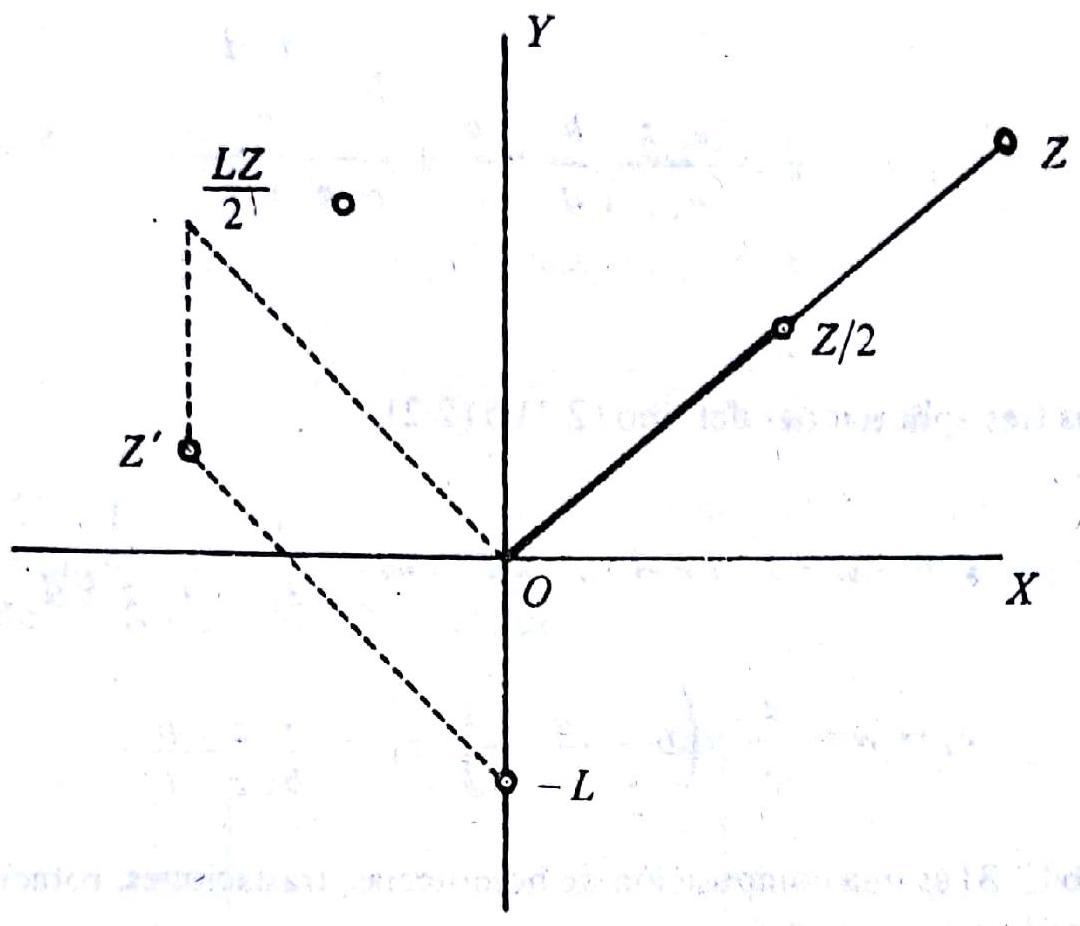
\includegraphics[width=\textwidth]{2025_09_05_adecef5eb2053bc129b5g-012}
\captionsetup{labelformat=empty}
\caption{Figura 1}
\end{center}
\end{figure}

\begin{enumerate}
  \setcounter{enumi}{2}
  \item Consideremos ahora la aplicación
\end{enumerate}


\begin{equation*}
z \mapsto \frac{1}{z} . \tag{2-2}
\end{equation*}


Como

$$
|z| \cdot\left|\frac{1}{z}\right|=1 \quad y \quad \arg z=-\arg \frac{1}{z}
$$

esta aplicación es geométricamente una inversión respecto de la circunferencia $|z|=1$, junto con una simetría respecto del eje OX .\\
4) Consideremos ahora la aplicación


\begin{equation*}
w=h(z)=\frac{a \cdot z+b}{c \cdot z+d} \tag{2-3}
\end{equation*}


en donde supondremos, para que $h$ no sea constante, que $a d-b c \neq 0$.\\
Descomponemos la aplicación (2-3)

$$
z \mapsto \frac{a \cdot z+b}{c \cdot z+d}=\frac{a}{c}+\frac{b-\frac{a \cdot d}{c}}{c \cdot z+d}
$$

en las tres aplicaciones del tipo (2-1) ó (2-2)

$$
\begin{aligned}
& z \mapsto z_{1}=c \cdot z+d, \quad z_{1} \mapsto z_{2}=\frac{1}{z_{1}}=\frac{1}{c \cdot z+d} \\
& z_{2} \mapsto w=\frac{a}{c}+\left(b-\frac{a \cdot d}{c}\right) z_{2}=\frac{a \cdot z+b}{c \cdot z+d}
\end{aligned}
$$

luego (2-3) es una composición de homotecias, traslaciones, rotaciones, una inversión y una simetría.

Podemos suponer $c \neq 0$, en caso contrario (2-3) se reduce a (2-1).\\
5) La aplicación $z \mapsto z^{2}$ actúa duplicando el argumento y elevando al cuadrado el módulo. Así por ejemplo, la imagen de la semicircunferencia:

$$
|z|=2 \quad, \quad 0 \leqslant \arg z \leqslant \pi
$$

es toda la circunferencia $|z|=4$.\\
Veamos ahora cuál es la condición de continuidad de una función compleja de variable compleja.

\begin{definition}
La aplicación $f$ de $\Omega \subset C$ en $C$ es continua en el punto $z_{0}$ si dado un $\varepsilon>0$ existe un $\delta>0$ tal que:
$$\left|z-z_{0}\right| \leqslant \delta \Rightarrow\left|f(z)-f\left(z_{0}\right)\right| \leqslant \varepsilon .$$
\end{definition}

Sea $f(z)=u(x, y)+i v(x, y)$ y $z_{0}=x_{0}+i y_{0}$.

Tomemos $x$ e $y$ tales que

$$
\left|x-x_{0}\right| \leqslant \frac{\delta}{2},\left|y-y_{0}\right| \leqslant \frac{\delta}{2},
$$

entonces

$$
\begin{aligned}
\left|z-z_{0}\right| \leqslant \delta \Rightarrow\left|u(x, y)+i v(x, y)-\left[u\left(x_{0}, y_{0}\right)+i v\left(x_{0}, y_{0}\right)\right]\right| \leqslant \varepsilon \Rightarrow & \\
& \Rightarrow\left\{\begin{array}{l}
\left|u(x, y)-u\left(x_{0}, y_{0}\right)\right| \leqslant \varepsilon \\
\left|v(x, y)-v\left(x_{0}, y_{0}\right)\right| \leqslant \varepsilon
\end{array}\right.
\end{aligned}
$$

es decir, las dos funciones $u$ y $v$ son continuas en el punto ( $x_0, y_0$ ).\\
Recíprocamente si $u(x, y)$ y $v(x, y)$ son ambas continuas en ( $x_0, y_0$ ), entonces dado $\varepsilon>0$ existe un $\eta>0$ tal que

$$
\left.\left|x-x_{0}\right| \leqslant \eta\right\} \Rightarrow\left\{\begin{array}{l}
\left|u(x, y)-u\left(x_{0}, y_{0}\right)\right| \leqslant \frac{\varepsilon}{2} \\
\left|v(x, y)-v\left(x_{0}, y_{0}\right)\right| \leqslant \frac{\varepsilon}{2}
\end{array}\right\} \Rightarrow\left|f(z)-f\left(z_{0}\right)\right| \leqslant \varepsilon,
$$

luego

$$
\left|z-z_{0}\right| \leqslant \eta \Rightarrow\left\{\begin{array}{c}
\left|x-x_{0}\right| \leqslant \eta \\
\left|y-y_{0}\right| \leqslant \eta
\end{array}\right\} \Rightarrow\left|f(z)-f\left(z_{0}\right)\right| \leqslant \varepsilon .
$$

Es decir: una función compleja de variable compleja es continua si, y sólo si, son continuas sus partes real e imaginaria.

Consideraciones análogas pueden hacerse para el límite en un punto, que se reduce a la existencia de límite de las partes real e imaginaria.

Se ve por consiguiente que los límites y la continuidad de las funciones complejas se reducen a los límites y continuidad de pares de funciones reales de dos variables reales. Podría creerse a primera vista que la derivabilidad de la función $f(z)$ es reducible a la de sus partes real e imaginaria, pero se verá ahora que ello no es así. La derivación en el dominio complejo presenta características muy diferentes a las del caso real y esas diferencias son las que dan interés a la teoría.


\section{Funciones holomorfas}
Sea $f$ una aplicación de un conjunto $\Omega$ abierto y conexo de $C$, en $C$ y $z$ un punto de $\Omega$.

\begin{definition}
La derivada de $f$ en el punto $z$ es el número complejo $f'(z)$ definido por
\begin{equation*}
\lim _{\Delta z \rightarrow 0} \frac{f(z+\Delta z)-f(z)}{\Delta z}=f^{\prime}(z) \tag{3-1}
\end{equation*}
cuando este límite existe.
\end{definition}

Veamos sus condiciones de existencia. Pongamos

$$
\begin{aligned}
& f^{\prime}(z)=a+i b \\
& f(z+\Delta z)-f(z)=\Delta f=\Delta u+i \Delta v \\
& \Delta z=\Delta x+i \Delta y=\rho(\cos \varphi+i \operatorname{sen} \varphi) ; \\
& \rho^{2}=\Delta x^{2}+\Delta y^{2} .
\end{aligned}
$$

Así la condición (3-1) es equivalente a

\[
\left.\begin{array}{l}
\Delta f=\Delta z \cdot f^{\prime}(z)+\Delta z \mu(\Delta z)  \tag{3-2}\\
\lim _{\Delta z \rightarrow 0} \mu(\Delta z)=0
\end{array}\right\}
\]

Poniendo $\mu(\Delta z)$ en la forma polar $\mu(\Delta z)=r(\cos \lambda+i \operatorname{sen} \lambda)$; en donde $r$ y $\lambda$ son funciones de $\Delta z$, (o de $\Delta x$ y $\Delta y$, o de $\rho$ y $\varphi$) se cumple:


\begin{equation*}
\lim _{\rho \rightarrow 0} r=0 . \tag{3-3}
\end{equation*}


La condición (3-2) puede ponerse en la forma

$$
\Delta u+\Delta v i=(a+i b)(\Delta x+i \Delta y)+\rho r[\cos (\varphi+\lambda)+i \operatorname{sen}(\varphi+\lambda)] .
$$

Igualando partes real e imaginaria se tiene

\[
\left.\begin{array}{l}
\Delta u=a \Delta x-b \Delta y+\rho r \cos (\varphi+\lambda)  \tag{3-4}\\
\Delta v=b \Delta x+a \Delta y+\rho r \operatorname{sen}(\varphi+\lambda) \\
\lim _{\rho \rightarrow 0} r=0
\end{array}\right\}
\]

Las condiciones (3-1) y (3-4) son entonces equivalentes.
Pero (3-4) significa que las dos funciones $u$ y $v$ son diferenciables en el punto $(x, y)$ y además que

$$
u_{x}^{\prime}=v_{y}^{\prime}=a \quad ; \quad-u_{y}^{\prime}=v_{x}^{\prime}=b
$$

Luego tenemos:

\begin{theorem}[Cauchy-Riemann]
Para que la función $f=u+iv$ sea derivable en un punto es necesario y suficiente que las dos funciones $u$ y $v$ sean diferenciables en ese punto y además que en dicho punto se cumplan las denominadas condiciones de Cauchy-Riemann:
$$u_{x}^{\prime}=v_{y}^{\prime} \quad ; \quad u_{y}^{\prime}=-v_{x}^{\prime} .$$
Entonces la derivada de $f$ en el punto $z$ es
\begin{equation*}
f^{\prime}(z)=u_{x}^{\prime}+i v_{x}^{\prime}=u_{x}^{\prime}-i u_{y}^{\prime}=v_{y}^{\prime}+i v_{x}^{\prime}=v_{y}^{\prime}-i u_{y}^{\prime} \tag{3-5}
\end{equation*}
\end{theorem}

Vemos, pues, que la derivabilidad de $f$ no sólo implica la derivabilidad de $u$ y de $v$, sino además una estrecha relación entre ellas dada por las ecuaciones de Cauchy-Riemann.

\begin{definition}
Se dice que $f$ es monógena en un punto $z_{0}$ si tiene derivada en dicho punto y se dice que es holomorfa en el punto si tiene derivada en todos los puntos de un entorno de $z_{0}$.
\end{definition}

Hay autores que no establecen la diferencia entre funciones monógenas y holomorfas.

Se supone siempre que $f$ está definida en un conjunto $\Omega$ abierto. Cuando sea holomorfa en todos los puntos de $\Omega$ diremos que es holomorfa en $\Omega$.

\begin{example}
Sea la función $f$ definida en todo el plano como
$$x+i y \stackrel{f}{\longmapsto} x^{2}+i y^{2} .$$
Se tiene:
$$u_{x}^{\prime}=2 x \quad ; \quad u_{y}^{\prime}=0 \quad ; \quad v_{x}^{\prime}=0 \quad ; \quad v_{y}^{\prime}=2 y .$$
Las funciones $u$ y $v$ son diferenciables en todo el plano, pero sólo cumplen las condiciones de Cauchy-Riemann sobre la recta $y=x$. Sobre ella $f$ es monógena, pero no holomorfa.
\end{example}

Como la definición (3-1) de derivada es la misma que la dada para las funciones reales de variable real, se puede deducir que:
$1^{\circ}$) Toda función monógena es continua.
$2^{\circ}$) Las reglas formales de derivación demostradas en el caso real para suma, producto, cociente, función de función, función inversa, etc., se extienden en forma automática al campo complejo.

En particular, los polinomios son funciones holomorfas en todo el plano; las funciones racionales lo son en el conjunto complementario de los ceros del denominador. La suma o producto de funciones holomorfas es holomorfa, así como también el cociente en los puntos en que no se anule el denominador.

\begin{theorem}
Una función $f$ definida en $\Omega$ abierto y conexo es constante si, y sólo si, $f'(z)=0$ en todos los puntos de $\Omega$.
\end{theorem}

\begin{proof}
Basta ver que:
$$f^{\prime}=0 \Longleftrightarrow\left\{\begin{array}{l}
u_{x}^{\prime}=u_{y}^{\prime}=0 \\
v_{x}^{\prime}=v_{y}^{\prime}=0
\end{array}\right\} \Longleftrightarrow\left\{\begin{array}{l}
u=\text { cte } \\
v=\text { cte }
\end{array}\right\} \Longleftrightarrow f=\text { cte } .$$
\end{proof}

Consideremos ahora una función $f$ holomorfa en $\Omega$ (abierto y conexo) y hagamos la hipótesis suplementaria de la existencia y continuidad de las derivadas segundas de $u$ y $v$. Más adelante veremos que esta condición es superflua.

Calculando los laplacianos de $u$ y $v$, y aplicando las condiciones de Cauchy-Riemann

$$
\begin{aligned}
& \Delta u=u_{x}^{\prime \prime}+u_{y}^{\prime \prime}=\frac{\partial}{\partial x} v_{y}^{\prime}-\frac{\partial}{\partial y} v_{x}^{\prime}=v_{x y}^{\prime \prime}-v_{y x}^{\prime \prime}=0 ; \\
& \Delta v=v_{x x}^{\prime \prime}+v_{y y}^{\prime \prime}=\frac{\delta}{\partial x} u_{y}^{\prime}+\frac{\partial}{\partial y} u_{x}^{\prime}=u_{x y}^{\prime \prime}-u_{y x}^{\prime \prime}=0 .
\end{aligned}
$$

Es decir, las partes real e imaginaria de una función holomorfa son funciones armónicas.

Sea ahora una función $u(x, y)$ armónica en $\Omega$. Vamos a ver que existe una función $f$ holomorfa en $\Omega$ "única salvo la adición de una constante imaginaria pura" cuya parte real es $u(x, y)$.

En efecto, basta determinar la parte imaginaria $\nu(x, y)$, la cual debe cumplir las condiciones

$$
v_{x}^{\prime}=-u_{y}^{\prime} \quad, \quad v_{y}^{\prime}=u_{x}^{\prime}
$$

Como de la teoría de las diferenciales exactas sabemos que debe verificarse

$$
-u_{y^{\prime}}^{\prime \prime}=\frac{\partial v_{x}^{\prime}}{\partial y}=\frac{\partial v_{y}^{\prime}}{\partial x}=u_{x x}^{\prime \prime},
$$

pero esta condición se cumple por la hipótesis de la armonicidad de $u$; la función $v$ resulta así definida salvo una constante y por lo tanto $f=u+i v$ queda definida a menos de una constante imaginaria pura.

\begin{example}
Sea $u(x, y)=x^{3}-3 x y^{2}$,
$$\Delta u=u_{x^{2}}^{\prime \prime}+u_{y^{2}}^{\prime \prime}=6 x-6 x=0$$
luego $u$ es armónica. La función $v$ a determinar debe cumplir las condiciones
$$v_{x}^{\prime}=6 x y \quad ; \quad v_{y}^{\prime}=3 x^{2}-3 y^{2} .$$
Integrando $v_{x}$ respecto de la variable $x$ se tiene
$$v(x, y)=3 x^{2} y+\alpha(y) .$$
Derivando respecto de $y$,
$$v_{y}^{\prime}=3 x^{2}-3 y^{2}=3 x^{2}+\alpha^{\prime}(y) \Rightarrow \alpha^{\prime}(y)=-3 y^{2} .$$
Integrando la función $\alpha^{\prime}(y)$ resulta
$$v(x, y)=3 x^{2} y-y^{3}+C$$
De aquí,
$$f(z)=x^{3}-3 x y^{2}+3 x^{2} y i-y^{3} i+i C=(x+i y)^{3}+i C=z^{3}+i C$$
\end{example}

Naturalmente que un procedimiento enteramente análogo puede usarse para determinar una función holomorfa cuya parte imaginaria sea una función armónica dada.

Veamos ahora una propiedad geométrica importante de la función holomorfa.

Sea $w=f(z)$ una función holomorfa en un dominio $\Omega$. Sea $z_{0}$ un punto de $\Omega w_{0}=f\left(z_{0}\right)$ y supongamos $f^{\prime}\left(z_{0}\right) \neq 0$ (condición esencial). Sea $\varphi_{0}=\arg f^{\prime}\left(z_{0}\right)$. Por la defínición de derivada,

$$
\lim _{z \rightarrow z_{0}} \frac{f(z)-f\left(z_{0}\right)}{z-z_{0}}=f^{\prime}\left(z_{0}\right)
$$

luego


\begin{equation*}
\lim _{z \rightarrow z_{0}}\left\{\arg \left[f(z)-f\left(z_{0}\right)\right]-\arg \left[z-z_{0}\right]\right\}=\varphi_{0} . \tag{3-6}
\end{equation*}


Sea ahora $\gamma$ una curva de origen $z_{0}$ situada en el plano de las $z$. Sea $\Gamma=f(\gamma)$ su imagen en el plano $w$. Suponemos que $\gamma$ y $\Gamma$ admiten tangentes $t$ y $T$ en los puntos $z_{0}$ y $w_{0}=f\left(z_{0}\right)$ respectivamente.

\begin{figure}[h]
\begin{center}
  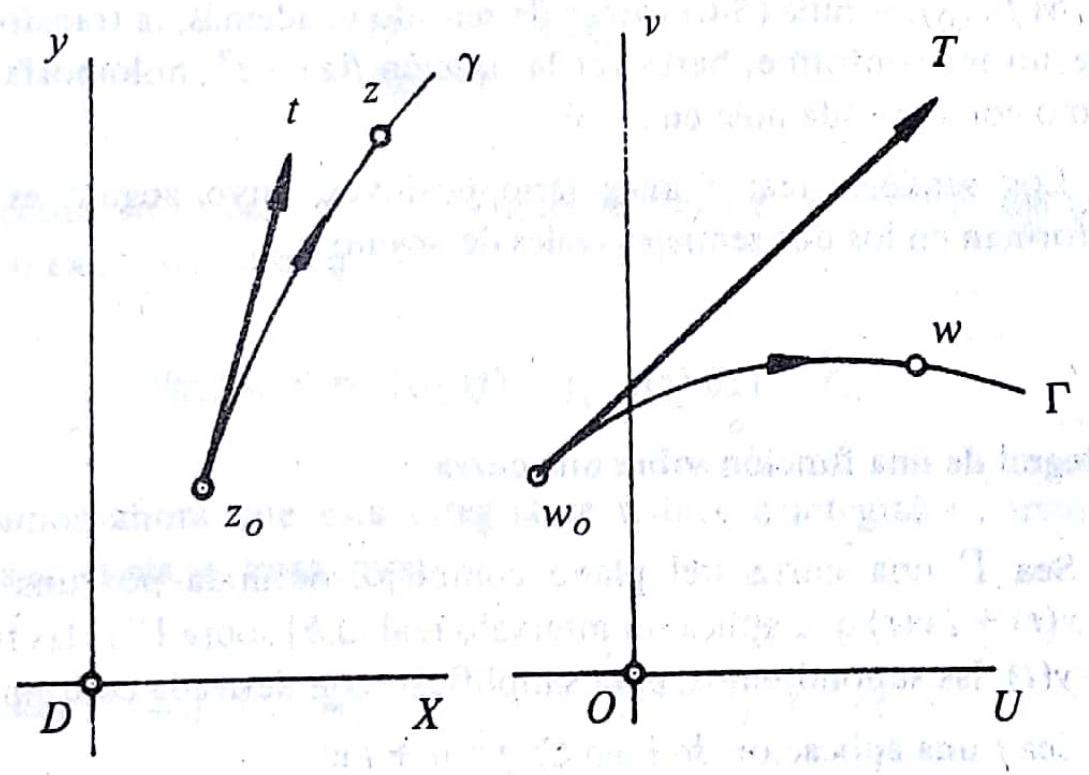
\includegraphics[width=\textwidth]{2025_09_05_adecef5eb2053bc129b5g-020}
\captionsetup{labelformat=empty}
\caption{Figura 2}
\end{center}
\end{figure}

Si hacemos tender $z$ hacia $z_{0}$ a lo largo de $\gamma$, la cuerda $z-z_{0}$ tiende hacia la tangente $t$; es decir. el argumento de $z-z_{n}$ tiende hacia el ángulo formado por $t$ con el semieje positivo de las $x$. Además $f^{\prime}(z)$ tiende hacia wo y el argumento de $f(z)-f\left(z_{0}\right)$ tiende hacia el ángulo formado por $T$ con el semieje positivo de las $u$. Luego teniendo en cuenta (3-6) se tiene

$$
\operatorname{áng}\left(t, O_{x}\right)=\operatorname{ang}\left(T, O_{u}\right)-\varphi_{0}
$$


Consideremos ahora otra curva $\gamma^{\prime}$ de tangente $t^{\prime}$ y sean $\Gamma^{\prime}=f\left(\gamma^{\prime}\right)$ y $T^{\prime}$ la tangente a $\Gamma^{\prime}$ ', como anteriormente. Se tiene

$$
\text { áng }\left(t^{\prime}, 0_{x}\right)=\text { áng }\left(T^{\prime}, 0_{u}\right)-\varphi_{0} \text {. }
$$

Restando las dos igualdades se tiene


\begin{equation*}
\operatorname{áng}\left(t, t^{\prime}\right)=\operatorname{áng}\left(T, T^{\prime}\right) \text {. } \tag{3-7}
\end{equation*}


Es decir, el ángulo de dos curvas es igual al ángulo de sus transformados por f . La transformación de $f$ - que conserva los ángulos (en valor absoluto y sentido) se llama conforme.

Observemos que de (3-6) se deduce que si una curva tiene tangente en un punto, su transformada también la tiene.

Si $f^{\prime}\left(z_{0}\right)$ es nula (3-6) carece de sentido y, además, la transformación puede no ser conforme; basta ver la función $f(z)=z^{2}$, holomorfa en todo el plano con derivada nula en $z=0$.

Los semiejes real e imaginario positivos, cuyo ángulo es $\pi / 2$, se transforman en los dos semiejes reales de ángulo $\pi$.

\section{Integral de una función sobre una curva}
Sea $\Gamma$ una curva del plano complejo, definida por una función $z(t)=x(t)+i y(t)$ que aplica un intervalo real $[a, b]$ sobre $\Gamma$. A las funciones $x(t)$ e $y(t)$ las supondremos, para simplificar, con derivada continua:

Sea $f$ una aplicación de $\Gamma$ en $C ; f=u+i v$\\
Sea $\pi$ una partición de $[a, b]$ definida por los números $t$, $a=t_{0}<t_{1}<\ldots<t_{n}=b$ y sean

$$
\xi_{j} \in\left[t_{j-1}, t_{j}\right], z_{j}=z\left(t_{j}\right), \quad j=1,2, \ldots, n .
$$

La suma de Riemann $\sigma_{\pi}(\mathrm{f})$ de f respecto de $\pi$ es por definición el número complejo

$$
\sigma_{\pi}(f)=\sum_{1}^{\mathrm{n}} f\left(\xi_{j}\right) \Delta z_{j}, \text { con } \Delta z_{j}=z_{j}-z_{j-1}, j=1,2, \ldots, n
$$

A partir de aquí la definición de la integral sigue el mismo camino que en el caso real.

Se llama módulo de $\pi$ al número real positivo

$$
\sup \left|t_{j}-t_{j-1}\right|=\|\pi\|
$$

La integral de f sobre $\Gamma$,

$$
I=\int_{\Gamma} f(z) d z
$$

es por definición el límite

$$
\lim _{||\pi| \mapsto 0} \sigma_{\pi}(f)
$$

donde -como en el caso real- el límite se toma en el sentido siguiente: dado $\varepsilon>0$ existe $\delta>0$ tal que

$$
\|\pi\|<\varepsilon \Rightarrow\left|\sigma_{\pi}(f)-\int_{\Gamma} f(z) d z\right|<\varepsilon
$$

Veamos ahora que esta integral se reduce a integrales curvilíneas ordinarias en el plano. Pongamos

$$
\begin{aligned}
\Delta z_{j} & =\Delta x_{j}+i \Delta y_{j} \quad, \quad \xi_{j}=\alpha_{j}+i \beta_{j} \\
\sigma_{\pi}(f) & =\sum_{j=1}^{m}\left[u\left(\alpha_{j}, \beta_{j}\right)+i v\left(\alpha_{j}, \beta_{j}\right)\right] \cdot\left[\Delta x_{j}+i \Delta y_{j}\right]= \\
& =\sum_{j=1}^{m}\left[u\left(\alpha_{j}, \beta_{j}\right) \Delta x_{j}-v\left(\alpha_{j} ; \beta_{j}\right) \Delta y_{j}\right]+ \\
& +i \sum_{j=1}^{m}\left[v\left(\alpha_{j}, \beta_{j}\right) \Delta x_{j}+u\left(\alpha_{j}, \beta_{j}\right) \Delta y_{j}\right]
\end{aligned}
$$


Las dos sumas del último miembro son las sumas de Riemann que definen las integrales curvilíneas

$$
\int_{\Gamma}(u d x-\nu d y) \quad ; \quad \int_{\Gamma}(\nu d x+u d y)
$$

luego podemos escribir


\begin{equation*}
\int_{\Gamma} f(z) d z=\int_{\Gamma}(u d x-\nu d y)+i \int_{\Gamma}(v d x+u d y) \tag{41}
\end{equation*}


y la igualdad implica también que la integral de $f$ a lo largo de $\Gamma$ existe si, y sólo si, existen las dos integrales curvilíneas. De acuerdo con la teoría, la integral existirá cuando $f$ sea continua y $\Gamma$ rectificable.

Nosotros supondremos además, como dijimos al principio, que la función $z(t)$ tiene derivada continua. Vamos a ver cómo se puede calcular la integral en este caso. Se tiene

$$
\begin{aligned}
\int_{\Gamma} f(z) d z & =\int_{\Gamma}[(u d x-v d y)+i(v d x+u d y)] \\
& =\int_{a}^{b}\left\{\left(u x^{\prime}-v y^{\prime}\right)+i\left(v x^{\prime}+u y^{\prime}\right)\right\} d t \\
& =\int_{a}^{b}\left\{(u+i v) \cdot\left(x^{\prime}+i y\right)\right\} d t=\int_{a}^{b} f[z(t)] \cdot z^{\prime}(t) d t
\end{aligned}
$$

es decir, se obtiene una regla de cálculo completamente análoga a la de las integrales curvilíneas ordinarias.

Vamos a aplicar este método al cálculo de la integral

$$
I_{n}=\int_{C_{r}}\left(z-z_{0}\right)^{n} d z
$$

donde $n$ es un número entero y $C_{r}$ es la circunferencia $\left[z-z_{0}\right]=r$ de ecuación paramétrica

$$
z=z_{0}+r(\cos t+i \operatorname{sen} t)
$$

$\operatorname{con} t \in[0,2 \pi)$, recorrida en sentido positivo:

$$
\begin{aligned}
& \left(z-z_{0}\right)^{n}=r^{n}(\cos n t+i \operatorname{sen} n t) \\
& d z=r(-\operatorname{sen} t+i \cos t)=i r(\cos t+i \operatorname{sen} t)
\end{aligned}
$$

luego:

$$
I_{n}=\int_{0}^{2 \pi} i r^{n+1}[\cos (n+1) t+i \operatorname{sen}(n+1) t \mid d t
$$

así para $n+1 \neq 0$, es decir, $n \neq-1$, se tiene $I_{n}=0$; para $n=-1$.

$$
I_{-1}=\int_{0}^{2 \pi} i d t=2 \pi i
$$

es decir,

\[
\int_{\left.C_{i r}\right)}\left(z-z_{0}\right)^{n} d z=\left\{\begin{array}{l}
\cup \text { para } n \in L, n \neq-1  \tag{4-2}\\
2 \pi i \text { para } n=-1
\end{array}\right.
\]

Las integrales de funciones de variable compleja tienen las misma propiedades de linealidad y aditividad que las integrales curvilíneas, en virtud de la fórmula (4-1). Demostraremos una importante fórmula de mayoración. Supongamos que para todo $z \in \Gamma$ sea $|f(z)| \leqslant M$, entonces para una suma de Riemann cualquiera se tiene

$$
\left|\sigma_{\pi}(J)\right| \leqslant \sum_{1}^{n}\left|f\left(\xi_{j}\right)\right| \cdot\left|\Delta z_{j}\right| \leqslant M \sum_{1}^{n}\left|\Delta z_{j}\right|
$$

pero $\Sigma\left|\Delta_{z}\right|$ es la longitud de la poligonal de vértices $z_{0}, z_{1}, \ldots, z_{m}$, que es menor que la longitud de la curva $\Gamma$. Es decir, $\left|\sigma_{\pi}(f)\right| \leqslant M$. long $(\Gamma)$ para toda partición $\pi$.

Luego la desigualdad vale para el límite y se tiene la importante fórmula de mayoración.


\begin{equation*}
\left|y^{\prime}(z)\right| \leqslant M \quad, \quad \forall z \in \Gamma \Rightarrow\left|\int_{\Gamma} f(z) d z\right| \leqslant M, L, \tag{$4\cdot3$}
\end{equation*}


donde $L$ es la longitud de la curva $\Gamma$.

\section{Teorema y fórmula de Cauchy}

\begin{theorem}[Teorema de Cauchy]
Consideremos ahora un conjunto $\Omega$ abierto y simplemente conexo. Sea $\Gamma$ una curva cerrada rectificable y simple (es decir, sin puntos múltiples) contenida en $\Omega$ y sea $f$ una función holomorfa cuya derivada en $\Omega$ es una función continua. Entonces la integral de $f$ a lo largo de $\Gamma$ es cero.
\end{theorem}

\begin{proof}
La fórmula (4-1) dice que:
$$\int_{\Gamma} f(z) d z=\int_{\Gamma}(u d x-v d y)+i \int_{\Gamma}(v d x+u d y)$$
pero las condiciones de Cauchy-Riemann
$$u_{y}^{\prime}=-v_{x}^{\prime} \quad y \quad v_{y}^{\prime}=u_{x}^{\prime},$$
implican que las diferenciales $u d x-v d y$ y $v d x+u d y$ son exactas en el conjunto simplemente conexo $\Omega$. Luego sus integrales a lo largo de una curva cerrada son nulas, y esto concluye la prueba.
\end{proof}

La demostración que hemos dado del teorema de Cauchy es muy fácil, pero esa facilidad se ha conseguido imponiendo demasiadas hipótesis: en particular, la continuidad de la derivada es superflua. Aun cuando la forma que hemos dado es suficiente para nuestras necesidades enunciaremos el teorema en una forma más general.

\begin{theorem}[Teorema de Cauchy-Goursat]
Sea $f$ holomorfa en un abierto $\Omega$ simplemente conexo; sea $\Gamma$ la frontera de $\Omega$ que supondremos es una curva cerrada simple rectificable y suponemos además que $f$ es continua en $\Omega \cup \Gamma$. Entonces
$$\int_{\Gamma} f(z) d z=0$$
\end{theorem}

El ieorema puede extenderse a casos en que el dominio no es simplemente conexo. Tomemos el caso más simple: un conjunto simplemente conexo del que se retira un disco contenido en el conjunto.

\begin{figure}[h]
\begin{center}
  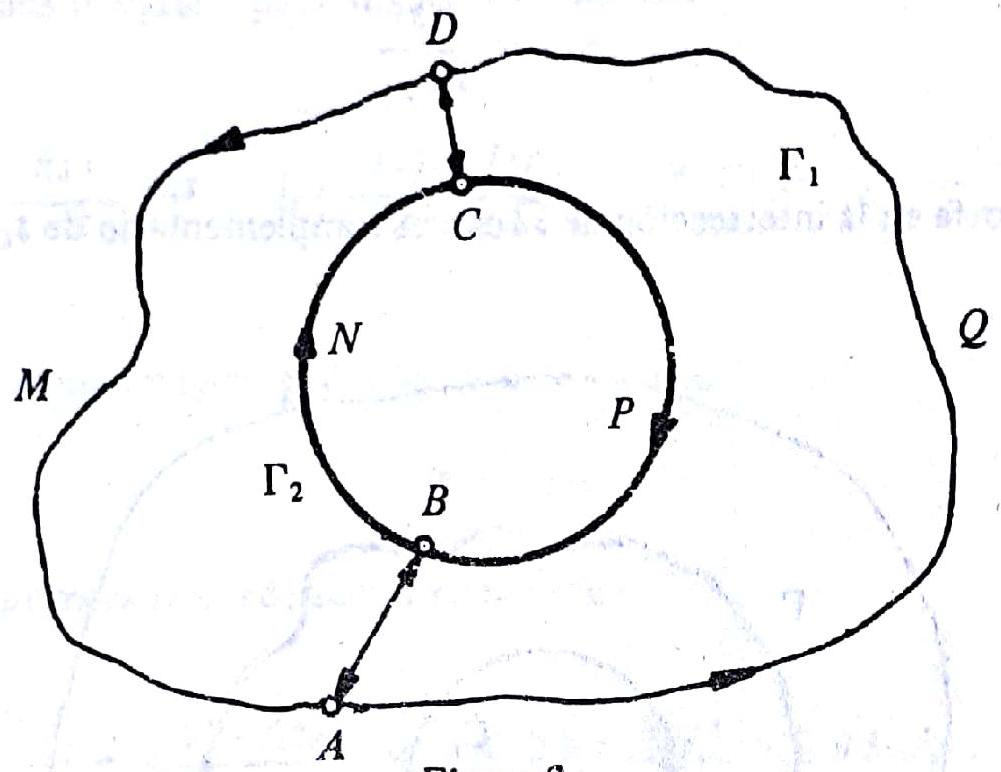
\includegraphics[width=\textwidth]{2025_09_05_adecef5eb2053bc129b5g-026}
\captionsetup{labelformat=empty}
\caption{Figura 3}
\end{center}
\end{figure}

El teorema es aplicable al contomo ABNCDMA y al AQDCPBA.\\
Sumando las dos integrales se tiene:\\
$\int_{\overline{\mathrm{AB}}} f+\int_{\widehat{\mathrm{BNC}}} f+\int_{\overline{\mathrm{CD}}} f+\int_{\widehat{\mathrm{DMA}}} f+\int_{\widehat{\mathrm{AQD}}} f+\int_{\overline{\mathrm{DC}}} f+\int_{\widehat{\mathrm{CPB}}} f+\int_{\overline{\mathrm{BA}}} f=0$\\
Sea $\Gamma_{1}$ el contomo exterior AQDMA y $\Gamma_{2}$ el contorno interior BNCPB ; las integrales sobre $\overline{\mathrm{AB}}$ y $\overline{\mathrm{BA}}$ son iguales y de signo contrario; lo mismo sucede con las integrales sobre $\overline{C D}$ y $\overline{D C}$; luego llamando $\Gamma$ a la reunión de $\Gamma_{1}$ y $\Gamma_{2}$ se tiene:

$$
\int_{\Gamma} f(z) d z=0
$$

Naturalmente, el sentido de recorrido debe ser tal que el dominio de holomorfismo quede de un mismo lado a medida que se describa la curva $\Gamma$.

Es claro que este resultado puede extenderse si en vez de extraer un disco se quita un número finito de discos.


Consideremos ahora una función holomorfa en un abierto simplemente conexo $\Omega ; \Gamma$ una curva cerrada simple rectificable contenida en $\Omega_{y} z_{0}$ un punto interior del dominio $\Omega$ ' limitado por $\Gamma$. Tracemos una circun. ferencia $C_{\boldsymbol{r}}$ de radio $r$ contenida en $\Omega^{\prime}$.

La función

$$
\varphi(z)=\frac{f(z)}{z-z_{0}}
$$

es holomorfa en la intersección de $\Omega$ con el complementario de $z_{0}$.

\begin{figure}[h]
\begin{center}
  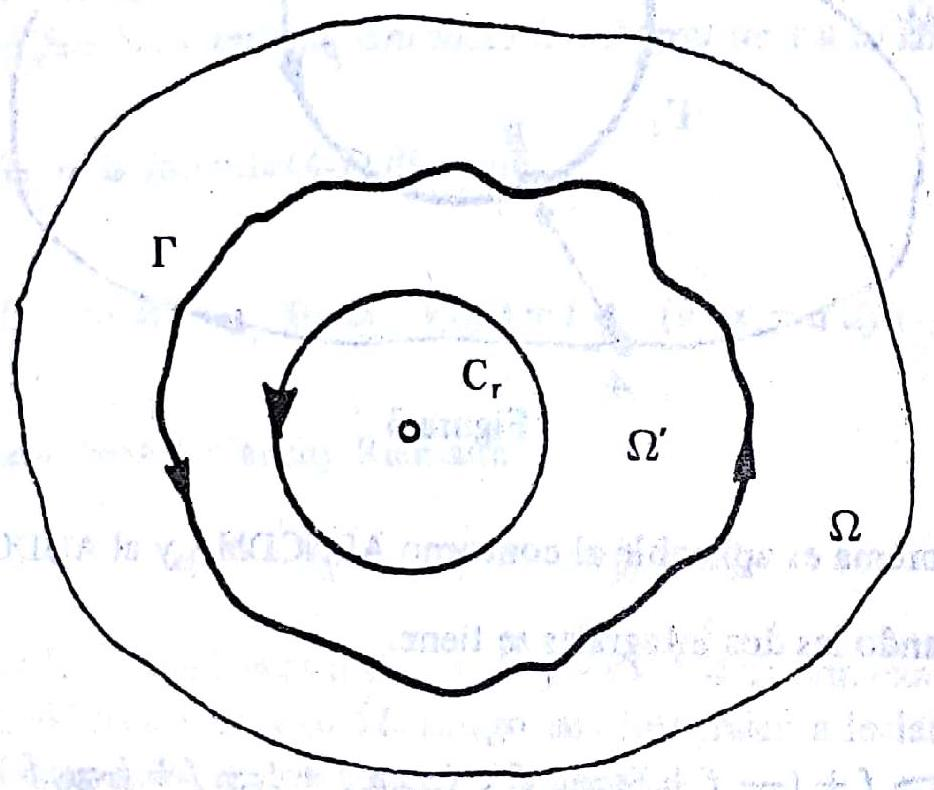
\includegraphics[width=\textwidth]{2025_09_05_adecef5eb2053bc129b5g-027}
\captionsetup{labelformat=empty}
\caption{Figura 4}
\end{center}
\end{figure}

Podemos aplicar entonces el teorema de Cauchy en la forma que acabamos de enunciar. Tenemos:

$$
\int_{\Gamma^{+}} \frac{f(z)}{z-z_{0}} d z+\int_{C_{r}} \frac{f(z)}{z-z_{0}} d z=0
$$

indicando con $\Gamma^{+}$y con $C^{\prime} \dot{r}$ las curvas $\Gamma$ y $C^{\prime}$ recorridas en el sentido ${ }^{\circ}$ del dibujo la primera y en el sentido contrario la segunda.

\section*{Sumando y restando}
$$
\frac{f\left(z_{0}\right)}{z-z_{0}}
$$

en la segunda integral y pasando al otro miembro


\begin{equation*}
\int_{\Gamma^{+}} \frac{f(z)}{z-z_{0}} d z=\int_{C_{r}^{+}} \frac{f(z)-f\left(z_{0}\right)}{z-z_{0}} d z+f\left(z_{0}\right) \int_{C_{r}^{+}} \frac{d z}{z-z_{0}} . \tag{4-4}
\end{equation*}


La última integral, por la fúrmula (4-2), vale

$$
2 \pi i . j(20) .
$$

La primera se puede acotar en la forma

$$
\left|\int_{C_{r}^{+}} \frac{f(z)-f\left(z_{0}\right)}{z-z_{0}} d z\right| \leqslant 2 \pi r \frac{M(r)}{r}=2 \pi M(r)
$$

en donde $M(r)$ es el máximo de $\left|f(z) \cdot f\left(z_{0}\right)\right|$ en $C_{r}$ : por la continuidad de $f$ resulta

$$
\lim _{r \rightarrow 0} M(r)=0 .
$$

Tomando límites en (4-4) para $r \rightarrow 0$ se tiene la llamada fórmula de Cauchy.


\begin{equation*}
f\left(z_{0}\right)=\frac{1}{2 \pi i} \int_{\Gamma^{+}} \frac{f(z)}{z-z_{0}} d z \tag{45}
\end{equation*}


que nos da el valor de f en un punto interior en función únicamente de los valores en la frontera.

Vemos aquí una propiedad inherente al campo complejo y $\sin$ equivalente en el campo real: con la sola hipótesis de derivabilidad. el\\
conocimiento de la función en un subconjunto (la frontera) basta para determinar completamente la función en todo su dominio.

\section{Funciones primitivas}
Como en el caso real, se dice que una función $F$ es la primitiva de otra $f$ (ambas con el mismo dominio de definición) cuando $f$ es la derivada de $F$. Si $\Phi$ es otra primitiva'de $f$, la derivada de $F-\Phi$ es cero, lo que implica que $F$ - $\Phi$ es constante ( $\Phi 2$, teorema 2 ). Recíprocamente si a $F$ se le suma una constante, se obtiene una nueva primitiva de $f$.

Supongamos ahora que tenemos una función $f$ definida y continua en $\Omega$ abierto y conexo y otra función $F$ primitiva de $f$ en $\Omega$, entonces cualquiera sea la curva $\gamma$ rectificable y contenida en $\Omega$, de origen $\mathrm{z}_{1}$ y extremo $z_{2}$ se tiene la fórmula de Barrow.

$$
\int_{\gamma} f(z) d z=F\left(z_{2}\right)-F\left(z_{1}\right) .
$$

En efecto: tenemos

$$
f=u+i v \quad ; \quad F=A+i B
$$

y las ecuaciones de Cauchy-Riemann

$$
A_{x}^{\prime}=B_{y}^{\prime}=u \quad \therefore \quad-A_{y}^{\prime}=B_{x}^{\prime}=v
$$

y, por lo tanto,

$$
\begin{aligned}
\int_{\gamma} f(z) d z & =\int_{\gamma}(u d x-v d y)+i \int_{\gamma}(v d x+u d y)= \\
& =\int_{\gamma}\left(A_{x}^{\prime} d x+A_{y}^{\prime} d y\right)+i \int_{\gamma}\left(B_{x}^{\prime} d x+B_{y}^{\prime} d y\right)= \\
& =\int_{\gamma} d A+i \int_{\gamma} d B=A\left(z_{2}\right)-A\left(z_{1}\right)+i\left[B\left(z_{2}\right)-B\left(z_{1}\right)\right]= \\
& =F\left(z_{2}\right)-F\left(z_{1}\right)
\end{aligned}
$$

La fórmula de Barrow tiene un tipo de propiedad recíproca que es la siguiente:

Si $f$, continua en $\Omega$, es tal que para todo par de puntos $z_{1}$ y $z_{2}$ la integral

$$
\int_{P} f(z) d z
$$

es la misma para toda poligonal $\rho$ de origen $z_{1}$ y extremo $z_{2}$ contenida en $\Omega$, y en particular si $f$ es holomorfa en $\Omega$, entonces $f$ es la derivada de la función

$$
F(z)=\int_{a}^{z} f(\xi) d \xi
$$

en donde $a$ es un punto cualquiera fijo de $\Omega$ y la integral se toma sobre cualquier poligonal contenida en $\Omega$ de origen $a$ y extremo un punto $z$ variable de $\Omega$.

En efecto: sea $z_{0} \in \Omega$ y $z$ un punto de un disco de centro $z_{0}$ contenido en $\Omega$, sea $k=z-z_{0}$,

$$
\frac{F(z)-F\left(z_{0}\right)}{z-z_{0}}=\frac{F\left(z_{0}+k\right)-F\left(z_{0}\right)}{k}=\frac{1}{k} \int_{z_{0}}^{z_{0}+k} f(\xi) d \xi
$$

Como una primitiva de la constante 1 es $z$, se tiene

$$
\int_{z_{0}}^{z_{o^{+}}} d \xi=k \quad ; \quad f\left(z_{0}\right)=\frac{1}{k} \int_{z_{0}}^{z_{o^{+}}} f\left(z_{0}\right) d \xi
$$

las integrales se toman sobre el segmento de extremos $z_{0}$ y $z_{0}+k$.\\
Se tiene entonces, llamando $M(k)$ al supremo de $\left|f(\xi)-f\left(z_{0}\right)\right|$ en el segmento $\left[z_{0}, z_{0}+k\right]$, que $\lim _{k \rightarrow 0} M(k)=0$ y por lo tanto,

$$
\begin{aligned}
& \left|\frac{F(z)-F\left(z_{0}\right)}{z-z_{0}}-f\left(z_{0}\right)\right|=\frac{1}{|k|}\left|\int_{2_{0}}^{z_{0}+k}\left[f(\xi)-f\left(z_{0}\right)\right]\right| d \xi \leqslant \\
& \leqslant \frac{1}{|k|}|k| M(k) \xrightarrow[k \rightarrow 0]{ } 0
\end{aligned}
$$


Luego por definición de derivada

$$
F^{\prime}\left(z_{0}\right)=f\left(z_{0}\right) .
$$

\section{Sucesiones y series numéricas en el campo complejo}
Una sucesión $\left\{z_{n}\right\}$ de números complejos se define como una aplicación $n \rightarrow z_{n}$ del conjunto de los números naturales en el de los complejos.

\section*{DEFINICION 1}
Se dice que $\alpha \in \mathrm{C}$ es el límite de la sucesión $z_{n}$,

$$
\alpha=\lim _{n \rightarrow \infty} z_{n},
$$

si para todo $\varepsilon>0$, existe $\mathrm{n}_{0}$ natural tal que


\begin{gather*}
n \geqslant n_{0} \Rightarrow z_{n}-\alpha \mid \leqslant \varepsilon .  \tag{7-1}\\
\text { Pongamos } z_{n}=x_{n}+i y_{n}, \alpha=a+i b . \text { Se tiene } \\
0 \leqslant \sup \left\{\left|x_{n}-a\right|, \mid y_{n}-b i\right\} \leqslant\left|z_{n}-\alpha\right| \leqslant\left|x_{n}-a\right|+\left|y_{n}-b\right|
\end{gather*}


y estas desigualdades implican, naturalmente,


\begin{equation*}
\lim _{n \rightarrow \infty} z_{n}=\alpha \Leftrightarrow \lim _{n \rightarrow \infty} x_{n}=a \quad \text { y } \quad \lim _{n \rightarrow \infty} y_{n}=b \tag{7-2}
\end{equation*}


es decir, la convergencia de la sucesión se reduce a la convergencia de las partes real e imaginaria.

Como el criterio de Cauchy es válido en el campo real, de lo que acabamos de decir se deduce que es también válido en el campo complejo, es decir:

La sucesión $z_{n}$ tiene límite finito si, y sólo si, dado $\varepsilon>0$ existe no tal que


\begin{equation*}
n \geqslant n_{0} \quad, \quad m \geqslant n_{0} \Rightarrow\left|z_{n}-z_{m}\right| \leqslant \varepsilon . \tag{7.3}
\end{equation*}


De (7-2) y de las propiedades de los límites en el campo real se deduce que


\begin{gather*}
\lim _{n \rightarrow \infty} \alpha_{n}=\alpha ; \lim _{n \rightarrow \infty} \beta_{n}=\beta \Rightarrow \lim _{n \rightarrow \infty}\left(\alpha_{n}+\beta_{n}\right)=\alpha+\beta,  \tag{7-4}\\
\lim _{n \rightarrow \infty} \alpha_{n}=\alpha ; \lim _{n \rightarrow \infty} \beta_{n}=\beta \Rightarrow \lim _{n \rightarrow \infty} \alpha_{n} \beta_{n}=\alpha . \beta,  \tag{7-5}\\
\lim _{n \rightarrow \infty} \alpha_{n}=\alpha ; \lim _{n \rightarrow \infty} \beta_{n}=\beta \neq 0 ; \beta_{n} \neq 0 \Rightarrow \lim _{n \rightarrow \infty} \frac{\alpha_{n}}{\beta_{n}}=\frac{\alpha}{\beta} . \tag{7-6}
\end{gather*}


\section*{DEFINICION 2}
Sea $u_{\mathrm{n}}$ una sucesión de números complejos. Diremos que la serie de término general $\mathrm{u}_{\mathrm{n}}$ converge hacia $\mathrm{S}, o$ tiene como suma S , si se cumple


\begin{equation*}
\lim _{m \rightarrow \infty} \sum_{1}^{\mathrm{m}} u_{n}=S=\sum_{1}^{\infty} u_{n} \tag{7-7}
\end{equation*}


Toda serie para la que exista este límite se dirá convergente; si el límite no existe se dice que la serie es divergente.

De acuerdo con lo que acabamos de decir se deduce que la serie de término general $z_{n}=\alpha_{n}+i \beta_{n}$ es convergente si, y sólo si, cada una de las series de término general $\alpha_{n}$ y $\beta_{n}$ es convergente. Si una serie de término general $u_{n}$ converge, entonces se tiene, como en el caso real, $\lim u_{n}=0$.

Cuando la serie de término general positivo

$$
\sqrt{\alpha_{n}^{2}+\beta_{n}^{2}}=\left|z_{n}\right|
$$

es convergente, se dice que la serie de término general $z_{n}$ es absolutamente convergente. Es claro que toda serie compleja absolutamente convergente es convergente, puesto que la convergencia de la serie $\Sigma\left|z_{n}\right|$ implica la de las series $\Sigma\left|\alpha_{n}\right|$ y $\Sigma\left|\beta_{n}\right|$ que implican la de las series $\Sigma \alpha_{n}$. y $\Sigma \beta_{n}$.

El conocido ejémplo de la serie de término general $(-1)^{n} n^{-1}$ nos prueba que la recíproca es falsa.

Vamos a ver ahora algunos criterios de convergencia absoluta:\\
$1^{0}$ ) Criterio de D'Alembert: (supondremos $u_{n} \neq 0$ )\\
a) Si para $n \geqslant p$ es $\left|\frac{u_{n}+1}{u_{n}}\right| \leqslant r<1$, la serie de término general $u_{n}$ converge absolutamente .

Basta considerar el caso $p=1$, pues la supresión de un número finito de términos no cambia la convergencia de la serie. Se tiene

$$
\left|u_{n}\right| \leqslant r .\left|u_{n-1}\right| \leqslant r^{2} \cdot\left|u_{n-2}\right| \leqslant \ldots \leqslant r n \cdot\left|u_{1}\right|
$$

La serie geométrica de término general $r^{n} .\left|u_{1}\right|$ es convergente. La $\left|u_{n}\right|$, cuyo término general es menor, converge también.\\
b) Si para

$$
n \geqslant p, \quad\left|\frac{u_{n+1}}{u_{n}}\right| \geqslant 1
$$

la serie diverge.\\
En efecto, para $n \geqslant p$, el módulo es una función creciente de $n$, luego no puede tender a cero y entonces la serie diverge.

Como caso particular de este criterio se deduce que si existe el limite del cociente

$$
l=\lim _{n \rightarrow \infty}\left|\frac{u_{n}+1}{u_{n}}\right|
$$

la serie converge si es $l<1$ y diverge si $l>1$.\\
$2^{0}$ ) Criterio de Cauchy\\
a) Si para $n \geqslant p$, se tiene

$$
\sqrt[n]{\left|u_{n}\right|} \leqslant r<1
$$

la serie converge absolutamente.

Basta ver que para $n \geqslant p,\left|u_{n}\right| \leqslant r^{n}$, término general de una serie gcométrica convergente;\\
b Si para infinitos valores de $n$ cs

$$
\sqrt[n]{\left|u_{n}\right|} \geqslant 1,
$$

la serie diverge.\\
Esto es evidente porque para infinitos valores de $n$ es $\left|u_{n}\right| \geqslant 1$ y $\left.\left.\right|_{u_{n}}\right|_{\text {no puede converger hacia cero. }}$

Como caso particular de este criterio se deduce que si existe el limite de la raiz

$$
l=\lim _{n \rightarrow \infty} \sqrt[n]{\left|u_{n}\right|}
$$

la serie converge si es $l<1$ y diverge si $l>1$.\\
Antes de estudiar el tercer criterio recordaremos el concepto de limite superior de una sucesión de números reales, que supondremos positiva.

Sea $\left\{a_{n}\right\}$ una sucesión de números reales $\geqslant 0$, el límite superior de la sucesión es por definición:

$$
\overline{\lim } a_{n}=\left\{\begin{array}{l}
+\infty \text { si la sucesión } a_{n} \text { no es acotada. } \\
\lim _{p \rightarrow \infty} \alpha_{p} \quad \alpha_{p}=\sup _{n \geqslant p}\left\{a_{n}\right\} \\
\text { si la succesión es acotada. }
\end{array}\right.
$$

Como $\left\{\alpha_{p}\right\}$ es una sucesión decreciente de números positivos, tiene siempre límite, ulego cualquier sucesión de números reales positivos tiene un límite superior, que, cuando es finito, verifica:

Sean $l=\overline{\lim } a_{n} ; k>l$ y $K<l$, entonces el intervalo $|K, \infty|$ tiene una infinidad de términos de la sucesión y el intervalo $|k, \infty|$ un número finito. Se puede demostrar la reciproca: si $/$ tiene esa propiedad, es el límite superior de la succsión.

Demostremos la directa: en efecto, si sólo hubiera un número finito de términos en $[K, \infty]$ para $m$ mayor que un cierto valor $q$ será $a_{m} \leqslant K y$,en consecuencia, para $p \geqslant q$ será

$$
\alpha_{p} \leqslant K \quad \text { y } \quad K \geqslant \lim _{p \rightarrow \infty} \alpha_{p}=l,
$$

contra la hipótesis.\\
Además, si $k>l$ para $p \geqslant p_{0}$ es $\alpha_{p}<k$; luego para $n \geqslant p_{0}$ es $a_{n}<k$, y entonces en $[k, \infty]$, hay a lo más $p_{0}$ términos.\\
$3^{0}$ ) Criterio generalizado de Cauchy\\
Sea

$$
\lim \sqrt[n]{\left|u_{n}\right|}=l
$$

Si $l<1$ la serie de término general $u_{n}$ es absolutamente convergente. Si $l>1$ la serie diverge.

En efecto, si $l<1$, sea $K$ tal que $l<k<1$. Para $n \geqslant n_{0}$ es entonces

$$
\sqrt[n]{\left|u_{n}\right|}<k ;
$$

luego $\left|u_{n}\right|<k^{n}$ que es el término general de una serie geométrica convergente.\\
Si $l>1$, hay una infinidad de términos tales que

$$
\sqrt[n]{\left|u_{n}\right|}>1,
$$

es decir, $\left|u_{n}\right|>1$, luego la serie diverge.\\
Para terminar enunciaremos los dos teoremas siguientes:

\section*{Teorlema 1 :}
Si las series de término general $\mathrm{a}_{\mathrm{n}} y \mathrm{~b}_{\mathrm{n}}$ convergen absolutamente, la serie de término general $a_{n}+b_{n}$ converge absolutamente.

\section*{TEORI:MA 2:}
Si las series de términos generales $\mathrm{a}_{\mathrm{n}} . v \mathrm{~b}_{\mathrm{n}}$ convergen absolutamente la serie

$$
a_{1} b_{1}+a_{1} b_{2}+a_{2} b_{1}+a_{3} b_{1}+a_{2} b_{2}+a_{1} b_{3}+\cdots
$$

convergé hacia el producto de la suma de las dos series dadas.\\
El primer teorema es inmediato y el segundo se demuestra como en el caso real.

\section{Series de funciones}
Una sucesión $\{f n\}$ de funciones que aplican un subconjunto $\Omega$ de $C$ en $C$ converge hacia la función $f$ si para todo $z \in \Omega$,

$$
\lim _{n \rightarrow \infty} f_{n}(z)=f(z)
$$

Por lo tanto, dado $z \in \Omega$ y $\varepsilon>0$ existe un $n_{0}$ que depende de $\varepsilon$ y de $z$ tal que

$$
n \geqslant n_{0} \Rightarrow\left|f(z)-f_{n}(z)\right| \leqslant \varepsilon .
$$

Cuando es posible encontrar un $n_{0}$ que dependa sólo de $\varepsilon$, la convergencia se dice que es uniforme. Es decir:

\section*{DEFINICION 1}
Una sucesión de funciones $\hat{\mathrm{f}}_{\mathrm{n}}: \Omega \rightarrow \mathrm{C}$ se dice que converge uniformemente hacia la función $\mathrm{f}: \Omega \rightarrow \mathrm{C}$ si dado $\varepsilon>0$ existe no tal que

$$
\mathrm{n} \geqslant \mathrm{n}_{0} \Rightarrow\left|f_{\mathrm{n}}(z)-f(z)\right|<\varepsilon \forall z \in \Omega
$$

o lo que es lo mismo:

$$
\lim _{n \rightarrow \infty} \sup _{z \in \Omega}\left|f_{n}(z)-f(z)\right|=0
$$

Análogamente, se definen la convergencia y la convergencia uniforme de una serie de funciones.

\section*{Ejemplo}
La serie geométrica de razón $z$ es convergente para $|z|<1$ y su suma es $(1-z)^{-1}$ es decir:

$$
\begin{gathered}
\sum_{0}^{\infty} z^{n}=\frac{1}{1-z} \\
\left|\frac{1}{1-z}-\sum_{0}^{m} z^{n}\right|=\left|\frac{1}{1-z}-\frac{1-z^{m+1}}{1-z}\right|=\left|\frac{z^{m+1}}{1-z}\right|
\end{gathered}
$$

Vamos a ver que la convergencia en $|z|<1$ no es uniforme. En efecto: si se toma un $n$ cualquiera fijo es

$$
\lim _{\mid z \mapsto 1}\left|\frac{z^{n+1}}{z-1}\right|=\infty
$$

de modo que para toḍo $\varepsilon>0$ existe un $K>0$ tal que

$$
|z-1| \leqslant \varepsilon \Rightarrow\left|\frac{z^{n+1}}{z-1}\right| \geqslant K
$$

Luego el $n$ dado no sirve simultáneamente en todo el círculo $|z|<1$, como lo demuestra la desigualdad que acabamos de probar.

\begin{itemize}
  \item La convergencia sí es uniforme en $|z|<k$ para $k<1$, puesto que
\end{itemize}

$$
\left|\frac{z^{n+1}}{z-1}\right| \leqslant \frac{k^{n}}{1-k} \xrightarrow[n \rightarrow \infty]{ } 0
$$

luego para $n \geqslant n_{1}$ y todo $z$ del círculo $|z| \leqslant k$ se tiene

$$
\left|\frac{z^{n+1}}{z-1}\right| \leqslant \varepsilon
$$

lo que prueba la convergencia uniforme en ese dominio.\\
Esta conclusión se deduce del siguiente criterio de Weierstrass de la mayorante:

Si para todo $n$, se tiene


\begin{equation*}
\left|\dot{u}_{n}(z)\right| \leqslant a_{n} \quad(\forall z \in \Omega) \tag{$\forall z\in\Omega$}
\end{equation*}


y si la serie de término general $a_{n}$ es convergente, entonces la serie de término general $u_{n}(z)$ converge absoluta y uniformemente en $\Omega$.

En efecto: dados $\varepsilon>0$, existe un $n_{0}$ tal que para $m \geqslant n_{0}$ y para todo $p$ se tiene por la convergencia de la serie de término general $a_{\mathrm{n}}$ :

$$
\xi \geqslant \sum_{1}^{m+p} a_{\mathrm{n}} \geqslant \sum_{m+1}^{m+p}\left[u _ { \mathrm { n } } ( z ) \left|\geqslant\left|\begin{array}{cc}
m+p & \\
\sum_{m+1} & u_{\mathrm{n}}(z)
\end{array}\right|,\right.\right.
$$

luego para cada $z$ se puede aplicar el criterio de Cauchy, que implica la convergencia (y también en este caso la convergencia absoluta). Sea $S(z)$ la suma de la serie. La desigualdad anterior puede escribirse

$$
z \in \Omega \Rightarrow\left|\sum_{m+1}^{m+p} u_{n}(z)-\sum^{m} u_{n}(z)\right| \leqslant \varepsilon \quad \text { para } m \geqslant n_{0} ; \forall p \geqslant 0
$$

y tomando límite para $p \rightarrow \infty$ se tiene

$$
z \in \Omega, m \geqslant n_{0} \Rightarrow\left|S(z)-\sum_{1}^{m} u_{n}(z)\right| \leqslant \varepsilon,
$$

lo que prueba que la convergencia es uniforme.

Otro resultado de interés es el siguiente:

\begin{theorem}
Sea $\Omega$ un subconjunto abierto de $C$; $f_n: \Omega \rightarrow C$ una sucesión de funciones continuas en $\Omega$. Se supone también que las $f_n$ convergen uniformemente sobre $\Omega$ hacia una función $f$. Entonces:
\begin{enumerate}
\item[(a)] $f$ es continua en cada punto de $\Omega$;
\item[(b)] si $\Gamma$ es una curva simple y rectificable contenida en $\Omega$,
\begin{equation*}
\int_{\Gamma} f(z) d z=\lim _{n \rightarrow \infty} \int_{\Gamma} f_{n}(z) d z \tag{8-1}
\end{equation*}
\end{enumerate}
\end{theorem}

\begin{proof}
Sea $z_{0} \in \Omega$ y $\varepsilon>0$. Por la convergencia uniforme existe un $p$ tal que:
$$\left|f(z)-f_{p}(z)\right| \leqslant \frac{\varepsilon}{3} \quad \forall z \in \Omega .$$
Como $f_{p}$ es continua existe un $\delta$ tal que:
$$\left|z-z_{0}\right| \leqslant \delta, z \in \Omega \Rightarrow\left|f_{p}(z)-f_{p}\left(z_{0}\right)\right| \leqslant \frac{\varepsilon}{3}$$
Luego para $\left|z-z_{0}\right| \leqslant \delta$ y $z \in \Omega$ se tiene
$$\left|f(z)-f\left(z_{0}\right)\right| \leqslant\left|f(z)-f_{p}(z)\right|+\left|f_{p}(z)-f_{p}\left(z_{0}\right)\right|+\left|f_{p}\left(z_{0}\right)-f\left(z_{0}\right)\right| \leqslant \frac{\varepsilon}{3}+\frac{\varepsilon}{3}+\frac{\varepsilon}{3}=\varepsilon$$
lo que prueba la continuidad de $f$.

Pasemos ahora a la segunda parte: la continuidad de $f$ implica la existencia de su integral a lo largo de $\Gamma$.
Sea $l$ la longitud de $\Gamma$ y $\varepsilon>0$.
Existe un $n_{0}$ tal que para $n \geqslant n_{0}$ se tiene (por la convergencia uniforme)
$$\sup _{z \in \Gamma}\left|f(z)-f_{n}(z)\right| \leqslant \frac{\varepsilon}{l}$$
y entonces: para $n \geqslant n_{0}$
$$\left|\int_{\Gamma} f(z) d z-\int_{\Gamma} f_{n}(z) d z\right| \leqslant l \sup _{z \in \Gamma}\left|f(z)-f_{n}(z)\right| \leqslant \varepsilon,$$
lo que prueba el teorema.
\end{proof}

Este teorema es completamente análogo en enunciado y demostración al correspondiente al campo real. En cambio, como veremos más adelante, el teorema sobre paso al límite bajo signo de derivación tiene características muy diferentes según se tome el campo real o el complejo.

\section{Series enteras: radio de convergencia}
Una serie entera, o serie de potencias, es una serie cuyo término general es $a_{n}\left(z-z_{0}\right)^{n}$ y se puede escribir en la forma


\begin{equation*}
f(z)=\sum_{0}^{\infty} a_{n}\left(z-z_{0}\right)^{n} \tag{9-1}
\end{equation*}


El dominio de definición de $f(z)$ es, naturalmente, el conjunto de los puntos en los que la serie converge; esto siempre sucede en el punto $z_{0}$.

El estudio del dominio de convergencia está íntimamente ligado al del límite superior de

$$
\left|a_{n}\right| \frac{1}{n}
$$

Veamos en qué forma: Sea

$$
l=\lim _{n \rightarrow \infty}\left|a_{n}\right|^{\frac{1}{n}}
$$

Distinguiremos tres casos:\\
ler. caso: $l=0$; entonces cualquiera que sea $z$

$$
\varlimsup_{n \rightarrow \infty}\left|a\left(z-z_{0}\right)^{n}\right|^{\frac{1}{n}}=\varlimsup_{n \rightarrow \infty}\left|z-z_{0}\right| \cdot\left|a_{n}\right|^{\frac{1}{n}}=\left|z-z_{0}\right| l=0,
$$

luego la serie converge para todo $z \in C$.\\
2do. caso: $\quad 0 \neq l \neq \infty$; como antes es

$$
\varlimsup_{n \rightarrow \infty}\left|a_{n}\left(z-z_{0}\right)^{n}\right|^{\frac{1}{n}}=\left|z-z_{0}\right| \cdot l
$$

Aplicando como en el primer caso el criterio generalizado de Cauchy, se tiene que la serie converge para

$$
\left|z-z_{0}\right| l<1 \text { ó }\left|z-z_{0}\right|<\frac{1}{l}
$$

y diverge para

$$
\left|z-z_{0}\right| l>1 \text { ó }\left|z-z_{0}\right|>\frac{1}{l}
$$

3er. caso: $l=\infty$; la sucesión $\left|a_{n}\right|$ no es acotada; en particular para infinitos valores de $n$ es

$$
\left|a_{n}\right|^{\frac{1}{n}} \geqslant K \Rightarrow\left|a_{n}\right| \geqslant K^{n},
$$

cualquiera que sea $K$.\\
Sea $z \neq z_{0}$ : Para infinitos valores de $n$ es

$$
\left|a_{n}\right|^{\frac{1}{n}} \geqslant\left|z-z_{0}\right|^{-1}
$$

y entonces

$$
\left.\left|a_{n}\left(z-z_{0}\right)^{n}\right|^{\frac{1}{n}}=\left|z-z_{0}\right|\left|a_{n} ; \frac{1}{n} \geqslant 1 \Rightarrow\right| a_{n}\left(z-z_{0}\right)^{n} \right\rvert\, \geqslant 1,
$$

y la serie no puede converger.
Es decir, la serie converge únicamente para $z=z o$.
Estos tres casos se resumen en el siguiente:

\begin{theorem}[Radio de convergencia de series enteras]
Sea la serie entera
$$\sum_{0}^{\infty} a_{n}\left(z-z_{0}\right)^{n} ; \text{ y sea } l=\overline{\lim }\left|a_{n}\right|^{\frac{1}{n}} \text{ y } r=l^{-1}$$
Entonces la serie converge absolutamente para $\left|z-z_{0}\right|<r$ y diverge para $\left|z-z_{0}\right|>r$. Además la convergencia es uniforme para $\left|z-z_{0}\right| \leq k$, cualquiera que sea $k<r$.
\end{theorem}

\begin{proof}
La primera parte es consecuencia del estudio hecho previamente. El dominio de convergencia es siempre un disco abierto que puede reducirse a un punto (radio cero) o ser el plano entero (si el radio es infinito). El radio de ese disco se llama radio de convergencia de la serie.

Respecto a la convergencia uniforme, es suficiente ver que si $0<k<r$, es
$$\left|a_{n}\left(z-z_{0}\right)^{n}\right| \leq\left|a_{n}\right| k^{n}$$
y basta aplicar el criterio de mayoración de Weierstrass.
\end{proof}

Cuando el radio de convergencia $R$ es finito y no nulo, el teorema no nos dice nada sobre el comportamiento de la serie en los puntos de la circunferencia $\left|z-z_{0}\right|=R$.

Veremos de los ejemplos que siguen que puede haber convergencia o divergencia según las series consideradas.

Recordaremos previamente dos fórmulas cuya demostración omitiremos


\begin{equation*}
\lim _{n \rightarrow \infty} \sqrt[n]{A n^{\alpha}}=1 \quad \operatorname{para} A>0 \text { y } \alpha \geqslant 0 \tag{9-2}
\end{equation*}


y


\begin{equation*}
\lim _{n \rightarrow \infty} \frac{n!}{n^{n} e^{-n} \sqrt{2 \pi n}}=1 \tag{9-3}
\end{equation*}


(la segunda es la llamada fórmula de Stirling).\\
Si $a_{n} \geqslant 0$ y $b_{n} \geqslant 0$ son dos sucesiones de números reales positivos para las que se supone existen

$$
l=\overline{\lim }_{n \rightarrow \infty} a_{n}, l<\infty, b=\lim _{n \rightarrow \infty} b_{n}
$$

Entonces se tiene la fórmula


\begin{equation*}
\overline{\lim }\left(a_{n} . b_{n}\right)=l . b . \tag{9-4}
\end{equation*}


$$
\begin{gathered}
\alpha_{p}=\sup _{n \geqslant p}\left\{a_{n}\right\} \quad ; \quad \alpha_{p}^{*}=\sup _{n \geqslant p}\left\{b_{n} a_{n}\right\} \\
I_{p}=\inf _{n \geqslant p}\left\{b_{n}\right\} \quad ; \quad S_{p}=\sup _{n \geqslant p}\left\{b_{n}\right\}
\end{gathered}
$$

Se tiene para $n \geqslant p$


$$
I_{p} a_{n} \leqslant a_{n} b_{n} \leqslant S_{p} a_{n} .
$$

Tomando supremos para $n \geqslant p$

$$
I_{p} \alpha_{p} \leqslant \alpha_{p}^{*} \leqslant S_{p} \alpha_{p} .
$$

Como

$$
\lim _{p \rightarrow \infty} I_{p}=b \quad ; \quad \lim _{p \rightarrow \infty} S_{p}=b,
$$

si tomamos límite para $p \rightarrow \infty$ en la desigualdad anterior se tiene

$$
b . l \leqslant \varlimsup_{n \rightarrow \infty} a_{n} b_{n} \leqslant b l,
$$

lo que prueba (9-4).

Finalmente es fácil deducir del criterio de D'Alembert el resultado siguiente: el radio de convergencia de la serie de término general $a_{n}\left(z-z_{0}\right)^{n}$ es


\begin{equation*}
R=\lim _{n \rightarrow \infty}\left|\frac{a_{n}}{a_{n+1}}\right|, \tag{9-5}
\end{equation*}


siempre que este límite ordinario exista.\\
Consideremos algunos casos particulares:\\
Las series

$$
\frac{\sum_{0}^{\infty}}{0} \frac{z^{n}}{n^{2}}: \sum_{0}^{\infty} \frac{z^{n}}{n} ; \sum_{0}^{\infty} z^{n}
$$

tienen todas radio de convergencia $R=1$ (aplicar el criterio de D'Alembert ó (9-2) ).

Sobre $|z|=1$, la primera serie cumple

$$
\left|\frac{z^{n}}{n^{2}}\right|=\frac{1}{n^{2}}
$$

y luego es convergente en todos los puntos del borde del círculo de convergencia. Hay incluso convergencia uniforme en $|z| \leqslant 1$.

La segunda serie converge en $z=-1$ (convergencia no absoluta) y diverge en $z=1$.

La tercera serie diverge en todos los puntos de la circunferencia por ser $\left|z^{n}\right|=1$.

Las series

$$
\sum_{0}^{\infty} \frac{z^{n}}{n!} ; \sum_{0}^{\infty} n!z^{n}
$$

tienen respectivamente como radios de convergencia $\infty$ y 0 . Esto puede deducirse de la fórmula de Stirling y más sencillamente del criterio de D'Alembert.\\
\section{Funciones definidas por series de potencias. Principio de identidad}

Sean


\begin{equation*}
f(z)=\sum_{0}^{\infty} a_{n}\left(z-z_{0}\right)^{n} ; \varphi(z)=\sum_{0}^{\infty} a_{n} n\left(z-z_{0}\right)^{n-1} . \tag{10-1}
\end{equation*}


y llamaremos $R$ y $R$ 'a sus respectivos radios de convergencia.\\
Demostremos que $\mathrm{R}=\mathrm{R}$ ': Como $\lim _{n \rightarrow \infty} \sqrt[n]{n}=1$, se tiene por (9-4)\\
$R^{\prime}=\overline{\lim _{n \rightarrow \infty}} \sqrt[n]{n\left|a_{n}\right|}=\lim _{n \rightarrow \infty} \sqrt[n]{n} \cdot \overline{\lim } \sqrt[n]{\left|a_{n}\right|}=\overline{\lim } \sqrt[n]{\left|a_{n}\right|}=R$.\\
Vamos a estudiar las propiedades de $f(z)$, cuando el radio de convergencia es no nulo. Sin perder generalidad, y para simplificar la escritura supondremos $z_{0}=0$. Las dos series de (10-1) tienen el mismo radio $R$.

Pongamos

$$
S_{m}(z)=\sum_{0}^{m} a_{n} z^{n} \quad \sigma_{m}(z)=\sum_{0}^{m} n a_{n} z^{n-1}=S_{m}^{\prime}(z)
$$

si $z$ es de módulo menor que $R$, integremos el polinomio $\sigma_{m}(z)$ sobre el segmento de origen 0 y extremo $z$. Aplicando la fórmula de Barrow se tiene

$$
\int_{0}^{z} \sigma_{m}(\omega) d \omega=S_{m}(z)-S_{m}(0)
$$

Sobre $[0, z]$ los $\sigma_{m}$ convergen uniformemente hacia $\varphi$ y tomando límite para $m \rightarrow \infty$ se tiene

$$
\int_{0}^{z} \varphi(\omega) d \omega=f(z)-f(0)
$$

derivando resulta $\varphi(z)=f^{\prime}(z)$. Como el procedimiento anterior puede repetirse indefinidamente estamos en condiciones de enunciar el

\begin{theorem}[Derivabilidad de series de potencias]
La función $f(z)$ definida por una serie de potencias de radio de convergencia no nulo es una función indefinidamente derivable y sus derivadas se obtienen por derivación de la serie término a término.
\end{theorem}

Vamos a ver ahora que el desarrollo de una función en serie de potencias es único; es decir que:

\begin{equation*}
\text{si para }|z|<R \text{ es } \sum_{0}^{\infty} a_{n} z^{n}=\sum_{0}^{\infty} b_{n} z^{n} \Rightarrow a_{n}=b_{n} . \tag{10-2}
\end{equation*}

\begin{proof}
Basta ver que los coeficientes del desarrollo quedan determinados unívocamente cuando se conoce la función. Sea
$$f(z)=a_{0}+a_{1} z+a_{2} z^{2}+\cdots+a_{n} z^{n}+\cdots$$
Derivando sucesivamente obtendremos
$$\begin{aligned}
f^{\prime}(z) &= a_{1}+2 a_{2} z+\cdots+n a_{n} z^{n-1}+\cdots \\
&\vdots \\
f^{(n)}(z) &= n!a_{n}+\cdots
\end{aligned}$$
luego
$$a_{0}=f(0), \quad a_{1}=f^{\prime}(0), \ldots, \quad a_{n}=\frac{f^{(n)}(0)}{n!}, \ldots$$
Cada coeficiente queda entonces determinado por los valores de la función y de sus derivadas en $z=0$ (o en $z=z_{0}$ si la serie fuera de potencias de $[z-z_{0}]$).
\end{proof}

Veremos ahora que para que dos series de potencias coincidan en todo un círculo es suficiente pedir su igualdad en un conjunto que tenga al centro del disco como punto de acumulación.

\begin{theorem}[Principio de identidad para series de potencias]
Consideremos las dos series de potencias
$$\begin{aligned}
f(z) &= a_{0}+a_{1} z+\cdots+a_{n} z^{n}+\cdots \\
g(z) &= b_{0}+b_{1} z+\cdots+b_{n} z^{n}+\cdots
\end{aligned}$$
de radio de convergencia no nulo. Supongamos que exista una sucesión de puntos $z_k$ con $z_k \neq 0$ y $\lim_{k \rightarrow \infty} z_k=0$ en los que se cumpla $f(z_k)=g(z_k)$.

Entonces las dos series son idénticas, es decir, $a_n=b_n$ $\forall n$ y por lo tanto $g(z)=f(z)$ en el disco de convergencia común.
\end{theorem}

\begin{proof}
Como ambas funciones están desarrolladas en serie de potencias, por continuidad se tiene:
$$a_{0}=f(0)=\lim_{k \rightarrow \infty} f(z_{k})=\lim_{k \rightarrow \infty} g(z_{k})=g(0)=b_{0}.$$

Si se consideran las dos funciones
$$\begin{aligned}
f_{1}(z) &= \frac{f(z)-a_{0}}{z}=a_{1}+a_{2} z+\cdots+a_{n} z^{n-1}+\cdots \\
g_{1}(z) &= \frac{g(z)-b_{0}}{z}=b_{1}+b_{2} z+\cdots+b_{n} z^{n-1}+\cdots
\end{aligned}$$

se tiene
$$f_{1}(z_{k})=\frac{f(z_{k})-a_{0}}{z_{k}}=\frac{g(z_{k})-b_{0}}{z_{k}}=g_{1}(z_{k})$$

y, aplicando el razonamiento anterior, resulta $a_{1}=b_{1}$. Reiterando el procedimiento llegamos a $a_{n}=b_{n}$ $\forall n$ como queríamos probar.
\end{proof}

\section{Serie de Taylor. Principio de identidad}
Sean $f(z)$ holomorfa en un abierto $\Omega$ y $z_{0}$ un punto de $\Omega$; sea $d$ la distancia de $z_{0}$ a la frontera $\Gamma$ de $\Omega$ (es decir, $d$ es la distancia al punto de no definición o de no holomorfismo de $f$ más próximo a $z_{0}$ ). Se tiene $0<d<+\infty$. Si $z$ es un punto cualquiera del disco $\left|z-z_{0}\right|<d$ se tendrá $\left|z-z_{0}\right|=k<d$. Finalmente consideremos un número $r$ tal que $k<r<d$ y sea $C$ la circunferencia $\left[z-z_{0} \mid=r\right.$.

Dejando $z$ y $z_{0}$ fijos, para cualquier $u \in C$, se tiene

$$
\frac{\left|z-z_{0}\right|}{\left|u-z_{0}\right|}<1
$$

y por lo tanto podemos poner\\
$f(u) \frac{u-z_{0}}{u-z}=\frac{\left(u-z_{0}\right) f(u)}{u-z_{0}-\left(z-z_{0}\right)}=\frac{f(u)}{1-\frac{z-z_{0}}{u-u_{0}}}=\sum_{n=0}^{\infty} \frac{\left(z-z_{0}\right)^{n}}{\left(u-z_{0}\right)^{n}} f(u)$,\\
luego

$$
\left|\frac{f(u)\left(z-z_{0}\right)^{n}}{\left(u-z_{0}\right)^{n}}\right| \leqslant M\left(\frac{k}{r}\right)^{n}
$$

en donde

$$
M=\sup _{u \in C}|f(u)| .
$$

Como $\frac{k}{r}<1$, la serie converge absoluta y uniformemente en $C$ y podemos poner

$$
\frac{f(u)}{u-z}=\sum_{0}^{\infty} \frac{\left(z-z_{0}\right)^{n}}{\left(u-z_{0}\right)^{n+1}} f(u)
$$

Como la convergencia uniforme permite integrar término a término se tiene, aplicando la fórmula de Cauchy:

$$
f(z)=\frac{1}{2 \pi i} \int_{C^{+}} \frac{f(u) d u}{u-z}=\sum_{0}^{\infty} \frac{1}{2 \pi i} \int_{C^{+}}\left[\frac{f(u)\left(z-z_{0}\right)^{n}}{\left(u-z_{0}\right)^{n+1}}\right] d u
$$

es decir, que $f(z)$ puede escribirse en la forma

$$
f(z)=\sum_{0}^{\infty} a_{n}\left(z-z_{0}\right)^{n}
$$

con


\begin{equation*}
a_{n}=\frac{1}{2 \pi i} \int_{C^{+}} \frac{f(u) d u}{\left(u-z_{0}\right)^{n+1}} \tag{11-1}
\end{equation*}


de modo que los coeficientes $a_{n}$ son independientes de $z$. Así, puede enunciarse el

\section*{I'EOREMA 1}
Sean f una función holomorfa en un abierto $\Omega$ y $\mathrm{z}_{0} \in \Omega$. Entonces f es desarrollable en serie de potencias de ( $\mathrm{z}-\mathrm{z}_{0}$ ) en cualquier disco de centro $\mathrm{z}_{0}$ contenido en $\Omega$.

\section*{OBSERVACIONES}
$1^{\circ}$ ) El teorema anterior pone de manifiesto una importante distinción entre el dominio real y el complejo.

En primer lugar la mera existencia de la derivada primera implica la posibilidad de desarrollar la función en serie de potencias y por lo tanto la existencia de derivadas de todos los órdenes.\\
$2^{0}$ ) El desarrollo en serie es válido en un disco cuyo radio es la distancia al punto más próximo en el que la función deja de ser holomorfa o de estar definida. Nada de esto es válido en el campo real. Por ejemplo, se tiene que el desarrollo

$$
\frac{1}{1+x^{2}}=1-x^{2}+x^{4}-x^{6}+\cdots
$$

es válido para $|x|<1$, mientras que la función es indefinidamente derivable en todo $R$.

La razón de esta aparente anomalía aparece al prolongar la función para los valores complejos de $x$, ya que

$$
\frac{1}{1+x^{2}}
$$

se hace infinita en $x= \pm i$; luego el radio de convergencia tiene que ser 1 .\\
También en el campo real, la función

$$
f(x)= \begin{cases}e^{-\frac{1}{x^{2}}} & \text { si } x \neq 0 \\ 0 & \text { si } x=0\end{cases}
$$

es indefinidamente derivable, pero no desarrollable en serie. En cambio si tomamos $x$ complejo, $f$ resulta discontinua, pues por ejemplo:

$$
\lim _{y \rightarrow 0} e^{-\frac{1}{(i y)^{2}}}=\lim _{y \rightarrow 0} e^{\frac{1}{y^{2}}}=\infty .
$$

$3^{0}$ ) De (11-1) y de la fórmula

$$
a_{n}=\frac{f^{(n)}\left(z_{0}\right)}{n!}
$$

se deduce la fórmula generalizada de Cauchy; si $f$ es holomorfa en $\Omega$, $z_{0} \in \Omega$ y $C$ es una circunferencia de radio $r$ que está contenida en $\Omega$ se tiene


\begin{equation*}
f(n)\left(z_{0}\right)=\frac{n!}{2 \pi i} \int_{C^{+}} \frac{f(u) d u}{\left(n-z_{0}\right)^{n+1}} . \tag{11-2}
\end{equation*}


Acotandò ia integral que aparece en (11-1) se llega a la desigualdad de Cauchy:


\begin{equation*}
\left|a_{n}\right| \leqslant \frac{M(r)}{r^{n}} \quad \text { con } \quad M(r)=\sup _{\left|z-z_{0}\right|=r}|f(z)| \tag{11-3}
\end{equation*}


Esto comprueba que el radio de convergencia de la serie es $\geqslant r$, por la aplicación del criterio de Cauchy.

Demostraremos ahora otra propiedad esencial: el principio de identidad de las funciones holomorfas.

\begin{theorem}[Principio de identidad para funciones holomorfas]
Sean $\Omega$ un abierto conexo de $\mathbb{C}$; $f$ y $g$ holomorfas en $\Omega$. Supongamos que existen $\alpha_{k} \in \Omega$ con las propiedades
$$\begin{aligned}
\lim_{k \rightarrow \infty} \alpha_{k} &= \alpha \in \Omega \\
\alpha_{k} &\neq \alpha \quad \forall k=1,2, \ldots \\
f(\alpha_{k}) &= g(\alpha_{k}) \quad \forall k=1,2, \ldots
\end{aligned}$$
Entonces $f=g$ en $\Omega$.
\end{theorem}

\begin{proof}
Los teoremas 1 de este parágrafo y 2 del anterior prueban que $f=g$ en un entorno de $\alpha$.

Sea $\Omega_{1}$ el subconjunto de $\Omega$ definido por la propiedad
$$z \in \Omega_{1} \Longleftrightarrow f=g \text{ en un entorno de } z.$$
Como $\alpha \in \Omega_{1}$, éste es no vacío. Es evidente además que $\Omega_{1}$ es abierto.
También es cerrado en $\Omega$, ya que $f$ y $g$ son continuas.
Ahora bien, $\Omega$ es abierto y conexo y $\Omega_{1} \subset \Omega$ es un conjunto no vacío, abierto y cerrado en $\Omega$. Esto implica que $\Omega_{1}=\Omega$ y por lo tanto $f=g$ en $\Omega$ como se quería demostrar.

Vamos a dar una variante de la demostración usando otra propiedad de los conjuntos conexos: dos puntos cualesquiera pueden unirse con una poligonal contenida en el conjunto.

Hay que demostrar que $\Omega=\Omega_{1}$. Supongamos lo contrario y sea $z_{0}$ un punto del complementario de $\Omega_{1}$, $z_{0} \in \mathbb{C}\Omega_{1}=\Omega_{2}$. Sea $P$ una poligonal contenida en $\Omega$ que une $\alpha$ con $z_{0}$. $P$ tiene la misma estructura de orden que un intervalo de $\mathbb{R}$. Sea $E=P \cap \Omega_{2}$ conjunto de $P$ que por contener $z_{0}$ no es vacío. Sea $\beta$ el ínfimo en el orden de los puntos de $E$.

Como $\Omega_{1}$ es abierto y $\alpha \in \Omega_{1}$, hay un segmento $[\alpha, \alpha']$ de $P$ contenido en $\Omega_{1}$, es decir, no contenido en $E$, luego $\alpha$ no está en $E$, en particular, $\alpha \neq \beta$. Supongamos $\beta \neq z_{0}$.

En $\beta$ las funciones $f$ y $g$ son desarrollables en series de potencias de $(z-\beta)$. Los puntos del intervalo abierto $]\alpha, \beta[$ de $P$ no están en $E$, luego, están en $\Omega_{1}$, por lo tanto $f$ y $g$ son iguales en un disco de centro $\beta$, que corta a la poligonal en un segmento de centro $\beta$, si $\gamma$ es el extremo derecho del segmento, se tiene que todo el segmento $[\alpha, \gamma]$ está en $\Omega_{1}$, luego el ínfimo en el orden de los puntos de $E$ no es $\beta$ en contradicción con la definición de $\beta$. Por lo tanto debe ser $\beta=z_{0}$. Pero de nuevo $f$ y $g$ son desarrollables en series de potencias de $(z-z_{0})$ y son iguales en $[\alpha, z_{0}[$, luego $z_{0} \in \Omega_{1}$, lo que contradice la hipótesis inicial y demuestra el teorema.
\end{proof}

\section*{OBSERVACIÓN}
La hipótesis del teorema anterior se cumple cuando $f$ y $g$ son iguales en un abierto o en una curva contenida en $\Omega$.

Insistimos en la importancia de la condición $\alpha \in \Omega$.

\section{Funciones elementales}
Vamos a generalizar la función exponencial y las trigonométricas e hiperbólicas al plano complejo.

Todas ellas entran dentro de la clase de funciones denominadas enteras, es decir las que se expresan mediante un desarrollo en serie de\\
potencias de radio infinito. Partiremos de los desarrollos y emplearemos el principio de identidad como herramienta esencial:

\section*{DEFINICION 1}
La función exponencial $\mathrm{e}^{\mathrm{z}}$ se define mediante la serie entera:


\begin{equation*}
e^{z}=\sum_{0}^{\infty} \frac{z^{n}}{n!} . \tag{12-1}
\end{equation*}


Como la serie es de radio infinito, determina una función entera que coincide con la exponencial conocida para $z$ real.

Es válida la propiedad fundamental


\begin{equation*}
e^{a+\beta}=e^{a} \cdot e^{\beta} \tag{12-2}
\end{equation*}


para dos $a$ y $\dot{\beta}$ complejos cualesquiera.\\
En efecto, las funciones

$$
\varphi_{1}(z)=e^{a+z} \quad y \quad \varphi_{2}(z)=e^{a} \cdot e^{z}
$$

son enteras e iguales sobre el eje real para todo $a \in R$. Luego, por el principio de identidad,

$$
e^{a+z}=e^{a} \cdot e^{z} \quad \forall a \in R \quad, \forall z \in C
$$

Luego las dos funciones enteras

$$
\psi_{1}(\omega)=e^{\omega} \cdot e^{\beta} \quad ; \quad \psi_{2}(\omega)=e^{\omega+\beta}
$$

son iguales para todo $\omega \in R$. De nuevo por el principio de identidad, $\psi_{1}$ y $\psi_{2}$ son iguales para todo complejo $\omega$. Haciendo $\omega=\alpha$ se obtiene el resultado (12-2).

Hagamos en (12-1) $z=i y$ con $y \in R$. Así

$$
e^{i y}=\left(1-\frac{y^{2}}{2!}+\frac{y^{4}}{4!}-\ldots\right)+i\left(y-\frac{y^{3}}{3!}+\frac{y^{5}}{5!}-\ldots\right),
$$

de modo que reencontramos las fórmulas


\begin{align*}
& c^{i y}=\cos y+i \operatorname{sen} y  \tag{$12\cdot3$}\\
& c^{x+i y}=c^{x}(\cos y+i \operatorname{sen} y) \tag{$12\cdot4$}
\end{align*}


para $x, y \in R$. La segunda puede descomponerse en las dos


\begin{equation*}
\left|e^{x+i y}\right|=e^{x} \neq 0 ; \arg \left(e^{x+i y}\right)=y+2 k \pi, \text { para } k, \text { entero. } \tag{12-5}
\end{equation*}


De aquí deducimos que


\begin{equation*}
e^{z}=e^{z^{\prime}} \Longleftrightarrow\left\{x=x^{\prime} \quad, y=y^{\prime}+i 2 k \pi\right\} \Longleftrightarrow z-z^{\prime}=i 2 k \pi . \tag{12-6}
\end{equation*}


En particular se tiene la fórmula de periodicidad


\begin{equation*}
e^{2 \pi k i+z}=e^{z} \quad \text { para } k \text { entero } \tag{12-7}
\end{equation*}


De donde surge la no inyectividad de la exponencial que nos llevará a la multiformidad del logaritmo.

\section*{DIFINICION 2}
Las funciones trigonométricas quedan determinadas por las fórmulas siguientes:

$$
\operatorname{sen} z=\sum_{0}^{\infty} \frac{(-1)^{n} z^{2 n+1}}{(2 n+1)!} ; \cos z=\sum_{0}^{\infty} \frac{(-1)^{n} z^{2 n}}{(2 n)!} ; \operatorname{tg} z=\frac{\operatorname{sen} z}{\cos z}(12-8)
$$

que coinciden para z real con las funciones trigonométricas reales. El seno y el coseno son funciones enteras y la tangente es holomorfa en el complemento de los ceros del coseno.

Las fórmulas:

$$
\begin{array}{lll}
(\operatorname{sen} z)^{\prime}=\cos z & & (\cos z)^{\circ}=-\operatorname{sen} z \\
\operatorname{sen}(-z)=-\operatorname{sen} z & \text { y } & \cos (-z)=\cos z
\end{array}
$$

siguen siendo válidas para $z$ complejo. Esto resulta de aplicar el principio de identidad; se puede ver también mediante el estudio directo de las series.

De ese principio se deduce la fórmula


\begin{equation*}
\operatorname{sen}^{2} z+\cos ^{2} z=1 \tag{12-9}
\end{equation*}


pero como se trata de valores complejos, esto no implica $|\operatorname{sen} z| \leqslant 1$.\\
Las fórmulas trigonométricas de adición se extienden igualmente usando el principio de identidad. Aplicándolo a la fórmula (12-3) se obtiene:


\begin{equation*}
e^{i z}=\cos z+i \operatorname{sen} z \quad z \in C \tag{12-10}
\end{equation*}


y fácilmente se deducen de esta fórmula las


\begin{equation*}
\cos z=\frac{e^{i z}-e^{-i z}}{2} \quad y \quad \operatorname{sen} z=\frac{e^{i z}+e^{-i z}}{2 i} . \tag{12-11}
\end{equation*}


De ellas resulta que $\cos z$ y sen $z$ tienen período $2 \pi$. De (12-11) se deduce


\begin{equation*}
\operatorname{tg} z=\frac{1}{i} \frac{e^{i z}+e^{-i z}}{e^{i z}-e^{-i z}}=\frac{1}{i} \frac{e^{2 i z}+1}{e^{2 i z}-1} . \tag{12-12}
\end{equation*}


lo que prueba que la tangente compleja tiene período $\pi$.

\section*{DEFINICION 3}
Las funciones hiperbólicas se definen por las fórmulas siguientes:

$$
\operatorname{sh} z=\sum_{0}^{\infty} \frac{z^{2 n+1}}{(2 n+1)!} \quad ; \quad \operatorname{ch} z=\sum_{0}^{\infty} \frac{z^{2 n}}{(2 n)!} \quad ; \quad \text { th } z=\frac{\operatorname{sh} z}{\operatorname{ch} z} \cdot(12-13)
$$

$Y$ al igual que en el caso de las funciones trigonométricás se pueden demostrar las fórmulas


\[
\left.\begin{array}{lll}
(\operatorname{sh} z)^{\prime}=\operatorname{ch} z & ; & (\operatorname{ch} z)^{\prime}=\operatorname{sh} z  \tag{$12\cdot14$}\\
\operatorname{sh}(-z)=-\operatorname{sh} z & ; & \operatorname{ch}(-z)=\operatorname{ch} z \\
\operatorname{ch}^{2} z-\operatorname{sh}^{2} z=1 &
\end{array}\right\}
\]

así como las relaciones de adición.\\
También se establecen las fórmulas que conectan las funciones hiperbólicas con la exponencial


\begin{gather*}
e^{z}=\operatorname{ch} z+\operatorname{sh} z  \tag{12-15}\\
\operatorname{ch} z=\frac{e^{z}+e^{-z}}{2} \quad ; \operatorname{sh} z=\frac{e^{z}-e^{-z}}{2} \quad ; \text { th } z=\frac{e^{2 z}-1}{e^{2 z}+1} \tag{12-16}
\end{gather*}


de donde vemos que $c h$ y $s h$ tienen período $2 \pi i$ y la tangente hiperbólica período $\pi i$.

Las fórmulas (12-16) y (12-11) nos permiten establecer una relación entre las funciones trigonométricas y las hiperbólicas.

\[
\left.\begin{array}{l}
\operatorname{sen} i z=\frac{e^{-z}-e^{z}}{2 i}=i \frac{e^{z}-e^{-z}}{2}=i \operatorname{sh} z  \tag{12-17}\\
\cos i z=\frac{e^{-z}+e^{z}}{2}=\operatorname{ch} z \\
\operatorname{sh} i z=\frac{e^{i z}-e^{-i z}}{2}=i \operatorname{sen} z \\
\operatorname{ch} i z=\frac{e^{i z}+e^{-i z}}{2}=\cos z
\end{array}\right\}
\]

Esto, junto con las fórmulas de adición, nos permite obtener las partes real e imaginaria de las funciones

\[
\left.\begin{array}{l}
\operatorname{sen}(x+i y)=\operatorname{sen} x \cdot \operatorname{ch} y+i \operatorname{sh} y \cos x  \tag{12-18}\\
\cos (x+i y)=\cos x \operatorname{ch} y-i \operatorname{sen} x \operatorname{sh} y \\
\operatorname{sh}(x+i y)=\operatorname{sh} x \cos y+i \operatorname{ch} x \operatorname{sen} y \\
\operatorname{ch}(x+i y)=\operatorname{ch} x \cos y+i \operatorname{sh} x \operatorname{sen} y
\end{array}\right\} .
\]

De aquí se obtiene fácilmente:

$$
\begin{array}{ll}
\operatorname{sen} z=0 \Leftrightarrow z=n \pi & \operatorname{para} n \in Z ; \\
\cos z=0 \Longleftrightarrow z=\left(n+\frac{1}{2}\right) \pi & \operatorname{para} n \in Z ; \\
\operatorname{sh} z=0 \Longleftrightarrow z=n \pi i & \operatorname{para} n \in Z ; \\
\operatorname{ch} z=0 \Longleftrightarrow z=\left(n+\frac{1}{2}\right) \pi i & \operatorname{para} n \in Z .
\end{array}
$$

\section{Principio del máximo y sus consecuencias}

\begin{theorem}[Caracterización de monomios por desigualdad de Cauchy]
Sean $f(z)$ una función holomorfa en $z_{0}$ y
$$\sum_{0}^{\infty} a_{n}(z-z_{0})^{n}$$
su desarrollo en serie de potencias en un entorno de $z_{0}$.

Entonces: $f$ es un monomio de la forma $a_{m}(z-z_{0})^{m}$ si, y sólo si, para el valor $n=m$, la desigualdad de Cauchy (11-3) se convierte en una igualdad; es decir, si para algún $r>0$ se cumple
\begin{equation*}
\left|a_{m}\right|=\frac{M(r)}{r^{m}} \quad \text{con } M(r)=\sup_{\left|z-z_{0}\right|=r}|f(z)| \tag{13.1}
\end{equation*}
\end{theorem}

\begin{proof}
En efecto: si $f(z)=a_{m}(z-z_{0})^{m}$, para todo $r>0$ se tiene
$$M(r)=\sup_{|z-z_{0}|=r}|f(z)|=\left|a_{m}\right| r^{m}$$

Recíprocamente: supongamos que existe un $m \geq 0$, y un $r>0$, tales que
$$\left|a_{m}\right| \cdot r^{m}=M(r)=\sup_{\left|z-z_{0}\right|=r}|f(z)|$$

y sea
$$z=z_{0}+r \cdot e^{i \varphi} \quad(0 \leq \varphi<2 \pi)$$

la ecuación de la circunferencia $\left|z-z_{0}\right|=r$.\\
Sobre esta circunferencia $C, f$ depende sólo de $\varphi$. Luego separando módulo y argumento, se tiene para $z \in C$,

$$
f(z)=F(\varphi)=\rho(\varphi) \cdot e^{i \omega(\varphi)}
$$

Supongamos que existe un $a_{n} \neq 0$. Sea $\theta_{n}$ su argumento; aplicando la fórmula (11-1):

$$
\begin{aligned}
& a_{n}=\left|a_{n}\right| e^{i \theta n}=\frac{1}{2 \pi i} \int_{0}^{2 \pi} \frac{\rho(\varphi)-e^{i \omega(\varphi)}}{r^{n+1} e^{i(n+1) \varphi}} r i e^{i \varphi} d \varphi ; \\
& r^{n}\left|a_{n}\right|=\frac{1}{2 \pi} \int_{0}^{2 \pi} \rho(\varphi) \cdot e^{i[\omega(\varphi)-n \varphi-\theta n]} d \varphi
\end{aligned}
$$

Pero el primer miembro es real; luego debe coincidir con la parte real del segundo; es decir,


\begin{equation*}
r^{n}\left|a_{n}\right|=\frac{1}{2 \pi} \int_{0}^{2 \pi} \rho(\varphi) \cdot \cos \left[\omega(\varphi)-n \varphi-\theta_{n}\right] d \varphi \tag{$13\cdot2$}
\end{equation*}


En la fórmula anterior ponemos $n=m$ y aplicamos (13-1).\\
Se tiene


\begin{equation*}
M(r)=\frac{1}{2 \pi} \int_{0}^{2 \pi} \rho(\varphi) \cos \left[\omega(\varphi)-m \varphi-\theta_{m}\right] d \varphi \tag{13-3}
\end{equation*}


Ahora bien, como

$$
M(r)=\frac{1}{2 \pi} \int_{0}^{2 \pi} M(r) d \varphi
$$

se tiene


\begin{equation*}
0=\frac{1}{2 \pi} \int_{0}^{2 \pi}\left\{M(r)-\rho(\varphi) \cos \left[\omega(\varphi)-m \varphi-\theta_{m}\right]\right\} d \varphi \tag{13-4}
\end{equation*}


Por otra parte,

$$
M(r)=\sup _{\left|z-z_{0}\right|=r}|f(z)|=\sup _{0 \leqslant \varphi<2 \pi} \rho(\varphi)
$$

Luego

$$
M(r) \geqslant \rho(\varphi) \cos \left[\omega(\varphi)-m \varphi-\theta_{m} \mid .\right.
$$

La integral (13-4) tiene un integrando $\geqslant 0, y$ como integral de una función continua $\geqslant 0$, sólo puede ser nula si la función es idénticamente nula. Como $\rho(\varphi) \leqslant M(r)$ se debe tener el primer factor igual al primer miembro y el coseno igual a uno, es decir:

$$
\rho(\varphi)=M(r) \quad ; \quad \omega(\varphi)=m \varphi+\theta_{m}+2 K \pi .
$$

Reemplazando en (13-2) y llamando $\alpha=\theta_{m}-\theta_{n}$ y $q=m-n$, para $m \neq n$, se tiene


$$
\begin{aligned}
r^{n}\left|a_{n}\right| & =\frac{1}{2 \pi} \int_{0}^{2 \pi} M(r) \cos (q \varphi+\alpha+2 K \pi) d \varphi= \\
& =\frac{M(r)}{2 \pi}\left[\frac{\operatorname{sen}(q \varphi+\alpha+2 K \pi)}{q}\right]_{0}^{2 \pi}=0
\end{aligned}
$$

es decir, $m+n \Rightarrow a_{n}=0$ y por lo tanto $f(z)=a_{m}\left(z-z_{0}\right)^{m}$.
\end{proof}


COROLARIOI:\\
Si $\mathrm{f}(\mathrm{z})$ es holomorfa on $\Omega$ abierto $y$ conexo. si $\mathrm{z}_{0} \in \Omega$ si el disco $D(r)$ de centro $z_{0} y$ radio restá contenido en $\Omega y$ siempre que $\left|z-z_{0}\right|=r$. se tiene $|f(z)| \leqslant\left|f\left(z_{0}\right)\right|$ entonces $f$ es constante on $\Omega$.

En efecto, por hipótesis $M(r) \leqslant\left|f\left(z_{0}\right)\right|=\left|a_{0}\right|$.\\
Además por la desigualdad de Cauchy, $M(r) \geqslant\left|a_{0}\right|$. es decir $M(r)=\left|a_{0}\right|$ y el teorema 1 (para $m=0$ ) nos dice que $f(z)=a_{0}$ en $D(r)$. Finalmente, aplicando el principio de identidad obtenemos $f(z)=a_{0}$ en $\Omega$. COROLARIO 2:

Principio del máximo: Sean $\Omega$ un abierto conexo de C. tal que su adlicrencia $\bar{\Omega}$ resulte un conjunto acotado, y sea f una función holomorfa no constante en $\Omega y$ continua en $\bar{\Omega}$.

La función real de variable compleja $|\mathrm{f}(\mathrm{z})|$ alcanza su máximo en puntos que no son de $\Omega$. Es decir en la frontera de $\Omega$.

En efecto, como $|f(z)|$ es una función continua de $z$ y $\bar{\Omega}$ es cerrado $y$ acotado, hay al menos un punto $z_{0}$ en el que $|f(z)|$ alcanza su máximo.

Si $z_{0}$ fuera un punto interior se podría aplicar el corolario 1 por lo que resultaría $f$ constante, contra la hipótesis. Luego todos los puntos donde $f$ alcanza su máximo deben estar en la frontera de $\Omega$.

Este corolario es de mucha importancia.\\
Supongamos que $f(z) \neq 0$ en $\bar{\Omega}$. entonces a $1 / f(z)$ se le puede aplicar el principio del máximo. Los máximos de $1 /|f|$ son los mínimos de If I, Juego:\\
$l_{\text {corolario 3: }}$\\
Si a las hipótesis del corolario 2 agregamos $\mathrm{f}(\%)$ no mula c'll $\bar{\Omega}$ entonces $|\mathrm{f}(\mathrm{z})|$ también alcanza su minimo en la frontera de $\Omega$.

\begin{itemize}
  \item Hemos supuesto $a_{m} \neq 0$. En caso contrario se tiene $\dot{M}|r|=0$ y $\left|a_{n}\right|= \frac{M|r|}{r^{n}}=0$ para todo $n$.
\end{itemize}

\begin{theorem}[Teorema de Liouville]
Sea $f(z)$ una función entera tal que para algún $k \geq 0$
$$\lim_{|z| \rightarrow \infty}\left|\frac{f(z)}{z^{k}}\right|=0.$$
Entonces $f(z)$ es un polinomio de grado menor que $k$, si $k>0$ y $f(z)=0$ si $k=0$.
\end{theorem}

\begin{proof}
En efecto, $f$ es desarrollable en serie de potencias
$$f(z)=\sum_{0}^{\infty} a_{n} z^{n}.$$
Como las desigualdades de Cauchy valen para todo $r$, para $n \geq k$, se tiene:
$$\left|a_{n}\right| \leq \max_{|z|=r}|f(z)| \cdot \frac{1}{r^{n}}=\max_{|z|=r}\left|\frac{f(z)}{z^{k}}\right| r^{k-n} \quad \text{para } k-n \leq 0$$
y, tomando en cuenta la hipótesis, para $r \rightarrow \infty$ es
$$\left|a_{n}\right| \leq \lim_{\substack{|z|=r \\ r \rightarrow \infty}}\left|\frac{f(z)}{z^{k}}\right| r^{k-n}=0$$
o sea si $n \geq k$ entonces $a_{n}=0$.
\end{proof}

Una consecuencia importante de este teorema es el siguiente COROLARIO

Si $f$ es entera y acotada entonces es constante.

En efecto, se tiene
$$\lim_{z \rightarrow \infty}\left|\frac{f(z)}{z}\right|=0$$


luego por el teorema de Liouville, resulta que $f$ es un polinomio de grado menor que uno, por tanto es una constante.

Del teorema de Liouville se puede deducir también el teorema fundamental del Álgebra.

\begin{theorem}[Teorema fundamental del Álgebra]
Todo polinomio $P(z)$ de grado $>0$ tiene al menos una raíz.
\end{theorem}

\begin{proof}
En efecto: $P(z)$ puede escribirse en la forma
$$P(z)=z^{m} \left[a_{m}+\frac{a_{m-1}}{z}+\cdots+\frac{a_{0}}{z^{m}}\right],$$
luego
$$\lim_{|z| \rightarrow \infty}|P(z)|=\infty.$$

Sea $Q(z)=\frac{1}{P(z)}$.

Si $P(z)$ no tiene raíces entonces $Q(z)$ es una función entera que tiende a 0 cuando $|z| \rightarrow \infty$. Luego resulta acotada; por el corolario anterior debe ser $Q(z)=0$, lo que es absurdo. Luego $P(z)$ tiene al menos una raíz.
\end{proof}

\section{Derivación de series de funciones holomorfas}

La permutación de la derivación y el paso al límite puede hacerse con menos restricciones en el campo complejo que en el campo real. Antes de estudiar las condiciones para que la derivada de una serie sea la serie de las derivadas, demostraremos el siguiente teorema (que es en cierta forma el recíproco de la fórmula de Cauchy).

\begin{theorem}[Integral de Cauchy con función continua]
Sea $\Gamma$ una curva rectificable sin puntos múltiples del plano $\mathbb{C}$. Sea $\varphi$ una aplicación continua de $\Gamma$ en $\mathbb{C}$ y $\Omega$ un abierto disjunto con $\Gamma$.

Entonces la función
\begin{equation*}
f(z)=\frac{1}{2 \pi i} \int_{\Gamma} \frac{\varphi(u)}{u-z} du \tag{14-1}
\end{equation*}
es holomorfa en $\Omega$ y, además, cumple
\begin{equation*}
f^{(p)}(z)=\frac{p!}{2 \pi i} \int_{\Gamma} \frac{\varphi(u)}{(u-z)^{p+1}} d u \tag{14-2}
\end{equation*}
\end{theorem}

\begin{proof}
Si $z \notin \Gamma$ la fórmula (14-1) define una función. Para ver que es holomorfa calculemos el cociente incremental:


\begin{equation*}
f^{(p)}(z)=\frac{p!}{2 \pi i} \int_{\Gamma} \frac{\varphi(u)}{(u-z)^{p+1}} d u \tag{14-2}
\end{equation*}


Si $z \notin \Gamma$ la fórmula (14-1) define una función. Para ver que es holomorfa calculemos el cociente incremental:

$$
\begin{aligned}
\frac{f(z+h)-f(z)}{h} & =\frac{1}{2 \pi i} \frac{1}{h} \int_{\Gamma} \varphi(u)\left(\frac{1}{u-z-h}-\frac{1}{u-z}\right) d u= \\
& =\frac{1}{2 \pi i} \int_{\Gamma} \varphi(u) \frac{d u}{(u-z-h)(u-z)}
\end{aligned}
$$

Ahora bien, si hacemos tender $h$ hacia cero suponiendo que podemos pasar al límite bajo el signo integral obtendremos $f^{\prime}(z)$ de acuerdo con la fórmula (14-2).

El paso al límite bajo el signo integral es lícito si la convergencia es uniforme (el razonamiento para demostrarlo es completamente idéntico al hecho en el parágrafo 8 para el límite de sucesiones).

Por lo tanto hay que demostrar que fijado $z$ se tiene

$$
\lim _{h \rightarrow 0}\left[\frac{1}{(u-z)^{2}}-\frac{1}{(u-z-h)(u-z)}\right]=0
$$

uniformemente respecto de todo $u \in \Gamma$. En efecto: sea $\delta$ la distancia $d(z, \Gamma)$ del punto fijo $z$ a la curva $I^{\prime}$;

$$
|u-z| \geqslant \delta \quad y \text { para } \quad|h|<\frac{\delta}{2} \quad \text { es } \quad|u-z-h|>\frac{\delta}{2}
$$

cualquiera que sea el punto $u$ de $\Gamma$.\\
Luego

$$
\left|\frac{1}{(u-z)^{2}}-\frac{1}{(u-z-h)(u-z)}\right|=\left|\frac{-h}{(u-z)^{2}(u-z-h)}\right|<\frac{|h|}{\frac{\delta^{3}}{2}},
$$

y esto resulta menor que $\varepsilon$ si

$$
|h|<\frac{\delta^{3} \xi}{2}
$$

cualquiera que sea $u \in \Gamma$, lo que prueba la convergencia uniforme.\\
Queda así probada la förmula (14-2) para $p=1$ y en consecuencia (14-1) define una función holomorfa. Análogamente puede demostrarse que:

$$
\lim _{h \rightarrow 0}\left[\frac{p}{(u-z)^{p+1}}-\frac{1}{h}\left(\frac{1}{(u-z-h)^{p}}-\frac{1}{(u-z)^{p}}\right)\right]=0
$$

uniformemente sobre $\Gamma$. De aquí se demuestra por inducción (14-2) para cualquier valor de $p$.
\end{proof}

\section*{OBSERVACIÓN}
Si $\Omega$ es no conexo la función $f$ puede quedar definida de distintas maneras, según la componente conexa de $\Omega$ que se considere. Así si $\varphi$ es una función entera y $\Omega$ es el complementario de $|z|=1$, para $|z|<1$ es $f(z)=\varphi(z)$, y para $|z|>1$ es $f(z)=0$.

Pasemos ahora al teorema sobre la derivación de sucesiones (que naturalmente puede usarse también para series).

\section*{Teorema 2}
Sea $\Omega$ un abierto conexo $y$ acotado cuya frontera $\Gamma$ es una curva simple y rectificable.

Sea $\mathrm{f}(\mathrm{n})$ una sucesión de funciones holomorfas en $\Omega y$ continuas en $\Omega \cup \mathrm{F}$.

Entonces: Si las $\mathrm{f}_{\mathrm{n}}$ convergen uniformemente en $\Gamma$, convergerán también uniformemente sobre $\Omega \cup \Gamma$, hacia una función holomorfa en $\Omega$ y además

$$
f^{(p)}(z)=\lim _{n \rightarrow \infty} f_{n}^{(p)}(z),
$$

en todo $\mathrm{z} \in \Omega$.\\
La convergencia es uniforme sobre todo dominio $\Delta \subset \Omega$ tal que

$$
d(\Delta, \Gamma)=d>0 .
$$

Llamemos $K$ al compacto $\Gamma \cup \Omega$ y fijemos un $z \in K$. Por el principio del máximo se tiene para $z \in K$


\begin{equation*}
\left|f_{m}(z)-f_{n}(z)\right| \leqslant \max _{u \in \Gamma}\left|f_{m}(u)-f_{n}(u)\right| \tag{14-3}
\end{equation*}


que por la convergencia uniforme sobre $\Gamma$ es $\leqslant \varepsilon$ para $m$ y $n \geqslant n_{0}$ lo que implica que la sucesión $\left\{f_{n}(z)\right\}$ es de Cauchy para cada $z \in K$. Luego existe

$$
f(z)=\lim _{n \rightarrow \infty} f_{n}(z) \quad \text { para } z \in K .
$$

Pasando al límite para $m$ tendiendo a infinito en (14-3) se tiene

$$
\left|f(z)-f_{n}(z)\right| \leqslant \varepsilon \quad \text { para } n \geqslant n_0,
$$

luego las $f_{n} \quad$ convergen uniformemente hacia $f$ en $K$ lo que implica que $f$ es continua.

Vamos a demostrar ahora que también es holomorfa.\\
Por el teorema anterior la función

$$
g(z)=\frac{1}{2 \pi i} \int_{\Gamma} \frac{f(u)}{u-z} d u
$$

es holomorfa en $\Omega$; además por la fórmula de Cauchy:

$$
f_{n}(z)=\frac{1}{2 \pi i} \int_{\Gamma} \frac{f_{h}(u)}{u-z} d u
$$

Tomemos un $z$ fijo y sea $d(z, \Gamma)=\delta>0$. Luego $|u-z| \geqslant \delta$. Sil es la longitud de $\Gamma$ se tiene restando miembro a miembro y acotando la integral:

$$
\left|g(z)-f_{n}(z)\right| \leqslant \frac{l}{2 \pi \delta} \sup _{u \in \Gamma}\left|f(u)-f_{n}(u)\right| \leqslant \varepsilon \text { para } n \geqslant n_{0}
$$

por la convergencia uniforme de las $f_{n}$ hacia la $f$. Luego

$$
g(z)=\lim f_{n}(z)=f(z),
$$

lo que prueba que $f(z)$ es holomorfa.\\
Falta demostrar la convergencia de la sucesión de las derivadas. Sea $z \in \Delta$ cualquiera, luego para $u \in \Gamma \quad|u-z| \geqslant d$. Ahora bien

$$
\begin{aligned}
& \left|g^{(p)}(z)-f_{n}^{(p)}(z)\right|=\left|\frac{p!}{2 \pi i} \int_{\Gamma} \frac{f(u)-f_{n}(u)}{(u-z)^{p+1}} d u\right| \leqslant \\
& \leqslant \frac{p!}{{ }_{\rho} p+1} \cdot 2 \pi \sup _{u \in \Gamma}\left|f(u)-f_{n}(u)\right| \leqslant \varepsilon \quad \text { para } n \geqslant n_{0} .
\end{aligned}
$$

Esto prueba que las $f_{n}^{(p)}$ convergen hacia $f(p)$ uniformemente sobre $\Delta$.

\section{Fórmula de Poisson}
La fórmula de Cauchy es una representación integral de los valores de una función holomorfa en el interior del dominio limitado por el contorno de integración.

Estudiaremos ahora la representación de una función armónica sobre un disco mediante una integral sobre la frontera del mismo.

Sea $u(x, y)$ una función armónica en un dominio que contiene al disco $x^{2}+y^{2} \leqslant R^{2}$. Entonces existe $f$, holomorfa en un dominio que contiene a ese disco y cuya parte real es la función $u(x, y)$. Sea entonces

$$
f(z)=u(x, y)+i v(x, y) .
$$

Sobre $z=R e^{i \varphi}$ (es decir, en $|z|=R$ ), $u$ y $v$ son funciones de $\varphi$ para las que pondremos


\begin{equation*}
u(\varphi)=u\left(R e^{i \varphi}\right) ; v(\varphi)=v\left(R e^{i \varphi}\right) . \tag{15-1}
\end{equation*}


Sea $z_{0} \neq 0$ un punto interior al disco y consideremos su inverso $z_{1}$ respecto de la circunferencia. Ponemos entonces


\begin{equation*}
z_{0}=x_{0}+i y_{0}=r_{0} e^{i \varphi_{0}} \quad ; \quad z_{1}=\frac{R^{2}}{r_{0}} e^{i \varphi_{0}} . \tag{15-2}
\end{equation*}


El teorema de Cauchy nos dice que\\
$0=\frac{1}{2 \pi i} \int_{C^{+}} \frac{f(z)}{z_{1}-z} d z=\frac{1}{2 \pi i} \int_{0}^{2 \pi} \frac{[u(\varphi)+i v(\varphi)] R e^{i \varphi}}{\frac{R^{2}}{r_{0}} e^{i \varphi_{0}}-R e^{i \varphi}} i d \varphi$.

Simplificando y tomando conjugados:

$$
0=\frac{1}{2 \pi} \int_{0}^{2 \pi}[u(\varphi)-i v(\varphi)] \frac{r_{0} e^{-i \varphi}}{R e^{-i \varphi_{0}}-r_{0} e^{-i \varphi}} d \varphi
$$

Multiplicando numerador y denominador por $e^{i\left(\varphi+\varphi_{0}\right)}$ resulta

$$
0=\frac{1}{2 \pi} \int_{0}^{2 \pi}[u(\varphi)-i \nu(\varphi)] \frac{r_{0} e^{i \varphi_{0}}}{R e^{i \varphi}-r_{0} e^{i \varphi_{0}}} d \varphi
$$

Por otra parte, de la fórmula de Cauchy obtenemos

$$
\begin{gathered}
f\left(z_{0}\right)=\frac{1}{2 \pi i} \int_{C^{+}} \frac{f(z)}{z-z_{0}} d z= \\
=\frac{1}{2 \pi} \int_{0}^{2 \pi}|u(\varphi)+i \nu(\varphi)| \frac{R e^{i \varphi}}{R e^{i \varphi}-r_{0} e^{i \varphi_{0}}} d \varphi
\end{gathered}
$$

y sumando las dos últimas igualdades se tiene


\begin{gather*}
u\left(x_{\mathrm{o} 2} y_0\right)+i v\left(x_{\mathrm{o} 2} y_0\right)=\frac{1}{2 \pi} \int_{0}^{2 \pi} \frac{R e^{i \varphi}+r_0 e^{i \varphi_0}}{R e^{i \varphi}-r_0 e^{i \varphi_0}} d \varphi+ \\
+\frac{i}{2 \pi} \int_{0}^{2 \pi} v(\varphi) d \varphi \tag{$15\cdot3$}
\end{gather*}


Ahora bien: como

$$
\left(R e^{i \varphi}-r_{0} e^{i \varphi_{0}}\right)\left(R e^{-i \varphi}-\dot{r}_{0} e^{-i \varphi_{0}}\right)
$$

es igual a

$$
\left(z-z_{0}\right)\left(\bar{z}-\bar{z}_{0}\right)=\left|z-z_{0}\right|^{2}
$$

se tiene

$$
\frac{R e^{i \varphi}+r_{0} e^{i \varphi_{0}}}{R e^{i \varphi}-r_{0} e^{i \varphi_{0}}}=\frac{\left(R e^{i \varphi}+r_{0} e^{i \varphi_{0}}\right)\left(R e^{-i \varphi}-r_{0} e^{-i \varphi_{0}}\right)}{\left|z-z_{0}\right|^{2}}=
$$

$$
\begin{aligned}
& =\frac{R^{2}-r_{0}^{2}}{\left|z-z_{0}\right|^{2}}-\frac{R r_{0}\left[\left(e^{i\left(\varphi-\varphi_{0}\right)}-e^{-i\left(\varphi-\varphi_{0}\right)}\right]\right.}{\left|z-z_{0}\right|^{2}}= \\
& =\frac{R^{2}-r_{0}^{2}}{\left|z-z_{0}\right|^{2}}-i \frac{2 R r_{0} \operatorname{sen}\left(\varphi-\varphi_{0}\right)}{\left|z-z_{0}\right|^{2}}
\end{aligned}
$$

Por otra parte

$$
\left|z-z_{0}\right|^{2}=R^{2}+r_{0}^{2}-2 R r_{0} \cos \left(\varphi-\varphi_{0}\right)
$$

como se deduce considerando el triángulo de vértices $0, z$ y $z_{0}$.\\
Finalmente igualando las partes reales de (15-3) se obtiene


\begin{equation*}
u\left(x_{\mathrm{O} 2} y_0\right)=\frac{1}{2 \pi} \int_{0}^{2 \pi} \frac{\left(R^{2}-r_0^{2}\right) u(\varphi)}{R^{2}+r_{0}^{2}-2 R r_{0} \cos \left(\varphi-\varphi_{0}\right)} d \varphi \tag{15-4}
\end{equation*}


que se llama fórmula de Poisson y nos da el valor de una función armónica en el interior del disco $x^{2}+y^{2} \leqslant R$, conocidos los valores sobre la circunferencia.

En (15-4) se tiene naturalmente

$$
r_{0}^{2}=x_{0}^{2}+y_{0}^{2} \quad ; \quad \varphi_{0}=\operatorname{arctg} \frac{y_{0}}{x_{0}} \quad ; u(\varphi)=u(R \cos \varphi, R \operatorname{sen} \varphi)
$$

La fórmula (15-4) la hemos demostrado para $z_{0} \neq 0$. Si $z_{0}=0$ la fórmula es también cierta, ya que por la fórmula de Cauchy

$$
\begin{aligned}
f(0) & =\frac{1}{2 \pi i} \int_{0}^{2 \pi}[u(\varphi)+i \nu(\varphi)] \frac{R e^{i \varphi} i}{R e^{i \varphi}} d \varphi= \\
& =\frac{1}{2 \pi} \int_{0}^{2 \pi}[u(\varphi)+i \nu(\varphi)] d \varphi
\end{aligned}
$$

$y$, por lo tanto, se tiene la fórmula de la media igualando las partes reales,


$$
\begin{aligned}
\frac{f(u)}{u-z} & =\frac{f(u)}{u-z_{0}-\left(z-z_{0}\right)}=\frac{f(u)}{u-z_{0}} \frac{1}{1-\frac{z-z_{0}}{u-z_{0}}}= \\
& =\frac{f(u)}{u-z_{0}} \sum_{0}^{\infty} \frac{\left(z-z_{0}\right)^{n}}{\left(u-z_{0}\right)^{n}}=f(u) \sum_{0}^{\infty} \frac{\left(z-z_{0}\right)^{n}}{\left(u-z_{0}\right)^{n+1}}
\end{aligned}
$$

La serie converge uniformemente sobre $C_{2}$. Luego, como en el caso de la serie de Taylor, puede ponerse

$$
\frac{1}{2 \pi i} \int_{C_{2}^{+}} \frac{f(u) d u}{u-z}=\sum_{\mathrm{n}=0}^{\infty} a_{n}\left(z-z_{0}\right)^{n}
$$

con


\begin{equation*}
a_{n}=\frac{1}{2 \pi i} \int_{C_{2}^{+}} \frac{f(u) d u}{\left(u-z_{0}\right)^{n+1}} \tag{16-2}
\end{equation*}


Para $u \in C_{1}$, un cálculo análogo al que acabamos de hacer nos da:

$$
\frac{f(u)}{z-u}=f(u) \sum_{p=0}^{\infty} \frac{\left(u-z_{0}\right)^{p}}{\left(z-z_{0}\right)^{p+1}}
$$

y haciendo el cambio de índices $p+1=-n$ se tiene

$$
\frac{f(u)}{z-u}=\sum_{n=1}^{-\infty} f(u) \frac{\left(z-z_{0}\right)^{n}}{\left(u-z_{0}\right)^{n+1}}
$$

con convergencia uniforme para $u \in C_{1}$, luego se puede escribir:

$$
\frac{1}{2 \pi i} \int_{C_{1}^{+}} \frac{f(u) d u}{z-u}=\sum_{n=-1}^{-\infty} a_{n}\left(z-z_{0}\right)^{n}
$$

con


\begin{equation*}
a_{n}=\frac{1}{2 \pi i} \int_{C_{1}^{+}} \frac{f(u) d u}{\left(u-z_{0}\right)^{n+1}} \tag{$16\cdot3$}
\end{equation*}


De $(16-1),(16-2)$ y (16-3) se deduce que para $z \in K$ es


\begin{equation*}
f(z)=\sum_{-\infty}^{\infty} a_{n}\left(z-z_{0}\right)^{n} \tag{16-4}
\end{equation*}


en donde los $a_{n}$ vienen dados por la fórmula (16-2) para $n \geqslant 0$ y (16-3) para $n<0$. Se pueden unificar estas fórmulas tomando una circunferencia $\gamma$ de ecuación $\left|z-z_{0}\right|=\rho$ con $r_{1}<\rho<r_{2}$. Así, la función

$$
\varphi_{k}(z)=\frac{f(z)}{\left(z-z_{0}\right)^{k}} \quad \text { con } k \text { entero }
$$

es holomorfa en las dos coronas

$$
r_{1} \leqslant\left|z-z_{0}\right| \leqslant \rho \quad y \quad \rho \leqslant\left|z-z_{0}\right| \leqslant r_{2}
$$

y por el teorema de Cauchy

$$
\int_{C_{1}^{+}} \varphi_{k}(z) d z=\int_{\gamma}^{+} \varphi_{k}(z) d z=\int_{C_{2}^{+}} \varphi_{k}(z) d z
$$

y entonces (16-4) se escribe en la forma


\begin{equation*}
f(z)=\sum_{-\infty}^{\infty} a_{n}\left(z-z_{0}\right)^{n} ; a_{n}=\frac{1}{2 \pi i} \int_{\gamma}+\frac{f(u) d u}{\left(u-z_{0}\right)^{n+1}} \tag{16-5}
\end{equation*}


que se denomina desarrollo de laurent de $f$ en $k$.

Supongamos que $f(z)$ admite el desarrolto de Laurent $(16-5)$ y sea

$$
f(z)=\sum_{-\infty}^{\infty} b_{n}\left(z-z_{0}\right)^{n},
$$

otro desarrollo válido en la misma corona $r_{1}<\left|z-z_{0}\right|<r_{2}$.\\
¿Podemos entonces concluir que $a_{n}=b_{n}$ para todo $n$ ? La respuesta es afirmativa.

En efecto, se puede poner $f$ en la forma


\begin{equation*}
f(z)=\sum_{0}^{\infty} b_{n}\left(z-z_{0}\right)^{n}+\sum_{1}^{\infty} b_{n}\left(z-z_{0}\right)^{-n}, \tag{16-6}
\end{equation*}


y sea $\rho$ tal que $r_{1}<\rho<r_{2}$.\\
La primera serie de (16-6) converge para $\left|z-z_{0}\right|<r_{2}$ y uniformemente en $\left|z-z_{0}\right| \leqslant \rho$. La segunda converge para $\left|z-z_{0}\right|>r_{1}$ y uniformemente en $\left|z-z_{0}\right| \geqslant \rho$. Luego ambas series convergen uniformemente en $\left|z-z_{0}\right|=\rho$.

Sea $m$ un entero cualquiera; de (16-6) se deduce que en la corona se tiene

$$
\frac{f(z)}{\left(z-z_{0}\right)^{m+1}}=\sum_{-\infty}^{\infty} b_{n}\left(z-z_{0}\right)^{n-m-1},
$$

e integrando sobre la circunferencia $\gamma$ de centro $z_{0}$ y radio $O$, resulta de la convergencia uniforme:

$$
\int_{\gamma} \frac{f(z) d z}{\left(z-z_{0}\right)^{m+1}}=\sum_{-\infty}^{\infty} b_{n} \int_{\gamma} \frac{d z}{\left(z-z_{0}\right)^{n-m+1}}=b_{m} \cdot 2 \pi i
$$

de acuerdo con la fórmula (4-2). Entonces de (16-3) obtenemos

$$
b_{m}=\frac{1}{2 \pi i} \int \frac{f(z) d z}{\left(z-z_{0}\right)^{m+1}}=a_{m}
$$

lo que prueba la unicidad.\\
La fórmula (16-6) puede ponerse en la forma


\begin{equation*}
f(z)=f_{1}(z)+f_{2}(z), \tag{16.7}
\end{equation*}


en donde $f_{1}$, suma de la primera serie, es holomorfa en $\left|z-z_{0}\right|<r_{2}$ mientras que $f_{2}$, suma de la segunda serie, es holomorfa en $\left|z-z_{0}\right|>r_{1}$. Cabe plantearse entonces un segundo problema de unidad.\\
¿Es única la descomposición $f=f_{1}+f_{2}$ ? La respuesta, sin más condiciones, es obviamente negativa, pues si $p(z)$ es una función entera, entonces la descomposición

$$
f(z)=\left[f_{1}(z)-p(z)\right]+\left[f_{2}(z)+p(z)\right]
$$

cumple las condiciones dadas.\\
Puede observarse que $f_{2}(z)$ verifica además la condición

$$
\lim _{|z| \rightarrow \infty}\left|f_{2}(z)\right|=0 .
$$

Si añadimos esa condición entonces la descomposición sí es única.

\section*{Teorema 1:}
Sea $\mathrm{f}(\mathrm{z})$ una función holomorfa en la corona $\mathrm{r}_{1}<\left|\mathrm{z}-\mathrm{z}_{0}\right|<\mathrm{r}_{2}$ con un desarrollo en serie de Laurent de la forma (16-4).

Si se tiene $\mathrm{f}(\mathrm{z})=\varphi_{1}(\mathrm{z})+\varphi_{2}(\mathrm{z})$ en donde $\varphi_{1}$ es holomorfa en $\left|z-z_{0}\right|<r_{2}, \varphi_{2}$ lo es en $\left|z-z_{0}\right|>r_{1}$ y si además

$$
\lim _{|z| \rightarrow \infty} \varphi_{2}(z)=0,
$$

entonces $\mathrm{f}_{1}=\varphi_{1}$ y $\mathrm{f}_{2}=\varphi_{2}$.

En efecto, se tiene $f_{1}+f_{2}=\varphi_{1}+\varphi_{2}$, y si consideramos la función $h=f_{1}-\varphi_{1}=\varphi_{2}-f_{2}$, como $f_{1}-\varphi_{1}$ es holomorfa en $\left|z-z_{n}\right|<r_{2 y} \varphi_{2}-f_{2}$ lo es en $\left|z-z_{0}\right|>r_{1}, h$ resulta una función entera, pero como

$$
\lim _{z \rightarrow \infty}|h(z)|=0
$$

por el teorema de Liouville resulta que $h$ es nula. Es decir, $f_{1}=\varphi_{1}$ y $f_{2} \doteq \varphi_{2}$.

\section{Puntos singulares aislados}
Consideremos una función $f$ holomorfa en un cierto disco reducido o despuntado (es decir, sin el centro). $0<\left|z-z_{0}\right| \leqslant R$.

En el punto $z=z_{0}$ la función puede no ser holomorfa o no estar definida. Se dice entonces que $z_{0}$ es un punto singular aislado de f .

Como $f$ es holomorfa en cualquier corona $r<\left|z-z_{0}\right| \leqslant R$ el desa. rrollo en serie de Laurent es entonces válido en ese disco reducido; es decir, se tiene


\begin{equation*}
0<\left|z-z_{0}\right|<R \Rightarrow f(z)=\sum_{-\infty}^{\infty} a_{n}\left(z-z_{0}\right)^{n}, \tag{17-1}
\end{equation*}


donde $a_{n}$ viene dado por la fórmula


\begin{equation*}
a_{n}=\frac{1}{2 \pi i} \int_{\gamma^{+}} \frac{f(z) d z}{\left(z-z_{0}\right)^{n+1}} \tag{17-2}
\end{equation*}


y $\gamma$ es cualquier circunferencia de centro $z_{0}$ y radio $r$ tal que $0<r \leqslant R$.\\
El estudio de las funciones por sus desarrollos de Laurent alrededor de un punto singular es básico en la teoría de las funciones de variable compleja. Un primer paso es la clasificación de los puntos singulares aislados de acuerdo a la siguiente definición:

\section*{DEFINICION 1:}
Sea $\mathrm{z}_{0}$ un punto singular aislado de f. Si su desarrollo en serie de Laurent no contiene ningún término con potencias negativas, se dice que $z_{0}$ es una singularidad evitable. Si el desarrollo en serie de Laurent tiene un número finito no nulo de esos términos se dice que $z_{0}$ es un polo. Si se tiene una infinidad de términos de potencias negativas se dice que es una singularidad esencial.

Vamos a estudiar primero el caso más simple: el de los singulares evitables. El desarrollo en serie de Laurent es entonces un desarrollo en serie de Taylor y representa una función holomorfa que vale $a_{0}$ en $z=z_{0}$ y coincide con $f(z)$ en los demás puntos del disco. Basta, pues, dar a $f$ el valor $a_{0}$ en $z=z_{0}$ para obtener una función holomorfa en $z_{0}$; de aquí el nombre de la singularidad.

Este caso se presenta en forma natural cuando $f$ está definida como el cociente de dos funciones holomorfas en el disco que se anulan simultáneamente con la misma multiplicidad en el punto $z_{0}$. Por ejemplo consideremos la función definida como

$$
f(z)=\frac{e^{z}-1-z}{z^{2}} \quad \text { para } z \neq 0
$$

Se tiene

$$
\begin{aligned}
f(z) & =\frac{1}{z^{2}}\left(-1-z+1+z+\frac{z^{2}}{2!}+\cdots+\frac{z^{n}}{n!}+\cdots\right)= \\
& =\left(\frac{1}{2!}+\frac{z}{3!}+\cdots+\frac{z^{n}}{(n+2)!}+\cdots\right)
\end{aligned}
$$

luego poniendo $f(0)=1 / 2$ se obtiene una función entera. Es de demostración inmediata el siguiente

\section*{Thorema 1}
Si $\mathrm{z}_0$ es una singularidad evitable de f , la función està acotada cın un entorno del punto $\mathrm{z}_{0}$.

El interés de este teorema reside en que, como veremos más adelante, su recíproco es cierto.

Pasemos ahora al caso en que $f$ tiene un polo en $z=z_{0}$.\\
Su desarrollo de Laurent es entonces de la forma

$$
f(z)=\frac{b_{m}}{\left(z-z_{0}\right)^{m}}+\cdots+a_{0}+a_{1}\left(z-z_{0}\right)+\cdots \quad \operatorname{con} b_{m} \neq 0 .
$$

El número natural $m \geqslant 1$ se llama orden del polo. Se suele denominar polo simple al de orden uno, doble al de orden dos y así sucesivamente.

De (17-3) se deduce que $f$ tiene un polo de orden m en $\mathrm{z}_{0}$ si, $y$ sola. mente si, puede escribirse.


\begin{equation*}
f(z)\left(z-z_{0}\right)^{m}=g(z) \tag{17-4}
\end{equation*}


en donde $g(z)$ es holomorfa en $z_{0}$ con $g\left(z_{0}\right) \neq 0$.\\
La funcion $\frac{1}{f(z)}$ para $z \neq z_{0}$ se escribe entonces

$$
\frac{1}{f(z)}=\frac{\left(z-z_{0}\right)^{m}}{g(z)}=\left(z-z_{0}\right)^{m}[g(z)]^{-1}
$$

Como $[g(z)]^{-1}$ es una función holomorfa en $z_{0}$, este punto es un cero de orden $m$ de $f^{-1}$. Luego $\mathrm{z}_{0}$ es un polo de orden m de f si,y sólo si, $\mathrm{f}^{-1}$ (completada con el valor 0 en $\mathrm{z}_{0}$ ) es una función holomorfa con un cero de orden m en $\mathrm{z}_{0}$.

Otras dos propiedades de los polos son las siguientes:

\section*{Teorema 2}
Si $\mathrm{z}_{0}$ es un polo de orden m de f , es también un polo, pero de orden $\mathrm{m}+1$, de la derivada.

En efecto: se tiene, según (17-4), que

$$
\begin{aligned}
f^{\prime}(z) & =\left(z-z_{0}\right)^{-m} g^{\prime}(z)-m\left(z-z_{0}\right)^{-m \cdot 1} g(z)= \\
& =\left(z-z_{0}\right)^{-(m+1)}\left[\left(z-z_{0}\right) g^{\prime}(z)-m g(z)\right] .
\end{aligned}
$$

y el scgundo factor es una función holomorfa y no nula en $z_{0}$.\\
También de (17-4), se deduce inmediatamente el

\section*{TEORI:MA 3}
Si $\mathrm{z}_0$ es un polo de f , se tiene


\begin{equation*}
\lim _{z \rightarrow z_{0}}|f(z)|=+\infty . \tag{17-5}
\end{equation*}


Consideremos ahora un punto $z_{0}$ singular esencial. El comporta miento de la función en un entorno de $z_{0}$ está dado por el teorema de Picard.

\section*{Teorema 4:}
Sea $z_{0}$ un punto singular esencial de la función f. En cualquier disco $0<\left|\mathrm{z}-\mathrm{z}_{0}\right|<\mathrm{r}$ la función toma todos los valores complejos salvo un único posible valor excepcional.

La demostración de este teorema está fuera de los límites de este libro y lo aceptaremos sin demost ración.

Comparando los teoremas 1, 2, 3 y 4 podemos enunciar el

\section*{TEORI:MA 5:}
Sea $\mathrm{z}_{0}$ un punto singular aislado de f. Entonces $\mathrm{z}_{0}$ es una singularidad evitable si $y$ sólo si $f$ es acotada en un entorno de $z_{0} y z_{0}$ es un polo si, y sólo si

$$
\lim _{z \rightarrow z_{0}}|f(z)|=+\infty
$$

Esta forma de caracterizar los puntos singular'es es muy útil en ha práctica. Por ejemplo:\\
$1^{0}$ ) La función

$$
f^{\prime}(z)=\frac{e^{z}-1-z}{1-\cos z}
$$

tiene $z=0$ como punto singular aislado. Si $z \neq 0$

$$
f(z)=\frac{\left(1+z+\frac{z^{2}}{2!}+\cdots\right)-1-z}{1-\left(1-\frac{z^{2}}{2!}+\frac{z^{4}}{4!}-\cdots\right)}=\frac{z^{2}\left(\frac{1}{2}+\frac{z}{6}+\cdots\right)}{z^{2}\left(\frac{1}{2}-\frac{z^{2}}{4!}+\cdots\right)}
$$

luego

$$
\lim _{z \rightarrow 0} f(z)=1
$$

y el cero es una singularidad evitable.

$$
\left.2^{0}\right) \text { Si } f(z)=e^{-\frac{1}{2}} \cos z
$$

entonces para $z$ real, $f(z)$ tiende a cero para $z \rightarrow 0$ y para $z$ imaginario puro $f(z)$ tiende hacia infinito, en módulo. Luego $z_{0}=0$ es un punto singular esencial.

\section*{OBSI:RVACION}
El teorema 5 puede deducirse igualmente si se reemplaza el teorema de Picard por el de Cassurati-Weierstrass, más débil.

\section*{TEOREMA 6:}
Sea $z_{0}$ un punto singular esencial de $f$; sea $\alpha$ un complejo cualquiern 1. $\varepsilon, r_{0} r_{0}$ dos mimeros reales estrictamente positivos. Entonces existe $u n$ complejo $x_{1}$ tal que:

$$
\left|z_{1}-z_{0}\right| \leqslant r_{0} \quad y \quad\left|f\left(z_{1}\right)-\alpha\right| \leqslant \varepsilon .
$$

Este teorema nos dice que en el entorno de un punto singular esencial la función se aproxima tanto como se quiera a cualquier valor complejo, mientras que el de Picard afirma que los toma todos salvo eventualmente un valor excepcional.

Demostraremos este teorema, con lo que habremos también demostrado el 5.

Si en $\left|z-z_{0}\right| \leqslant r_{(1}$, la función toma el valor $\alpha$, el teorema es tá demostrado.

Si no lo toma cualquiera que sea $r_{0}$, la función

$$
g(z)=\frac{1}{f(z)-\alpha}
$$

es holomorfa en $0<\left|z-z_{0}\right|<r$ para algún $r$. El punto $z_{0}$ es un punto singular para $g(z)$. Pero no es singularidad evitable, pues si lo fuese se tendría

$$
g(z)=a_{0}+a_{1}\left(z-z_{0}\right)+\cdots
$$

Si $a_{0} \neq 0$. la función $f(z)=\alpha+\frac{1}{g(z)}$ seria holomorfa en $z_{0}$. con valor $\alpha+\frac{1}{a_{0}}$ en $z_{0}$, lo que contradice la habotesis de que $z_{0}$ es punto singular esericial de $f$.

Si $a_{0}=0$, comog no es idénticamente nula, se tiene

$$
g(z)=a_{m}\left(z-z_{0}\right)^{m}+\cdots \quad \operatorname{con} a_{m} \neq 0 .
$$

Luego $g$ ticne en $z_{0}$ un cero de orden $m$. lo que implica que $1 / g=f(z)$ - $\alpha$ tiene un polo de orden $m$ en $z_{0}$ : lo mismo le pasa a $f$, en contradicción con la hipótesis.

Por consiguiente existe un $m \geqslant 1$ tal que el coeficiente $a_{-m}$ del desarrollo en serie de Laurent de $g$ es no nulo. Se tiene

$$
0 \neq a_{-m}=\frac{1}{2 \pi i} \int_{C(r)^{+}} g(z) \cdot\left(z-z_{0}\right)^{m-1} d z
$$

donde $C(r)^{+}$es la circunferencia de centro $z_{0}$ y radio $r<r_{0}$ rec () rida ${ }_{e_{n}}$ el sentido positivo. Luego

$$
\left|a_{-m}\right| \leqslant \frac{1}{2 \pi} 2 \pi r \cdot r^{m-1} \sup _{\left|z-z_{0}\right|=r}|g(z)|
$$

en donde

$$
\sup _{\left|z-z_{0}\right|=}|g(z)| \geqslant \frac{\left|a_{-m}\right|}{r^{m}} \xrightarrow[r \longrightarrow 0]{ } \infty .
$$

Luego para $r$ suficientemente pequeño

$$
\sup _{\left|z-z_{0}\right|=r}|g(z)|>\frac{1}{\varepsilon} .
$$

Y esto nos dice que existe un $z_{1}$ tal que con

$$
\left|z_{1}-z_{0}\right|=r<r_{0} \quad \text { y } \quad \frac{1}{\varepsilon} \leqslant\left|g\left(z_{1}\right)\right|=\frac{1}{\left|f\left(z_{1}\right)-\alpha\right|} .
$$

O sea, tal que $\left|f\left(z_{1}\right)-\alpha\right| \leqslant \varepsilon$, lo que prueba el teorema.

Para terminar, comprobaremos en un caso particular el teorema de Picard. El punto $z=0$ es un punto singular esencial de $e^{l / z}$; la función exponencial no toma valor cero, el que por lo tanto será el valor excep. cional del enunciado.

Sea

$$
\rho_{0}=e^{i \varphi_{0}}=e^{\log \rho_{0}+i \varphi_{0}}
$$

un complejo no nulo.\\
La ecuación $e^{1 / z}=\rho_{0} e^{i \varphi_{0}}$ es equivalente por (12-5) a

$$
\log \rho_{0}+i \varphi_{0}+2 K \pi i=\frac{1}{z}
$$

para todo $K$ entero, y por lo tanto admite las infinitas raíces

$$
Z_{K}=\frac{1}{\log \rho_{0}+i \varphi_{0}+2 \pi K i} \quad \text { con } K \text { entero. }
$$

Para $|K| \rightarrow \infty,\left|Z_{K}\right| \rightarrow 0$, por lo que en cualquier entorno del origen hay infinitos $Z_{K}$, es decir, infinitos puntos en los que $e^{1 / z}$ toma el valor $\rho_{0} e^{i \varphi_{0}}$

\section{El punto del infinito}
Así como se amplía la recta real con los dos puntos $+\infty$ y $-\infty$, es conveniente hacer una operación semejante con el plano complejo agregándole un punto llamado punto del infinito.

El plano complejo compactificado es el conjunto $S=C \cup\{\infty\}$, del plano $C$ y de un nuevo elemento designado por el símbolo $\infty$.

Para poder definir la continuidad y los límites hay que añadir a la definición conjuntista la de los entornos del punto del infinito, lo que haremos de la siguiente manera:

Los entornos del $\infty$ en $S$ son los conjuntos $E$ que además del $\infty$ contienen al exterior de un disco; es decir, contienen a los complejos $z$ tales que $|z|>R$ para algún $R$.

Entonces si $\alpha \in C$, diremos que

$$
\lim _{z \rightarrow \infty} f(z)=\alpha
$$

si dado un entorno $E$ cualquiera de $\alpha$, existe un entorno reducido $E_{0}$ de $\infty$ (es decir con exclusión de $\infty$ ) tal que

$$
z \in E_{0} \Rightarrow f(z) \in E .
$$

Como $E$ siempre contiene un disco de centro $\alpha$ y $E_{0}$ contiene el exterior de un disco de centro $z_{0}$, la condición anterior puede expresarse en la forma siguiente: dado $\varepsilon>0$, existe un $R>0$ tal que

$$
|z|>R \Rightarrow|f(z)-\alpha|<\varepsilon
$$

Haciendo el cambio de variable

$$
z=\frac{1}{w} \quad y \text { poniendo } \quad \varphi(w)=f\left(\frac{1}{w}\right)
$$

la condición anterior puede escribirse: dado $\varepsilon>0$, existe $\rho=R^{-1}$ tal que

$$
|w|<p \rightarrow|\varphi(w)-\alpha|<\varepsilon
$$

o sea, el límite de $f(z)$ para $z \rightarrow \infty$ coincide con el de $\varphi(w)$ para $w \rightarrow 0$.\\
Aun cuando el plano compactificado no conserva la estructura de espacio vectorial, pues no es posible definir en $S$ las operaciones vectoriales, puede sin embargo darse un sentido al concepto de función holomorfa en el $\infty$, por generalización del resultado anterior, de la manera siguiente:

\section*{DEFINICION 1}
Una función f se dice holomorfa en el infinito si la función $\varphi$ definida como

$$
\varphi(w)=f\left(\frac{1}{w}\right)
$$

es holomorja en el origen.

\section*{Ejemplo}
Las funciones

$$
f_{1}(z)=\frac{1}{1+z} \quad y \quad f_{2}(z)=e^{1 / z}
$$

son holomorfas en el infinito, puesto que

$$
\varphi_{1}(w)=\frac{1}{1+\frac{1}{w}}=\frac{w}{w+1} \quad, \quad \varphi_{2}(w)=e^{w}
$$

son holomorfas en el origen.\\
Sea ahora una función $f$ holomorfa en $|z|>R$. Por lo tanto la fun ción

$$
\varphi(w)=f\left(\frac{1}{w}\right) \quad \text { es holomorfa en } 0<|w|<R^{-1},
$$

es decir, $w=0$ es un punto singular aislado de $\varphi$. Se adopta entonces la siguiente

\section*{DIFINICION 2:}
Si f es holomorfa en el exterior de un disco se dice que el punto del infinito es un punto singular aislado de f. Será una singularidad evitable, un polo o una singularidad esencial, por definición, según que el punto $\mathrm{w}=0$ sea una singularidad evitable, un polo o una singularidad esencial, respectivamente, para la función $f\left(\frac{1}{\mathrm{~W}}\right)$.

\subsection{Ejemplos}
$1^{0}$ ) Un polinomio de grado $m$ tiene en el infinito un polo de orden $m$ puesto que

$$
P\left(\frac{1}{w}\right)=\frac{a_{m}}{w^{m}}+\cdots+\frac{a_{1}}{w}+a_{0},
$$

en $w=0$ tiene un polo de orden $m$.\\
2) L.a función $e^{2}$ tiene una singularidad esencial en el $\infty$ porque

$$
f\left(\frac{1}{w}\right)=e^{1 / w}=1+\frac{1}{w}+\frac{1}{2!}+\frac{1}{w^{2}}+\cdots+\frac{1}{n!} \frac{1}{w^{n}}+\cdots
$$

es un desarrollo de Laurent con infinitos términos de potencias negativas, válido en un entorno reducido de $w=0$.

Sea aliora $f$ una función holomorfa en $|z|>R_{0}$. Por lo tanto $f$ admite un desarrollo en serie de Laurent en ese dominio. Es decir, se tiene en $|z|>R_{0}$.

$$
f(z)=\sum_{-\infty}^{\infty} a_{n} z^{n} \quad \text { con } \quad a_{n}=\frac{1}{2 \pi i} \int_{1^{+}} \frac{f(z)}{z^{n+1}} d z
$$

en donde $\Gamma^{+}$es una circunferencia de centro en el origen y radio $R>R_{0}$, recorrida en sentido positivo.

Pongamos este desarrollo en la forma


\begin{equation*}
f(z)=\sum_{0}^{\infty} a_{n} z^{n}+\sum_{1}^{\infty} b_{n} z^{-n}, \tag{18-1}
\end{equation*}


en donde, naturalmente, $b_{n}=a_{-n}$. Por lo tanto

$$
f\left(\frac{1}{w}\right)=\sum_{0}^{\infty} a_{n} w^{-n}+\sum_{1}^{\infty} b_{n} w^{n} .
$$

Luego la función $f^{\prime}(z)$ cuyo desarrollo de Laurent en el exterior de un disco $|z|>R_{0}$ está dado por (18-1), tiene al punto del infinito como singularidad esencial si dicho desarrollo presenta un número infinito de potencias de exponente positivo. Es un polo si el desarrollo tiene un número finito de potencias de exponente mayor que cero, y es una singularidad evitable si no hay ninguna potencia de exponente mayor o igual que uno.

Como a un entorno del infinito le corresponde (mediante ol cambio de variable $w=1 / z$ ) un contorno de cero, se puede caracterizar al punto singular por el comportamiento de $f$ en algún entorno $|z|>K$.\\
Ejemplos

$$
1^{0} \text { ) Sea } f(z)=\frac{a_{11} z^{m}+\cdots+a_{1} z+a_{0}}{b_{11} z^{n}+\cdots+b_{1} z+b_{0}} \text {. }
$$

Para $z \neq \infty, f$ es una función holomorfa en el complemento de las raíces del denominador. Sean $z_{i}$ estas raíces; para

$$
|z|>R=\sup \left\{\left|z_{i}\right|\right\} ;
$$

jes holomorfa y por lo tanto el punto del infinito es a lo más una singularidad aislada.

Si $m<n$,

$$
\lim _{z \rightarrow \infty}|f(z)|=0
$$

y $f$ está acotada en un entorno de $\infty$. La singularidad es evitable.\\
Si $m=n$,

$$
\lim _{z \rightarrow \infty}|f(z)|=\frac{a_{m}}{b_{n}}
$$

y la función es holomorfa en el $\infty$.

$$
\text { Si } m>n
$$

$$
\lim _{z \rightarrow \infty}|f(z)|=\infty
$$

y la singularidad es un polo, de orden $m-n$.\\
$2^{0}$ ) $f(z)=e^{z}$, admite un desarrollo en serie con infinitas potencias positivas en todo el plano complejo finito. Luego tiene una singularidad esencial en el infinito.\\
$\left.3^{0}\right) f(z)=\operatorname{sen} \frac{1}{z}$ tiene un desarrollo en serie de Laurent de la forma

$$
\operatorname{sen} \frac{1}{z}=\frac{1}{z}-\frac{1}{3!} \frac{1}{z^{3}}+\cdots+\frac{(-1)^{n}}{(2 n+1)!} \frac{1}{z^{2 n+1}}+\cdots,
$$

válido en $|z|>0 \sin$ potencias de exponente positivo. La singularidad es evitable.


$\left.4^{0}\right) f(z)=\operatorname{ctg} z$ tiene polos en $z=n \pi$, luego el infinito no es und singularidad aislada.

\section*{OBSERVACION:}
Geométricamente, el plano complejo con el punto del infinito es equivalente a una superficie esférica. En efecto, se puede establecer entre ambos una aplicación biyectiva que conserve los entornos. Por esta razón el plano complejo compactificado se llama también esféra de Riemann. Sea $S$ una superficie esférica y $P$ un plano tangente a $S$ en el punto 0 .

\begin{figure}[h]
\begin{center}
  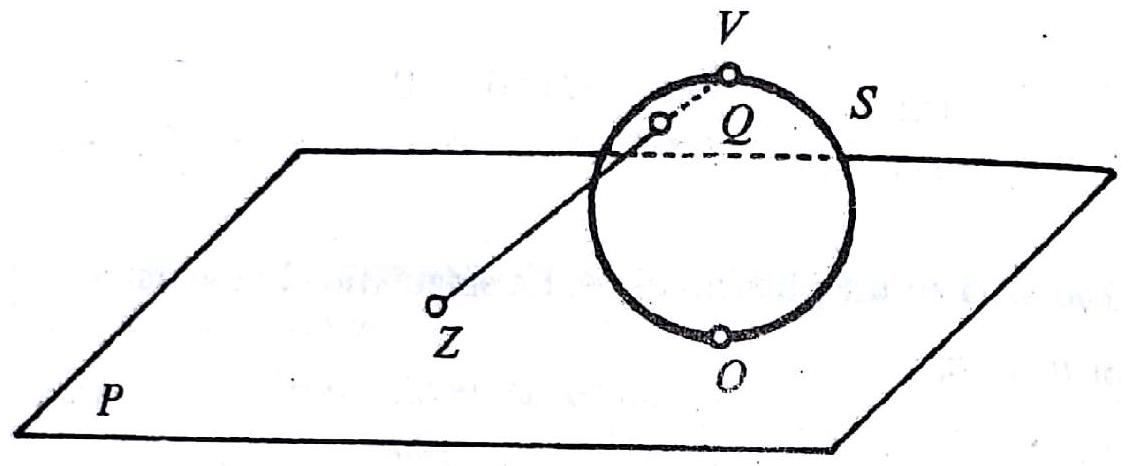
\includegraphics[width=\textwidth]{2025_09_05_adecef5eb2053bc129b5g-085}
\captionsetup{labelformat=empty}
\caption{Figura 6}
\end{center}
\end{figure}

Identifiquemos $P$ con el plano complejo haciendo corresponder el punto 0 a $z=0$. Sea $l$ el extremo opuesto a $O$ del diámetro que une $O$ con el centro de $S$.

Una recta que pase por $l^{\prime}$ y no sea paralela a $P$ corta a $S$ en un punto $Q$ y a $P$ en un punto $z$. La correspondencia $z \rightarrow Q$ aplica biyectiva. mente el plano sobre $S$ desprovisto del punto $V$ y es fácil ver que a un entorno de $z$ en $P$ le corresponde un entorno de $Q$; es decir, un casquete de centro $Q$ en $S$ y recíprocamente.

A un entorno reducido de $l^{\prime}$ en $S$ (es decir, un casquete de centrol' del cual extraemos a $F$ ) esta aplicación hace corresponder el exterior de ull disco de centro () . Luego, si la extendemos haciendo corresponder a l'el punto del infinito, tendremos entre toda la superficie $S$ y el plano complejo más el punto del infinito una aplicación biyectiva que conserva los entornos.

\section{Funciones meromorfas}
\section*{DIAINICION 1:}
Sca $\Omega$ un abierro concero. Lina finncient i: $\Omega \rightarrow$ ( se dice meromert)\\
en $\Omega$ si $\mathrm{z}_{0} \in \Omega$ implica que f es holomorfa en $\mathrm{z}_{0}$ o bien que tiene un polo en $\mathrm{z}_{0}$.

En otros términos $f$ es holomorfa en $\Omega$ salvo en un subconjunto $\Delta \subset \Omega$ en cada punto del cual $f$ tiene un polo. Si $\Delta=\emptyset, f$ es holomorfa en $\Omega$.

\subsection{Ejemplos}
$1^{0}$ ) De acuerdo con lo dicho en el parágrafo anterior, toda función racional es meromorfa en el plano complejo compactificado.\\
$2^{0}$ ) La función ctg $z$ es meromorfa en el plano complejo (sin el punto del $\infty$, que no es una singularidad aislada) pues es holomorfa en todo punto salvo para $z=n \pi$ en donde tiene polos de primer orden.\\
$3^{0}$ ) La función

$$
f(z)=\frac{1}{\operatorname{sen} \frac{1}{z}}
$$

es meromorfa en el dominio

$$
\Omega=\{x+i y \in C: 0<x<1,-1<y<1\}
$$

ya que las únicas singularidades de $f$ son los polos en los puntos $\frac{1}{17 \pi}$.\\
Como vemos en estos ejemplos, una función meromorfa en $\Omega$ puede tener infinitos polos en el dominio, pero esos polos no pueden acumularse en un punto de $\Omega$, ya que en un punto de acumulación de polos no es ni polo ni punto de holomorfismo. Por lo tanto:

\section*{Teoremal}
Si f es meromorja en $\Omega$. $v$ si K es un conjunto cerrado .. acotado contenido en $\Omega$ ea K sölo hay un mimero fiiito de polos.

En efecto, si hubiera una infinidad de ellos, por el teorema de Bolzano-Weierstrass, tendrían un punto de acumulación en $K$ y por lo tanto en $\Omega$. Esto contradice el hecho de que $f$ es meromorfa.

Vamos ahora a caracterizar las funciones meromorjas en el plan() complejo compactificado $v$ veremos que éstas coinciden c'on las funciones racionales.

En efecto, en el parágrafo anterior vimos que una función racional tenía como puntos singulares las raíces del denominador, es decir, un número finito de polos y que el punto del infinito era un polo o una singularidad evitable.

Pasemos ahora a demostrar la recíproca. Sea $f$ meromorfa en el plano compactificado; sean $z_{1} \ldots z_{r}$ los polos de $f$ contenidos en el plano complejo sin el infinito.

En un cierto entorno de $z_{1}, f$ puede escribirse como

$$
f(z)=S_{1}(z)+g_{1}(z)
$$

donde (por el teorema de Laurent) $S_{1}(z)$ es una suma de fracciones simples cuyos denominadores son potencias de $\left(z-z_{1}\right)$ y $g_{1}(z)$ es una función holomorfa en $z_{1}$. Los únicos puntos singulares de $g_{1}(z)$ son $z_{2} \ldots z_{r}$ y eventualmente el infinito. A $g_{1}$ le aplicamos la misma descomposición

$$
g_{1}(z)=S_{2}(z)+g_{2}(z)
$$

donde $S_{2}(z)$ es una suma de potencias negativas de $\left(z-z_{2}\right)$ y $g_{2}(z)$ es una función cuyos puntos singulares son $z_{3} \ldots z_{r}$ y eventualmente el infinito. Reiterando este procedimiento, llegamos a la descomposición

$$
f(z)=\sum_{j=1}^{r} S_{j}(z)+g_{r}(z)=S(z)+g_{r}(z),
$$

donde $S(z)$ es una suma de fracciones simples y $g_{r}(z)$ es una función sin puntos singulares a distancia finita, es decir una función entera. Luego para todo $z \in C$.

$$
g_{r}(z)=\sum_{()}^{\infty} a_{n} z^{n},
$$

pero como el infinito es un polo o una singularidad evitable, este desarrollo sólo puede tener un número finito de términos, es decir, es un polinomio. En consecuencia $f$ es racional, suma de fracciones simples y de un polinomio.

De paso hemos demostrado la posibilidad de descomponer una función racional en fracciones simples.

Si la función fuera holomorfa en todo el plano incluyendo el punto del infinito, debería ser constante.

En efecto: por ser holomorfa admite un desarrollo en serie

$$
f(z)=\sum_{0}^{\infty} a_{n} z^{n}
$$

convergente para todo $z$. Como $f$ es además holomorfa en el infinito, no puede tener potencia de exponente $\geqslant 1$, es decir $f(z)=a_{0}$, como quería mos demostrar.

\section{Residuos}
\section*{DEFINICION 1:}
Sea funa función holomorfa en un disco D reducido: $0<\left|z-z_{0}\right| \leqslant \mathrm{R}$ Se denomina residuo de f en $\mathrm{z}_0 y$ se indica $\mathrm{R}\left[\mathrm{f}, \mathrm{z}_0\right]$ al coeficiente del término en $\left(\mathrm{z}-\mathrm{z}_0\right)^{-1}$ del desarrollo en serie de Laurent de f en D ; es decir:


\begin{equation*}
R\left[f, z_{0}\right]=a_{-1}=\frac{1}{2 \pi i} \int_{\Gamma^{+}} f(z) d z \tag{20-1}
\end{equation*}


siendo $\Gamma^{+}$una circunferencia de centro $z_{0}$ contenida en el disco $D$ y recorrida en el sentido positivo.

Naturalmente, si la función es holomorfa en $z_{0}$ el residuo es cero. Este caso trivial carece de interés y en general cuando se habla de residuo de una función en un punto, se supone que el mismo es singular aislado con singularidad no evitable. El residuo puede ser nulo en un punto en el que la función no es holomorfa. Por ejemplo

$$
R\left[\frac{1}{z^{2}}, 0\right]=0
$$

El interés de este concepto radica en la posibilidad de calcularlo directamente (por derivaciones, paso al límite u otros procedimientos) y después utilizarlo para calcular integrales.

Mostraremos con ejemplos cómo es posible hallar algunos residuos.\\
$1^{0}$ ) Sea $f_{1}(z)=\frac{1}{z^{2}(z+1)}$.

Esta función tiene un polo doble en $z=0$ y un polo simple en $z=-1$. Para llegar al desarrollo de Laurent de $f_{1}$ alrededor de esos puntos, comen. zaremos por descomponer nuestra función racional en suma de fracciones simples.

Luego\\
$\frac{1}{z^{2}(z+1)}=\frac{A}{z}+\frac{B}{z^{2}}+\frac{C}{z+1} \Longrightarrow\left\{\begin{aligned} A+C & =0 \\ A+B & =0 \\ B & =1\end{aligned} \Longrightarrow\left\{\begin{array}{c}A=-1 \\ B=1 \\ C=1\end{array}\right.\right.$\\
y $\frac{1}{z^{2}(z+1)}=\frac{1}{z^{2}}-\frac{1}{z}+\frac{1}{z+1}$\\
Como

$$
\frac{1}{z+1}=1-z+\cdots+(-1)^{n} z^{n}+\cdots
$$

es holomorfa en $z=0$, el desarrollo de Laurent de $f_{1}$ en el entorno de cero es

$$
\frac{1}{z^{2}}-\frac{1}{z}+1-z+z^{2}+\cdots
$$

Análogamente, el desarrollo de $f_{1}$ en serie de Laurent en un entorn 0 de $z=-1$ es de la forma

$$
\frac{1}{z+1}+a_{0}+a_{1}(z+1)+\cdots+a_{n}(z+1)^{n}+\cdots
$$

y por lo tanto por simple inspección

$$
R\left[f_{1}, 0\right]=-1 \quad ; \quad R\left[f_{1},-1\right]=1 .
$$

$2^{0}$ ) Sea

$$
f_{2}(z)=\frac{1}{z^{3}} \operatorname{sen} z
$$

La única singularidad en el plano complejo está en $z=0$.\\
El desarrollo de Laurent alrededor de esa singularidad es

$$
\frac{1}{z^{3}}\left(z-\frac{z^{3}}{3!}+\cdots\right)=\frac{1}{z^{2}}-\frac{1}{6}+\cdots
$$

luego el 0 es un polo doble y $R\left[f_{2}, 0\right]=0$.\\
$3^{0}$ ) Sea $f_{3}(z)=z^{5} \cos \frac{1}{z}$\\
El desarrollo en serie de Laurent alrededor de la singularidad $z=0$ es

$$
\begin{gathered}
z^{5}\left(1-\frac{1}{2!z^{2}}+\frac{1}{4!z^{4}}-\frac{1}{6!z^{6}}+\cdots+\frac{(-1)^{n}}{(2 n)!z^{2 n}}+\cdots\right)= \\
=z^{5}-\frac{1}{2!} z^{3}+\frac{1}{4!} z-\frac{1}{6!} \frac{1}{z}+\frac{1}{8!} \frac{1}{z^{3}}-\cdots
\end{gathered}
$$

Luego la singularidad es esencial y $\quad R\left[f_{3}, 0\right]=\frac{-1}{720}$.\\
$4^{0}$ ) Sea $f_{4}(z)=\frac{1}{1+z} e^{1 / z}$.

Las singularidades son $z=0$ y $z=-1$.\\
En $0<|z|<1$ el desarrollo en serie de Laurent puede obtenerse multiplicando los desarrollos en serie de ambos factores:

$$
\left[1-z+z^{2}+\cdots+(-1)^{n} z^{n}+\cdots\right]\left[1+\frac{1}{z}+\cdots+\frac{1}{m!} \frac{1}{z^{m}}+\cdots\right]
$$

El coeficiente de $z^{-1}$ en este desarrollo será la suma de los productos del coeficiente de $z^{k}$ en el primer factor por el de $z^{-(k+1)}$ en el segundo, es decir,

$$
R\left[f_{4}, 0\right]=\sum_{k=0}^{\infty} \frac{(-1)^{k}}{(k+1)!}=1-\frac{1}{2!}+\frac{1}{3!}-\ldots
$$

y como

$$
\begin{gathered}
e^{-1}=1-\frac{1}{1!}+\frac{1}{2!}-\frac{1}{3!}+\cdots=\frac{1}{2!}-\frac{1}{3!}+\cdots \\
1-e^{-1}=R\left[f_{4}, 0\right]
\end{gathered}
$$

En $0<|z+1|<1$, la función $e^{1 / z}$ admite un desarrollo en serie de potencias positivas cuyo término independiente es el valor de $e^{1 / 2}$ en $z=-1$, es decir $e^{-1}$. Luego

$$
\frac{1}{z+1}\left[e^{-1}+a_{1}(z+1)+a_{2}(z+1)^{2}+\cdots\right]
$$

y entonces

$$
R\left[f_{4},-1\right]=\frac{1}{e}
$$

Daremos ahora la regla general para el cálculo de los residuos en el caso de un polo.\\
exactamente el mismo número de raices contada cada una tantas veces como su orden de multiplicidad.

En efecto:

$$
f(z)+g(z)=f(z)\left[1+\frac{g(z)}{f(z)}\right]
$$

Luego


\begin{equation*}
\arg \{f(z)+g(z)\}=\arg f(z)+\arg \left[1+\frac{g(z)}{f(z)}\right] \tag{25-3}
\end{equation*}


pero como

$$
\left|\frac{g(z)}{f(z)}\right|<1
$$

el punto

$$
1+\frac{g(z)}{f(z)}
$$

está siempre dentro del disco $|z-1|<1$ y por lo tanto no puede dar ninguna vuelta alrededor del origen, en consecuencia la variación del argumento de

$$
\left[1+\frac{g(z)}{f(\dot{z})}\right]
$$

es nula cuando $z$ describe $\Gamma$.\\
Como de (25-3) se tiene

$$
V_{\Gamma}[\arg \{f(z)+g(z)\}]=V_{\Gamma}[\arg \{f(z)\}]+V_{\Gamma}\left[\arg \left\{1+\frac{g(z)}{f(z)}\right\}\right]
$$

resulta que la variación del argumento de $[f+g]$ coincide con la del\\
argumento de $f$ sobre l'. Por hipótesis, $f$ y $g$ carecen de polos sobre $\Omega$; aplicando (25-2) cl teorema queda demostrado.

Aplicaremos este teorema para obtener una nueva demostración del teorema fundamental del álgebra sobre existencia de raíces de los polj. nomios.

Si $P(z)=a_{n} z^{n}+\cdots+a_{1} z+a_{0}$ es un polinomio de grado $n$, se consideran los polinomios

$$
f(z)=a_{n} z^{n} ; g(z)=a_{n-1} z^{n-1}+a_{n-2} z^{n-2}+\cdots+a_{0},
$$

tales que $P(z)=f(z)+g(z)$. Para $|z| \rightarrow \infty$, el cociente de $g$ por $f$ tiende a 0 . Luego podemos encontrar un $R>0$ tal que para $|z|=R$

$$
|f(z)|>|g(z)|>0
$$

Luego $f, g$ satisfacen las hipótesis del teorema de Rouché. Para $|z|<R$, $f$ tiene una sola raíz de orden $n$, luego $P=f+g$ tiene $n$ raíces. en ese dominio.

\section{Funciones expresables en función del logaritmo}
Si $\alpha \in C$, la función potencial $z^{a}$ queda definida mediante la fórmula

$$
z^{a}=e^{a \log z}=e^{a \log |z|} e^{a i \arg z}=e^{a \log |z|} e^{a i[\arg z+2 K \pi]} .(26-1)
$$

Si fijamos un dominio simplemente conexo que no contenga al origen, para cada $K$ entero tendremos una determinación $\varphi_{K}$ de la función potencial

$$
\varphi_{K}(z)=e^{\left.a \log \right|_{z} \mid} e^{a i \arg z} e^{2 K a \pi i}
$$

Dos de estas determinaciones, $\varphi_{n}$ y $\varphi_{m}$, serán iguales si, y sólo si

$$
e^{2 n a \pi i}=e^{2 m a \pi i} \Leftrightarrow e^{2(n-m) a \pi i}=1 \Longleftrightarrow(n-m) \alpha \text { es un entero. }
$$

Luego si $\alpha$ es un entero, como era de esperar, todas las determinaciones son iguales.

Si $\alpha$ no es racional, todas las determinaciones son distintas. Si, en cambio, $\alpha$ es un número racional no entero, es decir, de la forma $p / q$ con $p$ y $q$ primos entre sí, para que las determinaciones $\varphi_{n}$ y $\varphi_{m}$ coincidan debe ser $(m-n) p$ múltiplo de $q$. Esto equivale, ya que $p$ y $q$ no tienen divisores comunes, a que ( $m-n$ ) sea múltiplo de $q$. Luego, fijado un entero $m$, la determinación $\varphi_{n}$ será idéntica a la $\varphi_{m}$ si, y sólo si, $m$ y $n$ son congruentes módulo $q$. Por ello, habrá tantas determinaciones distintas como clases de congruencia módulo $q$.

A partir de una determinación $\varphi_{0}$ dada, todas las otras se expresan como

$$
\varphi_{k}(z)=\varphi_{0}(z) e^{\frac{2 k \pi i}{q}} \quad \text { para } k=1, \ldots, q-1
$$

Como era de esperar se obtienen las $q$ determinaciones de $\sqrt[q]{z p}$.\\
Vemos por lo tanto que, con excepción del caso en que $\alpha$ es entero, la función $f(z)=z^{a}$ tiene un punto de ramificación en el origen.

La derivada de una determinación de $z^{a}$ (naturalmente definida en un dominio simplemente conexo que no contiene al origen) es

$$
\frac{d}{d z}\left(z^{a}\right)=\frac{d}{d z}\left(e^{a \log z}\right)=e^{a \log z} \frac{\alpha}{z}=z^{a} \frac{\alpha}{z}=\alpha z^{a-1}
$$

Como las funciones trigonométricas son combinaciones de exponenciales, sus inversas pueden expresarse en términos del logaritmo. Veamos por ejemplo el caso de la función arc $\operatorname{tg} z$ : Si $w=\operatorname{arc} \operatorname{tg} z$, se tiene:

$$
z=\operatorname{tg} w=\frac{1}{i} \frac{e^{i w}-e^{-i w}}{e^{i w}+e^{-i w}}=\frac{1}{i} \frac{e^{2 i w}-1}{e^{2 i w}+1}
$$

Operando:

$$
\begin{aligned}
& i z e^{2 i w}+i z=e^{2 i w}-1 \\
& e^{2 i w}(1-i z)=1+i z \\
& e^{2 i w}=\frac{1+i z}{1-i z}=\frac{i-z}{i+z} \\
& w=\operatorname{arctg} z=\frac{1}{2 i} \log \frac{i-z}{i+z}
\end{aligned}
$$

Como

$$
\log \frac{i-z}{i+z}=\log \left|\frac{i-z}{i+z}\right|+i \arg \left(\frac{i-z}{i+z}\right),
$$

la función $w=\operatorname{arc} \operatorname{tg} z$ tiene infinitas determinaciones.\\
Además, $z=-i$ y $z=i$ son puntos de ramificación de $w$, ya que corresponden a los puntos $z=\infty, z=0$ de ramificación del logaritmo.\\
27. Cálculo de integrales con logaritmos y potencias no enteras

Veamos una manera de calcular las integrales de la forma

$$
I=\int_{0}^{\infty} \frac{f(x)}{x^{a}} d x
$$

donde $\alpha$ es un número real tal que $0<\alpha<1$ y

$$
f(x)=\frac{P(x)}{Q(x)}
$$

es una función racional tal que su denominador $Q$ no tiene ninguna raíz positiva y su grado es mayor que el grado de $P$.

La integral es convergente:\\
En efecto, como el integrando es continuo sobre todo intervalo finito que no contenga al origen, bastará analizar la integral alrededor del cero y del infinito.

En un entomo de cero la función $f(x)$ está acotada y al ser $\alpha<1$ el integrando crece como una potencia de exponente $-\alpha>-1$, que es integrable.

Si llamamos $k=$ grado $Q-$ grado $P$, es $k \geqslant 1$. Luego, en un entorno del infinito, $f(x)$ decrece como $x^{-k}$ con $k \geqslant 1$ y en consecuencia el integrando se comporta como $x^{-k-a}$, con $k+\alpha<1$, que es integrable en el infinito.

Consideremos el siguiente camino de integración:

\begin{figure}[h]
\begin{center}
  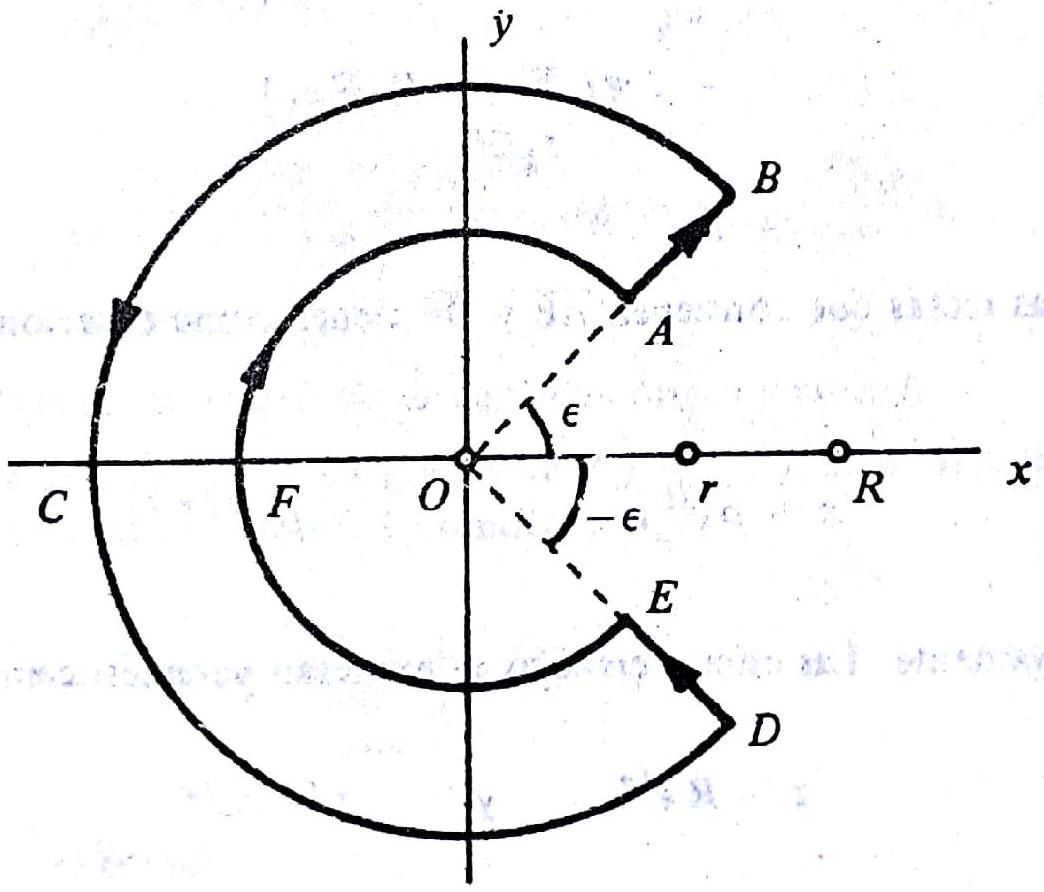
\includegraphics[width=\textwidth]{2025_09_05_adecef5eb2053bc129b5g-096}
\captionsetup{labelformat=empty}
\caption{Figura 13}
\end{center}
\end{figure}

donde $r$ y $R$ son dos reales positivos, $0<r<R$ tales que todas las raíces de $Q$ estén en el interior de la corona $r<|z|<R$.

El contorno está constituido por los arcos $\widehat{\mathrm{BCD}}$, de radio $R$ y $\widehat{\mathrm{EFA}}$ de radio $r$, y por los segmentos $\overline{A B}$ y $\overline{D E}$ ubicados sobre los radios vectores $\arg z=\varepsilon$ y $\arg z=2 \pi-\varepsilon$, respectivamente.

El dominio $D$ limitado por ese contorno es un conjunto simplemente conexo que no contiene al origen. Por to tanto en él puede definirse la determinación de $x^{a}$ correspondiente al argumento de $z: 0 \leqslant \arg z<2 \pi$.

Para $r, \in$ y $R$ adecuados, el dominio $D$ contendrá todas las singularidades de la función $f$. Sea

$$
F(z)=\frac{f^{\prime}(z)}{z^{a}} .
$$

Luego, aplicando el teorema de los residuos,

$$
\int_{\widehat{\mathrm{AB}}} F(z) d z+\int_{\widehat{\mathrm{BCD}}} F(z) d z+\int_{\widehat{\mathrm{DE}}} F(z) d z+\int_{\widehat{\mathrm{EFA}}} F(z) d z=
$$


\begin{equation*}
=2 \pi i \sum_{z_{k} \in D} R\left[F, z_{k}\right] . \tag{27.1}
\end{equation*}


Las rectas que contienen $\overline{\mathrm{AB}}$ y $\overline{\mathrm{DE}}$ tienen como ecuaciones paramétricas

$$
z=\rho e^{i \varepsilon} \quad y \quad z=\rho e^{i(2 \pi-\varepsilon)}
$$

respectivamente. Las circunferencias se expresan paramétricamente como

$$
z=R e^{i \varphi} \quad y \quad z=r e^{i \varphi} .
$$

Se tiene entonces

$$
\int_{\overline{\mathrm{AB}}} F(z) d z=\int_{r} R \frac{f\left(\rho e^{i \epsilon}\right)}{\rho^{a} e^{i a \xi}} e^{i \xi} d \rho \xrightarrow[\xi \rightarrow 0]{ } \int_{r}^{R} \frac{f(\rho)}{\rho^{a}} d \rho
$$

que a su vez tiende hacia la integral buscada $l$, cuando $r \rightarrow 0$ y $R \rightarrow \infty$.

Además

$$
\int_{\overline{\mathrm{DE}}} F(z) d z=-\int_{r}^{R} \frac{f\left[\rho e^{i(2 \pi-\varepsilon)}\right]}{\rho^{a} e^{i a(2 \pi-\varepsilon)}} e^{i(2 \pi-\varepsilon)} d \rho
$$

Si $\varepsilon \rightarrow 0$ la integral tiende hacia

$$
-e^{-2 \pi i a} \int_{r}^{R} \frac{f(\rho)}{\rho^{a}} d \rho
$$

la que a su vez tiende hacia - $e^{-2 \pi i a} I$ para $r \rightarrow 0$ y $R \rightarrow \infty$.\\
La integral sobre el arco de circunferencia de radio $R$ es

$$
\begin{gathered}
\int_{\widehat{\mathrm{BCD}}} F(z) d z=\int_{\varepsilon}^{2 \pi-\varepsilon} \frac{f\left(R e^{i \varphi}\right) i R e^{i \varphi}}{R^{a} e^{i a \varphi}} d \varphi \\
\underset{\varepsilon \rightarrow 0}{\longrightarrow} \int_{0}^{2 \pi} \frac{f\left(R e^{i \varphi}\right) i R e^{i \varphi}}{R^{a} e^{i a \varphi}} d \varphi=\int_{\Gamma^{\prime}(R)} \frac{f(z)}{z^{a}} d z
\end{gathered}
$$

donde $\Gamma(R)$ es la circunferencia de centro el origen y radio $R$.\\
Por la relación entre los grados de $P$ y $Q,|z f(z)|$ es acotada en un entorno del punto del infinito; y como $\alpha>0$, es

$$
\lim _{z \rightarrow \infty}\left|z \frac{f(z)}{z^{\alpha}}\right|=0
$$

Entonces como

$$
\left|\int_{\Gamma(R)} \frac{f(z)}{z^{a}} d z\right| \leqslant 2 \pi R \sup _{z \in \Gamma(R)}\left|\frac{f(z)}{z^{a}}\right|=2 \pi \sup _{z \in \Gamma(R)}\left|\frac{z f(z)}{z^{\infty}}\right|
$$

la integral sobre el arco $\widehat{\mathrm{BCD}}$ tiende a cero cuando $R \rightarrow \infty$ y $\varepsilon \rightarrow 0$.\\
Un razonamiento análogo prueba que la integral sobre AFE tiende a cero cuando $\varepsilon$ y $r$ tienden a.cero.

Por lo tanto, pasando al límite en (27-1) para $\varepsilon \rightarrow 0, R \rightarrow \infty y r \rightarrow 0$ se obtiene


\begin{equation*}
\left(1-e^{-2 \pi i a}\right) I=2 \pi i \Sigma \operatorname{Res}\left[\frac{f(z)}{z^{a}}, z_{k}\right] \tag{27-2}
\end{equation*}


que nos da el valor de la integral.

\section*{Ejemplo}
Calculemos la integral

$$
I=\int_{0}^{\infty} \frac{\sqrt[3]{x} d x}{1+x^{2}}
$$

que es del tipo anterior, ya que el integrando puede ponerse en la forma

$$
\frac{\sqrt[3]{x}}{1+x^{2}}=\frac{x}{\left(1+x^{2}\right) x^{2 / 3}}
$$

siendo el exponente $\alpha=2 / 3$ y los puntos singulares $z=i$ y $z=-i$.\\
Luego teniendo en cuenta (27-2) se obtiene:

$$
I\left(1-e^{-\frac{4 \pi l}{3}}\right)=2 \pi i\left\{R\left[\frac{z^{1 / 3}}{1+z^{2}}, i\right]+R\left[\frac{z^{1 / 3}}{1+z^{2}},-i\right]\right\}
$$

El primer residuo vale

$$
\frac{i^{1 / 3}}{2 i}
$$

mientras que el segundo es

$$
\frac{(-i)^{1 / 3}}{-2 i} .
$$

Hay que precisar cuál de las tres determinaciones de la raíz cúbica\\
es la adecuada. Hemos tomado como valor de argumento $z$ al que para $z=i$ vale $\pi / 2$. Por lo tanto la raíz cúbica correspondiente es

$$
e^{\frac{\pi i}{6}}=\frac{\sqrt{3}}{2}+i \frac{1}{2} .
$$

Para $z=-i$, el argumento a considerar es $3 \pi / 2$ y la raíz cúbica correspondiente es

$$
e^{\frac{\pi}{2} i}=i
$$

Por otra partes es

$$
\begin{aligned}
1-e^{-\frac{4 \pi i}{3}} & =1-e^{-\frac{4 \pi i}{3}} e^{2 \pi i}=1-e^{\frac{2 \pi i}{3}}=1-\left(-\frac{1}{2}+\frac{i \sqrt{3}}{2}\right)= \\
& =\frac{3-i \sqrt{3}}{2}
\end{aligned}
$$

Simplificando el factor $2 i$, se tiene

$$
I=\frac{2 \pi}{3-i \sqrt{3}}\left(\frac{\sqrt{3}}{2}+\frac{i}{2}-i\right)=\frac{\pi(\sqrt{3}-i)}{3-i \sqrt{3}}=\frac{\pi}{\sqrt{3}}
$$

El procedimiento de cálculo anterior puede simplificarse cuando la fuñción $f$, además de cumplir con las condiciones fijadas, es par o impar.

Veámoslo tomando el contorno de integración formado por el seg. mento $[r, R]$ del cje real, la semicircunferencia de centro $O$ y radio $R$ situado en el semiplano superior; el segmento $[-R,-r]$ del eje real y la semicircunferencia de centro $O$ y radio $r$ situado en el semiplano superior.

La semicorona limitada por ese contorno es un dominio $\Omega$ simplemente conexo que no contiene al origen. En él puede definirse una determinación de $z^{a}$ correspondiente al argumento: $0 \leqslant \arg z<2 \pi$.

\begin{figure}[h]
\begin{center}
  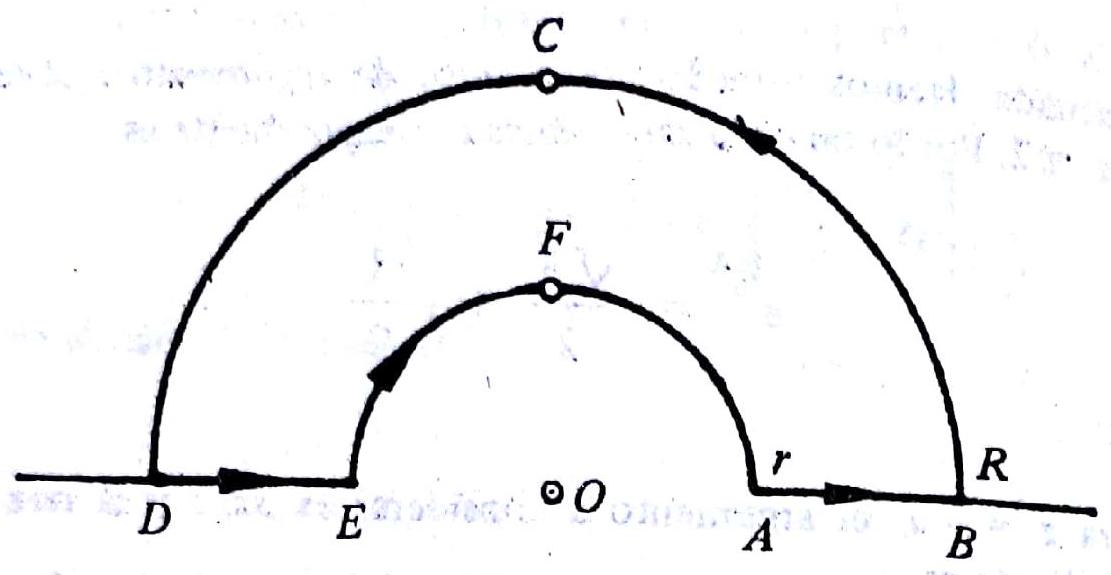
\includegraphics[width=\textwidth]{2025_09_05_adecef5eb2053bc129b5g-101}
\captionsetup{labelformat=empty}
\caption{Figura 14}
\end{center}
\end{figure}

Supongamos además que $\Omega$ contiene a todos los polos de la función $f$ en el semiplano superior. Si llamamos

$$
F(z)=\frac{f(z)}{z^{a}}
$$

y aplicamos el teorema de los residuos, se tendrá

$$
\begin{aligned}
\int_{\overline{\mathrm{AB}}} F(z) d z+\int_{\overline{\mathrm{BCD}}} F(z) d z+\int_{\overline{\mathrm{DE}}} F(z) d z+\int_{\overline{\mathrm{EFA}}} F(z) d z= & \\
= & 2 \pi i \sum_{\operatorname{Im} z_{k}>0} R\left[F, z_{k}\right]
\end{aligned}
$$

Imitando lo hecho en el caso anterior, podriamos probar que la segunda y la cuarta integral tienden a cero para $R \rightarrow \infty$ y para $r \rightarrow 0$ respectivamente.

Análogamente, la primera tiende a $I$ cuando $R \rightarrow \infty$ y $r \rightarrow 0$.\\
Veamos entonces qué sucede con la tercera.\\
La ecuación del segmento $\overline{\mathrm{DE}}$ es $z=\rho e^{i \pi}$ para $\rho$ comprendido entre $r$ y $R$. Luego

$$
\int_{\overline{\mathrm{DE}}} F(z) d z=-\int_{r}^{R} \frac{f\left(\rho e^{i \pi}\right) e^{i \pi}}{\rho^{a} e^{i \pi a}} d \rho=c^{-i \pi a} \int_{r}^{R} \frac{f(\cdot \rho)}{\rho^{a}} d \varphi
$$

Si $f$ es par es $f(\rho)=f(-\rho)$ mientras que síf es impar $f(-\rho)=-j(\rho)$.

Luego

$$
\lim _{\substack{r \rightarrow 0 \\ R \rightarrow \infty}} \int_{\overline{\mathrm{DE}}} F(z) d z= \pm e^{-i \pi a}
$$

y, por lo tanto, se deduce


\begin{equation*}
\left(1 \pm e^{-i \pi a}\right) I=2 \pi i \sum_{I m z_{k}>0} R\left[\frac{f(z)}{z^{a}}, z_{k}\right] \tag{27-3}
\end{equation*}


el doble signo del primer miembro debe entenderse como + si $f$ es par, y como - si $f$ és impar.

Naturalmente, la ventaja de este procedimiento reside en que sólo es necesario calcular los residuos en los polos del semiplano superior.

\section*{Ejemplo}
Calculemos

$$
I=\int_{0}^{\infty} \frac{\sqrt[3]{x}}{\left(1+x^{2}\right)^{2}} d x
$$

Como se puede poner el integrando en la forma

$$
\frac{x}{\left(1+x^{2}\right)^{2}} \frac{1}{x^{2 / 3}}
$$

estamos en las condiciones de aplicación de (27-3), con $\alpha=2 / 3$ y función impar. Luego

$$
\left(1-e^{-\frac{2 \pi}{3} i}\right) I=2 \pi i R\left[\frac{z^{1 / 3}}{\left(1+z^{2}\right)^{2}}, i\right] .
$$

El coeficiente del primer miembro es

$$
1-e^{-\frac{2 \pi}{3} i}=1-\left(-\frac{1}{2}-i \frac{\sqrt{3}}{2}\right)=\frac{3+i \sqrt{3}}{2},
$$

mientras que para calcular el residuo en el polo doble $z=i$, consideremos la función

$$
g(z)=(z-i)^{2} \frac{z^{1 / 3}}{\left(z^{2}+1\right)^{2}}=\frac{z^{1 / 3}}{(z+i)^{2}} .
$$

Para ella es\\
$g^{\prime}(z)=\frac{1}{3} z^{-2 / 3}(z+i)^{-2}-z^{1 / 3} 2(z+i)^{-3}=z^{1 / 3}(z+i)^{-2}\left[\frac{1}{3 z}-\frac{2}{z+i}\right]$\\
y como

$$
g^{\prime}(i)=R\left[\frac{z^{1 / 3}}{\left(1+z^{2}\right)^{2}}, i\right] ;
$$

éste vale

$$
i^{1 / 3}\left(\frac{-1}{4}\right)\left[\frac{1}{3 i}-\frac{1}{i}\right]=\frac{i^{1 / 3}}{6 i}=\frac{1}{12 i}(\sqrt{3}+i) .
$$

La integral vale\\
$I=\frac{2}{3+i \sqrt{3}} 2 \pi i \frac{1}{12 i}(\sqrt{3}+i)=\frac{\pi}{3} \frac{\sqrt{3}+i}{3+i \sqrt{3}}=\frac{\pi}{3 \sqrt{3}}$.

Calculemos ahora integrales de la forma


\begin{equation*}
I=\int_{0}^{\infty} f(x) \log x d x \tag{$(27.4$}
\end{equation*}


en las que

$$
f(x)=\frac{P(x)}{Q(x)}
$$

es una función racional cociente de dos polinomios $P$ y $Q$ tales que el grado de $P$ es inferior al menos en dos unidades al grado de $Q$ y éste no tiene ninguna raíz real mayor o igual que cero.

La integral es convergente:\\
Descomponiendo como antes el rango de integración en los intervalos $(0 a),[a, b]$ y $(b,+\infty)$, la continuidad del integrando nos asegura la convergencia en el segundo de ellos.

Al estar $f(x)$ acotada en un entorno de $x=0$, el integrando crece coino el logaritmo, y como

$$
\int_{0}^{a} \log x d x<\infty
$$

podemos asegurar también la convergencia en el primero de los intervalos.\\
Si aliora llamamos $k=$ grado de $Q$ - grado de $P$ y observamos que $k \geqslant 2$, vemos que la integral de $f(x) \log x$ sobre ( $b, \infty$ ) se comporta como la

$$
\int_{b^{\prime}}^{+\infty} x^{-k} \log x d x
$$

que es convergente.\\
Consideremos nuevamente el dominio $D$ que utilizamos para el cálculo de la integral de $f(x) / x^{a}$. (Fig. 13).

Determinemos el logaritmo utilizando el argumento principal

$$
0 \leqslant \arg z<2 \pi
$$

Determinemos $r, R$ y $\epsilon$ mayores que cero y tales que en $D$ estén todos los polos de la función $f(z)$, apliquemos el teorema de los residuos a la función.

$$
F(z)=(\log z)^{2} \cdot f(z)
$$

resulta:


\begin{gather*}
\int_{\widehat{\mathrm{AB}}} F(z) d z+\int_{\widehat{\mathrm{BCD}}} F(z) d z+\int_{\widehat{\mathrm{DE}}} F(z) d z+\int_{\widehat{\mathrm{EFA}}} F(z) d z= \\
=2 \pi i \sum R\left[F, z_{k}\right] \tag{27.5}
\end{gather*}


Se tiene

$$
\int_{\overline{\mathrm{AB}}} F(z) d z=\int_{r}^{R} f\left(\rho e^{i \xi}\right)\left[\log \left(\rho e^{i \varepsilon}\right)\right]^{2} e^{i \varepsilon} d \rho,
$$

luego

$$
\lim _{\varepsilon \rightarrow 0} \int_{\overline{\mathrm{AB}}} F(z) d z=\int_{r}^{R} f(\rho)[\log \rho]^{2} d \rho
$$

la que para $r \rightarrow 0$ y $R \rightarrow \infty$ tiende hacia

$$
I_{2}=\int_{0}^{\infty} f(x)(\log x)^{2} d x
$$

La tercera integral es

$$
\begin{aligned}
\int_{\overline{\mathrm{DE}}} F(z) d z & =-\int_{r}^{R} f\left(\rho e^{i(2 \pi-\varepsilon)}\right) \cdot\left[\log \rho e^{i(2 \pi-\varepsilon)}\right]^{2} e^{i(2 \pi-\varepsilon)} d \rho= \\
& =-\int_{r}^{R} f\left(\rho e^{i(2 \pi-\varepsilon)}\right) \cdot[\log \rho+i(2 \pi-\varepsilon)]^{2} e^{i(2 \pi-\varepsilon)} d \rho_{1}
\end{aligned}
$$

la que para $\varepsilon \rightarrow 0$ tiende hacia

$$
-\int_{r}^{R} f(\rho)[\log \rho+2 \pi i]^{2} d \rho
$$

Esta integral, a su vez, para $r \rightarrow 0$ y $R \rightarrow \infty$ tiende hacia\\
$-\int_{0}^{\infty} f(\rho)(\log \rho)^{2} d \rho-4 \pi i \int_{0}^{\infty} f(\rho) \log \rho d \rho+4 \pi^{2} \int_{0}^{\infty} f(\rho) d \rho$.

Llamando $I_{0}$ a la

$$
\int_{0}^{\infty} f(x) d x, \quad \text { la } \quad \int_{\overline{\mathrm{DE}}} F(z) d z
$$

tiende entonces hacia

$$
-I_{2}-4 \pi i I+4 \pi^{2} I_{0} .
$$

La integral sobre la circunferencia de radio $R$ tiende a cero para $\varepsilon \rightarrow 0$ y $R \rightarrow \infty$ y la integral sobre la circunferencia pequeña de radio $r$ tiende igualmente a cero para $\varepsilon \rightarrow 0$ y $r \rightarrow 0$. Tomando límites en (27-5) resulta:\\
$2 \pi i \sum R\left[F(z), z_{k}\right]=\lim _{\substack{z \rightarrow 0 \\ r \rightarrow 0 \\ R \rightarrow \infty}} \int_{A B C D E F A} F(z) d z=$

$$
=I_{2}+\left(-I_{2}-4 \pi i I+4 \pi^{2} I_{0}\right)=-4 \pi i I+4 \pi^{2} I_{0} .
$$

Simplificando, queda

$$
I+\pi i I_{0}=-\frac{1}{2} \sum R\left[F(z), z_{k}\right],
$$

y tomando parte real y parte imaginaria se obtienen las formulas finales:


\begin{equation*}
I=-\frac{1}{2} R e\left\{\Sigma R\left[f(z)(\log z)^{2}, z_{k}\right]\right\} \tag{27-6}
\end{equation*}



\begin{equation*}
I_{0}=-\frac{1}{2 \pi} \operatorname{Im}\left\{\Sigma R\left[f(z)(\log z)^{2}, z_{k}\right]\right\} \tag{27.7}
\end{equation*}


\section*{Ejemplo}
Calculemos la integral

$$
\int_{0}^{\infty} \frac{\log x}{(1+z)^{3}} d x
$$

utilizando (27-6):\\
Empezaremos por determinar el residuo de

$$
F(z)=\frac{(\log z)^{2}}{(1+z)^{3}}
$$

en el polo triple $z=-1$. Llamando $g(z)=F(z)(1+z)^{3}(\log z)^{2}$ se tiene

$$
g^{\prime}(z)=\frac{2 \log z}{z} \text { y } \quad g^{\prime \prime}(z)=2 z^{-2}-2 \log z z^{-2}=\frac{2(1-\log z)}{z^{2}}
$$

Entonces,

$$
R[F(z),-1]=\frac{1}{2} g^{\prime \prime}(-1)=1-\log (-1)=1-\pi i
$$

Aplicando (27-6) y (27-7) se obtiene

$$
I=\int_{0}^{\infty} \frac{\log x}{(1+x)^{3}} d x=-\frac{1}{2} \quad \text { e } \quad I_{0}=\int_{0}^{\infty} \frac{d x}{\left(1+x^{3}\right)}=\frac{1}{2}
$$

El cálculo puede simplificarse cuando $f$ es una función par (aunque\\
no si $f$ es impar), tomando el contorno del dominio $\Omega$ estudiado antes y aplicando el teorema de los residuos directamente esta vez a la función,

$$
F(z)=f(z) \log z .
$$

Tendríamos entonces (fig. 14):

$$
\begin{gathered}
\int_{\overline{\mathrm{AB}}} F(z) d z+\int_{\widehat{\mathrm{BCD}}} F(z) d z+\int_{\overline{\mathrm{DE}}} F(z) d z+\int_{\widehat{\mathrm{EFA}}} F(z) d z= \\
=2 \pi i \sum_{\operatorname{Im} z_{k}>0} R\left[F, z_{k}\right]
\end{gathered}
$$

La segunda integral tiende a cero para $R \rightarrow \infty$, la cuarta tiende a cero para $r \rightarrow 0$. La primera tiende a la integral pedida para $R \rightarrow \infty$ y $r \rightarrow 0$. Calculemos entonces la tercera.

La ecuación de la recta que contiene al segmento $\overline{\mathrm{DE}}$ es $z=\rho e^{i \pi}$. Luego

$$
\begin{gathered}
\int_{\mathrm{DE}} F(z) d z=-\int_{r}^{R} f\left(\rho e^{i \pi}\right)(\log \rho+i \pi) e^{i \pi} d \rho= \\
=\int_{r}^{R} f(-\rho) \log \rho d \rho+\pi i \int_{r}^{R} f(-\rho) d \rho
\end{gathered}
$$

Como $f$ es par, para $r \rightarrow 0$ y $R \rightarrow \infty$ la integral sobre $\overline{\mathrm{DE}}$ tiende hacia $I+i \pi I_{0}$. Luego:

$$
2 I+\pi i I_{0}=2 \pi i \sum_{\operatorname{Im} z_{k}>0} R_{r}\left[f(z) \log z_{z} z_{k}\right]
$$

o bien:

$$
\frac{1}{2} I_{0}-\frac{i}{\pi} I=\sum_{\operatorname{Im} z_{k}>0} R\left[f(z) \log z_{,} z_{k}\right] .
$$

Tomando partes real e imaginaria


\begin{align*}
\int_{0}^{\infty} f(x) \log x d x & =-\pi \operatorname{Im}\left\{\sum_{\mid m, z_{k}>0} R\left[f(z) \log z, z_{k}\right]\right\} ;  \tag{$27\cdot8$}\\
\int_{0}^{\infty} f(x) d x & =-\operatorname{Re}\left\{\sum_{I m, z_{k}>0} R\left[f(z) \log z, z_{k}\right]\right\} \tag{27-9}
\end{align*}


Por ejemplo, calculemos:

$$
I=\int_{0}^{\infty} \frac{\log x}{1+x^{2}} d x
$$

El residuo en el punto $i$ es:

$$
\left|\frac{\log z}{2 z}\right|_{z=i}=\frac{\log i}{2 i}=\frac{1}{2 i} \frac{\pi}{2} i=\frac{\pi}{4}
$$

Y de acuerdo con las fórmulas (27-8) y (27-9) se tiene:

$$
\int_{0}^{\infty} \frac{\log x}{1+x^{2}}=0 \quad \int_{0}^{\infty} \frac{d x}{1+x^{2}}=\frac{\pi}{2}
$$

Consideremos ahora el caso de las integrales de la forma


\begin{equation*}
I=\int_{0}^{\infty} \frac{f(x) \log x}{x^{a}} d x \tag{$27\cdot10$}
\end{equation*}


con $0<\alpha<1$, donde $f=P / Q$ es una función racionai en la que el grado del denominador es mayor que el del numerador, tal que $Q$ no tienc ningún cero real no negativo. Trataremos someramente este caso, ya que no presenta diferencia esencial con los anteriores.

Tomando el contorno que limita al dominio $D$ (fig. 13) y aplicando el teorema de los residuos a la función

$$
F(z)=\frac{f(z) \log z}{z^{a}},
$$

se tiene

$$
\begin{gathered}
\int_{\overline{\mathrm{AB}}} F(z) d z+\int_{\widehat{\mathrm{BCD}}} F(z) d z+\int_{\overline{\mathrm{DE}}} F(z) d z+\int_{\widehat{\mathrm{EFA}}} F(z) d z= \\
=2 \pi i \sum_{z_{k} \in D} R\left[F, z_{k}\right]
\end{gathered}
$$

La integral sobre $\overline{\mathrm{AB}}$ converge hacia $I$, las integrales sobre las circunferencias tienden a cero y la integral sobre $\overline{D E}$ tiende hacia

$$
-\int_{0}^{\infty} \frac{f(\rho)(\log \rho+2 \pi i)}{e^{2 \pi i a} \rho^{a}} d \rho
$$

Poniendo

$$
I_{0}=\int_{0}^{\infty} \frac{f(x)}{x^{a}} d x
$$

se tiene finalmente la expresión

$$
\left(1-e^{-2 \pi i a}\right) I-2 \pi i e^{-2 \pi i a} I_{0}=2 \pi i \sum_{z_{k} \in D}\left[\frac{f(z) \log z}{z^{a}}, z_{k}\right]
$$

que permite calcular $I$ e $I_{0}$, ya que la igualdad anterior entre números complejos puede escrbirse en la forma:

$$
(a+b i) I+(c+d i) I_{0}=A+B i .
$$


Igualando partes real e imaginaria, se tiene el sistema de dos ecuacio. nes con dos incógnitas

$$
\begin{aligned}
& a I+c I_{0}=A \\
& b I+d I_{0}=B
\end{aligned}
$$

\section*{Ejcmplo}
Calculemos

$$
I=\int_{0}^{\infty} \frac{\log x}{x^{3 / 4}(1+x)^{2}} d x
$$

Como $\alpha=\frac{3}{4}$, es

$$
e^{-2 \pi i a}=e^{-\frac{3}{2} \pi i}=i
$$

y entonces se tiene:

$$
(1-i) I+2 \pi I_{0}=2 \pi i R\left[\frac{\log z}{z^{3 / 4}(1+z)^{2}},-1\right]
$$

Para calcular el residuo en el polo doble $z=-1$, hay que derivar la función $g(z)=z^{-3 / 4} \log z$. Obtenémos

$$
g^{\prime}(z)=-\frac{3}{4} z^{-7 / 4} \log z+z^{-7 / 4}=z^{-7 / 4}\left(1-\frac{3}{4} \log z\right),
$$

y el residuo es

$$
g^{\prime}(-1)=(-1)^{-7 / 4}\left(1-\frac{3 \pi i}{4}\right)=\frac{\sqrt{2}}{2}(1+i)\left(1-i \frac{3 \pi}{4}\right)
$$

y se tiene

$$
\begin{aligned}
(1-i) I+2 \pi I_{0} & =2 \pi i\left[\frac{\sqrt{2}}{2}(1+i)\left(1-i \frac{3 \pi}{4}\right)\right]= \\
& =\pi \sqrt{2}\left(\frac{3 \pi}{4}-1\right)+i \pi \sqrt{2}\left(\frac{3 \pi}{4}+1\right)
\end{aligned}
$$

Dẹ aquí se deduce

$$
\begin{gathered}
I=\int_{0}^{\infty} \frac{\log x}{x^{3 / 4}(1+x)^{2}} d x=-\pi \sqrt{2}\left(1+\frac{3 \pi}{4}\right) ; \\
I_{0}=\int_{0}^{\infty} \frac{d x}{x^{3 / 4}(1+x)^{2}}=\frac{3 \pi \sqrt{2}}{4}
\end{gathered}
$$

El cálculo de la integral (27-10) puede simplificarse cuando la función es par o impar usando el segundo de los contornos.

Volvamos ahora al cálculo de la integral

$$
I=\int_{0}^{\infty} f(x) \log x d x, \operatorname{con} f(x)=\frac{P(x)}{Q(x)}
$$

cuando $Q(x)$ tiene un cero simple en $x=1$.\\
Como ese punto también es cero simple del logaritmo, la convergencia de la integral $I$ permanece inalterada.

Si para calcularla utilizamos la función $F(z)=f(z)(\log z)^{2}$ sobre un contorno como el que limita al dominio $D$, veremos que no es posible llevar a cabo la integración.

En efecto:\\
Eligiendo los radios $r$ y $R$ de tal manera que $r<1<R$, el punto $z_{\varepsilon}=1 . e^{i \xi}$ pertenece al segmento $\overline{\mathrm{AB}}$ y cumple:

$$
\lim _{\xi \rightarrow 0} z_{\varepsilon}=1 .
$$


Como $f\left(z_{\xi}\right)=-f\left(z_{\xi}\right) \varepsilon^{2}$ y $f(z)$ tiene un polo simple en $z=1$, resulta que

$$
\lim _{\xi \rightarrow 0} F\left(z_{\xi}\right)=0 .
$$

En cambio, si hacemos lo mismo con el punto $z_{\varepsilon}^{\prime}=1 . e^{i(2 \pi \cdot \varepsilon)}$ que está sobre el segmento $\overline{\mathrm{DE}}$ y cumple también

$$
\lim _{\xi \rightarrow 0} z_{\varepsilon}^{\prime}=1, \quad \text { se tendrá }
$$

$F\left(z_{\varepsilon}^{\prime}\right)=-f^{\prime}\left(z_{\varepsilon}^{\prime}\right) \cdot(2 \pi-\varepsilon)^{2}$ y. en consecuencia, $\lim \left[F\left(z_{\varepsilon}^{\prime}\right)\right]=$.

Esta dificultad aparece porque al retornar al eje real por el semiplano inferior, se llega a otra determinación del logaritmo, para la cual el argumento ya no es 0 , sino $2 \pi$. Se comprueba lo dicho al final del parágrafo 24: un punto de holomorfismo de una determinación puede resultar singularidad para otra.

Para salvar este inconveniente modificaremos el contorno de integración en la forma que se indica en el dibujo:\\
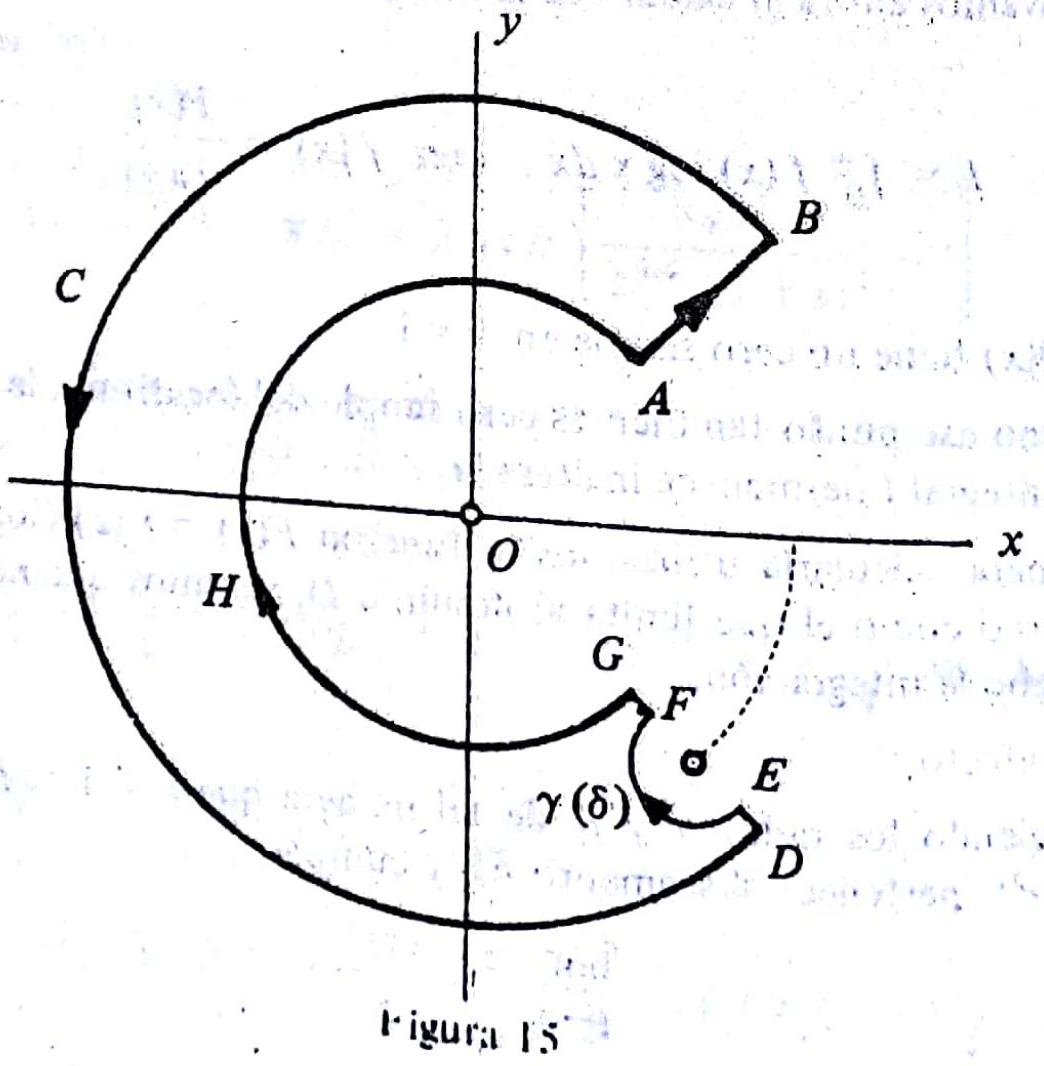
\includegraphics[max width=\textwidth, center]{2025_09_05_adecef5eb2053bc129b5g-113}

Evitamos el punto $z=1$, mediante una semicircunferencia de radio $\delta$.\\
Se aplica el teoremá de los residuos en el dominio así modificado, a la función

$$
F(z)=f(z)(\log z)^{2}
$$

La integral sobre $\overline{\mathrm{AB}}$ tiende, para $\varepsilon \rightarrow 0, r \rightarrow 0$ y $R \rightarrow \infty$, a la integral

$$
I_{2}=\int_{0}^{\infty} f(x)(\log x)^{2} d x
$$

Las integrales sobre $\widehat{B C D}$ y $\widehat{G H A}$ tienden a cero. Respecto de la integral sobre $\overline{\mathrm{DE}}+\gamma(\delta)+\overline{\mathrm{FG}}$, vemos que tiende para $\varepsilon \rightarrow 0, r \rightarrow 0$ y $R \rightarrow \infty$ hacia

$$
\begin{aligned}
& -\int_{0}^{1-\delta} f(\rho)(\log \rho+2 \pi i)^{2} d \rho-\int_{1+\delta}^{\infty} f(\rho)(\log \rho+2 \pi i)^{2} d \rho+ \\
& +\int_{\gamma(\delta)} f(z)(\log z)^{2} d z
\end{aligned}
$$

En un entorno de $z=1$ se tendra:

$$
f(z)(\log z)^{2}=\frac{A}{z-1}+g(z)
$$

con $g(z)$ holomorfa y no nula en $z=1$, pues la determinación que corresponde a arg $1=2 \pi$ tiene un polo simple en $z=1$.

Se llega, entonces, a:

$$
\int_{\gamma(\delta)} \frac{A}{z-1} d z=-\pi A i \quad \text { y } \quad \lim _{\delta \rightarrow 0} \int_{\gamma(\delta)} g(z) d z=0
$$

Como

$$
\begin{aligned}
& A=R[F(z), 1]=\lim _{z \rightarrow 1}(z-1) f(z)(\log z)^{2}= \\
&=(\log 1)^{2} \lim _{z \rightarrow 1}(z-1) f(z)=-4 \pi^{2} R[f(z), 1], \text { es } \\
& \lim _{\delta \rightarrow 0} \int_{\gamma(\delta)} f(z)(\log z)^{2} d z=-i \pi A=4 \pi^{3} i R[f(z), 1] .
\end{aligned}
$$

Como la aplicación del teorema de los residuos al dominio limitado por el contorno indicado y el paso al límite para $\varepsilon \rightarrow 0, r \rightarrow 0, R \rightarrow 0, n_{0 . s}$ da la fórmula


\begin{align*}
& I_{2}-\left[\int_{0}^{1-\delta} f(\rho)(\log \rho)^{2} d \rho+\int_{1+\delta}^{\infty} f(\rho)(\log \rho)^{2} d \rho\right]- \\
& -4 \pi i\left[\int_{0}^{1-\delta} f(\rho)(\log \rho) d \rho+\int_{1+\delta}^{\infty} f(\rho) \log \rho d \rho\right]+ \\
& +4 \pi^{2}\left[\int_{0}^{1-\delta} f(\rho) d \rho+\int_{1+\delta}^{\infty} f(\rho) d \rho\right]+\int_{\gamma(\delta)} f(z)(\log z)^{2} d z= \\
& =2 \pi i \sum R\left[f(z)(\log z)^{2}, z_{k}\right] \tag{27-11}
\end{align*}


pasando al límite para $\delta \rightarrow 0$, el primer miembro se reduce a:

$$
\begin{gathered}
I_{2}-I_{2}-4 \pi i I+4 \pi^{2} \lim _{\delta \rightarrow 0}\left[\int_{0}^{1-\delta} f(\rho) d \rho+\int_{1+\delta}^{\infty} f(\rho) d \rho\right]= \\
=-4 \pi^{3} i R[f(z), 1]+2 \pi i \Sigma R\left[F(z), z_{k}\right],
\end{gathered}
$$

lo que se puede escribir como:

$$
\begin{aligned}
& I+i \pi \lim _{\delta \rightarrow 0}\left[\int_{0}^{1-\delta} f(\rho) d \rho+j_{1+\delta}^{\infty} f(\rho) d \rho\right]= \\
& =\pi^{2} R\left[f(z), 1 \Gamma-\frac{1}{2} \Sigma R\left[F(z)(\log z)^{2}, z_{k}\right]\right.
\end{aligned}
$$

e igualando las partes reales se obtiene la fórmula

$$
I=R e\left\{\pi^{2} R\left[f^{\prime}(z), 1\right]-\frac{1}{2} \sum R\left[F(z)(\log z)^{2}, z_{k}\right]\right\}
$$

Observemos que como $f(x)$ no es integrable en $(0, \infty)$ (por tener un polo en $x=1$ ) el

$$
\lim _{\delta \rightarrow 0}\left[\int_{0}^{1-\delta} f(\rho) d \rho+\int_{1+\delta}^{\infty} f(\rho) d \rho\right]
$$

no es la

$$
\int_{0}^{\infty} f(\rho) d \rho
$$

sino su valor principal, que existe al existir lọs límites de los otros términos en el primer miembro de (27-11).

\section*{Ejemplo}
Calculemos

$$
I=\int_{0}^{\infty} \frac{\log x}{x^{2}-1} d x
$$

Se tiene

$$
\begin{gathered}
R\left[\frac{(\log z)^{2}}{z^{2}-1},-1\right]=\frac{[\log (-1)]^{2}}{(-2)}=\frac{-(i \pi)^{2}}{2}=\frac{\pi^{2}}{2} \\
R\left[\frac{1}{z^{2}-1}, 1\right]=\frac{1}{2}
\end{gathered}
$$

De acuerdo con lo anterior

$$
\int_{0}^{\infty} \frac{\log x}{x^{2}-1} d x=\frac{\pi^{2}}{2}-\frac{\pi^{2}}{4}=\frac{\pi^{2}}{4}
$$

Cuando la función es par o impar, se puede usar el segundo contorno, evitando el punto $z=-1$ (en el que la función tiene un polo de primer orden), con una semicircunferencia. Los cálculos son análogos a los anteriores, aunque más simples.

\section*{Ejercicios}
\begin{enumerate}
  \item Resolver la ecuación de segundo grado
\end{enumerate}

$$
z^{2}-(2 i+4) z+10 i-5=0
$$

Respuesta: 5 y $-1+2 i$.\\
2. Demostrar que si $a+b i$ es solución de la ecuación

$$
a_{0} \mathrm{z}^{n}+a_{1} z^{n-1}+\cdots+a_{n}=0
$$

de coeficientes reales, entonces $a-b i$ es también solución de la misma ecuación.\\
3. Resolver la ecuación

$$
|z|-z=1+2 i
$$

Respuesta: $3 / 2-2 i$.\\
4. Determinar la homografía que hace corresponder a los puntos $1, i,-1$ los puntos $2,0,1$ respectivamente.\\
5. Sea $t$ un número real y $a$ un número complejo de módulo menor que 1 . Demostrar que la función

$$
f(z)=(\cos t+i \operatorname{sen} t) \frac{z-a}{1-\bar{a} z}
$$

transforma la circunferencia $|z|=1$ en sí misma.\\
6. Dada la homografía

$$
f(z)=\frac{z-i}{z+i}
$$

determinar en qué se transforma la región definida por las dos condiciones $x>0,|z|<1$ siendo $z=x+i y$.\\
7. Sea $a$ un número real mayor que cero y sea $D$ el dominio del plano situado en el primer cuadrante y limitado además por las hipérbolas de ecuaciones: $x . y=a ; x . y=2 a$.\\
a) Determinar la imagen de $D$ por la aplicación $f(z)=z^{2}$.\\
b) Determinar la imagen por la aplicación anterior de la semibanda: $0<x<k$; $0<y$.\\
8. Sean $f$ y $g$ las funciones siguientes (para $z=x+i y$ ):

$$
\begin{gathered}
f(z)=+\sqrt{|x \cdot y|} \\
g(z)=\frac{x^{3}-y^{3}+i\left(x^{3}+y^{3}\right)}{x^{2}+y^{2}}
\end{gathered}
$$

para $z$ distinto de cero y $g(0)=0$.\\
Demostrar que en el punto $z=0$, ambas funciones son continuas, cumplen las condiciones de Cauchy-Riemann y no son monógenas.\\
9. Se da la siguiente función (para $z=x+i y$ ):

$$
f(z)=\frac{x^{3} y+i x^{2} y^{2}}{x^{4}+y^{2}},
$$

para $z$ distinto de cero y $f(0)=0$. Probar que en $z=0$ se tienen las siguientes propiedades:\\
a) Condiciones de Cauchy-Riemann.\\
b) Hay derivadas a lo largo de cualquier recta y todas esas derivadas son iguales.\\
c) La función no es monógena.\\
10. Determinar los puntos de monogeneidad y de holomorfismo de las siguientes funciones (para $z=x+i y$ ):\\
a) $f(z)=\frac{x-i y}{x^{2}+y^{2}} \quad$ para $z \neq 0, f(0)=0$;\\
b) $g(z)=x-i y$;


c) $h(z)=x^{2}+i y^{2}$\\
d) $k(z)=x^{2}-y^{2}-2 x y+i\left(x^{2}-y^{2}+2 x y\right)$.

\section*{Respuestas:}
$f$ es holomorfa para $z \neq 0 ; g$ no es monógena en ningún punto; $h$ es monógena en los puntos de la recta $x=y$ y no es holomorfa en ningún punto; $k$ es holomorfa en todo punto. Obsérvese además que $f(z)=1 / z$ y $k(z)=z^{2}(1+i)$.\\
11. Demostrar que las funciones $e^{x} \cos y$ y $\cos x$ sh $y$ son armónicas en todo el plano. Determinar la función holomorfa $f$ cuya parte real es $e^{x} \cos y$ y la función holomorfa $g$ cuya parte imaginaria es $\cos x$ sh $y$.

\section*{Respuestas:}
$f(z)=e^{x} \cos y+i e^{x} \operatorname{sen} y+i C: C$ es un número real arbitrario, $y$\\
$g(z)=\operatorname{sen} x \operatorname{ch} y+C+i \cos x$ sh $y ; C$ es un número real arbitrario.\\
12. Determinar la función $f(z)=u(x, y)+v(x, y) i$, sabiendo que es holomorfa en todo el plano y que $u(x, y)+v(x, y)=x^{2}-y^{2}+2 x y$.\\
Respuesta: $z^{2}+C(1-i)$, para $C$ real cualquiera.\\
13. Determinar la función $f$ holomorfa en todo el plano cuya parte real es $e^{x}(x \cos y-y \operatorname{sen} y)$.

\section*{Respuesta:}
$(x+i y) e^{x}(\cos y+i \operatorname{sen} y)+i C ; C$ real arbitrario.\\
14. Dada la función

$$
u(x, y)=\frac{\operatorname{sen} 2 x}{\operatorname{ch} 2 y-\cos 2 x}
$$

determinar la función holomorfa que tiene $u(x, y)$ como parte real.\\
15. Dada la función

$$
f(z)=\frac{z-1}{z+1}
$$

determinar las imágenes por $f$ de las curvas $|z|=c$ y arg $z=k$, siendo $k$ y c constantes arbitrarias.

\section*{Respuesta:}
Circunferencias de centros en los dos ejes.\\
16. Sea $D$ el dominio del plano complejo de finido por las desigualda. des

$$
r<|z|<R \quad ; \quad t<\arg z<T \text {, }
$$

y sea, pará $n$ entero arbitrario $f(z)=\left(z^{n}+z^{-n}\right) ; 2$. cónicas.

Demostrar que el dominio transformado de $D$ por $f$ está limitado por\\
17. Calcular

$$
\int_{S} z^{2} d z,
$$

en donde $S$ es el segmento ( $2+3 i ; 4+6 i$ ) sin utilizar la fórmula de Barrow y comprobar el resultado aplicando dicha fórmula.\\
18. Calcular las integrales (para $z=x+i y$ )\\
a) $\int_{s}\left(x^{2}+i y^{3}\right) d z \quad s$ es el segmento $(1, i)$;\\
b) $\int_{0}^{1+i}(z+1) d z \quad$ y\\
c) $\int_{L} x d z ; L$ es la circunferencia $|z|=1$ en sentido positivo.

Respuestas:\\
а) $\frac{-7+i}{12}$;\\
b) $1+2 i$;\\
c) $\pi i$.\\
19. Calcular la integral de $|z|$ entre los puntos $i$ y - $i$ recorriendo los caminos siguientes:\\
a) El segmento rectilíneo que une $-i$ con $i$.


b) La semicircunferencia unitaria que une ambos puntos en unou otro sentido.\\
20. Sin utilizar otros recursos que los contenidos en los seis primeros parágrafos del texto calcular las integrales\\
а) $\int_{l} \frac{z^{2}+4}{z} d z \quad$;\\
b) $\int_{I \cdot} \cdot\left(\frac{1}{z+1}+\frac{2}{z-3}\right) d z$;\\
c) $\int_{l . "} \frac{d z}{z^{2}-1}$\\
d) $\int_{\text {L }}$ "' $\frac{d z}{z^{4}+5 z^{2}+4}$,\\
donde $L, L$ ', $L$ '' y $L$ ''' son las circunferencias de centro en el origen reco. rridas en sentido positivo y cuyos radios son respectivamente $1,4,2$ y $3 / 2$. Respuestas:\\
а) $8 \pi i \quad$;\\
b) $6 \pi i$;\\
c) 0 ;\\
d) 0 .\\
21. Sea $f$ una función holomorfa en $|z|<R$ con $R>1$. Demostrarlas fórmulas:

$$
\begin{gathered}
2 f(0)+f^{\prime}(0)=\frac{2}{\pi} \int_{0}^{2 \pi} f\left(e^{i \varphi}\right) \cos ^{2} \frac{\varphi}{2} d \varphi \\
f^{\prime}(0)=\frac{1}{\pi} \int_{0}^{2 \pi} f\left(e^{i \varphi}\right) \cos \varphi d \varphi
\end{gathered}
$$

Indicación: calcular de dos formas distintas la integral

$$
\int_{|z|=1}\left(2+z+\frac{1}{z}\right) f(z) \frac{d z}{z}
$$

\begin{enumerate}
  \setcounter{enumi}{21}
  \item Determinar los puntos de holomorfismo de las funciones siguientes (para $z=x+i y$ ):\\
a) $f^{\prime}(z)=x^{2}+y^{2}+2 x y i$;\\
b) $g(z)=2 x-3 y+i(3 x+2 y)$;\\
c) $h(z)=\frac{x+i y}{x^{2}+y^{2}}$ y\\
d) $k(z)=\left|x^{2}-y^{2}\right|+2 i|x y|$.
\end{enumerate}

\section*{Respuestas:}
a) monógena en la recta $y=0$; holomorfa en ningún punto.\\
b) holomorfa en todo punto.\\
c) no es monógena en ningún punto,\\
d) holomorfa en los cuatro abiertos siguientes:\\
$0<\arg z<\frac{\pi}{4} ; \frac{\pi}{2}<\arg z<\frac{3 \pi}{4} ; \pi<\arg z<\frac{5 \pi}{4} ; \frac{3 \pi}{2}<\arg z<\frac{7 \pi}{4}$\\
23. Calcular la integral de la función $\operatorname{Re}(z)$, es decir parte real de $z$, a lo largo de los dos caminos siguientes:\\
a) La recta que une los dos puntos ( 0 y $1+i$ );\\
b) La poligonal de vértices $0,1,1+i$.

Respuesta:\\
a) $\frac{1+i}{2}$\\
b) $\frac{1}{2}+i$.\\
24. Calcular la integral

$$
\int_{E} z^{-1} d z \quad \text { siendo } E \text { la elipse de ecuación }
$$

$$
\frac{x^{2}}{a^{2}}+\frac{y^{2}}{b^{2}}=1
$$

$e^{-b z^{2}}{ }^{25}$. Mediante la aplicación del teorema de Cauchy a la función en el rectángulo de vértices

$$
R,-R,-R-\frac{i a}{2 b}, R-\frac{i a}{2 b}
$$

(con $a, b$ reales y mayores que cero), calcular la integral

$$
\int_{-\infty}^{\infty} e^{i a x-b x^{2}} d x
$$

Observación: para este ejercicio y los dos siguientes se supone conocida la fórmula

$$
\int_{-\infty}^{\infty} e^{-u^{2}} d u=\sqrt{\pi}
$$

\begin{enumerate}
  \setcounter{enumi}{25}
  \item Mediante la aplicación del teorema de Cauchy a la función $e^{-a z^{2}}$ (a real y mayor que cero) en el rectángulo de vértices $R, R$, $R+i b,-R+i b$, con $b$ mayor que cero, calcular el valor de la integral real:
\end{enumerate}

$$
\int_{-\infty}^{\infty} e^{-a x^{2}} \cos (2 a b x) d x
$$

Respuesta:

$$
\sqrt{\frac{\pi}{a}} e^{-a b^{2}}
$$

\begin{enumerate}
  \setcounter{enumi}{26}
  \item Calcular la integral (para $a$ real y mayor que cero):
\end{enumerate}

$$
\int_{0}^{\infty} e^{-x} \frac{\operatorname{sen}(a x)}{\operatorname{sh}(x)} d x
$$

mediante la aplicación del teorema de Cauchy en el dominio $D$ definido de la manera siguiente: se toman los seis puntos, $r, R, R+i, r+i,(1-r) i, r i$; la frontera de $D$ se obtiene uniendo estos puntos en la forma siguiente: el primero y el segundo, el segundo y el tercero, el tercero y el cuarto, el quinto y el sexto con segmentos de recta, en cambio el cuarto y quinto y el sexto y primero se unen con cuadrantes de circunferencia.

\section*{Respuesta:}
$$
\left(e^{a}+1\right)\left(1-e^{a}\right)^{-1 / 2}-a^{-1} .
$$

\begin{enumerate}
  \setcounter{enumi}{27}
  \item Calcular las denominadas integrales de Fresnel
\end{enumerate}

$$
\int_{0}^{\infty} \cos \left(x^{2}\right) d x \quad ; \quad \int_{0}^{\infty} \operatorname{sen}\left(x^{2}\right) d x,
$$

mediante la aplicación del teorema de Cauchy a la función $e^{i z^{2}}$ en el sector circular de centro $z=0$ y vértices $R$ y $R e^{i \pi / 4}$.\\
Respuesta:\\
Ambas integrales valen $\frac{\sqrt{2 \pi}}{4}$.\\
29. Calcular los radios de convergencia de las siguientes series de potencias:\\
a) $\sum_{1}^{\infty} \frac{(1+2 i)^{n} n!}{n^{n}} z^{n} \quad$;\\
b) $\sum_{1}^{\infty} \frac{z^{n}}{1+(1+i)^{n}}$\\
c) $\sum_{1}^{\infty} \frac{z^{n}}{n^{n}} \quad$;\\
d) $2^{-1} z+3^{-2} z^{2}+2^{-3} z^{3}+3^{-4} z^{4}+\cdots$;\\
е) $\sum_{0}^{\infty} \frac{z^{n^{2}}}{2^{n}} \quad$;\\
f) $\sum_{0}^{\infty} n!z^{n^{2}} \quad y$\\
g) $\sum_{0}^{\infty} \frac{n!}{(2-i) n^{2}} z^{n}$.

Estudiar el comportamiento en el borde del disco de convergencia.\\
Respuestas:\\
a) $R=e \sqrt{5}$, no converge en ningún punto del borde;\\
b) $R=\sqrt{2}$, no converge en ningún punto del borde;\\
c) $R=\infty$;\\
d) $R=2$, no converge en ningún punto del borde;\\
e) $R=1$, converge en todos los puntos del borde;\\
f) $R=1$, no converge en ningún punto del borde;\\
g) $R=\infty$.\\
30. La serie de potencias de término general $a_{n} z^{n}$, tiene un radio de convergencia $R$ que no es ni cero ni infinito. Determinar el radio. de convergencia de las series de término general:\\
a) $n^{p} a_{n} z^{n} \quad$;\\
b) $\frac{1}{n!} a_{n} z^{n}$\\
y\\
c) $n a_{n}^{p} z^{n}$,

Siendo $p$ un entero positivo.

\section*{Respuestas:}
a) $R$\\
b) $\infty$;\\
c) $R^{p}$.\\
31. Dar un ejemplo de dos series de potencias que tengan el mismo radio finito de convergencia y tales que la serie suma tenga $\infty$ como radio de convergencia. ¿Qué se puede decir en el caso en que las dos series tengan distintos radios de convergencia?\\
32. Dados los dominios planos:\\
a) $0<y<\pi$;\\
b) $0<y<\pi, x<0$;\\
c) $0<y<\pi, 0<a<x<b$ determinar sus imágenes mediante la función $e^{z}$.\\
33. Dados los dominios planos:\\
а) $-\pi / 2<x<\pi / 2, y>0$;\\
b) $0<x<\pi / 2, y>0$;\\
c) $x<\pi / 2,0<y<k$,\\
determinar sus imágenes mediante la función sen $z$.\\
34. Demostrar la fórmula, para $z$ complejo arbitrario:

$$
\lim _{n \rightarrow \infty}\left(1+\frac{z}{n}\right)^{n}=e^{z}
$$

\begin{enumerate}
  \setcounter{enumi}{33}
  \item Dada la función $f(z)=e^{-z^{-4}}$ para $z \neq 0$ y $f(0)=0$; demostrar que cumple las condiciones de Cauchy-Riemann en $z=0$, pero es discontinua en dicho punto.
  \item Sea $D$ un conjunto acotado abierto y conexo del plano complejo; sea $D^{\prime}$ otro abierto y conexo y sea $C$ la frontera de $D^{\prime}$. Se supone que $C \cup D^{\prime} \subset D$.
\end{enumerate}

Sea $f$ una función holomorfa y no constante en $D$ y tal que $|f(z)|$ es constante sobre $C$. Demostrar que $f$ tiene al menos una raíz en $D^{\prime}$.\\
36. Deducir directamente del principio del máximo otra demostración del teorema de D'Alembert.\\
37. Desarrollar en serie de potencias de $(z-1)$ la función

$$
f(z)=\frac{1}{z-2}
$$

por los siguientes métodos:\\
a) por división;\\
b) por el cálculo de las derivadas;\\
c) como suma de una serie geométrica.\\
38. Desarrollar en serie de potencias de $(z+1-i)$ la función $z^{-1}$.

Respuesta:

$$
z^{-1}=-\sum_{0}^{\infty} \frac{(1+i)^{n+1}}{2^{n+1}}(z+1-i)^{n}
$$

\begin{enumerate}
  \setcounter{enumi}{38}
  \item Desarrollar en serie de Laurent la función
\end{enumerate}

$$
f(z)=\frac{2}{z^{3}-3 z^{2}+2 z}
$$

en la corona $1<|z|<2$.

Respuesta:

$$
f(z)=-\sum_{-2}^{\infty} \frac{2}{z^{n}}-\frac{1}{z}+\sum_{0}^{\infty} \frac{-1}{2^{n+1}} z^{n}
$$

\begin{enumerate}
  \setcounter{enumi}{39}
  \item Calcular el desarrollo en serie de Laurent de la función $F(z)=e^{z}(z-1)^{-1}$ en el dominio $|z|>1$.
\end{enumerate}

Respuesta:

$$
F(z)=\sum_{1}^{\infty} \frac{e}{z^{n}}+\sum_{0}^{\infty}\left(e-\sum_{0}^{n} \frac{1}{k!}\right) z^{n}
$$

\begin{enumerate}
  \setcounter{enumi}{40}
  \item Calcular el desarrollo en serie de Laurent de la función
\end{enumerate}

$$
f(z)=\frac{1}{z(z-1)^{2}}
$$

\section*{Respuestas:}
а) $R \quad$;\\
b) $\infty$;\\
c) $R^{p}$.\\
31. Dar un ejemplo de dos series de potencias que tengan el mismo radio finito de convergencia y tales que la serie suma tenga $\infty$ como radio de convergencia. ¿Qué se puede decir en el caso en que las dos series tengan distintos radios de convergencia?\\
32. Dados los dominios planos:\\
a) $0<y<\pi$;\\
b) $0<y<\pi, x<0$;\\
c) $0<y<\pi, 0<a<x<b$ determinar sus imágenes mediante la función $e^{z}$.\\
33. Dados los dominios planos:\\
a) $-\pi / 2<x<\pi / 2, y>0$;\\
b) $0<x<\pi / 2, y>0$;\\
c) $x<\pi / 2,0<y<k$, determinar sus imágenes mediante la función sen $z$.\\
34. Demostrar la fórmula, para $z$ complejo arbitrario:

$$
\lim _{n \rightarrow \infty}\left(1+\frac{z}{n}\right)^{n}=e^{z}
$$

\begin{enumerate}
  \setcounter{enumi}{33}
  \item Dada la función $f(z)=e^{-z^{-4}}$ para $z \neq 0$ y $f(0)=0$; demostrar que cumple las condiciones de Cauchy-Riemann en $z=0$, pero es discontinua en dicho punto.
  \item Sea $D$ un conjunto acotado abierto y conexo del plano complejo; sea $D^{\prime}$ otro abierto y conexo y sea $C$ la frontera de $D^{\prime}$. Se supone que $C \cup D^{\prime} \subset D$.
\end{enumerate}

Sea $f$ una función holomorfa y no constante en $D$ y tal que $|f(z)|$ es constante subre $C$. Demostrar que $f$ tiene al menos una raíz en $D^{\prime}$.\\
36. Deducir directamente del principio del máximo otra demostración del teorema de D'Alembert.\\
37. Desarrollar en serie de potencias de $(z-1)$ la función

$$
f(z)=\frac{1}{z-2}
$$

por los siguientes métodos:\\
a) por división;\\
b) por el cálculo de las derivadas;\\
c) como suma de una serie geométrica.\\
38. Desarrollar en serie de potencias de $(z+1-i)$ la función $z^{-1}$.

Respuesta:

$$
z^{-1}=-\sum_{0}^{\infty} \frac{(1+i)^{n+1}}{2^{n+1}}(z+1-i)^{n}
$$

\begin{enumerate}
  \setcounter{enumi}{38}
  \item Desarrollar en serie de Laurent la función
\end{enumerate}

$$
f(z)=\frac{2}{z^{3}-3 z^{2}+2 z}
$$

en la corona $1<|z|<2$.\\
Respuesta:

$$
f(z)=-\sum_{-2}^{\infty} \frac{2}{z^{n}}-\frac{1}{z}+\sum_{0}^{\infty} \frac{-1}{2^{n+1}} z^{n}
$$

\begin{enumerate}
  \setcounter{enumi}{39}
  \item Calcular el desarrollo en serie de Laurent de la función $F(z)=e^{z}(z-1)^{-1}$ en el dominio $|z|>1$.
\end{enumerate}

Respuesta:

$$
F(z)=\sum_{1}^{\infty} \frac{e}{z^{n}}+\sum_{0}^{\infty}\left(e-\sum_{0}^{n} \frac{1}{k!}\right) z^{n}
$$

\begin{enumerate}
  \setcounter{enumi}{40}
  \item Calcular el desarrollo en serie de Laurent de la función
\end{enumerate}

$$
f(z)=\frac{1}{z(z-1)^{2}}
$$

en los dominios: a) $0<|z-1|<1 ;$ b) $|z-1|>1$.\\
Respuestas:\\
а) $\sum_{0}^{\infty}(-1)^{n}(z-1)^{n-2}$;\\
b) $\sum_{0}^{\infty}(-1)^{n}(z-1)^{-(n+3)}$.\\
42. Sean $f$ una función que tiene un polo simple en el origen $y x$ un complejo arbitrario. Sea $g$ la función

$$
g(z)=\frac{f^{\prime}(z)}{f(z)-x}
$$

Demostrar que el desarrollo en serie de Laurent de $g$ en el entorno de 0 es de la forma

$$
-\frac{1}{z}+p_{1}(x) z+\cdots+p_{n+1}(x) z^{n}+\cdots
$$

siendo $p_{k}$ un polinomio en $x$ de grado $k$.\\
43. Determinar los desarrollos en serie de Laurent de la función

$$
f(z)=\frac{1}{z^{2}-3 z+2}
$$

en los dominios siguientes:\\
а) $|z|<1 \quad$;\\
b) $1<|z|<2$\\
y\\
c) $|z|>2$.

Respuestas:\\
a) $f(z)=\sum_{0}^{\infty}\left(1-\frac{1}{2^{n+1}}\right) z^{n}$;\\
b) $f(z)=-\sum_{1}^{\infty} z^{-n}-\sum_{0}^{\infty} \frac{1}{2^{n+1}} z^{n} \quad$ y\\
c) $f(z)=\sum_{1}^{\infty}\left(2^{n-1}-1\right) z^{-n}$.\\
44. Demostrar que en $0<|z|<\pi$ la función

$$
f(z)=\frac{1}{z^{2} \operatorname{sh} z}
$$

tiene un desarrollo en serie de Laurent de la forma

$$
A z^{-3}+B z^{-2}+C z+a_{0}+a_{1} z+\cdots+a_{n} z^{n}+\cdots
$$

y calcular $A, B, C, a_{0}$ y $a_{1}$.\\
Respuesta:

$$
A=1 ; B=0 ; C=-\frac{1}{6} ; a_{0}=0 ; a_{1}=\frac{7}{360} .
$$

\begin{enumerate}
  \setcounter{enumi}{44}
  \item Determinar y clasificar todos los puntos singulares en el plano complejo compactificado de las siguientes funciones:\\
$\frac{1}{z^{3}-7 z^{2}+z+5}+z e^{z^{-1}} \quad ; \frac{z^{5}}{1+z^{4}} ;\left[\operatorname{sen}\left(z^{-2}\right)\right]^{-1} ;$
\end{enumerate}

$$
e^{z(1 \cdot z)^{-1}} \quad ; \frac{\cos z-\operatorname{sen} z}{z^{4}+2 z^{2}+1} \quad ; \quad \operatorname{sen}\left(z^{-1}\right)+z^{-2} \quad \text { y } \operatorname{sen}\left[\cos \left(z^{-1}\right)^{-1}\right] .
$$

\begin{enumerate}
  \setcounter{enumi}{45}
  \item Demostrar que la función
\end{enumerate}

$$
\frac{1}{\operatorname{sen} z}+\frac{z^{2}+\pi^{2}}{z^{3}-\pi^{2} z}
$$

es holomorfa en el disco $|z|<2$.\\
Deducir de este resultado que $1 / \operatorname{sen} z$ admite en la corona $\pi<|z|<2 \pi$ un desarrollo en serie de Laurent de la forma:

$$
-2 \sum_{1}^{\infty} \frac{\pi^{2 n}}{z^{2 n+1}}-\frac{1}{z}+\sum_{0}^{\infty} a_{n} z^{n}
$$

\begin{enumerate}
  \setcounter{enumi}{46}
  \item Se consideran las funciones
\end{enumerate}

$$
f(z)=\frac{2}{\operatorname{sen}^{2} z} \quad \text { y } \quad g(z)=\sum_{-\infty}^{\infty} \frac{1}{(z-n)^{2}} .
$$

Estudiar sus puntos singulares y sus propiedades de periodicidad.\\
Demostrar que la función $h(z)-f(z)$ es una función entera.\\
Sea $z=x+i y$. Demostrar que, en la banda $0 \leqslant|x| \leqslant 1, f$ y $g$ tienden a cero cuando $|y|$ tiende a infinito.

Deducir para $z$ no entero la tórmula

$$
\operatorname{sen}^{2}(\pi z)^{-1}=\pi^{-2} \Sigma(z-n)^{-2} .
$$

\begin{enumerate}
  \setcounter{enumi}{47}
  \item Calcular los siguientes residuos:\\
a) de $z^{-2}(z-1)^{-1}$ en $z=0$ :
\end{enumerate}

Respuesta: -1.\\
b) de $z^{-2}\left(z^{2}-1\right)^{-1}$ en $z=0$.

Respuesta: 0.\\
c) de $z e^{z}\left(z^{2}-1\right)^{-1}$ en $z=1$.

Respuesta: e/2.\\
d) de $e^{z}(z-1)^{-2} z^{-1}$ en $z=0$ y $z=1$.

Respuestas: 1 y 0 .\\
e) de $z^{3}(z-1)^{-1}(z-2)^{-1}(z-3)^{-1}$ en el punto del infinito.

Respuesta: - 6.\\
f) de $e^{a z}\left(1+e^{z}\right)^{-1}$ en $z=\pi i$.

Respuesta: $-e^{-a \pi i}$

156\\
g) de $\operatorname{cotg} z$ en $z=n \pi$.

Respuesta: 1.\\
49. Dada la función $f(z)=e^{1 / z}(z+1)^{-1} z^{-1}$ clasificar sus puntos singulares, calcular directamente los residuos en cada uno de esos puntos y comprobar que la suma es cero.\\
50. Probar que si

$$
f(z)=A_{1}(z-a)^{-1}+A_{2}(z-a)^{-2}+\cdots+A_{n}(z-a)^{-n}
$$

el residuo de $f(z)(z-b)^{-1}$ es $-f(b)$.\\
51. Demostrar que la función $f(z)=z^{-1}\left(e^{z}-1\right)^{-1}$ admite en el entorno de cero un desarrollo en serie de Laurent de la forma:

$$
z^{-2}-(2 z)^{-1}+a_{0}+a_{2} z^{2}+\cdots+a_{2 n} z^{2 n}+\cdots
$$

y determinar los valores de $a_{0}$ y $a_{2}$.\\
Respuestas:

$$
\frac{1}{12} \text { y }-\frac{1}{720} \cdots
$$

\begin{enumerate}
  \setcounter{enumi}{51}
  \item Se considera la función
\end{enumerate}

$$
f(z)=\frac{i-4 e^{(1-z)^{-1}}}{i-e^{(1-z)^{-1}}}
$$

Demostrar que $f$ es meromorfa en el complementario, respecto del plano complejo, del punto $z=1$. ¿Cuál es el orden de sus polos? Demostrar que en todo entorno del punto $z=1$, la función $g(z)=f(z)-w$ tiene una raíz, cualquiera que sea el valor de $w$ con excepción de los valores $w=1$ y $w=4$.\\
53. Sèa $f$ una función que tiene un polo simple en $z=-1$ y un polo doble en $z=2$, en los demás puntos (incluyendo el del infinito) $f$ es holomorfa. Los residuos de $f$ en -1 y 2 son respectivamente 1 y 2 . Además se conocen los valores de $f$ en 0 y $1: f(0)=7 / 4, f(1)=5 / 2$.

Se pide: determinar $f$ y calcular su desarrollo en serie de Laurent de potencias de $z$ en la corona $1<|z|<2$.

\section*{Respuesta}
$$
f(z)=\frac{z^{3}-3 z+7}{(z+1)(z-2)^{2}} \quad ; f(z)=\frac{3}{4}+\sum_{1}^{\infty} \frac{n-3}{2^{n+2}} z^{n}+\sum_{1}^{\infty} \frac{(-1)^{n+1}}{z^{n}}
$$

\begin{enumerate}
  \setcounter{enumi}{53}
  \item Sea $C$ la circunferencia $|z|=2$ recorrida en sentido positivo. Calcular:\\
а) $\int_{C} \frac{z}{z^{4}-1} d z$;\\
b) $\int_{C} \frac{1+\operatorname{sen} z}{\operatorname{sen}^{2} z} d z \quad y$\\
c) $\int_{C} \frac{d z}{(z+1)^{4}\left(z^{2}-9\right)(z-4)}$.
\end{enumerate}

Respuestas:\\
a) 0 ;\\
b) $2 \pi i \quad$;\\
c) $\frac{341 \pi i}{160.000}$.\\
55. Calcular

$$
\int_{0}^{2 \pi} \frac{d t}{5+4 \cos t}
$$

Respuesta: $2 \pi / 3$.\\
56. Calcular

$$
\int_{-\pi}^{\pi} \frac{d t}{a+b \cos t},
$$

siendo $a$ y $b$ reales y $a>|b|$. ¿Por qué es necesario imponer esta última condición?

\section*{Respuesta:}
$2 \pi\left(a^{2}-b^{2}\right)^{-1 / 2}$.\\
57. Determinar, mediante la aplicación de la fórmula de Schwarz, la función holomorfa $f$ cuya parte real sobre la circunferencia $|z|=1$ es

$$
\frac{2 \cos \varphi-1}{5-4 \cos \varphi}
$$

Respuesta:\\
$z(2-z)^{-1}+C i$.\\
58. Calcular la integral

$$
I(R)=\int_{C(R)} \frac{d z}{z^{6}(z-2)(z-3)}
$$

\begin{enumerate}
  \setcounter{enumi}{58}
  \item Calcular la integral $(a>b>0)$
\end{enumerate}

$$
\int_{0}^{2 \pi} \frac{d \varphi}{(a+b \cos \varphi)^{2}}
$$

Respuesta:\\
$2 \pi a\left(a^{2}-b^{2}\right)^{-3 / 2}$.\\
60. Calcular las integrales

$$
\int_{-\infty}^{\infty} \frac{x^{2}}{1+x^{4}} d x \quad y \quad \int_{-\infty}^{\infty} \frac{x^{2}}{x^{4}+5 x^{2}+1} d x .
$$

Respuestas:

$$
\pi \frac{\sqrt{2}}{2} \quad ; \pi / 6
$$

\begin{enumerate}
  \setcounter{enumi}{60}
  \item Calcular el valor principal de la integral
\end{enumerate}

$$
\int_{-\infty}^{\infty} \frac{d x}{x^{3}-4 x^{2}+5 x}
$$


\section*{Respuesta:}
$2 \pi / 5$.\\
62. Calcular para $n$ y $m$ enteros positivos con $p<n$ el valur de la integral

$$
\int_{0}^{\infty} \frac{x^{2 p}}{1+x^{2 n}} d x
$$

\section*{Respuesta:}
$$
\frac{\pi}{2 n \operatorname{sen}\left[\pi(2 p+1)^{\prime 2} n\right]}
$$

\begin{enumerate}
  \setcounter{enumi}{62}
  \item Demostrar la fórmula
\end{enumerate}

$$
\int_{-\infty}^{\infty} \frac{d x}{\left(1+x^{2}\right) \operatorname{ch} x}=\frac{\pi}{\cos 1}+8 \pi \sum_{1}^{\infty} \frac{(-1)^{n}}{(2 n-1)^{2} \pi^{2}-4}
$$

\begin{enumerate}
  \setcounter{enumi}{63}
  \item Calcuiar, para a y mi ruales y mayores que cero, el valor de la integral
\end{enumerate}

$$
\int_{-\infty}^{\infty} \frac{\cos m x+\operatorname{sen} m x}{a^{2}+x^{2}} d x
$$

\section*{Respuesta:}
$\pi e^{-m a} a^{-1}$.\\
65. Sean $p$ y $n$ dos enteros positivos. Consideremos las dos integrales:


\begin{align*}
& I_{1}=\int_{0}^{2 \pi} e^{p} \cos t \operatorname{sen}(n t-p \operatorname{sen} t) d t  \tag{y}\\
& \quad I_{2}=\int_{0}^{2 \pi} e^{p \cos t} \cos (n t-p \operatorname{sen} t) d t
\end{align*}


Determinar una funciun $j$ (こ) iai quic

$$
I_{1}+I_{2} i=\int_{1}, f(z) d z,
$$

en donde $\Gamma$ es la circunferencia $|z|=1$ recorrida en sentido positivo. Calcular $I_{1}$ e $I_{2}$.

Respuestas:

$$
I_{1}=0 \quad \text { e } \quad I_{2}=\frac{2 \pi p^{n}}{n!} .
$$

\begin{enumerate}
  \setcounter{enumi}{65}
  \item Calcular las integrales
\end{enumerate}

$$
\int_{-\infty}^{\infty} \frac{\left(x^{2}-1\right) \operatorname{sen} x}{x^{3}+x} d x \quad y \quad \int_{-\infty}^{\infty} \frac{\operatorname{sen} x}{x\left(x^{2}+1\right)^{2}} d x
$$

Respuestas:

$$
\frac{2 \pi}{e}-\pi \quad ; \quad \pi\left(1-\frac{3}{2 e}\right)
$$

\begin{enumerate}
  \setcounter{enumi}{66}
  \item Calcular la integral
\end{enumerate}

$$
\int_{-\infty}^{\infty} \frac{\cos x}{\pi^{2}-4 x^{2}} d x
$$

Respuesta:\\
1/2\\
68. Calcular la integral

$$
\int_{0}^{\infty}\left(\frac{\operatorname{sen} x}{x}\right)^{2} d x .
$$

Indicación: considerar la función

$$
\frac{1-e^{2 i z}}{z^{2}},
$$

y aplicar el teorema de los residuos sobre un dominio apropiado.

\section*{Respuesta:}
1/2\\
69. Calcular la integral

$$
\int_{-\infty}^{\infty} \frac{e^{2 \pi x / 3}}{\operatorname{ch} \pi x} d x
$$

utilizando como dominio para la aplicación del teorema de los residuos el rectángulo de vértices $-a ; a ; a+i ;-a+i$.\\
Respuesta: $\frac{\pi}{2}$\\
70. Calcular por el método de los residuos la integral

$$
\int_{-\infty}^{\infty} \frac{e^{4 x}}{1+e^{6 x}} d x
$$

Comprobar el xesultado haciendo el cambio de variable $e^{2 x}=t y$ calculando de nuevo la integral resultante por el método de los residuos.\\
71. Sea $f$ una función meromorfa en $|z| \leqslant R$ sin polos ni ceros en $|z|=R$. Sea $g$ una función holomorfa y no nula en $|z| \leqslant R$.\\
fórmula\\
Sea $a_{1}, \ldots, a_{m}$ los ceros de $f$ y $b_{1}, \ldots, b_{n}$ sus polos. Demostrar la

$$
\frac{1_{1}}{2 \pi i} \int_{\Gamma} \frac{f^{\prime}(z)}{f(z)} g(z) d z=\sum_{1}^{m} p_{j} g\left(a_{j}\right)-\sum_{1}^{n} q_{k} g\left(b_{k}\right),
$$

en donde $\Gamma$ es la circunferencia $|z|=R$ recorrida en sentido positivo, $p_{j}$ es el orden del cero $a_{j}$ y $q_{k}$ es el orden del polo $b_{k}$.\\
72. Demostrar la fórmula

$$
\int_{0}^{\infty} \frac{x^{a-1} d x}{1+x}=\frac{\pi}{\operatorname{sen} a \pi}
$$

siendo $a$ real y tal que $0<a<1$.\\
73. Sea $a$ un número real tal que $-1<a<0$. Consideremos las dus integrales

$$
I_{1}=\int_{0}^{\infty} x^{a} \cos x d x \quad \text { e } \quad I_{2}=\int_{0}^{\infty} x^{a} \operatorname{sen} x d x
$$

Demostrar, integrando sobre un contorno adecuado la función $z^{a} e^{i z}$, la relación

$$
I_{1}=-I_{2} \operatorname{tg}(\pi a / 2) .
$$

\begin{enumerate}
  \setcounter{enumi}{73}
  \item Calcular
\end{enumerate}

$$
\int_{C} z^{-2} \log \left(z-\frac{1}{2}\right) d z
$$

donde $C$ es la circunferencia $|z|=1$, recorrida en sentido positivo y suponiendo que para la determinación del logaritmo se toman los argumentos entre 0 y $2 \pi$.\\
75. Sea

$$
I_{n}=\int_{0}^{\infty} \frac{(\log x)^{n}}{1+x^{2}} d x
$$

para $n=0,1,2, \ldots$ Calcular $I_{0}, I_{1}$ e $I_{2}$. Demostrar que $I_{2 p+1}$ es nulo. Dar una fórmula de recurrencia que permita calcular $I_{2 p}$ en función de $I_{0}, I_{2}, \ldots, I_{2 p-2}$.\\
76. Demostrar que la integral

$$
\int_{0}^{\infty} \frac{1+\log x}{\left(1+x^{2}\right)^{2}} d x
$$

es nula.\\
77. Sea $\Omega$ el dóminio complementario, en el plano complejo del segmento cerrado $(-1,1)$. En $\Omega$ se define la función

$$
f(z)=z^{2} \log \frac{z+1}{z-1},
$$

tomando para el logaritmo la determinación que es real cuando $z$ es real y mayor que 1. Se pide:\\
a) Calcular el residuo de $f$ en el punto del infínito.\\
b) Utilizando el método de los residuos calcular las integrales

$$
I_{1}=\int_{C} f(z) d z \quad \text { e } \quad I_{2}=\int_{C} \frac{z^{3}}{z^{2}-1} d z
$$

donde $C$ es la circunferencia $|z|=2$ recorrida en sentido positivo.\\
c) Calcular de nuevo $I_{1}$ usando una integración por partes.

\section*{Respuestas:}
$$
R(f, \infty)=-2 / 3 ; I_{1}=\frac{4 \pi i}{3} I_{2}=2 \pi i
$$

\begin{enumerate}
  \setcounter{enumi}{77}
  \item Calcular la integral
\end{enumerate}

$$
\int_{0}^{\infty} \frac{1+\cos x+\log x}{\left(x^{2}+a^{2}\right)\left(x^{2}+b^{2}\right)} d x
$$

Respuesta:

$$
\frac{\pi\left[b^{-1}\left(1+e^{-b}+\log b\right)-\left(1+e^{-a}+\log a\right) a^{-1}\right]}{2\left(a^{2}-b^{2}\right)}
$$

\begin{enumerate}
  \setcounter{enumi}{78}
  \item Calcular la integral
\end{enumerate}

$$
\int_{0}^{\infty} \frac{\log x}{\left(x^{2}-1\right)(x+3)} d x
$$

\begin{enumerate}
  \setcounter{enumi}{79}
  \item Calcular por el método indicado en el parágrafo 27 el valor de la integral
\end{enumerate}

$$
\int_{0}^{\infty} \frac{x^{1 / 3} \log x}{1+x^{2}} d x
$$

104

Hacer en esta integral el cambio de variable $x=e^{t}$ y calcularla de nuevo por el método de los residuos utilizando un contorno rectangular apropiado.\\
81. Sea $a$ un número real tal que $a \leqslant e$. Demostrar que la ecuación $e^{z}=a z^{n}$ tiene exactamente $n$ raives en el disco $|z| \leqslant 1$ y que todas las raies son simples\\
82. Demostrar la fórmula

$$
\int_{0}^{\infty} x^{a-1} \cos x d x=\cos (\pi a / 2) \int_{0}^{\infty} e^{-y^{\prime}} y^{a-1} d y \quad(0<a<1),
$$

aplicando el teorema de Cauchy a la función $e^{i z} z^{a-1}$ en el duminio limitado por los segmentos $(r, R)$, (ir, $i R$ ) y los arcos de circunferencia de centro $O$ que unen el punto $r$ con el ir y el $R$ con el $i R$.\\
83. Sea funa función holomorfa en el abierto $\Omega$ que contiene el disco $|z| \leqslant R$, sea $a_{0}+a_{1} z+\cdots+a_{n} z^{n}+\cdots$ su desarrollo en serie de Taylor, $\overline{a_{n}}$ es el conjugado de $a_{n}, r$ es un número real tal que $0<r<R$. Definimos las funciones $g$ y $h$ de la manera siguiente

$$
g(z)=\sum_{0}^{\infty} \overline{a_{n}} r^{2 n} z^{-n} \quad \text { y } \quad h(z)=f(z) g(z)
$$

Demostrar que $h$ es holomorfa en la corona $r^{2}|R<|z|<R$.\\
Demostrar la fórmula

$$
\left.\frac{1}{2 \pi i} \int_{\Gamma} \frac{f(z) g(z)}{z} d z=\sum_{0}^{\infty} \right\rvert\, a_{n} \vDash r^{2 n}
$$

donde $\Gamma$ es la circunferencia $F l=r$ recorrida en sentido positivo $y$ deducir después la llamada fórmula de Gutzmer

$$
\sum_{0}^{\infty}\left|a_{n}\right|^{2} r^{2 n}=\frac{1}{2 \pi} \int_{0}^{2 \pi}\left|f\left(r c^{i t}\right)\right|^{2} d t
$$

Deducir de esta última fórmula las desigualdades de Cauchy,

$$
\left|a_{n}\right| r^{n} \leqslant \sup _{|z|=r}|f(z)|
$$

y el teorema que dice que si una de estas desigualdades es una igualdad entonces la función $f$ es un monomio.

Utilizando el desarrollo en serie de Fourier de la función $F(t)=f\left(r e^{i t}\right)^{*}$ deducir de nuevo la fórmula de Gutzmer.\\
84. Determinar los puntos singulares en el plano complejo de la función ctg $\pi z$ y calcular los residuos correspondientes.

Sea $A$ el conjunto reunión de los discos $\left|z-z_{k}\right|<r$ donde los puntos $z_{k}$ son todos los polos de ctg $\pi z$ y $r$ es un número real cualquiera mayor que cero. Sea $D$ el complementario, en el plano complejo de $A$.

Demostrar que la función ctg $\pi z$ está acotada en $D$.\\
Calcular la integral

$$
I_{n}=\int_{C_{n}} \frac{\operatorname{ctg} \pi z}{a^{2}+z^{2}} d z \quad \text { para } n=1,2, \ldots
$$

siendo a un número real mayor que cero y $C_{n}$ la poligonal de vértices $(n+1 / 2)(1+i) ;(n+1 / 2)(-1+i) ;(n+1 / 2)(-1-i)$ y $(n+1 / 2)(1-i)$.

Calcular la suma de la serie

$$
\sum_{1}^{\infty} \frac{1}{n^{2}+a^{2}} .
$$

Por procedimientos análogos a los utilizados para calcular la suma de la serie anterior calcular las sumas de las series

$$
\sum_{1}^{\infty} \frac{(-1)^{n}}{n^{2}+a^{2}} \quad y \quad \sum_{-\infty}^{\infty} \frac{1}{(a+n)^{2}}
$$

suponiendo, naturalmente, para la segunda serie que $a$ no es un entero.

\begin{itemize}
  \item Ver capítulo II.
\end{itemize}

\begin{enumerate}
  \setcounter{enumi}{84}
  \item Sea $f$ una función meromorfa en el plano complejo; se supone que en la banda $a \leqslant \operatorname{Re}(z) \leqslant b ; \operatorname{Im}(z) \geqslant 0, f$ sólo tiene un número finito de polos. Sea $S$ la suma de los residuos en todos esos polos. Se supone además la existencia del límite
\end{enumerate}

$$
\lim _{y \rightarrow+\infty} f(x+i y)=L
$$

para $a \leqslant x \leqslant b$ con convergencia uniforme en el intervalo.\\
Calcular la integral de $f$ sobre el segmento real $(a, b)$ :\\
(1) $\int_{a}^{b} f(z) d z$\\
en función de $S, L$ e $I$ en donde $I$ es el valor de la integral (que se supone que existe)

$$
\int_{0}^{\infty}[f(a+i t)-f(b+i t)] d t
$$

Calcular las integrales\\
(2) $\int_{-\pi}^{\pi} \frac{x}{h-e^{-i x}} d x \quad$;\\
(3) $\int_{-\pi}^{\pi} \frac{x \operatorname{sen} x}{n^{2}-2 h \cos x+1} d x$,\\
donde $h$ es un número real mayor que cero y distinto de 1 .\\
Demostrar la fórmula

$$
\operatorname{sen}(x+i y)=\frac{i}{2} e^{\pi(y-i x)}[1+g(x, y)]
$$

donde $g$ es una función que tiende a cero cuando $y$ tiende a infinito con convergencia uniforme para todo $x$ real.

Calcular la integral\\
(4) $\quad \int_{1}^{0} \log \operatorname{sen}(\pi x) d x$.

\section*{Respuesta:}
Los valores de las integrales (1), (2), (3) y (4) son respectivamente:\\
$(b-a) L+i l+2 \pi i S ;$\\
$\frac{2 \pi i}{h} \log \left(\frac{1}{1+h}\right) \quad$ para $h<1$ y $\frac{2 \pi i}{h} \log \left(\frac{h}{1+h}\right)$ para $h>1$;\\
$\frac{\pi}{h} \log (1+h)$ para $h<1$ y $\frac{\pi}{h} \log \left(\frac{1+h}{h}\right)$ para $h>1$;\\
$-\log 2$.\\
86. Se considera una función compleja $f$ de variable compleja y una sucesión $C_{n}$ de curvas cerradas simples rectificables del plano complejo. Se hacen las hipótesis siguientes:\\
a) $f$ es holomorfa en el plano complejo con excepción de los puntos $a_{1}, a_{2}, \ldots, a_{n}, \ldots$ que son todos polos simples de $f$ y que cumplen ademásla condición: $0<\left|a_{1}\right| \leqslant\left|a_{2}\right| \leqslant \ldots \leqslant\left|a_{n}\right| \leqslant \ldots$

Designaremos con $b_{n}$ al residuo de $f$ en el punto $a_{n}$.\\
b) Cada $C_{n}$ es el borde de un compacto $K_{n}$ del plano complejo. Los polos $a_{1}, a_{2}, \ldots, a_{n}$ están en el interior de $K_{n}$. Los otros polos no están en $K_{n}$. El punto $z=0$ no está en $K_{n}$\\
c) $M(n)$ es el máxımo de $|f(z)|$ en $C_{n}$ y $d(n)$ es la distancia del origen al conjunto $C_{n}$; se cumple entonces:

$$
\lim _{n \rightarrow \infty} d(n)=\infty \quad y \quad \lim _{n \rightarrow \infty} \frac{M(n)}{d(n)}=0
$$

d) Existe un número real $h$ tal que para $n$ suficientemente grande se tiene

$$
\frac{L(n)}{d(n)} \leqslant h
$$

donde $L(n)$ es la longitud de $C_{n}$.

Se pide:\\
$1^{\circ}$ ) Calcular

$$
I_{n}(z)=\frac{1}{2 \pi i} \int_{C_{n}} \frac{f(u)}{u(u-z)} d u
$$

$2^{0}$ ) Deducir la fórmula:

$$
f(z)=f(0)+\sum_{1}^{\infty} b_{n}\left(\frac{1}{z-a_{n}}+\frac{1}{a_{n}}\right),
$$

válida para $z$ distinta de $a_{n}$.\\
$3^{0}$ ) Demostrar las fórmulas:

$$
\begin{aligned}
& \frac{1}{\operatorname{sen} z}=\frac{1}{z}+2 z \sum_{1}^{\infty} \frac{(-1)^{n-1}}{n^{2} \pi^{2}-z^{2}} \quad \text { para } z \neq n \pi \quad y \\
& \frac{1}{e^{z}-1}=\frac{1}{z}-\frac{1}{2}+2 z \sum_{1}^{\infty} \frac{1}{z^{2}+4 n^{2} \pi^{2}} \quad \text { para } z \neq 2 n \pi i .
\end{aligned}
$$

\begin{enumerate}
  \setcounter{enumi}{86}
  \item Demostrar que la función $\left(e^{z}-1\right)^{-1}$ tiene en el disco despuntado $0<|z|<2 \pi$ un desarrollo en serie de Laurent de la forma
\end{enumerate}

$$
\text { (1) } \quad a_{-1} z^{-1}+a_{0}+\sum_{1}^{\infty} b_{n} z^{2 n-1}
$$

Sea, para $n$ entero y mayor que cero, $f_{n}$ la función

$$
\text { (2) } f_{n}(z)=z^{-2 n}\left(e^{z}-1\right)^{-1} \text {. }
$$

Calcular los residuos de $f_{n}$ en sus puntos singulares distintos del origen.

Demostrar que el residuo en el origen de $f_{n}$ es el coeficiente $b_{n}$ del desarrollo (1).

Demostrar el teorema siguiente:\\
Sea $F$ una función meromorfa en el plano complejo, sea $C_{k}$ una sucesión de circunferencias con centro en el origen, cuyos radios $r_{k}$ forman una sucesión creciente con límite infinito, en ningún $C_{k}$ hay polos de $f$. Se supone además que existe $I$ tal que

$$
\lim _{k \rightarrow \infty}\left[\sup _{t}\left|r_{k} e^{i t} F\left(r_{k} e^{i t}\right)-I\right|\right]=0
$$

Entonces se tiene:

$$
\lim _{k \rightarrow \infty} \int_{C_{k}} f(z) d z=2 \pi i I
$$

Sea $A$ el conjunto reunión de los discos $D_{m}$ de centro $2 \pi i m$ ( $m$ entero cualquiera) y radio $r$ fijo. Sea $E$ el conjunto complementario, en el plano complejo, de $A$. Demostrar que la función $\left(e^{z}-1\right)^{-1}$ está acotada en $E$.

Demostrar que el teorema que acabamos de mencionar es aplicable a la función $f_{n}$ definida erı (2) cuando se toma $r_{k}=(2 k+1) \pi$, y se supone $I=0$.

Deducir que los coeficientes $b_{n}$ del desarrollo (2) cumplen la relación

$$
b_{n}=(-1)^{n+1} \pi^{-2 n} 2^{1-2 n} \sum_{p=1}^{\infty} p^{-2 n}
$$

\part{SERIES DE FOURIER}
\section{Espacios métricos. Definición y ejemplos}
La noción de espacio métrico, introducida en 1905 por M. Fréchet, permite extender las nociones de distancia y de continuidad a dominios mucho más generales que los del análisis clásico.

Sca $M$ un conjunto cualquiera cuyos elementos serán designados por $x, y, z, \ldots$ Una distancia sobre M es una aplicación de $M \times M$ en $R^{+}$, es decir: una ley que hace corresponder a cada par ordenado ( $x, y$ ) de elementos de $M$ un número real $d(x, y)$ positivo que verifica los tres axiomas siguientes:

$$
\begin{aligned}
& M_{1}: d(x, y)=0 \Leftrightarrow x=y ; \\
& M_{2}: d(x, y)=d(y, x) \quad(\text { simetría }) \\
& M_{3}: d(x, y) \leqslant d(x, z)+d(z, y) \quad \text { (desigualdad triangular). }
\end{aligned}
$$

El conjunto $M$ provisto de una distancia será llamado un espacio mé trico.

\subsection{Ejemplos}
$1^{0}$ ) La distancia habitual entre dos puntos del espacio ordinario verifica los tres axiomas. Más generalmente si $x=\left(x_{1}, \mathrm{x}_{2}, \ldots, x_{n}\right)$ e $y=\left(y_{1}, \ldots, y_{n}\right)$ son dos puntos de $R^{n}$ y si se define:


\begin{equation*}
d(x, y)=\left[\left(x_{1}-y_{1}\right)^{2}+\cdots+\left(x_{n}-y_{n}\right)^{2}\right]^{1 / 2}, \tag{1-1}
\end{equation*}


se ve fácilmente que las propiedades $M_{1}$ y $M_{2}$ se verifican inmediatamente y es relativamente fácil demostrar $M_{3}$, con lo que $R^{\prime \prime}$ se convierte asi un un espacio métrico.

Igualmente $C^{n}$ es un espacio métrico con la distancia

$$
d(x, y)=\left[\left|x_{1}-y_{1}\right|^{2}+\cdots+\left|x_{n}-y_{n}\right|^{2}\right]^{1 / 2} .
$$

$2^{0}$ ) Sea $M$ un conjunto cualquiera no vacío; pongamos:

$$
d(x, x)=0 \quad \text { y } \quad d(x, y)=1 \quad \text { si } \quad x \neq y .
$$

Es fácil ver que así se obtiene una distancia llamada métrica discreta; $M$ provisto de esta distancia es un espacio métrico.\\
$3^{0}$ ) Llamaremos espacio $C(a, b)$ al conjunto de todas las funciones continuas que aplican el intervalo acotado $[a, b]$ en $R$, con la distancia:


\begin{equation*}
d(f, g)=\operatorname{máx}_{a \leqslant t \leqslant b}|f(t)-g(t)| \tag{$1\cdot2$}
\end{equation*}


Es inmediato que $d$ verifica los axiomas $M_{1}, M_{2}$ y $M_{3}$.\\
$4^{0}$ ) En el conjunto del ejemplo precedente se define otra distancia de la manéra siguiente:


\begin{equation*}
\delta(f, g)=\int_{a}^{b}|f(t)-g(t)| d t . \tag{$1\cdot3$}
\end{equation*}


Se obtiene así otro espacio que llamaremos $I(a, b)$. En este espacio se verifican inmediatamente $M_{2}$ y $M_{3}$. Para $M_{1}$ es suficiente con observar que la integral de una función positiva y continua no puede ser ceroa menos que la función sea nula para todo $x$.

\section*{CONTINUIDAD EN LOS ESPACIOS METRICOS}
Daremos en primer lugar algunas definiciones.\\
Se llama diámetro de un conjunto $E$ de un espacio metrico al supremo de las distancias $d(x, y)$ donde $x$ e $y$ son miembros de $E$. Si el diámetro es finito, se dice que el conjunto $E$ es acotado.

Se llama bola abierta (o cerrada) de centro $a$ y de radio $r>0$ al conjunto $B(a, r)$ de los puntos $x$ del espacio tales que $d(a, x)<r$ ó $d(a, x) \leqslant r$.

Esfera de centro a y radio $r>0$ es el conjunto de los puntos $x$ tales que

$$
d(a, x)=r
$$

Por ejemplo en $C(a, b)$ la bola $B\left(\varphi_{0}, r\right)$ es el conjunto de todas las funciones $C(a, b)$ cuyo gráfico está contenido en la faja limitada por los gráficos de las funciones

$$
\varphi_{0}(t)-r \quad y \quad \varphi_{0}(t)+r
$$

Definiremos ahora el concepto de continuidad.\\
Sea $f$ una aplicación de un espacio métrico $X$ en otro espacio métrico $Y$. Entonces $f$ se dice continua en el punto $\mathrm{x}_0$ si, $y$ sólo si, a todo $\varepsilon>0$ se le puede hacer corresponder un $\eta>0$ tal que


\begin{equation*}
d\left(x, x_0\right)<\eta \Rightarrow d\left[f(x), f\left(x_{0}\right)\right]<\varepsilon . \tag{1-4}
\end{equation*}


Si $A$ es un subconjunto del espacio métrico $X$, diremos que $f: A \rightarrow Y$ es continua en A si $f$ es continua en todo punto $x_{0} \in A$.

\subsection{Ejemplos}
$1^{\circ}$ ) Si $X$ es un espacio provisto de la métrica discreta, e $Y$ es un espacio métrico cualquiera, toda aplicación de $X$ en $Y$ resulta continua. Dado cualquier $\xi$, es suficiente tomar $\eta<1$.\\
$2^{0}$ ) Todas las aplicaciones constantes son continuas.\\
$3^{\text {) }}$ ) Sean $X=Y=C(a, b)$, $\varphi$ una función de $X$, y consideremos la aplicación $\Phi$ definida por

$$
x \rightarrow \varphi(t) x(t) \quad \forall t \in[a, b]
$$

de $X$ en $Y$.\\
Esta función es continua en $X$ : En efecto, sean $x_{0}$ un punto cualquiede $X$

$$
h=\operatorname{máx}_{a \leqslant t \leqslant b}|\varphi(t)|
$$

y $\varepsilon$ un número real $>0$ arbitrario. Si $\eta=\varepsilon / h$ se cumple que


$$
d\left(x, x_{0}\right)<\eta \Rightarrow \max \left|x(t)-x_{0}(t)\right|<\frac{\varepsilon}{h} .
$$

y entonces

$$
\begin{aligned}
d\left[\Phi(x), \Phi\left(x_{0}\right)\right] & =\max \left|\varphi(t) x(t)-\varphi(t) x_{0}(t)\right|= \\
& =\max |\varphi(t)|\left|x(t)-x_{0}(t)\right| \leqslant h \frac{\varepsilon}{h}=\xi
\end{aligned}
$$

con lo que $\Phi$ resulta continua en el punto $x_{0}$.\\
$4^{0}$ ) Sea $\delta$ la aplicación de $C(-1,1)$ en $R$, definida por

$$
\delta(\varphi)=\varphi(0) .
$$

Esta aplicación es continua sobre $C(-1,1)$, como se ve inmediatamente.\\
$5^{0}$ ) Sean $X=Y=C(0,1)$. Verificar a título de ejercicio la continuidad de la aplicación

$$
x \rightarrow \int_{0}^{1} K(s, t) x(s) d(s),
$$

donde $K$ es una función continua en el cuadrado

$$
\left\{(s, t) \in R^{2}: 0 \leqslant s \leqslant 1,0 \leqslant t \leqslant 1\right\} .
$$

Si $X$ es un espacio métrico y el punto $a$ pertenece a $X$, se llama entorno de a a todo conjunto que contenga una bola abierta de centro $a$. La continuidad de una aplicación $f$ puede entonces definirse de la siguiente manera:

La función f es continua en el punto a si, y sólo si, la imagen recíproca de todo entorno de $f(a)$ es un entorno de $a$.

\section*{CONVERGENCIA EN LOS ESPACIOS METRICOS}
Una sucesión $\left(a_{n}\right)$ de puntos de un espacio métrico $X$ es una aplical\\
ción del conjunto $N$ de los números naturales en $X$, es decir, a cada número natural $n$ se le hace corresponder un elemento $a_{n}$ de $X$.

Se dice que el punto $a$ de $X$ es el límite de la sucesión ( $a_{n}$ ), o que la sucesión ( $a_{n}$ ) converge hacia $a$, si para todo $\varepsilon>0$ existe un número natural $n_{0}$ tal que la relación $n \geqslant n_{0}$ implica $d\left(a, a_{n}\right)<\varepsilon$.

Es claro que esta definición equivale a decir que la sucesión numérica $d\left(a, a_{n}\right)$ converge hacia cero. Entonces

$$
\lim _{n \rightarrow \infty} a_{n}=a \Longleftrightarrow \lim _{n \rightarrow \infty} d\left(a_{n}, a\right)=0
$$

\subsection{Ejemplos}
$1^{\circ}$ ) Consideremos el espacio métrico $C(a, b)$. La sucesión $f_{n}$ de puntos de $C(a, b)$ convergerá hacia $f$ si dado $\varepsilon>0$

$$
\exists n_{0} \text { tal que } n \geqslant n_{0} \Rightarrow d\left(f, f_{n}\right)<\varepsilon
$$

entonces, para $n \geqslant n_{0}$ debe ser

$$
d\left(f, f_{n}\right)=\operatorname{máx}\left|f(t)-f_{n}(t)\right|<\varepsilon .
$$

Reencontramos en esta definición la de convergencia uniforme de una sucesión $\left(f_{n}\right)$ de funciones hacia una función $f$ en $[a, b]$, luego $f_{n} \rightarrow f$ en $C(a, b)$ si, y sólo si, $f_{n}$ converge uniformemente hacia $f$ en $[a, b]$.\\
$2^{0}$ ) Consideremos ahora el espacio $I(a, b)$ con $a<b \in R$. Tendremos entonces el mismo conjunto de funciones que en el ejemplo anterior, pero provisto de otra estructura de espacio métrico. Y vamos a ver que las sucesiones convergentes no son las mismas.

En primer lugar, notemos que toda sucesión convergente en $C(a, b)$ lo es también en $I(a, b)$, Para esto basta observar que

$$
\begin{aligned}
d\left(f_{n}, f\right) & =\int_{a}^{b}\left|f_{n}(t)-f(t)\right| d t \leqslant \int_{a}^{b} \operatorname{máx}\left|f_{n}(t)-f(t)\right| d t= \\
& =\operatorname{máx}\left|f_{n}(t)-f(t)\right|(b-a)
\end{aligned}
$$

de donde

$$
\lim _{n \rightarrow \infty} \operatorname{máx}\left|f_{n}(t)-f(t)\right|=0 \Rightarrow \lim _{n \rightarrow \infty} \int_{a}^{b}\left|f_{n}(t)-f(t)\right| d t:=0
$$

El recíproco es falso, como lo demuestra el ejemplo siguiente:\\
Si ponemos $a=0, b=1$ y consideramos la sucesión $f_{n}(t)=t^{n}$, es claro que ella converge hacia $f(t)=0$ en $I(0,1)$ ya que

$$
\lim _{n \rightarrow \infty} \int_{0}^{1}\left|t^{n}-0\right| d t=\lim _{n \rightarrow \infty} \int_{0}^{1} t^{n} d x=\lim _{n \rightarrow \infty} \frac{1}{n+1}=0
$$

Pero como

$$
\max _{0 \leqslant t \leqslant 1}\left|f_{n}-f\right|=\operatorname{máx}_{0 \leqslant t \leqslant 1} \quad x^{n}=1
$$

resulta que $f_{n}$ no converge hacia 0 en $\mathrm{C}(0,1)$.\\
Se puede dar un criterio de continuidad basándose en la convergencia de las sucesiones.

\section*{Teorema}
Sea f una aplicación de un espacio métrico X en otro Y . Entonces f es continua en el punto a si, y sólo si, para toda sucesión ( $\mathrm{a}_{1}$ ) de puntos de X que converja hacia a, se cumple

$$
f(a)=\lim _{n \rightarrow \infty} f\left(a_{n}\right)
$$

En efecto, supongamos que $f$ sea continua en el punto $a$ y que $a=\lim a_{n}$. Dado un $\varepsilon>0$, existe un $\eta$ tal que

$$
d(x, a)<\eta \Rightarrow d[f(x), f(a)]<\varepsilon
$$

Existe un número natural $n_{0}$ tal que si $n \geqslant n_{0}, d\left(a_{n}, a\right)<\eta$ y porlo tanto $d\left[f\left(a_{n}\right), f(a)\right]<\varepsilon$, entonces

$$
\lim _{n \rightarrow \infty} f\left(a_{n}\right)=f(a)
$$

Para la recíproca, supongamos que $f$ es discontinua en el punto $a$. Entonces existe $\varepsilon_{0}>0$ tal que para todo $\eta>0$ existe un $x$ tal que $d(a, x)<\eta$ y $d[f(a) f(x)] \geqslant \varepsilon_{0}$. Tomando $\eta=1 / n$, y haciendo variar $n$ se obtiene una sucesión $x_{n}$ que verifica las dos condiciones:

$$
d\left(a, x_{n}\right) \leqslant \frac{1}{n} \quad y \quad d\left[f(a), f\left(x_{n}\right)\right] \geqslant \varepsilon_{0} .
$$

La sucesión $x_{n}$ converge entonces hacia a y $f\left(x_{n}\right)$ no converge hacia $f(a)$, contra la hipótesis. Por consiguiente el teorema queda demostrado.

Los elementos de cualquier sucesión convergente forman un conjunto acotado. En efecto: suponemos $\lim a_{n}=a$, entonces para $n \geqslant n_{0}$ se tiene $d\left(a_{n}, a\right) \leqslant 1$ y por lo tanto para todo $n$ se tiene

$$
d\left(a_{n}, a\right) \leqslant \sup \left\{1, d\left(a_{1}, a\right), d\left(a_{2}, a\right), \ldots, d\left(a_{n}, a\right)\right\}
$$

lo que implica la acotación.\\
Sea $\left(x_{n}\right)$ una sucesión. Dıremos que otra sucesión $\left(y_{k}\right)$ es una subsucesión de la primera si ha sido extraída de ella, esto es, si es de la forma

$$
k \rightarrow n_{k} \rightarrow x_{n_{k}},
$$

donde los $n_{k}$ forman una familia intinita estrictamente creciente de números naturales y $\operatorname{los} x_{n_{k}}$ son los términos que la sucesión $\left(x_{n}\right)$ asigna a los $n_{k}$.

De la definición de convergencia resulta que

$$
\text { si } a=\lim _{h \rightarrow \infty} a_{n} \quad \text { entonces } \quad a=\lim _{k \rightarrow \infty} a_{n_{k}}
$$

para toda subsucesión extraída de la $\left(x_{n}\right)$.\\
Una sucesión $x_{n}$ en un espacio métrico se dice que es una sucesión de Cauchy, si dado $\varepsilon>0$, existe un $n_{0}$ tal que

$$
n \geqslant n_{0} ; m \geqslant n_{0} \Rightarrow d\left(x_{n}, x_{m}\right) \leqslant \varepsilon_{1}
$$

o lo que es lo mismo


$$
n \geqslant n_{0} \quad p \geqslant 0 \Rightarrow d\left(x_{n+p}, x_{k}\right) \leqslant \varepsilon .
$$

Es fácil de probar; hágase como ejercicio que toda sucesión de Cauchy es acotada y que toda sucesión convergente es de Cauchy.

Es sabido que los números reales tienen la muy importante propiedad de que toda sucesión de Cauchy es convergente y que esa propiedad es falsa en los números racionales.

Dentro de los espacios métricos tienen especial interés los que tienen la misma propiedad que los números reales y se dice que son completos.

\section*{DEFINICION}
Un espacio métrico en el cual toda sucesión de Cauchy converge se dice que es completo.

Del hecho de ser completo $R$ se deduce fácilmente que $R^{n}$ y $C^{n}$ son completos. Vamos a ver que $\mathrm{C}(\mathrm{a}, \mathrm{b})$ es completo.

Sea $f_{n}$ una sucesión de Cauchy en ese espacio. Dado $\varepsilon>0$, se tiene para $n \geqslant n_{0}$ y todo $p$

$$
d\left(f_{n+p}, f_{n}\right)=\sup _{t}\left|f_{n+p}(t)-f_{n}(t)\right| \leqslant \varepsilon
$$

Para cada $t$ fijo se tiene entonces $\left|f_{n+p}(t)-f_{n}(t)\right| \leqslant \varepsilon$, lo que implica que la sucesión de números reales $f_{n}(t)$ es de Cauchy, luego es convergente. Existe entonces una función $f(t)$ hacia la cual converge puntualmente la sucesión $f_{n}(t)$.

Haciendo tender $p$ hacia infinito se tiene para todo $t:\left|f_{n}(t)-f(t)\right| \leqslant \varepsilon$, lo que implica que para $n \geqslant n_{0}$

$$
\sup _{t}\left|f_{n}(t)-f(t)\right| \leqslant \varepsilon
$$

es decir, la convergencia de las $f_{n}$ hacia $f$ es uniforme lo que implica: $1^{\mathrm{O}}$ ) $f$ es continua y por ello está en $C(a, b)$ y $2^{\mathrm{O}}$ ) la sucesión $f_{n}$ conver $\cdot$ ge hacia $f$ en el espacio $C(a, b)$, como queríamos probar.

Una propiedad básica de los espacios métricos completos es la denominada del punto fijo:

TIORI:MA DEL PUNTO FIJO\\
Sea $X$ un espacio métrico completo $y \varphi$ una aplicación contractante de X en X , es decir, tal que existe un real positivo $\alpha<1$ tal que*

$$
d[\varphi(x), \varphi(y)] \leqslant \alpha d(x, y) .
$$

Entonces existe un punto a y sólo uno tal que $\varphi(0)=\mathrm{a}$.\\
En efecto:\\
En primer lugar es claro que toda aplicación contractante es continua.\\
Sea ahora $x_{0}$ un punto cualquiera de $X$; definimos la sucesión:

$$
x_{1}=\varphi\left(x_{0}\right) ; x_{2}=\varphi\left(x_{1}\right) ; \ldots ; x_{n}=\varphi\left(x_{n-1}\right) ;
$$

si $k$ es $d\left(x_{0}, x_{1}\right)$, se tiene

$$
d\left(x_{1}, x_{2}\right)=d\left[\varphi\left(x_{0}\right), \varphi\left(x_{1}\right)\right] \leqslant \alpha d\left(x_{0}, x_{1}\right)=\alpha k,
$$

y de la misma forma se deduce:

$$
d\left(x_{2}, x_{3}\right) \leqslant \alpha^{2} k, \ldots, d\left(x_{n}, x_{n+1}\right) \leqslant \alpha^{n} k
$$

y aplicando la desigualdad triangular y la fórmula de la suma de las series gcométricas.

$$
\begin{aligned}
d\left(x_{n+p}, x_{n}\right) & \leqslant d\left(x_{n}, x_{n+1}\right)+d\left(x_{n+1}, x_{n+2}\right)+\cdots+d\left(x_{n+p-1}, x_{n+p}\right) \leqslant \\
& \leqslant \alpha^{n} k+\alpha^{n+1} k+\cdots+\alpha^{n+p} k=\alpha^{n} k\left(1+\alpha+\cdots+\alpha^{p}\right) \leqslant \\
& \leqslant \alpha^{n} k \sum_{m=0}^{\infty} \alpha^{m}=\frac{\alpha^{n} k}{1-\alpha}
\end{aligned}
$$

El último miembro tiende a cero para $n$ tendiendo a infinito y es además independiente de $p$, luego dado $\varepsilon>0$ existe $n_{0}$ al que para $n \geqslant n_{0}$ y para todo $p, d\left(x_{n_{p}}, x_{n}\right) \leqslant \varepsilon$, es decir, la sucesión es de Cauchy y como $X$ es completo la sucesion converge. Sea

$$
a=\lim _{n \rightarrow \infty} x_{n} .
$$

De la continuidad de $\varphi$ se deduce pasando al límite para $n$ tendiendo $\mathrm{a}_{\infty}$ en $\varphi\left(x_{n}\right)=x_{n+1}, \varphi(a)=a$.

Demostrada así la existencia de un punto fijo $a$, supongamos que exista otro $b$; se tiene, por ser $0 \leqslant \alpha<1$.

$$
d(a, b)=d[\varphi(a), \varphi(b)] \leqslant \alpha d(a, b) \quad ; \quad 0 \leqslant(1-\alpha) d(a, b) \leqslant 0,
$$

es decir

$$
(1-\alpha) d(a, b)=0 \Rightarrow d(a, b)=0 \Rightarrow a=b .
$$

\section*{CONIUNTOS ABIERTOS Y CONJUNTOS CERRADOS}
Sea $X$ un espacio métrico provisto de la distancia $d$, y sea $A^{\circ} \subset X^{\prime}$. Por definición, $A$ es un conjunto abierto si para todo $x \in A$, existe una bola de centro $x$ contenida en $A$. Además es abierto por definición el conjunto vacío.

Es claro que $X$ es también un conjunto abierto.

\subsection{Ejemplos}
$1^{\circ}$ ) Toda bola abierta es un conjunto abierto.\\
Sea $B(a, r)$ una bola abierta y $x \in B(a, r)$, entonces $d(x, a)=r-h$ con $0<h$. Consideramos la bola abierta $B(x, h)$. Si $y \in B(x, h)$, resulta

$$
d(y, a) \leqslant d(y, x)+d(x, a)<h+r-h=r
$$

y , por consiguiente, $B(x, h) \subset B(a, r)$.\\
$2^{()}$) El complementario de una bola cerrada es un conjunto abierto. Sean $E$ el complementario de la bola cerrada $B(a, r)$ y $x \in E$. Entonces $d(a, x)=r+h$, con $h>0$.

Consideremos la bola abierta $B(x, h)$ y en ella un punto $y$.\\
Se tiene:

$$
r+h=d(a, x) \leqslant d(a, y)+d(y, x)<d(a, y)+h .
$$

De aquí resulta $d(a, y)>r$ y por lo tanto $B(x, h) \subset E$.

\section*{TEOREMA}
La unión de una familia cualquiera de conjuntos abiertos es un conjunto abierto.

La intersección de dos conjuntos abiertos es un conjunto abierto.\\
Esto último implica que la intersección de un número finito de conjuntos abiertos es un conjunto abierto.

En efecto, sea $A=\cup A_{\lambda}$ la unión de una familia de conjuntos abiertos $A_{\lambda}, \operatorname{con} \lambda \in I$. Si $x \in A$, èxiste $\lambda_{0} \in I$ tal que $x \in A_{\lambda_{0}}$ y como $A_{\lambda_{0}}$ es abierto existe entonces una bola $B(x, r) \subset A_{\lambda_{0}} \subset A$.

Por lo tanto $A$ es abierto.\\
Sea ahora $A=A_{1} \cap A_{2}$. Si $x \in A$ existen entonces dos bolas $B\left(x, r_{1}\right) \subset A_{1}$ y $B\left(x, r_{2}\right) \subset A_{2}$ y entonces, si $r$ es el mínimo entre $r_{1}$ y $r_{2}$, se tiene que $B(x, r) \subset A$. Por consiguiente $A$ es abierto.

Un conjunto cerrado es, por definición, el complementario de un conjunto abierto.

El teorema anterior implica, tomando los complementos de los conjuntos dados, el teorema:

La intersección de una familia cualquiera de conjuntos cerrados es un conjunto cerrado y la unión de un número finito de conjuntos cerrados es un conjunto cerrado.

Una bola cerrada y el complementario de una bola abierta son por ejemplo conjuntos cerrados; entonces una esfera es un conjunto cerrado. El espacio entero y el conjunto vacío son conjuntos cerrados.

Un conjunto que se reduce a un solo punto es cerrado. Se tiene el teorema siguiente: $F$ es un conjunto cerrado si, y sólo si, $F$ posee la siguiente propiedad:


\begin{equation*}
a_{n} \in F \quad \text { y } \quad \lim _{n \rightarrow \infty} a_{n}=a \Rightarrow a \in F \tag{1-5}
\end{equation*}


Es decir, si $F$ contiene al límite de cualquier sucesión convergente de puntos de $F$. En efecto: sean $F$ un conjunto cerrado, $A$ su complementario


$$
\text { y } a=\lim _{n \rightarrow \infty} a_{n}, \operatorname{con} a_{n} \in F .
$$

Sea $B$ una bola cualquiera de centro $a$. Entonces $B$ no puede estar incluido en $A$ porque, para $n \geqslant n_{0}, a_{n} \in B$. Por consiguiente, como $A$ es abierto, $a$ no está en $A$ y entonces $a \in F$. Recíprocamente, sea ahora $F$ un conjunto no cerrado. Su complementario $A$ no es abierto, por consiguiente existe $a \in A$, tal que ninguna bola de centro a está contenida en $A$. Entonces para todo $n$ existe $a_{n} \in B(a, \mathrm{I} / n) \cap F$.

Se tiene entonces

$$
a_{n} \in F \quad \text { y } \lim _{n \rightarrow \infty} a_{n}=a \in A
$$

Por lo tanto $a \notin F$ y el teorema queda demostrado.

\section*{Adherencia}
Sea $A$ un conjunto cualquiera de un espacio métrico $X$. Un punto $x$ se llama punto adherente de A si para todo $r>0$ existe un $a \in A$ tal que $d(a, r) \leqslant r$.

Sc puede también decir que $B \cap A \neq \emptyset$ para toda bola $B$ de centro $x$.\\
El conjunto de todos los puntos adherentes de $A$ se llama la adherencia de $A$ y se escribe $\bar{A}$.

Se tienen. $\quad \bar{\phi}=\varnothing \quad$ y $\quad \bar{X}=X$.\\
La adherencia tiene las propiedades siguientes:


\begin{align*}
& A \subset \bar{A} \text { (ya que si } a \in A, d(a, a)=0<r \text { ) }  \tag{1-6}\\
& A \subset B \Rightarrow \bar{A} \subset \bar{B} \text { (inmediato) }  \tag{1.7}\\
& \overline{A \cup B}=\bar{A} \cup \bar{B} \tag{1-8}
\end{align*}


Para demostrar la (1-8) es necesario probar las dos inclusiones $\bar{A} \cup \bar{B} \widehat{\subset \overline{A \cup B}}$ y $\overline{A \cup B} \subset \bar{A} \cup \bar{B}$. Como $A \subset A \cup B$ y $B \subset A \cup B$ se tiene que $\bar{A} \subset \overline{A \cup B}$ y $\bar{B} \subset \overline{A \cup B}$ por (1-7), de donde $\bar{A} \cup \bar{B} \subset \overline{A \cup B}$.

Además, si $x \in \overline{A \cup B}$ y si $x \in \bar{A}$ entonces $x \in \bar{A} \cup \bar{B}$. Si, en cambio, $x \notin \bar{A}$, existe una bola $B\left(x, r_{0}\right)$, cuya intersección con $A$ es vacía.

Sea $r$ cualquiera y $p$ el menor de los números $r$ y $r_{0}$ : existe un punto $a \in A \cup B$, y tal que $d(a, x)<p$; pero como $p \leqslant r_{0}, a \notin A$. Luego $a \in B \Rightarrow \Rightarrow x \in \bar{B} \subset \bar{A} \cup \bar{B}$, entonces $\overline{A \cup B} \subset \bar{A} \cup \bar{B}$ y la (1-8) queda demostrada.

Otras propiedades de la adherencia son:

\textbackslash end\{array\}\textbackslash right\}

\$\$

En efecto, si $a \neq x, d(a, x)=p>0$ y es suficiente con tomar $r<p$ en la definición de punto adherente para ver que $a$ no está en la adherencia de $\{x\}$.


\begin{equation*}
\overline{A \cap B} \subset \bar{A} \cap \bar{B} . \tag{1-10}
\end{equation*}


Esta propiedad es consecuencia inmediata de (1.7).


\begin{equation*}
\overline{\bar{A}}=\bar{A} . \tag{1-1}
\end{equation*}


En efecto, sean $x \in \overline{\bar{A}}$ y $r$ un número real $>0$. Existe un $y, \in \bar{A}$ tal que $d(x, y)<r / 2$. También existe un $z \in A$ tal que $d(y, z)<r / 2$.

Luego $d(x, z) \leqslant d(x, y)+d(y, z)<r$.\\
Por consiguiente $x \in \bar{A}$, es decir $\bar{A} \subset \bar{A}$ y por la propiedad (1-6)es $\bar{A} \subset \overline{\bar{A}}$; luego $\overline{\bar{A}}=\bar{A}$.

\section*{OBSERVACION}
En (1-10) se tiene una relación de inclusión y no una idertidad. Por ejemplo tomemos como espacio métrico la recta real $R$ con $d(x, y)=|x-y|$.

Sea $Q$ el conjunto de los racionales e $I$ el de los irracionales.\\
Entonces $\bar{Q}=R ; \bar{I}=R: \bar{Q} \cap \bar{I}=R$.\\
Pero $\overline{Q \cap I}=\emptyset$.\\
Las relaciones entre la adherencia, la convergencia y los conjuntos cerrados resultan de las dos proposiciones siguientes:\\
(I) El punto a está en $\overline{\mathrm{M}}$ si, y sólo si, existe una sucesión $\mathrm{a}_{\mathrm{n}}$ de puntos de M con $\mathrm{a}=\lim \mathrm{a}_{\mathrm{n}}$.\\
(1I) Un conjunto es cerrado si, y sólo si, coincide con su adheren cia.

\section*{Demostración}
(1) Si $a \in \bar{M}$, para todo entero positivo $n$ existe $a_{n} \subseteq M$ tal que $d\left(a, a_{n}\right)<1 / n$ luego $a=\lim a_{n}$. Recíprocamente sea $a=\lim a_{n}$; pira un $r>0$ cualquiera, existe $n_{0}$ tal que $n \geqslant n_{0} \Rightarrow d\left(a_{n}, a\right)<r$ y como $a_{n} \in M$ se tiene que $a \in \bar{M}$.\\
(II) Sea $F$ corrado y $a \in \bar{F}$ : entonces existe una succisión $a_{n}$ tal que $a=\lim a_{n}$ y $a_{n} \in F$; la fórmula (1-5) nos dice que $a \in I$, es decir, que $\bar{F} \subset F$. de donde $F=\bar{F}$. Recíprocamente, sea $F=\bar{F}$ y $A$ el complementario de $F$. Si $x \in A \Rightarrow r \notin \bar{F}$, existe una bola $B(x, r)$, cuya intersección con $F$ es $\emptyset$, es decir, que $B(x, r)=4$; luego $A$ es abierto y $F$ cs cerrado por definición.

La propiedad anterior y la relación (1-11) prueban que $\bar{A}$ es siempre un conjunto cerrado. Además si $F$ es cerrado y contiene a $A$ se tiene: $F \supset A \Rightarrow \bar{F}=F \supset \bar{A}$. Luego si $F$ es cerrado y $F \supset A$ resulta $F \supset \bar{A}$, porlo tanto, se tiene que para todo conjunto $A$, la adherencia $\bar{A}$ es el más pequeño conjunto cerrado que contiene a $A$.

\section*{SUBCONJUNTOS DENSOS}
Sean $M$ un espacio métrico, $A$ y $B$ subconjuntos de $M$. Se dice que $A$ es denso respecto de $B$, o denso en $B$, si $B \subset \bar{A}$. En otras palabras, si para todo $x \in B$ y para todo $r>0$ la bola $B(x, r)$ contiene puntos de $A$. De otro modo, si para todo $x \in B$ existe una sucesión $x_{n}$ de puntos de $A$ tal que $x=\lim x_{n}$. También de otra forma: si dado $\varepsilon>0$ y $x \in B$ existe en $A$ un punto $y$ tal que $d(x, y) \leqslant \varepsilon$.

Si $A$ es denso en $B$ y $B$ denso en $C$, entonces $A$ es denso en $C$.\\
En efecto:

$$
C \subset \bar{B} \text { y } B \subset \bar{A} \Rightarrow C \subset \bar{B} \subset \bar{A} .
$$

Si $A$ es denso en $M$ se dice que $A$ es denso en todas partes o, simplemente, denso. Tales conjuntos están caracterizados por la condición $\bar{A}=M$.

\subsection{Ejemplos}
$1^{\circ}$ ) Si $M$ es la recta real $R$, el conjunto $Q$ de los números racionaleses denso en $R$.\\
$2^{\circ}$ ) Un teorema de Weierstrass dice que si $f$ es una función continuas\\
en $[a, b]$, existe una sucesión de polinomios $P_{n}$, tal que $f=\lim P_{n}$, siendo la convergencia uniforme sobre el intervalo acotado $\lfloor a, b\rfloor$.

Como en el espacio $C(a, b)$ las sucesiones convergentes son las sucesiones uniformemente convergentes, resulta que el conjunto de los polinomios es denso en $\mathrm{C}(\mathrm{a}, \mathrm{b})$.

Las sucesiones uniformemente convergentes son convergentes en $I(a, b)$; luego el conjunto de polinomios es también denso en $\mathrm{I}(\mathrm{a}, \mathrm{b})$.

\section{Espacios normados. Definición y ejemplos}
Un espacio normado es un conjunto provisto de una estructura de espacio vectorial y en el cual se puede definir también una estructura métrica mediante la introducción de una norma. Precisaremos esto.

Sea $X$ un espacio vectorial sobre los reales o los complejos. Una norma sobre $X$ es una aplicación (que denotamos $x \rightarrow\|x\|$ ) de $X$ en el conjunto de los reales positivos; es decir una ley que hace corresponder a cada vector de $X$ un número $\geqslant 0$ llamado norma del vector con las siguientes propiedades:

$$
\begin{aligned}
& N_{1}:\|x\|=0 \Longleftrightarrow x=0 ; \\
& N_{2}:\|\lambda x\|=|\lambda|\|x\| \forall x \in X \text { y } \forall \lambda \text { escalar } \\
& N_{3}:\|x+y\| \leqslant\|x\|+\|y\| \forall \text { par } x, y \text { de puntos de } X .
\end{aligned}
$$

Un espacio normado es un espacio vectorial provisto de una norma; un tal espacio puede siempre considerarse como dotado de una estructura de espacio métrico por la distancia


\begin{equation*}
d(x, y)=\|x-y\| . \tag{2-1}
\end{equation*}


La verificación de que (2-1) cumple los axiomas $M_{1}, M_{2}$ y $M_{3}$ de los espacios métricos es inmediata:

$$
\begin{array}{ll}
\|x-y\|=0 \Longleftrightarrow x=y & \left(N_{1}\right) ; \\
\|x-y\|=\|(-1)(y-x)\|=\|y-x\| & \left(N_{2}\right) ; \\
\|x-y\| \leqslant\|x-z\|+\|z-y\| & \left(N_{3}\right)
\end{array}
$$

Observemos también que se tiene:

\[
\left.\begin{array}{l}
d(x+z, y+z)=d(x, y)  \tag{2-2}\\
d(\lambda x, \lambda y)=|\lambda| d(x, y)
\end{array}\right\}
\]

La relación esencial entre las dos estructuras (vectoriales y métricas) de un espacio normado $X$ está dada por la continuidad de las operaciones vectoriales; esto es por:

La aplicación $(x, y) \rightarrow x+y$ de $X \times X$ en $X$ es continua.\\
La aplicación $(\lambda, x) \rightarrow \lambda x$ de $C \times X$ (o de $R \times X$ ) en $X$ es continua.\\
En efecto: si $x=\lim x_{n}$ e $y=\lim y_{n}$,\\
Se tiene:

$$
\lim \left\|x-x_{n}\right\|=0 \quad y \quad \lim \left\|y-y_{n}\right\|=0
$$

y entonces

$$
S_{n}=\left\|(x+y)-\left(x_{n}+y_{n}\right)\right\| \leqslant\left\|x-x_{n}\right\|+\left\|y-y_{n}\right\|
$$

con lo que $\lim S_{n}=0$, lo que prueba la continuidad de la suma de dos vectores.

Supongamos ahora que $x=\lim x_{n}$ y que $\lambda=\lim \lambda_{n}$, entonces

$$
\lim \left\|x_{r} x_{n}\right\|=0, \lim \left\|\lambda-\lambda_{n}\right\|=0 \quad y \quad\left|\lambda_{n}\right| \leqslant M
$$

pues toda sucesión convergente está acotada. Entonces

$$
\begin{aligned}
\left\|\lambda x-\lambda_{n} x_{n}\right\| & \leqslant\left\|\lambda x-\lambda_{n} x\right\|+\left\|\lambda_{n} x-\lambda_{n} x_{n}\right\| \leqslant \\
& \leqslant\left|\lambda-\lambda_{n}\right|\|x\|+M\left\|x-x_{n}^{\prime}\right\|
\end{aligned}
$$

$y$, por lo tanto, $\lim \left(\lambda x-\lambda_{n} x_{n}\right)=0$.\\
Ejemplos de espacios normados\\
$1^{0}$ ) Fl espacio $R^{3}$, donde la norma del vector de coordenadas ( $x, y, z$ ) es $\left(x^{2}+y^{2}+z^{2}\right)^{1 / 2}$. La extensión a $R^{n}$ (o a $C^{n}$ ) es inmediata.\\
$\left.2^{0}\right)$ El espacio $C(a, b)$, si se pone $\|f\|=\operatorname{máx}_{a \leqslant t \leqslant b}|f(t)|$.\\
$\left.3^{0}\right)$ El espacio $I(a, b)$, con la norma $\|f\|=\int_{a}^{b}|f(t)| d t$.

Está claro que las distancias definidas para estos espacios en el parágrafo 1 coincide con las distancias deducidas de las normas a partir de la fórmula (2-1).

\section*{SERIES EN UN ESPACIO NORMADO. SUBESPACIOS. PARTIE TOTAL}
Es natural estudiar las series en un espacio normado, pues están definidas la suma y el paso al límite. Consideremos una sucesión $\left(u_{n}\right)$ de elementos de un espacio normado $X$. Si

$$
S_{n}=u_{1}+u_{2}+\cdots+u_{n}
$$

es la enésima suma parcial, diremos que la serie converge hacia $u \in X$ si

$$
\lim _{n \rightarrow \infty} S_{n}=u
$$

El vector $u$ se llama entonces suma de la serie y se escribe

$$
u=\sum_{1}^{\infty} u_{n} \quad \text { ó } \quad u=u_{1}+u_{2}+\cdots+u_{n}+\cdots
$$

El resto $\mathrm{r}_{\mathrm{m}}$ de orden m de la serie es la diferencia

$$
u-S_{m}=\sum_{m+1}^{\infty} u_{n} .
$$

Si la serie es convergente, entonces para $\varepsilon$ dado existe un $n_{0}$ tal que, si $n \geqslant n_{0}$,

$$
\left\|S-S_{n}\right\|<\frac{\varepsilon}{2}
$$

por consiguiente para

$$
n<n_{0}\left\|u_{n}\right\|=\left\|S_{n}-S_{n-1}\right\| \leqslant\left\|S_{n}-S+S-S_{n-1}\right\|<\varepsilon
$$

Por lo tanto la condición $\lim u_{n}=0$ es necesaria para la convergencia de la serie.

Sabemos ya que dicha condición necesaria no es de ningún modo suficiente. De la continuidad de las operaciones vectoriales resulta inmedia. tamente:

\[
\left.\begin{array}{l}
A=\sum_{1}^{\infty} a_{n} \text { y } B=\sum_{1}^{\infty} b_{n} \Rightarrow A+B=\sum_{1}^{\infty}\left(a_{n}+b_{n}\right)  \tag{2-3}\\
A=\sum_{1}^{\infty} a_{n} \Rightarrow \lambda A=\sum_{1}^{\infty} a_{n} \lambda
\end{array}\right\}
\]

Un espacio normado completo se dice que es un espacio de Banach.\\
Una serie en un espacio normado $X$ se dice que es absolutamente convergente, si converge la serie de las normas de sus términos.

Si X es un espacio de Banach, toda serie absolutamente convergente es convergente.

En efecto, consideremos la serie de término general $a_{n}$ y sean

$$
S_{m}=\sum_{1}^{m} a_{n} \quad \text { y } \quad \sigma_{m}=\sum_{1}^{m}\left\|a_{n}\right\| .
$$

Se tiene:

$$
\left\|S_{m+p}-S_{m}\right\|=\left\|a_{m+1}+\cdots+a_{m+p}\right\| \leqslant\left\|a_{m+1}\right\|+\cdots+\left\|a_{m+p}\right\|=\sigma_{m+p}-\sigma_{m}
$$

Pero la hipótesis de convergencia absoluta implica que la sucesión $\sigma_{m}$ de números reales es convergente, luego es de Cauchy.

Por lo tanto, dado $\varepsilon>0$, existe $n_{0}$ tal que

$$
p \geqslant 0 \text { y } n \geqslant n_{0} \Rightarrow \varepsilon \geqslant \sigma_{m+p}-\sigma_{m} \geqslant\left\|S_{m+p}-S_{p}\right\|
$$

luego la sucesión $S_{m}$ es de Cauchy en el espacio $X$ y como éste es completo converge, es decir, existe

$$
S=\lim _{m \rightarrow \infty} S_{m}=\sum_{1}^{\infty} a_{n}
$$

Diremos que $Y$ es un subespacio del espacio normado $X$ cuando $Y$ es un subespacio vectorial de $X$, provisto además de la norma obtenida restringiendo a $Y$ la norma de $X$. En los espacios normados de dimensión infinita puede suceder que un subespacio sea denso en el espacio. Este es el caso, por ejemplo, si $x=C(a, b), Y=P=$ conjunto de los polinomios sobre $[a, b]$.

Tenemos el siguiente

\section*{TEORI:MA}
Si $Y$ es un subespacio vectorial de un espacio normado $X, \bar{Y}$ es también un subespacio vectorial de X .

En efecto; es necesario demostrar:

$$
\left\{\begin{array}{l}
w \in \bar{Y}, z \in \bar{Y} \Rightarrow(w+z) \in \bar{Y} \\
w \in \bar{Y}, \lambda \in C \Rightarrow \lambda w \in \bar{Y}
\end{array}\right.
$$

Demostraremos la primera implicación:\\
Existen sendas sucesiones $w_{n} \in Y, z_{n} \in Y$ tales que

$$
w=\lim w_{n} \quad y \quad z=\lim z_{n} .
$$

Entonces $\left(w_{n}+z_{n}\right) \in Y$ con lo que $w+z=\lim \left(w_{n}+z_{n}\right)$ es un punto de $\bar{Y}$.

Para la segunda, vemos que existe $w_{n} \in Y$ con $\lim w_{n}=w^{\prime}$. Entonces $\lambda w_{n} \in Y \forall n$ y $\lim \lambda w_{n}=\lambda w$ pertenece entonces a $Y$.

Sea $B$ un subconjunto de un espacio normado $X$ y $S(B)$ el subespacio engendrado por $B$. Diremos que B es total si $\mathrm{S}(\mathrm{B})$ es denso, es decir, si $\overline{\mathrm{S}(\mathrm{B})}=\mathrm{X}$.

Se puede decir también que el conjunto de todas las combinaciones lineales de los vectores de $B$ es denso en $X$, y esto puede también expresar. se exigiende que:

Dados $x \in X$ 又 $\xi>0$, exista una combinación lineal $c$ de elementos de $B$, tal que $d(x, c)<\varepsilon$.

Toda base es $t$ otal. En clecto: si $B$ es una base es $S(B)=X$.\\
Si $X$ es de dimension infinita la reciproca puede ser jasu. lis sufi. ciente con considerar una base $B$ de un subespacio denso $Y$, estrictamente contenido en $X$.

Por ejemplo, sea en $\left((a, b)\right.$ el conjunto $B$ de potencias $0, x, x^{2} \ldots, x^{n} \ldots S(B)$ es entonces el conjunto de los polinomios, subespacio denso de $X$ y distinto de él.\\
L.a noción de parte. conjunto o sistema total será fundamental en la teoría de las series de l'ourier.

\section{Espacios prehilbertianos}
Hemos visto que la generalización de la idea habitual de distancia en el espacio ordinario conduce a la noción de espacio métrico.

Los espacios normados en cambio se introdujeron con el fin de generalizar las propiedades ligadas simultáneamente con la distancia y con la estructura vectorial. Extenderemos ahora las nociones de ángulo $y$ ell particular de ortogonalidad. Para ello daremos una generalización axiomática del concepto de producto escalar definiendo los espacios de Hilberty losprehilhertianos. Es importante observar que la teoría que vamos a exponer en forma sucinta necesita, para ser bien aprovechado el conocimiento. de la integral de Lebesgue.

Un expacio prehilhertiano es un espacio vectorial $X$ sobre el cual está dada umá aplicación. llamada producto éscalar, de $X \times X$ en $($ ’(o ell $R$ ) yue notamos

$$
\left(\therefore, y^{\prime}\right) \rightarrow\left\langle r, y^{\prime}\right\rangle,
$$

tal que posee las propiedades siguientes:

$$
\begin{aligned}
& H_{1}:\left\langle r_{1}, r_{1}\right\rangle=\langle\overline{1, \ldots}\rangle \rightarrow\left\langle r_{1}, r\right\rangle \text { es real : } \\
& H_{2}:\left\langle r_{1,} r\right\rangle \geqslant 0: y^{\prime}\left\langle r_{1,} r\right\rangle=0<0, r=0:
\end{aligned}
$$

$$
\begin{aligned}
& H_{3}:\langle\lambda x, y\rangle=\lambda\langle x, y\rangle \vee \lambda \in C ; \\
& H_{4}:\langle x+y, z\rangle=\langle x, z\rangle+\langle y, z\rangle .
\end{aligned}
$$

Resultan de aquí


\begin{align*}
& \langle x, y+z\rangle=\langle x, y\rangle+\langle x, z\rangle ;  \tag{3-1}\\
& \langle x, \lambda y\rangle=\bar{\lambda}\langle x, y\rangle ;  \tag{3-2}\\
& \langle x, 0\rangle=0 . \tag{$3\cdot3$}
\end{align*}


En efecto:

$$
\begin{aligned}
& \langle x, y+z\rangle=\langle\overline{y+z, x}\rangle=\langle\overline{y, x}\rangle+\langle\overline{z, x}\rangle=\langle x, y\rangle+\langle x, z\rangle \\
& \langle x, \lambda y\rangle=\langle\overline{\lambda y, x}\rangle=\bar{\lambda} \cdot \overline{\langle y, x\rangle}=\bar{\lambda}\langle x, y\rangle \\
& \langle x, 0\rangle=\langle x, x-x\rangle=\langle x, x\rangle-\langle x, x\rangle=0
\end{aligned}
$$

Un espacio prehilbertiano $X$ puede convertirse en un espacio norma do poniendo


\begin{equation*}
\|x\|=+\sqrt{\langle x, x\rangle} \tag{3-4}
\end{equation*}


y, por lo tanto, $X$ puede ser siempre considerado como espacio métrico provisto de la correspondiente distancia $d(x, y)=\|x-y\|$.

Para demostrar estas afirmaciones nos basta ver que (3-4) verifica los axiomas de los espacios normados.

Los dos primeros son casi evidentes, ya que

$$
\begin{aligned}
& \|x\|=0 \Longleftrightarrow\|x\|^{2}=0 \Longleftrightarrow\langle x, x\rangle=0 \Longleftrightarrow x=0 ; \\
& \|\lambda x\|^{2}=\langle\lambda x, \lambda x\rangle=\lambda \bar{\lambda}\langle x, x\rangle=|\lambda|^{2}\|x\|^{2} .
\end{aligned}
$$

Demostraremos la muy importante desigualdad de Schwarz,


\begin{equation*}
|\langle x, y\rangle| \leqslant\|x\| \cdot\|y\|, \tag{3-5}
\end{equation*}



que probaremos de la siguiente manera:\\
Sea $\lambda$ un número complejo cualquiera. Entonces, aplicando la (3.4) y los axiomas $H_{2}, H_{3}$ y $H_{4}$ resulta

$$
0 \leqslant\langle x+\lambda, y, x+\lambda y\rangle .=\|x\|^{2}+\bar{\lambda}\langle x, y\rangle+\lambda\langle y, x\rangle+|\lambda|^{2} \cdot\|y\|^{2}
$$

Si ahora suponemos $y \neq 0$, podemos definir el número complejo

$$
\lambda=-\frac{\langle x, y\rangle}{\|y\|^{2}}
$$

Reemplazándolo en la desigualdad anterior resulta

$$
0 \leqslant\|x\|^{2}-\frac{|\langle x, y\rangle|^{2}}{\|y\|^{2}}-\frac{|\langle x, y\rangle|^{2}}{\|y\|^{2}}+\frac{|\langle x, y\rangle|}{\|y\|^{4}}\|y\|^{2}
$$

de donde

$$
0 \leqslant\|x\|^{2} .\|y\|^{2}-\mid<x, y>P^{2},
$$

y la fórmula de Schwarz está probada en este caso.\\
Por otra parte, si $y=0$

$$
i\langle x, 0\rangle=0=\|x\| 0=\|x\| \cdot\|0\| .
$$

Pasemos ahora a la demostración de la desigualdad triangular.\\
$\operatorname{De}\langle x, y\rangle+\overline{\langle x, y\rangle}=2 \operatorname{Re}[\langle x, y\rangle]$ tenemos

$$
\begin{aligned}
& \langle x+y, x+y\rangle=\|x\|^{2}+2 \operatorname{Re}[\langle x, y\rangle]+\|y\|^{2} \leqslant\|x\|^{2}+ \\
& +2|\langle x, y\rangle|+\|y\|^{2} \leqslant\|x\|^{2}+2\|x\| \cdot\|y\|+\|y\|^{2}= \\
& =(\|x\|+\|y\|)^{2}
\end{aligned}
$$

$$
\|x+y\|^{2} \leqslant(\|x\|+\|y\|)^{2}
$$

y extrayendo raíces positivas

$$
\|x+y\| \leqslant\|x\|+\|y\|
$$

Otra propiedad importante, consecuencia de la desigualdad dc Schwarz, es la continuidad del producto escalar. En efecto, $\operatorname{sean} x=\lim x_{n}$, $y=\lim y_{n}$. Tenemos entonces que

$$
\begin{aligned}
& \delta_{n}=\left|\langle x, y\rangle-\left\langle x_{n}, y_{n}\right\rangle\right| \leqslant\left|\langle x, y\rangle-\left\langle x_{n}, y\right\rangle\right|+ \\
& +\left|\left\langle x_{n}, y\right\rangle-\left\langle x_{n}, y_{n}\right\rangle\right|=\left|\left\langle x-x_{n}, y\right\rangle\right|+\left|\left\langle x_{n}, y-y_{n}\right\rangle\right|
\end{aligned}
$$

Entonces, por la desigualdad de Schwarz,

$$
\delta_{n} \leqslant i k x-x_{n}\|\cdot\| y\|+\| x_{n}\|\cdot\| y-y_{n} \| \cdot
$$

Como $\left\|x_{n}\right\|$ esta acucada (ya que la sucesion es convergente) y como las sucesiones $\left\|x-x_{n}\right\|,\left\|y-y_{n}\right\|$ tienden a cero, tenemos $\lim \delta_{n}=0$. La continuidad queda demostrada.

Un espacio prehilbertiano completo se dice que es un espacio de Hilbert.

\section*{ORTOGONALIDAD Y SISTEMAS ORTONORMALES}
En un espacio prehilbertiano real es posible definir el ángulo $\alpha$ entre dos vectores x e y mediante la fórmula.


\begin{equation*}
\cos \alpha=\frac{\langle x, y\rangle}{\|x\| \cdot\|y\|}, \tag{3-5}
\end{equation*}


que es una generalización de la definición del producto escalar entre vectores de $R^{3}$.


En todo espacio prehilbertiano, real o complejo, diremos que dos vectores son ortogonales, $y$ lo escribiremos $x \perp y$, si su producto escalar es malo.

De (3-3) se deduce que $0 \perp x$ para todo $x$. Recíprocamente, si $a \perp x$ para todo $x$, entonces $a=0$ ya que si $\langle a, x\rangle=0$ para todo $x$, entonces $\|a\|^{2}=\langle a, a\rangle=0$ para $x=a$

Un vector $x$ se dirá ortogonal a un subconjunto $M$ del espacio si cumple $\langle x, y\rangle=0$ para todo $y \in M$.

El teorema que sigue es una generalización de la proposición que en la geometría elemental afirma que una recta perpendicular a dos rectas no paralelas de un plano es perpendicular al plano.

\section*{Teorema}
Sea $M$ un conjunto cualquiera de un espacio prehilbertiano $X$. Si un vector $a$ es ortogonal a $M$, entonces $a$ es también ortogonal a la adherencia del subespacio engendrado por $M$.

En efecto:\\
Si $x \in S(M)$ puede ponerse $x=\sum_{1}^{n} c_{i} x_{i} \operatorname{con} x_{i} \in M y$, entonces,

$$
\langle x, a\rangle=\sum_{1}^{n} c_{i} .\left\langle x_{i}, a\right\rangle=\sum_{1}^{n} c_{i} .0=0 .
$$

Sea ahora $x \in \overline{S(M)}$. Entonces existe una sucesión $\left(x_{n}\right) \operatorname{con} x=\lim x_{n}$, $x_{n} \in S(M)$ y tal que $\left\langle a_{,} x_{n}\right\rangle=0 V^{\prime} n$. Tenemos entonces por la continui dad del producto escalar

$$
\langle a, x\rangle=\lim _{n \rightarrow \infty}\left\langle a, x_{n}\right\rangle=0 .
$$

El siguiente es una generalización del clásico

\section*{Tiorima di: Pitagoras}
Sea $X$ un espacio prehilbertiano. Si $x_{1}, x_{2}, \ldots, x_{n}$ son vectores de $X$ ortogonales dos a dos, sc liene:

$$
\|x\|^{2}=\sum_{1}^{n}\left\|x_{i}\right\|^{2}
$$

En efecto:

$$
\|x\|^{2}=\langle x, x\rangle=\left\langle\sum_{1}^{n} x_{i}, \sum_{1}^{n} x_{j}\right\rangle
$$

Perosi $i \neq j$ es $\left\langle x_{i}, y_{j}\right\rangle=0$. Entonces

$$
\|x\|=\sum_{1}^{n}\left\langle x_{i}, x_{i}\right\rangle=\sum_{1}^{n}\left\|x_{i}\right\|^{2} .
$$

Sea $X$ un espacio prehilbertiano y $B$ un subconjunto de $X$. Se dice que $B$ es un sistema ortogonal si $0 \notin B$ y si $w \in B, z \in B$ y $w \neq z$, implican:


\begin{equation*}
\langle w, z\rangle=0 . \tag{3-6}
\end{equation*}


Todo sistema ortogonal B es linealmente independiente: en efecto, si $\alpha_{1}, \ldots, \alpha_{n}$ son vectores de $B$ y si

$$
c_{1} \alpha_{1}+c_{2} \alpha_{2}+\cdots+c_{n} \alpha_{n}=0
$$

multiplicando escalarmente por el vector $\alpha_{1}$ tenemos

$$
c_{1}\left\|\alpha_{1}\right\|^{2}+c_{2}\left\langle\alpha_{1}, \alpha_{2}\right\rangle+\cdots+c_{n}\left\langle\alpha_{1}, \alpha_{2}\right\rangle=0
$$

y teniendo en cuenta la ortogonalidad de los vectores de $B$, se deduce $c_{1}\left\|\alpha_{1}\right\|^{2}=0$. Como $\alpha_{1} \neq 0$, se tiene $c_{1}=0$.

Si --en lugar de $\alpha_{1}$ - elegimos factores $\alpha_{2}, \alpha_{3}, \ldots, \alpha_{n}$, se obtiene que la combinación lineal $c_{1} \alpha_{1}+\cdots+c_{n} \alpha_{n}$ tiene todos sus coeficientes nulos.

Un sistema ortogonal en el cual cada vector tiene norma igual a uno se llama ortonormal.

Dado un sistema ortogonal, siempre se puede obtener uno ortonormal, dividiendo cada vector por su norma. Se dice entonces que el sistema ha sido normalizado.

Sea ahora $\alpha_{n}$ una sucesión (finita o infinita) de vectores linealmente independientes. Vamos a demostrar que existe una sucesión $\varphi_{n}$ de vectores con las propiedades:\\
a) El sistema de los $\varphi_{n}$ es ortogonal (ortonormal si se lo normaliza).\\
b) Cada $\varphi_{n}$ es una combinación lineal de los vectores $\alpha_{1}, \alpha_{2}, \ldots, \alpha_{n}$.

El procedimiento que vamos a dar para hallar una tal sucesión $\varphi_{n}$ se llama procedimiento de ortogonalización de Schmidt y es la generalización natural del método empleado en geometría analítica para pasar, de la manera más simple, de un triedro oblícuo a otro ortogonal.

La idea del método es la siguiente: se toma $\alpha_{1}=\varphi_{1}$; en el plano, determinado por $\alpha_{1}$ y $\alpha_{2}$ se elige un vector ortogonal a $\alpha_{1}$; en el subespacio engendrado por $\alpha_{1}, \alpha_{2}$ y $\alpha_{3}$ se elige $\varphi_{3}$ ortogonal al plano definido por $\alpha_{1}$ y $\alpha_{2}$, $y$ así sucesivamente.

De una manera más precisa: tomemos $\varphi_{1}=\alpha_{1}$ y $\varphi_{2}=c \alpha_{1}+\alpha_{2}$ determinando el escalar $c$ mediante la condición:


\begin{equation*}
0=\left\langle\varphi_{1}, \varphi_{2}\right\rangle=c\left\|\varphi_{1}\right\|^{2}+\left\langle\varphi_{1}, \alpha_{2}\right\rangle \tag{3-7}
\end{equation*}


Como $\varphi_{1}=\alpha_{1}$ no es el vector nulo (porque los $\alpha_{n}$ son linealmente independientes), la ecuación (3-7) admite una, y sólo una; solución en $c$. $\varphi_{2} \neq 0$.

Además, como $\varphi_{1}$ y $\alpha_{2}$ son lineamente independientes, se tiene,\\
Tomemos ahora $\varphi_{3}=c_{1} \varphi_{1}+c_{2} \varphi_{2}+\alpha_{3}, \mathrm{y}$ determinemos $c_{1} \mathrm{y} c_{2}$ por las condiciones:

$$
\begin{aligned}
& 0=\left\langle\varphi_{1}, \varphi_{3}\right\rangle=c_{1}\left\|\varphi_{1}\right\|^{2}+\left\langle\varphi_{1}, \varphi_{3}\right\rangle \\
& 0=\left\langle\varphi_{2}, \varphi_{3}\right\rangle=c_{2}\left\|\varphi_{2}\right\|^{2}+\left\langle\varphi_{2}, \varphi_{3}\right\rangle
\end{aligned}
$$

Nuevamente, $\varphi_{3}$ queda definido y no es nulo.\\
Reiterando el método se obtiene


\begin{equation*}
\varphi_{n}=c_{1} \varphi_{1}+\cdots+c_{n-1} \varphi_{n-1}+\alpha_{n} \tag{3.8}
\end{equation*}


donde se determinan $c_{1}, \ldots, c_{n-1}$ por las condiciones de ortogonalidad de $\varphi_{n}$ con los vectores

$$
\varphi_{1}, \varphi_{2}, \varphi_{3}, \ldots, \varphi_{11 \cdot 1} .
$$

Observemos que (3.8) implica que $\varphi_{n}$ es una combinación lineal de $\varphi_{1}, \ldots, \varphi_{n-1}$ y $\alpha_{n}$.

Este procedimiento es único en el sentido siguiente:\\
Sea $\varphi_{n}^{\prime}$ un sistema ortogonal de rectores con la propiedad: $\varphi_{n}^{\prime}$ es una combinación lincal de $\alpha_{1}, \alpha_{2}, \ldots, \alpha_{1 n}$.

Entonces $\varphi_{n}^{\prime}$ es el producto $\mathrm{K}_{\mathrm{n}} \varphi_{\mathrm{n}}$ de un escalar $\mathrm{K}_{\mathrm{n}}$ por ol vector $\varphi_{\mathrm{n}}$ obtenido mediante el procedimiento de Schmidt.

En efecto: utilicemos el principio de inducción: para $n=1$ se tiene

$$
\varphi_{1}^{\prime}=K_{1} \alpha_{1}=K_{1} \varphi_{1} .
$$

Supongamos ahora que la propiedad es verdadera para

$$
n=1,2, \ldots, q-1 .
$$

Tenemos por hipótesis

$$
\varphi_{q}^{\prime}=a_{1} \alpha_{1}+\cdots+a_{q-1} \alpha_{q-1}+a_{q} \alpha_{q} .
$$

La relación (3-8) nos dice que $\varphi_{\dot{q}}^{\prime}$ es combinación lineal de los $\varphi_{1}, \ldots, \varphi_{q}$ :

$$
\varphi_{q}=b_{1} \varphi_{1}+\cdots+b_{q-1} \varphi_{q-1}+b_{q} \varphi_{q} .
$$

Como hemos supuesto cierta la tesis para $\varphi_{1}, \varphi_{2}, \ldots, \varphi_{q-1}$, tenemos


\begin{equation*}
\varphi_{q}^{*}=c_{1} \varphi_{i}^{*}+\cdots+c_{q-1} \varphi_{q-1}^{*}+b_{q} \varphi_{q} . \tag{3-9}
\end{equation*}


Multiplicando escalarmente (3.9) por $\varphi_{p}$ con $1 \leqslant p \leqslant q-1$ teniendo en cuenta la hipótesis sobre la ortogonalidad de los $\varphi_{p}$ y usando $\varphi_{p}=K_{p} \varphi_{p}$. se llega a:

$$
0=c_{p}\left\|\varphi_{\dot{p}}\right\|^{2}+b_{q}\left\langle\varphi_{q} \cdot \varphi_{p}\right\rangle=c_{p}\left\|\varphi_{\dot{p}}\right\|^{2}+b_{q} K_{p}\left\langle\varphi_{q} \cdot \varphi_{p}\right\rangle=c_{p}\left\|\varphi_{p}\right\|^{2} .
$$

Entonces todos los c ${ }_{p}$ de (3-9) son nulos y se tiene $\varphi_{\dot{q}}=b_{q} \varphi_{q}$.

\section*{Ejemplos de espacios prehilbertianos}
$1^{\circ}$ ) El espacio numérico $C^{\prime \prime}$. donde se define el producto escalar mediante la fórmula



\begin{equation*}
\langle x, y\rangle=\sum_{i=1}^{n} x_{i} \bar{y}_{i}, \tag{$3\cdot10$}
\end{equation*}


donde $x_{i}$ e $y_{i}$ son las coordenadas complejas de los vectores $x$ e $y$ respectivamente.

En particular tenemos


\begin{equation*}
\|x\|^{2}=\sum_{i=1}^{n}\left|x_{i}\right|^{2} . \tag{3•11}
\end{equation*}


El conjunto de los vectores $\varepsilon_{1}=(1,0, \ldots, 0) ; \varepsilon_{2}=(0,1, \ldots, 0)$; $\ldots ; \varepsilon_{n}=(0,0, \ldots, 1) \ldots$ en el que las coordenadas del vector $\varepsilon_{1}$ son todas nulas salvo la de orden $i$, que vale 1 - verifica las relaciones

$$
i \neq j \Rightarrow\left\langle\varepsilon_{i}, \varepsilon_{j}\right\rangle=0 \quad\left\|\varepsilon_{j}\right\|=1
$$

Entonces, el conjunto $\left\{\varepsilon_{1}, \ldots, \varepsilon_{n}\right\}$ es ortonormal. Como además estos vectores forman una base, diremos que constituyen una base ortonor: mal.\\
$2^{0}$ ) Consideraremos ahora el espacio vectorial formado por las sucesiones ( $x_{n}$ ) de números reales tales que

$$
\sum_{n=1}^{\infty} x_{n}^{2}
$$

es convergente; y definiremos el producto escalar por analogía con la fórmula (3-10),


\begin{equation*}
\langle x, y\rangle=\sum_{1}^{\infty} x_{n} y_{n} . \tag{3-12}
\end{equation*}


Se puede ver que la serie converge puesto que

$$
\left|x_{n} y_{n}\right| \leqslant \frac{1}{2}\left[\left|x_{n}\right|^{2}+\left|y_{n}\right|^{2}\right]
$$

Es evidente que se verifican los axiomas del producto escalar. En este espacio el conjunto de los vectores

$$
\varphi_{n}=(0, \ldots, 1, \ldots) \ldots,
$$

donde la coordenada de orden $n$ es igual a la unidad y todas las otras son. nulas, es un sistema ortonormal total.

En efecto, es evidente que el sistema es ortonormal. Probemos su totalidad. Sea $x=\left(x_{1}, \ldots, x_{n}, \ldots\right)$ un vector cualquiera $y$ consideremos la sucesión de vectores

$$
\sigma_{m}=x_{1} \varphi_{1}+\cdots+x_{m} \varphi_{m}=\sum_{n=1}^{m} x_{n} \varphi_{n} .
$$

Los vectores $\sigma_{m}$ pertenecen al subespacio engendrado por el sistema ortonormal $\varphi_{1}, \ldots, \varphi_{n}, \ldots$

Tenemos

$$
\sigma_{m}=\left(x_{1}, \ldots, x_{m}, 0, \ldots\right)
$$

luego

$$
\left\|x-\sigma_{m}\right\|^{2}=\sum_{m+1}^{\infty} x_{r i}^{2}
$$

La serie de término general $x_{n}^{2}$ es convergente; por consiguiente para un $\varepsilon$ dado, existirá un $m_{0}$ tal que si

$$
m \geqslant m_{0} \text { se tendrá }\left\|x-\sigma_{m}\right\|^{2}<\varepsilon .
$$

Luego $x=\lim \sigma_{m}$; es decir, $x$ está en la adherencia del subespacio engendrado por el sistema ortonormal y por lo tanto éste es total.

Se pueden igualmente considerar las sucesiones complejas y definir el producto escalar mediante la fórmula

$$
\langle x, y\rangle=\sum_{n=1}^{\infty} \quad x_{n} \bar{y}_{n}
$$

$3^{0}$ ) Vamos a considerar ahora el caso muy importante de espacios cuyos elementos son funciones.


Consideremos en primer lugar el espacio vectorial de las funciones reales o complejas de variable real continua sobre el segmento $[a, b]$.

Sea $p$ una función real continua sobre $[a, b]$ y tal que $p(x)>0 \mathrm{en} a<x<b$.

Sobre este espacio definiremos el producto escalar mediante la fórmula:


\begin{equation*}
\langle f, g\rangle=\int_{a}^{b} f(x) \overline{g(x)} p(x) d x \tag{$3\cdot13$}
\end{equation*}


En el caso real, emplearemos la misma fórmula, siendo entonces supérflua la barra de conjugación.

Es claro que se verifican las propiedades $H_{1}, H_{3}$ y $H_{4}$.\\
La $\vec{H}_{2}$ también se cumple, pues la integral de una función continua y positiva no puede ser nula a menos que la función misma sea idénticamente nula.

Se ve que la condición de continuidad juega un papel esencial en la verificación de los axiomas del producto escalar.

En efecto, para las funciones discontinuas el axioma $H_{2}$ no se verifica. Para verlo basta tomar una función nula, salvo en un número finito de puntos. Pero como las funciones discontinuas aparecerán al estudiar las series de Fourier, resulta necesario incluirlas, extendiendo el espacio anterior. En realidad, la mejor extensión posible considera el conjunto de las funciones medibles para las que el cuadrado del módulo es integrable en $[a, b]$; pero para estudiar este espacio es necesario desarrollar la teoría de la integral de Lebesgue. De modo que nos limitaremos a la consideración de sólo un cierto tipo de funciones discontinuas.

Diremos que una función es generalmente continua sobre $[\mathrm{a}, \mathrm{b}]$ si es acotada en él y tiene un número finito de puntos de discontinuidad en este intervalo. (Es clarc que este número finito puede eventualmente ser nulo.)

Es inmediato que el conjunto de las funciones generalmente continuas es un espacio vectorial. Más aún, las funciones de este conjunto son integrables sobre el intervalo acotado $[a, b]$.

En este espacio introducimos la siguiente relación: $f \equiv g$ si, y sólo si, el conjunto de los puntos $x$ del intervalo $[a, b]$ en los que $f$ y $g$ difierel es finito o vacío.

Es evidente que esta relación es de equivalencia y que es además compatible con la estructura de espacio vectorial. Podemos entonces considerar el espacio vectorial cociente del anterior por esta relación de equivalencia.

Entonces, llamaremos espacio de las funciones generalmente continuas sobre $[\mathrm{a}, \mathrm{b}]$ respecto de la función de peso $\mathrm{p}(\mathrm{x})$, y lo indicaremos con

$$
G[a, b ; p(x)],
$$

el espacio vectorial cociente anterior. Si la función de peso $p(x)$ es la función $p(x)=1$, el espacio anterior será el espacio de las funciones generalmente continuas sobre $[\mathrm{a}, \mathrm{b}]$. Lo designamos entonces como

$$
G[a, b] .
$$

Veamos que sobre él es posible definir una estructura de espacio prehilbertiano mediante la fórmula (3-13).

En primer lugar, es claro que la integral está bien definida y que los axiomas $H_{1}, H_{3}$ y $H_{4}$ se verifican. Como la equivalencia $\equiv$ antes definida es compatible con el producto escalar (ya que si $f \equiv f^{*}$ y $g \equiv g^{*}$, entonces las integrales coinciden y por lo tanto $\langle f, g\rangle=\left\langle f^{*}, g^{*}\right\rangle$ ), sólo nos resta verificar que la aplicación (3-13) cumple con la condición $H_{2}$.

Si $f$ es tal que


\begin{equation*}
\langle f, f\rangle=\int_{a}^{b}|f(x)|^{2} p(x) d x=0 \tag{3-14}
\end{equation*}


y $x=x_{0}$ es un punto en el que esta función es continua, entonces la función $h(x)=|f(x)|^{2} p(x)$ es continua en $x_{0}$. Como $p(x)>0$, si $f\left(x_{0}\right) \neq 0$ se tiene $h\left(x_{0}\right)>0$, luego $h(x)>0$ en un entorno de $x_{0}$, lo que es incompatible con (3-14).

Entonces $f$ sólo puede ser no nula en sus puntos de discontinuidad. Como éstos sólo existen en número finito, resultará que $f \equiv 0$ y por esta razón

$$
\langle f, f\rangle=0 \quad \Rightarrow \quad f=0,
$$

en el espacio $G[a, b ; p(x)]$.


Antes de pasar al estudio de un tipo importante de espacio $G[a, b]$, probaremos un resultado que relaciona la equivalencia $\equiv$ con la continuidad.

\section*{Lema}
Sean $f$ y $g$ dos funciones generalmente continuas equivalentes por la relación $\equiv$. Si $x_{0} \in[a, b]$ y $f^{\prime}\left(x_{0}\right) \neq g\left(x_{0}\right)$, entonces al menos una de las dos funciones es discontinua en ese punto.

En efecto: si $f\left(x_{0}\right) \neq g\left(x_{0}\right)$ resultarán diferentes las partes reales 0 imaginarias de ambas funciones y por lo tanto es suficiente considerar el caso en que $f$ y $g$ son funciones reales. Sea por ejemplo $f\left(x_{0}\right)=g\left(x_{0}\right)+h$, con $h>0$, y supongamos $f$ y $g$ continuas en el punto $x_{0}$. Entonces existe un entorno $V$ de $x_{0}$ en $[a, b]$ en el cual se tiene simultáneamente

$$
f(x) \geqslant f\left(x_{0}\right)-\frac{h}{3} \quad ; \quad g(x) \leqslant g\left(x_{0}\right)+\frac{h}{3}=f\left(x_{0}\right)-h+\frac{h}{3}
$$

Luego en $V$ se cumple $f(x) \neq g(x)$, pues

$$
g(x) \leqslant f\left(x_{0}\right)-h+\frac{h}{3}<f\left(x_{0}\right)-\frac{h}{3} \leqslant f(x)
$$

lo que es contradictorio con la equivalencia de $f$ y $g$, puesto que $V$ tiene infinitos puntos.

Consideremos ahora el espacio $G[\alpha, \alpha+2 \pi]$ para $\alpha \in R$.\\
Tenemos, para $p$ y $q$ enteros distintos y no nulos, las fórmulas:\\
$\int_{a}^{2 \pi+a} \cos p x \cos q x d x=\frac{1}{2} \int_{a}^{2 \pi+a}[\cos (p+q) x+\cos (p-q) x] d x=0 ;$\\
$\int_{a}^{2 \pi+a} \operatorname{sen} p x \operatorname{sen} q x d x=\frac{1}{2} \int_{a}^{2 \pi+a}[\cos (p-q) x-\cos (p-q) x] d x=0 ;$\\
$\int_{a}^{2 \pi+a} \operatorname{sen} p x \cos q x d x=\frac{1}{2} \int_{a}^{2 \pi+a}|\operatorname{sen}(p+q) x+\operatorname{sen}(p-q) x| d x=0$.

Observemos que la tercera es también válida si $p=q$. Además

$$
\begin{aligned}
& \int_{a}^{2 \pi+a} \cos p x d x=0 ; \int_{a}^{2 \pi+a} \operatorname{sen} p x d x=0 ; \\
& \int_{a}^{2 \pi+a} \cos ^{2} p x d x=\frac{1}{2} \int_{a}^{2 \pi+a}(1+\cos 2 p x) d x=\pi ; \\
& \int_{a}^{2 \pi+a} \operatorname{sen}^{2} p x d x=\frac{1}{2} \int_{a}^{2 \pi+a}(1-\cos 2 p x) d x=\pi
\end{aligned}
$$

De estas fórmulas deducimos que si $\alpha \in \mathrm{R}$ el conjunto de las funciones

\[
\begin{array}{r}
\frac{1}{\sqrt{2 \pi}} ; \frac{1}{\sqrt{\pi}} \cos x ; \frac{1}{\sqrt{\pi}} \operatorname{sen} x ; \ldots ; \\
\frac{1}{\sqrt{\pi}} \cos n x ; \frac{1}{\sqrt{\pi}} \operatorname{sen} m x ; \ldots, \tag{3-15}
\end{array}
\]

forma un sistema ortonormal en el espacio real $\mathrm{G}[\alpha, \alpha+2 \pi]$. Admitiremos sin demostración que este sistema, llamado trigonométrico, es total.

Consideremos ahora el espacio complejo $G[\alpha, \alpha+2 \pi]$ y en él la familia de las funciones

$$
\frac{1}{\sqrt{2 \pi}} e^{i n x},
$$

donde $n$ toma los valores enteros, positivos o negativos.\\
Tenemos para $m \neq n$ :

$$
\begin{aligned}
<\frac{1}{\sqrt{2 \pi}} e^{i n x}, \frac{1}{\sqrt{2 \pi}} e^{i m x}> & =\frac{1}{2 \pi} \int_{a}^{a+2 \pi} e^{i(n-m) x} d x= \\
& =\left[\frac{1}{2 \pi} \frac{e^{i(n-m) x}}{i(n-m)}\right]_{a}^{a+2 \pi}=0
\end{aligned}
$$


y, además,

$$
\left\|\frac{1}{\sqrt{2 \pi}} e^{i n x}\right\|^{2}=\frac{1}{2 \pi} \int_{a}^{a+2 \pi}\left|e^{i n x}\right|^{2} d x=\frac{1}{2 \pi} \int_{a}^{a+2 \pi} d x=1
$$

Luego: en el espacio complejo $G[\alpha, \alpha+2 \pi]$ el conjunto (3-16) de fun. ciones es un sistema ortogonal; este sistema es total, lo que se deduce inmediatamente de la totalidad del sistema trigonométrico.\\
$4^{0}$ ) El espacio $G[I ; p(x)]$ de las funciones generalmente continuas puede definirse como antes, aunque el intervalo I de definición de las funciones sea infinito.

Para esto basta pedir que se cumpla la condición

$$
\int|f(x)|^{2} p(x) d x<\infty
$$

en lugar de la de acotación de la función.\\
Es decir, que para toda aplicación $f$ del espacio, la función $|f(x)|^{2} p(x)$ sea integrable.

Por ejemplo, podemos considerar los espacios

$$
G\left[0, \infty ; e^{-x}\right] \text { y } G\left[-\infty, \infty ; e^{-x^{2}}\right]
$$

en los que el producto escalar está definido respectivamente mediante:

$$
\begin{aligned}
& \langle f, g\rangle=\int_{0}^{\infty} f(x) \overline{g(x)} e^{-x} d x \\
& \langle f, g\rangle=\int_{-\infty}^{\infty} f(x) \overline{g(x)} e^{-x^{2}} d x
\end{aligned}
$$

\section*{POLINOMIOS ORTOGONALES}
Sea $G[I, p]$ un espacio de funciones generalmente continuas sobre $e^{l}$ intervalo $I$. Si este intervalo es infinito, supondremos que las potencias de $x$ están en él.

Consideremos entonces en $G[I, p]$ el conjunto de las funciones $1, x, x^{2}, \ldots, x^{n}, \ldots$, que forman un sistema linealmente independiente.

Ortogonalizando esta sucesión de funciones por el procedimiento de Schmidt se obtiene un sistema de funciones ortogonales $P_{0}(x), \ldots, P_{n}(n), \ldots$ Como combinación lineal de las potencias $1, x, \ldots, x^{n}$, resulta que $P_{n}$ es un polinomio de grado $\leqslant n$.

La fórmula (3-8) nos muestra también que es exactamente de grado $n$ y de la forma

$$
P_{n}(x)=x^{n}+\alpha_{n-1} x^{n-1}+\cdots+\alpha_{1} x+\alpha_{0}
$$

El conjunto de estos pulinomios $P$ recibe el nombre de sistema de polinomios ortogonales en I respecto de la función de peso. $\mathrm{p}(\mathrm{x})$.

\subsection{Ejemplos}
$1^{0}$ ) Si el intervalo $I$ es el $[-1,1]$ y la función de peso es $p(x) \equiv 1$ resulta $P_{0}(x)=1$.

Si ponemos $P_{1}=x+c$ y multiplicamos escalarmente por $P_{0}$ obtenemos:

$$
\left\langle P_{1}, P_{0}\right\rangle=\int_{-1}^{1}(x+c) d x=2 c
$$

$\operatorname{Como} P_{1} \perp P_{0}$ resulta $c=0$ y por lo tanto $P_{1}=x$.\\
Si, a su vez, $P_{2}=x^{2}+a x+b$ y multiplicamos por $P_{0}$ y $P_{1}$

$$
\begin{aligned}
& \left\langle P_{2}, P_{0}\right\rangle=\int_{-1}^{1}\left(x^{2}+a x+b\right) d x=2 b+\frac{2}{3} \\
& \left\langle P_{2}, P_{1}\right\rangle=\int_{-1}^{1}\left(x^{3}+a x^{2}+b x\right) d x=\frac{2}{3} a
\end{aligned}
$$

de la ortogonalidad de $P_{0}, P_{1}$ y $P_{2}$ obtenemos $a=0$ y $b=-1 / 3$. Luego $P_{2}=x^{2}-1 / 3$. El procedimiento puede seguirse indefinidamente. Los polinomios así obtenidos reciben el nombre de polinomios de Legendre.


\begin{enumerate}
  \setcounter{enumi}{19}
  \item Si $I=[0, \infty]$ y $p(x)=e^{-x}$ resulta $P_{0}=1$. Poniendo $P_{1}=x+c$, la ortogonalidad de $P_{0}$ y $P_{1}$ en $G\left[I, e^{-x}\right]$ nos produce
\end{enumerate}

$$
0=\left\langle P_{1}, P_{0}\right\rangle=\int_{0}^{\infty}(x+c) e^{-x} d x=\left[-\left.e^{-x}(1+c+x)\right|_{0} ^{\infty}=c+1,\right.
$$

donde $P_{1}(x)=x-1$.\\
Del mismo modo se obtienen los restantes polinomios, llamados de Laguerre.

Como la función $x^{m}$ es una combinación lineal de $P_{0}, \ldots, P_{m}$ se ve que $\left\langle P_{n}, x^{m}\right\rangle=0$ para todo $m<n$. Luego $P_{n}$ es ortogonal $a$ todo polinomio de grado inferior a $n$.

La condición de unicidad del procedimiento de Schmidt implica la siguiente propiedad de unicidad para sistemas de polinomios.

\section*{Teorema}
Si una sucesion de polinomıos $Q_{0}(x), Q_{1}(x), \ldots, Q_{n}(x), \ldots$, tiene las propiedades siguientes:\\
a) $Q_{n}(x)$ es de grado $n$;\\
b) $m<n \Rightarrow<x^{m}, Q_{n}>=0$ (lo que implica $Q_{m} \perp Q_{n}$ ), entonces se tiene $P_{n}=c_{n} Q_{n}$, sierialo $c_{n}$ una cunstante.

En general se llama sistema de polinomios ortogonales a toda sucesión de polinomios $Q_{n}(x)$ que tenga las dos propiedades citadas arriba.

Cada uno de los polinomios está por consiguiente determinado salvo un factor constante, que en la práctica se fija mediante condiciones auxiliares. De ellas, las más utilizadas son:

\begin{itemize}
  \item El coeficiente de $x^{n}$ en $Q_{n}$ se toma igual a uno obteniendo así los polinomios ortogonales de coeficiente principal reducido.\\
-. Se fija el valor de los polinomios en un punto que no sea raíz de ninguno de ellos.\\
... Se impone la condición de que la sucesión $Q_{n}$ esté normalizada.\\
Esto determina los $Q_{n}$ salvo un factor de módulo 1 .\\
Terminaremos este estudio con la demostración de un resultado relativo a los ceros de los polinomios ortogonales:
\end{itemize}

\section*{TEOREMA}
Los ceros de los polinomios ortogonales sun reales, simples, y están situados en el interior del intervalo de definición.

En efecto,..sea $P_{n}(x)$ un polinomio de grado $n>0 . P_{n}$ es ortogonal a la función constante $f=1$. Entonces

$$
\int_{a}^{b} P_{n}(x) p(x) d x=0
$$

Como $p(x)>0$ es continua, existe en el interior del intervalo $\lfloor a, b\rfloor$, al menos un punto donde $P_{n}$ cambia de signo. Sean $x_{1}, x_{2}, \ldots$, $x_{m}$ todos los puntos en los que esto sucede. Como $P_{n}\left(x_{1}\right)=\cdots= =P_{n}\left(x_{m}\right)=0$, debe ser $m \leqslant n$. Para probar el teorema bastará entonces demostrar que $m \geqslant n$.

Consideremos el polinomio $Q(x)=\left(x-x_{1}\right), \ldots,\left(x-x_{m}\right)$, que cámbia de signo en los mismos puntos que $P_{n}(x)$. El producto $Q(x) P_{n}(x) p(x)$ es de signo constante. Por consiguiente:

$$
\int_{a}^{b} Q(x) P_{n}(x) p(x) d x \neq 0
$$

lo que implica $\left\langle P_{n}, Q\right\rangle \neq 0$. Como $\operatorname{los} P_{n}$ son ortogonales podemos entonces deducir que el grado $m$ de $Q$ es $\geqslant n$, por consiguiente debe ser $m=n$ y el teorema queda demostrado.

\section*{OBSERVACION}
Los sistemas de polinomios ortogonales juegan un papel importante en gran número de cuestiones, en particular en las ecuaciones diferenciales de la física. Los sistemas más frecuentemente utilizados son:\\
a) Los polinomios de Legendre, con intervalo $[-1,1]$ y función de peso $p(x)=1$.\\
b) Los polinomios de Laguerre, con intervalo $[0, \infty]$ y $p(x)=e^{-x}$.\\
c) Los polinomios de Hermite, con intervalo $[-\infty, \infty]$ y $p(x)=e^{-x^{2}}$.\\
4. Series de Fourier en un espacio prehilbertiano

COEFICIENTES DE FOURIER. DESIGUALDAD DE BESSEL-PARSEVAL\\
Sean $X$ un espacio prehilbertiano, $\left\{\varphi_{1}, \ldots, \varphi_{n}, \ldots\right\}$ una sucesión ortonormal finita o infinita numerable de elementos del espacio, y $a$ un vector cualquiera de $X$.

Llamaremos coeficiente de Fourier de $\alpha$ respecto de las $\varphi_{n}$ al número


\begin{equation*}
c_{n}=\left\langle\alpha, \varphi_{n}\right\rangle . \tag{$4\cdot1$}
\end{equation*}


Denominaremos además componente de $\alpha$ respecto de $\varphi_{n}$ al vector. $c_{n} \varphi_{n}$, y suma parcial de Fourier de orden $\mathrm{m} \geqslant 1$, asociada a $\alpha$ respecto de la sucesión $\varphi_{1}, \varphi_{2}, \ldots, \varphi_{n}, \ldots, \mathrm{a}$

$$
\sigma_{m}=\sum_{n=1}^{m} c_{n} \varphi_{n} .
$$

El vector $\sigma_{m}$ puede ser considerado como la proyección de $\alpha$ sobre el subespacio engendrado por $\varphi_{1}, \ldots, \varphi_{m}$. Tal es el caso por ejemplo si $X$ es el espacio ordinario $R^{3}$ y se toma como sucesión ortogonal la de los tres vectores $\vec{i}, \vec{j}, k$. El vector $\sigma_{1}$ es la proyección del vector $\alpha$ sobre el eje $O X$, $\sigma_{2}$ es la proyección de $\alpha$ sobre el plano $X O Y$ y $\sigma_{3}$ coincide con $\alpha$.

Generalicemos ahora una proposición de la geometría clásica:\\
La longitud de un vector es mayor o igual que su proyección ortogonal sobre una recta o plano. Por el teorema de PITAGORAS tenemos:

$$
\left\|\sigma_{m}\right\|^{2}=\sum_{1}^{m}\left|c_{n}\right|^{2}\left\|\varphi_{n}\right\|^{2}=\sum_{1}^{m}\left|c_{n}\right|^{2}
$$

y, además,

$$
<\alpha, \sigma_{m}>=\sum_{1}^{m} \overline{c_{n}}<\alpha, \varphi_{n}>=\sum_{1}^{m} \bar{c}_{n} c_{n}=\sum_{1}^{m}\left|c_{n}\right|^{2} .
$$

De aquí

$$
\left\langle\alpha-\sigma_{m}, \sigma_{m}\right\rangle=\left\langle\alpha, \sigma_{m}\right\rangle-\left\|\sigma_{m}\right\|^{2}=0 .
$$

Esto prueba que $\alpha-\sigma_{m}$ y $\sigma_{m}$ son ortogonales para todo $m$. Esto puede obtenerse también demostrando que $\left\langle\alpha-\sigma_{m}, \varphi_{p}\right\rangle=0$, para $p \leqslant m$.

Aplicando nuevamente el teorema de Pitágoras a los dos vectores ortogonales $\sigma_{m}$ y $\alpha-\sigma_{m}$, se tiene

$$
\|\alpha\|^{2}=\left\|\alpha-\sigma_{m}\right\|^{2}+\left\|\sigma_{m}\right\|^{2} .
$$

Luego


\begin{equation*}
0 \leqslant\left\|\alpha-\sigma_{m}\right\|^{2}=\|\alpha\|^{2}-\left\|\sigma_{m}\right\|^{2}=\|\alpha\|^{2}-\sum_{1}^{m}\left|c_{n}\right|^{2} \tag{4-2}
\end{equation*}


$y$, en consecuencia,


\begin{equation*}
\|\alpha\|^{2} \geqslant\left\|\sigma_{m}\right\|^{2}=\sum_{n=1}^{m}\left|c_{n}\right|^{2} \quad \forall m \geqslant 1, \tag{4-3}
\end{equation*}


o sea, la norma del vector $\alpha$ no es nunca inferior a la de una suma parcial de Fourier cualquiera. Además, para todo $p \geqslant m$, es

$$
\left\|\alpha-\sigma_{p}\right\|=\|\alpha\|^{2}-\sum_{n=1}^{p}\left|c_{n}\right|^{2} \leqslant\|\alpha\|^{2}-\sum_{n=1}^{m}\left|c_{n}\right|^{2}=\left\|\alpha-\sigma_{m}\right\|^{2} .
$$

Es decir que si $p \geqslant m$ entonces $\left\|\alpha-\sigma_{p}\right\| \leqslant\left\|\alpha-\sigma_{m}\right\|$ y esto prueba que al aumentar el orden de la suma parcial de Fourier, disminuye su distancia al vector $\alpha$.

En el caso en que el sistema ortonormal $\left\{\varphi_{1}, \varphi_{2}, \ldots, \varphi_{n}, \ldots\right\}$ sea infinito (esto sucederá sólo si el espacio es de dimensión infinita) la (4-3) nos permite afirmar que la serie numérica

$$
\sum_{n=1}^{\infty}\left|c_{n}\right|^{2}
$$

es convergente. Además de (4-3) podemos obtener la desigualdad de Bessel-Parseval

$$
\sum_{n=1}^{\infty}\left|c_{n}\right|^{2} \leqslant\|\alpha\|^{2}
$$

y también de la convergencia de la serie se deduce

$$
\lim _{n \rightarrow \infty} c_{n}=0
$$

A continuación extenderemos la proposición de la geometría elemental que afirma que la proyección ortogonal de un punto $P$ sobre un plano es el punto del plano más próximo a $P$. Obtendremos así el

TEOREMA (de la mejor aproximación)\\
Se consideran en el espacio prehilbertiano X un vector $\alpha y$ su sunia parcial de Fourier:

$$
\sigma_{m}=\sum_{n=1}^{m} c_{n} \varphi_{n} .
$$

Sea

$$
\beta=\sum_{n=1}^{m} K_{n} \varphi_{n}
$$

un vector cualquiera del subespacio engendrado por $\left\{\varphi_{1}, \varphi_{2}, \ldots, \varphi_{m}\right\}$\\
Demostraremos que la distancia entre $\alpha y \sigma_{m}$ es menor o igual que la disíancia entre $\alpha y$ bi $y$ que la igualdad sólo se producirá cuando $c_{n}=K_{n}$.

En efecto, se tiene

$$
\|\alpha-\beta\|^{2}=\|\alpha\|^{2}-\langle\alpha, \beta\rangle-\langle\beta, \alpha\rangle+\|\beta\|^{2} .
$$

Llamando

$$
d_{n}=K_{n}-c_{n} \quad \forall n,
$$

para el segundo sumando nos queda

$$
\langle\alpha, \beta\rangle=\left\langle\alpha, \sum_{n=1}^{m}\left(c_{n}+d_{n}\right) \varphi_{n}\right\rangle=\sum_{1}^{m}\left|c_{n}\right|^{2}+\sum_{1}^{m} c_{n} \bar{d}_{n} .
$$

210

Para el tercero,

$$
\langle\beta, \alpha\rangle=\left\langle\sum_{1}^{m}\left(c_{n}+d_{n}\right) \varphi_{n}, \alpha\right\rangle=\sum_{1}^{m}\left|c_{n}\right|^{2}+\sum_{1}^{m} d_{n} \bar{c}_{n}
$$

y, finalmente,

$$
\|\beta\|^{2}=\sum_{1}^{m}\left|c_{n}+d_{n}\right|^{2}=\sum_{1}^{m}\left(\left|c_{n}\right|^{2}+c_{n} \overline{d_{n}}+\overline{c_{n}} d_{n}+\left|d_{n}\right|^{2}\right) .
$$

Luego

$$
\|\alpha-\beta\|^{2}=\|\alpha\|^{2}-\sum_{1}^{m}\left|c_{n}\right|^{2}+\sum_{1}^{m}\left|d_{n}\right|^{2} .
$$

Por la (4-2) resulta entonces


\begin{align*}
& \|\alpha-\beta\|^{2}=\left\|\alpha-\sigma_{m}\right\|^{2}+\sum_{1}^{m}\left|d_{n}\right|^{2}  \tag{4-4}\\
& \|\alpha-\beta\| \geqslant\left\|\alpha-\sigma_{m}\right\|
\end{align*}


Además $\|\alpha-\beta\|=\left\|\alpha-\sigma_{m}\right\|$ si, y sólo si, $d_{n}=0 \quad \forall n$

\section*{SERIES DE FOURIER (su convergencia en un espacio prehilbertiano)}
Consideremos primeramente un espacio prehilbertiano de dimensión finita $p$. Un sistema ortogonal de vectores es una base si,y sólo si,tiene $p$ vectores $\varphi_{1}, \ldots, \varphi_{p}$.

En este caso todo vector $\alpha$ es combinación lineal de los vectores $\varphi_{1}, \ldots, \varphi_{p}$. Es decir


\begin{equation*}
\alpha=\sum_{1}^{p} c_{n} \varphi_{n} . \tag{4-5}
\end{equation*}


El teorema de la mejor aproximación nos dice que los $c_{n}$ son precisa. mente los coeficientes de Fourier de $\alpha$; esto también podría haberse deducido multiplicando escalarmente por $\varphi_{1}, \ldots, \varphi_{p}$.

Trataremos de generalizar ahora la fórmula (4-5) para el caso de una sucesión infinita de vectores $\varphi_{n}$. Llamaremos serie de Fourier del vector a respecto del sistema $\left(\varphi_{n}\right)$ a la serie de término general $c_{n} \varphi_{n}$ con $c_{n}=\left\langle\alpha_{0}, \varphi_{n}\right\rangle=$ coeficiente de Fourier de $\alpha$ respecto de $\varphi_{n}$.

Obsérvese que no afirmamos nada sobre la convergencia de esta serie.\\
Tenemos el resultado siguiente:\\
Si una serie de la forma

$$
\sum_{1}^{\infty} k_{n} \varphi_{n}
$$

es convergente $y$ si su suma es el vector $\alpha$, entonces es la serie de Fourier de su suma.

En efecto: sea

$$
\sum_{n=1}^{\infty} k_{n} \varphi_{n}=\alpha
$$

y sean $c_{n}$ los coeficientes de Fourier de $\alpha$, llamaremos

$$
\sigma_{m}=\sum_{1}^{m} c_{n} \varphi_{n} \quad ; \quad S_{m}=\sum_{n=1}^{m} k_{n} \varphi_{n} .
$$

La fórmula (4-4) nos da

$$
\left\|\alpha-S_{m}\right\|^{2}=\left\|\alpha-\sigma_{m}\right\|^{2}+\sum_{1}^{m}\left|c_{n}-k_{n}\right|^{2}
$$

Pero para $m \rightarrow \infty\left\|\alpha-S_{m}\right\|$ tiende a 0 . Los dos términos del segundo miembro son positivos, luego cada uno de ellos debe tender a 0 para $m \rightarrow \infty$.

En particular

$$
\sum_{1}^{\infty}\left|c_{n}-k_{n}\right|^{2}=0 .
$$

Pero una serie de términos $\geqslant 0$ no puede tener como suma 0 , a menos que todos sus términos sean nulos, es decir, que:

$$
c_{n}=k_{n} \text { para todo } n \text {. }
$$

Puede suceder que la seric de Fourier de $\alpha$ sea convergente hacia un vector $\beta$, no forzosamente igual a $\dot{\alpha}$.

Por ejemplo en $G[-\pi, \pi]$ el sistema

$$
\varphi_{n}(x)=\frac{\operatorname{sen} n x}{\sqrt{\pi}}
$$

es ortonormal; el vector $x^{2}$ tiene todos sus cueficientes nulos luego su serie de Fourier converge a 0 .

Los vectores $\alpha$ y $\beta$ serán iguales cuando la sucesión $\left(\varphi_{n}\right)$ cumpla la propiedad de unicidad de las series de Fourier. Es decir, cuando de la condición

$$
\left\langle\alpha, \varphi_{n}\right\rangle=\left\langle\beta, \varphi_{n}\right\rangle \quad \vee n .
$$

se pueda inferir $\alpha=\beta$.\\
Por la linealidad del producto escalar esta propiedad equivale a decir que el vector cuyos coeficientes son todos nulos es el vector nulo. Esto puede expresarse diciendo que el único vector ortonormal a todos los vectores $\varphi_{\mathrm{n}}$ es el vector nulo.

El teorema fundamental sobre la convergencia de series de Fourier en un espacio prehilbertiano es el siguiente:

\section*{Teorima}
Sean $X$ un espacio prehilbertiano de dimensión infinita, in $\varphi_{n}$ una sucesión infinita de vectores ortonormales. Lintonces las cuatro propiedades siguientes son equivalentes l' cualquiera de ellas implica la propiedad de unicidad de las series de Fourier.\\
a) Todo vector $\alpha$ de $X$ es igual a la suma de su serie de liourier. Is decir.

\begin{equation*}
\alpha=\sum_{1}^{\infty} c_{n} \varphi_{n} \text { con } c_{n}=\left\langle\alpha, \varphi_{n}\right\rangle . \tag{4-6}
\end{equation*}


b) Si $\alpha$. $\gamma \quad \beta$ sen dos iectores cualesquiera de X, con coeficientes de Fourier


\begin{equation*}
a_{n}=\left\langle\alpha, \varphi_{n}\right\rangle \text { y } b_{n}=\left\langle\beta, \varphi_{n}\right\rangle \mathrm{V} n, \tag{4-7}
\end{equation*}


entonces es valida la igualdad generalizada de Bessel-Parseval:

$$
\langle\alpha, \beta\rangle==\sum_{\mathrm{J}}^{\infty} a_{n} \bar{b}_{n} .
$$

c) Todo rector $\alpha \in \mathrm{X}$ cumple la igualdad de Bessel-Parseval


\begin{equation*}
\|\alpha\|^{2}=\sum_{1}^{\infty}\left|a_{n}\right|^{2} \text { con } a_{n}=\left\langle\alpha, \varphi_{n}\right\rangle . \tag{4-8}
\end{equation*}


d) El sistema $\left\{\varphi_{1 n}\right\}$ es total.

\section*{Demostración}
$a) \Rightarrow b$ ). En efecto: sean

$$
\alpha_{m}=\sum_{1}^{m} a_{n} \varphi_{n} \quad y \quad \beta_{m}=\sum_{1}^{m} b_{n} \varphi_{n},
$$

las sumas parciales de Fourier de orden $m$ de $\alpha$ y $\beta$. Entonces


\begin{equation*}
<\alpha_{m}, \beta_{m}>=\sum_{1}^{m} a_{n} \bar{b}_{n}, \tag{4-9}
\end{equation*}


y de la continuidad del producto escalar resulta que para $m \rightarrow \infty$,

$$
\langle\alpha, \beta\rangle=\sum_{1}^{\infty} a_{n} \bar{b}_{n} .
$$

Para demostrar que $\boldsymbol{b}) \Rightarrow \boldsymbol{c}$ ) es suficiente con tomar $\alpha=\beta$ en (47). c) $\Rightarrow d$ ). Sean $\alpha \in X$ y $\varepsilon>0$; las sumas parciales $\sigma_{m}$ de Fourier pertenecen al subespacio de $X$ en gendrado por la sucesión $\left\{\varphi_{m}\right\}$. De (42) y de la igualdad de Bessel-Parseval deducimos

$$
\left\|\alpha-\sigma_{m}\right\|^{2}=\|\alpha\|^{2}-\sum_{1}^{m}\left|c_{n}\right|^{2} \leqslant \varepsilon^{2}
$$

para $m \geqslant m_{0}$. Esto prueba que los $\left(\varphi_{n}\right)$ constituyen un sistema total. $\left.d\right) \Rightarrow a$ ).\\
En efecto, dado $\varepsilon>0$, para todo $\alpha \in X$ existe una combinación lineal

$$
\beta=\sum_{1}^{p} K_{n_{j}} \varphi_{n_{j}} \text { tal que }\left\|\alpha-\beta_{m}\right\| \leqslant \varepsilon .
$$

Añadiendo coeficientes nulos se puede poner\\
$\beta=\sum_{1}^{m} k_{n} \varphi_{n}$. Si $\sigma_{m}$ es la suma parcial $\sum_{1}^{m} c_{n} \varphi_{n}$\\
de Fourier de orden $m$ del vector $\alpha$, por el teorema de la mejor aproximación se tiene

$$
\varepsilon^{2} \geqslant\|\alpha-\beta\|^{2} \geqslant\left\|\alpha-\sigma_{m}\right\|^{2}
$$

Como al aumentar el orden de las sumas parciales de Fourier, disminuye la distancia entre éstas y el vector $\alpha$, resulta que $\forall p \geqslant m$

$$
\left\|\alpha-\sigma_{p}\right\| \leqslant \varepsilon
$$

$y$, por lo tanto, $\alpha$ es la suma de su serie de Fourier.\\
Para terminar, veamos que a) implica la propiedad de unicidad de las series de Fourier.

Si

$$
\therefore \quad \alpha=\sum_{1}^{\infty} c_{n} \varphi_{n} \quad y \quad c_{n}=0 \quad \forall n,
$$


entonces la serie converge hacia 0 y $\alpha$ es el vector nulo. Esto termina la demostración.

Una de las consecuencias de este teorema es que si el espacio prehilbertiano $X$ admite un sistema ortonormal total $\left(\varphi_{n}\right)$, todo vec. tor $\alpha \in X$ puede expresarse como suma de la serie.

$$
\sum_{n=1}^{\infty} c_{n} \varphi_{n},
$$

$\operatorname{con} c_{n}=\left\langle\alpha, \varphi_{n}\right\rangle$. Luego los sistemas ortonormales totales juegan en los espacios de dimensión infinita un papel análogo al de las bases ortonormales en los espacios de dimensión finita.

\section*{DISTINTAS FORMAS DE CONVERGENCIA}
Consideremos un espacio $G[a, b]$ de funciones generalmente continuas sobre un intervalo acotado.

Toda la teoría de convergencia de las series de Fourier que acabamos de estudiar se refiere a la convergencia en el espacio $\mathrm{G}[\mathrm{a}, \mathrm{b}]$ provisto de la norma deducida del producto escalar (3-13).

De ctra manera: como $\left\|f-f_{n}\right\|$ tiende a cero, si, y sólo si, $\left\|f-f_{n}\right\|^{2}$ tiende a cero, se tiene:


\begin{equation*}
\lim f_{n}=f \operatorname{en} G \Longleftrightarrow \lim \left\|f-f_{n}\right\|=\lim \int_{a}^{b}\left|f_{n}(x)-f(x)\right|^{2} d x=0 . \tag{4-10}
\end{equation*}


Llamaremos convergencia en inedia cuadrática a la definida por(410).\\
Estudiaremos ahora las relaciones entre esta convergencia y las convergencias simple y uniforme.

La convergencia uniforme en $[\mathrm{a}, \mathrm{b}]$ implica la convergencia en media cuadrática.

En efecto: si una sucesión $f_{n}(x)$ converge uniformemente hacia $f(x)$; esto significa que dado $\varepsilon$ existe $n_{0}$ tal que para todo $n \geqslant n_{0}$

$$
\sup _{a \leqslant r \leqslant b}\left|f_{n}(x)-f(x)\right| \leqslant \varepsilon .
$$

Luego

$$
\left\|f-f_{n}\right\|^{2}=\int_{a}^{b}\left|f_{n}(x)-f(x)\right|^{2} d x \leqslant \varepsilon^{2}(b-a)
$$

y, por lo tanto,

$$
\lim _{n \rightarrow \infty}\left\|f-f_{n}\right\|=0, \text { para } n \rightarrow \infty .
$$

La condición de acotación sobre el intervalo $[a, b]$ es esencial. Con el siguiente ejemplo mostraremos que sobre el intervalo infinito puede haber convergencia uniforme sin haber convergencia en media cuadrática.

En efecto: sea $f_{n}$ la sucesión de funciones definidas de la manera siguiente en $[0, \infty]$,

$$
f_{n}(x)=\left\{\begin{array}{cc}
\frac{1}{\sqrt{n}} & \text { para } 0 \leqslant x \leqslant n \\
0 & \text { para } x>n
\end{array}\right.
$$

Es claro que

$$
\left|f_{n}(x)\right| \leqslant \frac{1}{\sqrt{n}} \forall x
$$

luego $f_{n}$ converge uniformemente en $[0, \infty]$ hacia cero. Sin embargo se tiene

$$
\left\|f_{n}\right\|^{2}=\int_{0}^{\infty}\left|f_{n}(x)\right|^{2} d x=\int_{0}^{n} \frac{d x}{n}=1
$$

$y$, por lo tanto, la súcesión $f_{n}$ no converge en media cuadrática hacia 0 .\\
La convergencıa simple o puntual no implica a convergencia en media cuadrática. Consideremos la sucesión definida en $[0,1]$ mediante


$$
f_{n}(x)=\sqrt{2 n x e^{-n x^{2}}} .
$$

Para un $x$ cualquiera se tiene $\lim f_{n}(x)=0$. Luego la succsión converge puntualmente hacia cero.

Por otra parte

$$
\left\|f_{n}\right\|^{2}=\int_{0}^{1}\left|f_{n}(n)\right|^{2} d x=\int_{0}^{1} 2 n x e^{-x^{2} n} d x=\left[-e^{-x^{2} n}\right]_{0}^{1}=1-e^{-n}
$$

que tiende hacia 1. Luego la sucesión dada no converge en media cuadrática hacia 0.

La convergencia en media cuadrática no implica la convergencia simple En efecto: basta con observar que la convergencia en media cuadrática de una sucesión $f_{n}$ hacia una función $f$ no altera si se cambian los valores de $f$ en un número finito de puntos. Está claro que esto no ocurre con la convergencia simple.

Es posible dar un ejemplo más fino; esto es, el de una sucesión de funciones convergentes en media cuadrática que no es convergente en ningún punto.

En efecto, consideramos la sucesión de intervalos:

$$
\begin{array}{ll}
I_{1}=[0,1 / 2] \quad ; \quad I_{2}=[1 / 2,1] ; \\
I_{3}=[0,1 / 4] ; \quad I_{4}=[1 / 4,1 / 2] ; \ldots ; \\
I_{7}=[0,1 / 8] ;
\end{array}
$$

Es decir, los intervalos $I_{1}$ e $I_{2}$ obtenidos por la división de $[0,1]$ en mitades, después los intervalos obtenidos por la división de $[0,1]$ en $4,8,16,32, \ldots$ partes iguales

Definamos:

$$
f_{n}(x) \quad\left\{\begin{array}{l}
1 \text { para } x \in I_{n} ; \\
0 \text { para } x \notin I_{n}
\end{array}\right.
$$

Entonces $f_{n} \in G[0,1] \forall n$, y la sucesión $\left(f_{n}\right)$ converge en media cuadrática hacia cero, porque la sucesión de las normas es

$$
\left\|f_{n}\right\|^{2}=\int_{0}^{1}\left|f_{n}(x)\right|^{2} d x=\text { longitud de } I_{n} \rightarrow 0 \text {, si } n \rightarrow \infty \text {. }
$$

Sea ahora $x_{0}$ un punto cualquiera de $[0,1]$ y $n$ un natural arbitrario. Existe siempre un índice $p>n$ para el cual $f_{p}\left(x_{0}\right)=1$ y también un índice $q>n$ (es suficiente tomar por ejemplo $q=p+1$ ) para el cual $f_{q}\left(x_{0}\right)=0$; luego la sucesión numérica $f_{n}\left(x_{0}\right)$ no es convergente. Como $x_{0}$ es arbitrario, prueba que la sucesión $\left(f_{n}\right)$ no converge puntualmente en ningún punto del intervalo $[0,1]$.

\section{Series trigonométricas}
\section*{FORMAS EXPONENCIAL Y TRIGONOMETRICA DE LA SERIE DE FOURIER}
Llamaremos serie exponencial a la serie


\begin{equation*}
\sum_{-\infty}^{\infty} c_{n} e^{i n x}, \tag{5-1}
\end{equation*}


que diremos convergente de suma $S$ si se tiene


\begin{equation*}
S=\sum_{-\infty}^{\infty} c_{n} e^{i n x}=\lim _{m \rightarrow \infty} \sum_{-m}^{m} c_{n} e^{i n x}, \tag{5-2}
\end{equation*}


cuando el límite existe.\\
En (5-2) $x$ es real, los $c_{n}$ son números cualesquiera y el índice $n$ toma todos los valores enteros.

Es claro que si la serie (5-2) converge en el punto $x_{0}$, también lo hará en todos los puntos $x_{0}+2 K \pi$ (con $K$ entero cualquiera) y que si ella converge en un intervalo $[\alpha, \alpha+2 \pi]$, entonces converge para todo $x$ real y representa una función de período $2 \pi$.

Supongamos que los coeficientes $c_{n}$ tienen la propiedad $c_{\cdot n}=\bar{c}_{n}$; entonces, si se escribe $c_{n}=\alpha_{n}+i \beta_{n}$ resulta $\beta_{0}=0$ y podemos poner (5-2) en la forma



$$
\alpha_{0}+\sum_{1}^{\infty}\left[\alpha_{n}\left(e^{i n x}+e^{-i n x}\right)+i \beta_{n}\left(e^{i n x}-e^{-i n x}\right)\right],
$$

o sea

$$
\alpha_{0}+\sum_{1}^{\infty}\left[2 \alpha_{n} \cos n x-2 \beta_{n} \operatorname{sen} n x\right]
$$

Entonces si una serie de la formá (5-2) tiene la propiedad $c_{n}=\bar{c}_{\cdot n}$. su suma (si existe) es una función real de variable real. Además, si para $n \geqslant 0$ llamamos $a_{n}=2 \alpha_{n}$ y $b_{n}=-2 \beta_{n}$, la serie (5-2) puede escribirse en la forma


\begin{equation*}
\frac{a_{0}}{2}+\sum_{1}^{\infty}\left(a_{n} \cos n x+b_{n} \operatorname{sen} n x\right) \tag{$5\cdot3$}
\end{equation*}


Llamaremos serie trigonometrica a toda serie de la forma (5-3). Hemos visto entonces que toda serie exponencial con


\begin{equation*}
\bar{c}_{n}=c_{\cdot n} \tag{5-4}
\end{equation*}


puede reducirse a una serie trigonométrica. Probemos ahora la recíproca: si en la (5-3) escribimos cos $n x$ y sen $n x$ como combinación de exponencia les tendremos

$$
\begin{aligned}
& \frac{a_{0}}{2}+\sum_{1}^{\infty}\left[\frac{a_{n}}{2}\left(e^{i n x}+e^{-i n x}\right)+\frac{b_{n}}{2 i}\left(e^{i n x}-e^{-i n x}\right)\right]= \\
& =\frac{a_{0}}{2}+\sum_{1}^{\infty}\left[\left(\frac{a_{n}-i b_{n}}{2}\right) e^{i n x}+\left(\frac{a_{n}+i b_{n}}{2}\right) e^{-i n x}\right]
\end{aligned}
$$

o sea que (5-3) puede ponerse en la forma (5-2) llamando\\
$c_{0}=\frac{a_{0}}{2} ; \quad c_{n}=\frac{a_{n}-i b_{n}}{2} ; \quad c_{-n}=\frac{a_{n}+i b_{n}}{2} \quad$ para $n>0$.

Obsérvese que de acuerdo con la definición (5-1) la convergencia de una serie exponencial cuyos coeficientes verifican

$$
\bar{c}_{n}=c_{\cdot n}
$$

equivale a la de la serie trigonométrica (5-3).\\
En lo que sigue particularizaremos la teoría de la serie de Fourier en el caso en que el espacio prehilbertiano $X$ sea el $G[-\pi, \pi]$ y el sistema ortonormal total $\left(\varphi_{n}\right)$ considerado sea el de las exponenciales


\begin{equation*}
\frac{1}{\sqrt{2 \pi}} e^{i n x}, \tag{5-6}
\end{equation*}


con $n$ entero, o bien el sistema trigonométrico compuesto por las funciones

$$
\frac{1}{\sqrt{2 \pi}} ; \frac{1}{\sqrt{\pi}} \cos n x ; \quad \frac{1}{\sqrt{\pi}} \operatorname{sen} n x
$$

$\operatorname{con} n$ natural.\\
Consideremos el primero de ellos. Si $f \in G[-\pi, \pi]$, sus coeficientes de Fourier son

$$
\gamma_{n}=<f, \frac{1}{\sqrt{2 \pi}} e^{i n x}>=\frac{1}{\sqrt{2 \pi}} \int_{-\pi}^{\pi} f(x) e^{-i n x} d x
$$

Luego la serie de Fourier de $f$ puede escribirse como

$$
\sum_{-\infty}^{\infty} \gamma_{n} \frac{1}{\sqrt{2 \pi}} e^{i n x}
$$

Es decir, para todo $f(x)$ generalmente continua, su serie de Fourier, respecto del sistema (5-6) es una serie exponencial de la forma (5-1), cuyos coeficientes están dados por la fórmula


\begin{equation*}
c_{n}=\frac{\gamma_{n}}{\sqrt{2 \pi}}=\frac{1}{2 \pi} \int_{-\pi}^{\pi} f(x) e^{-i n x} d x \tag{5-7}
\end{equation*}



(Para que la fórmula (5-7) tenga sentido basta que la función $f$ sea integrable.)

Como la teoría de las series de Fourier no ha sido desarrollada en este caso general, nos contentaremos con aceptar la siguiente definición: se llama serie exponencial de Fourier de una función $f$ integrable en $[-\pi, \pi]$ a una serie exponencial de la forma (5-2) cuyos coeficientes están expresados por la fórmula (5.7).

De los resultados obtenidos sobre las series de Fourier en los espacios prehilbertianos, se deduce:\\
a) Si f es generalmente continua $y$ si todos los coeficientes $\mathrm{c}_{\mathrm{n}}$ son mulos, entonces f es nula para todo x salvo en un conjunto finito de puntos que puede ser vacío.\\
b) Si f es generalmente continua su serie de Fourier converge hacia f en media cuadrática.\\
c) Si una serie exponencial converge uniformemente hacia $f$ es su serie de Fourier.

Es suficiente observar que $f$ resulta continua por ser límite uniforme de funciones continuas, y que la convergencia uniforme implica la convergencia en media cuadrática.\\
d) Sea

$$
\alpha(x)=\sum_{-m}^{m} K_{n} e^{i n x} \quad \text { y sea } \quad \sigma_{m}(x)=\sum_{-m}^{m} c_{n} e^{i n x}
$$

la suma parcial de Fourier de $f$ generalmente continua. El teorema de la mejor aproximación nos dice que

$$
\int_{-\pi}^{\pi}|f(x)-\alpha(x)|^{2} d x=\int_{-\pi}^{\pi}\left|f(x)-\sigma_{m}(x)\right|^{2} d x+\sum_{-m}^{m}\left|K_{n}-c_{n}\right|^{2}
$$

e) Si f es generalmente continua se tiene la igualdad de BesselParseval.

$$
\sum_{-\infty}^{\infty}\left|\gamma_{n}\right|^{2}=\|f\|^{2}, \text { es decir: } \sum_{-\infty}^{\infty}\left|c_{n}\right|^{2}=\frac{1}{2 \pi} \int_{-\pi}^{\pi}|f(x)|^{2} d x
$$

y tambièn la igualdad generalizada de Bessel-Parseval.

$$
\sum_{-\infty}^{\infty} c_{n} \bar{C}_{n}=\frac{1}{2 \pi} \int_{-\pi}^{\pi} f(x) \overline{F(x)} d x
$$

f) De la igualdad de Bessel-Parseval se deduce

$$
\lim _{\ln \mapsto \rightarrow \infty} c_{n}=0 .
$$

Admitiremos sin demostración que esta propiedad es válida para los coeficientes de Fourier de una función integrable* cualquiera.

Si $f(x)$ es una función real tenemos

$$
f(x) e^{-i n x}=f(x) e^{i n x}
$$

Luego $c_{n}=c_{-n}$. Entonces es posible definir la serie de Fourier de $f$ en la forma trigonométrica (5-3); los coeficientes son entonces

\[
\begin{cases}a_{n}=\frac{1}{\pi} \int_{-\pi}^{\pi} f(x) \cos n x d x & \text { para } n \geqslant 0  \tag{5-9}\\ b_{n}=\frac{1}{\pi} \int_{-\pi}^{\pi} f(x) \operatorname{sen} n x d x & \text { para } n \geqslant 1\end{cases}
\]

Evidentemente, los resultados a), b), c), d), e), f) establecidos antes son válidos bajo esta nueva forma. Por ejemplo, la igualdad de Bessel-Parseval se escribe

$$
\frac{a_{0}^{2}}{2}+\sum_{1}^{\infty}\left(a_{n}^{2}+b_{n}^{2}\right)=\frac{1}{\pi} \int_{-\pi}^{\pi} f(x)^{2} d x
$$

La condición de integrabilidad se refiere a la existencia de la integral de $|f(x)|$, de acuerdo con la moderna teoría de integración.

Naturalmente, estos resultados pueden deducirse directamente. de la consideración del sistema ortonormal total (3-15) correspondiente. También se tiene:


\begin{equation*}
\lim _{n \rightarrow \infty} a_{n}=\lim _{n \rightarrow \infty} b_{n}=0 \tag{5-10}
\end{equation*}


Estas fórmulas nos permiten demostrar el llamado Lema de RiemannLebesgue: Si $f$ es integrable en el intervalo acotado $[a, b]$, y si $\alpha$ es una constante real cualquiera, entonces


\begin{align*}
& \lim _{n \rightarrow \infty} \int_{a}^{b} f(x) \operatorname{sen}(n+\alpha) x d x=0  \tag{5-11}\\
& \lim _{n \rightarrow \infty} \int_{a}^{b} f(x) \cos (n+\alpha) x d x=0 \tag{5-12}
\end{align*}


En efecto: para $\alpha=0$ y $b-a=2 \pi$, las fórmulas (5-11) y (5-12) no son más que las fórmulas (5-10).

Si $\alpha=0$ y $b-a<2 \pi$, consideramos la función $f^{*}(x)$ igual a $f(x)$ en $[a, b]$ y nula en $(b, a+2 \pi)$, y entonces

$$
\lim _{n \rightarrow \infty} \int_{a}^{b} f(x) \operatorname{sen} n x d x=\lim _{n \rightarrow \infty} \int_{a}^{a+2 \pi} f^{*}(x) \operatorname{sen} n x d x=0
$$

y lo mismo para los cosenos.\\
Si $\alpha=0$ y $b-a>2 \pi$ es suficiente con dividir el intervalo en un número finito de intervalos de longitud $\leqslant 2 \pi$.

Sea ahora $\alpha$ cualquiera. Si se escribe $f_{1}(x)=f(x) \cos \alpha x y f_{2}^{\prime}(x)=f(x) \operatorname{sen} \alpha x$, se tiene

$$
\int_{a}^{b} f(x) \operatorname{sen}(n+\alpha) x d x=\int_{a}^{b} f_{1}(x) \operatorname{sen} n x d x+\int_{a}^{b} f_{2}(x) \cos n x d x
$$

pero las dos integrales del segundo miembro tienden hacia cero y por lo tanto la del primero también. Hemos entonces demostrado la fórmula. (5-11) y de una manera análoga se puede demostrar la (5-12).

\section*{CONVERGENCIA PUNTUAL}
Aun cuando la convergencia en media cuadrática es útil en muchas aplicaciones de la teoría de las series trigonométricas y exponenciales, en otros casos es necesario utilizar la convergencia simple.

Plantearemos entonces el problema de la convergencia puntual de las series de Fourier.

Sea $f(x)$ una función de período $2 \pi$ e integrable en $[-\pi, \pi]$, sean $c_{n}$ los coeficientes de Fourier de $f$, dados por la fórmula


\begin{gather*}
c_{n}=\frac{1}{2 \pi} \int_{-\pi}^{\pi} f(t) e^{-i n t} d t, \forall n \text { entero, } y  \tag{5-13}\\
S_{m}(x)=\sum_{-m}^{m} c_{n} e^{i n x} \tag{5-14}
\end{gather*}


la suma parcial de la serie exponencial de Fourier asociada a $f$.\\
El problema queda entonces planteado en los siguientes términos:\\
a) Determinar si existe el límite de $\mathrm{S}_{\mathrm{m}}(\mathrm{x})$ para $\mathrm{m} \rightarrow \infty$ para cada punto x . Es decir, reconocer si la serie de Fourier de f es puntualmente convergente.\\
b) Supuesto que la serie sea convergente en el punto $\mathrm{x}=\mathrm{x}_{0}$ establecer si su suma es igual a $\mathrm{f}\left(\mathrm{x}_0\right)$.

Sin hipótesis suplementarias sobre el comportamiento de $f$ en el entorno del punto, en general la respuesta a la cuestión b) es negativa.

En efecto, si se cambia el valor de $f$ en el punto $x_{0}$, se altera la convergencia de la serie hacia $f\left(x_{0}\right)$, mientras que los valores de los coeficientes $c_{n}$ quedan invariantes.

Como hipótesis básicas consideraremos funciones $f$ definidas e integrables en el intervalo $[-\pi, \pi]$ y extendidas por periodicidad a toda la recta.

Para encarar el problema de la convergencia es esencial representar la suma parcial de Fourier $S_{m}(x)$ con $x$ fijo mediante una integral. Reemplazaremos en $S_{m}(x)$, dada por (5-14), los coeficientes $c_{n}$ teniendo en cuenta (5-13). Así resulta

$$
S_{m}(x)=\frac{1}{2 \pi} \int_{-\pi}^{\pi} f(t) \sum_{-m}^{m} e^{i n(x-t)} d t
$$

Transformaremos entonces la sumatoria que aparece en el integrando; como es una progresión geométrica se tiene:

$$
\sum_{-m}^{m} e^{i n(x-t)}=\frac{e^{i m(x-t)} e^{(x-t)}-e^{-i m(x-t)}}{e^{i(x-t)}-1},
$$

y multiplicando numerador $y$ denominador por $e^{-i(x-t) / 2}$ se tiene:

$$
\begin{aligned}
\sum_{-m}^{m} e^{i n(x-t)}= & \frac{e^{i(m+1 / 2)(x-t)}-e^{-i(m+1 / 2)(x-t)}}{e^{i \frac{x-t}{2}}-e^{-i-\frac{x-1}{2}}} \\
\sum_{-m}^{m} e^{i n(x-t)}= & \frac{\operatorname{sen}\left(m+\frac{1}{2}\right)(x-t)}{\operatorname{sen} \frac{1}{2}(x-t)}
\end{aligned}
$$

Se obtiene así la fórmula


\begin{equation*}
S_{m}(x)=\frac{1}{2 \pi} \int_{-\pi}^{\pi} \frac{\operatorname{sen}\left(m+\frac{1}{2}\right)(x-t)}{\operatorname{sen} \frac{1}{2}(x-t)} f(t) d t \tag{5-15}
\end{equation*}


llamada integral de Dirichlet.\\
Dada la periodicidad del integrando podemos reemplazar el intervalo de integración $[-\pi, \pi]$ por $[x-\pi, x+\pi]$ y entonces

$$
S_{m}(x)=\frac{1}{2 \pi} \int_{x-\pi}^{x+\pi} \frac{\operatorname{sen}\left(m+\frac{1}{2}\right)(x-t)}{\operatorname{sen} \frac{1}{2}(x-t)} f(t) d t
$$

Mediante el cambio de variable $u=t-x$ podemos obtener una segunda forma de la integral de Dirichlet


\begin{equation*}
S_{m}(x)=\frac{1}{2 \pi} \int_{-\pi}^{\pi} \frac{\operatorname{sen}\left(m+\frac{1}{2}\right) u}{\operatorname{sen} \frac{1}{2} u} f(x+u) d u \tag{5-16}
\end{equation*}


Dividiendo el intervalo de integración en los intervalos $[\cdot \pi, 0]$ y $[0, \pi]$, y haciendo el cambio de variable $u \rightarrow-u$ en el primero de ellos, resulta


\begin{equation*}
S_{m}(x)=\frac{1}{2 \pi} \int_{0}^{\pi} \frac{\operatorname{sen}\left(m+\frac{1}{2}\right) u}{\operatorname{sen} \frac{1}{2} u}[f(x+u)+f(x-u)] d u \tag{5-17}
\end{equation*}


Mediante (5-17) intentaremos determinar bajo qué condiciones la suma parcial $S_{m}(x)$ converge hacia un número dado $K$, cuando $m \rightarrow \infty$.

En el caso en que $f$ es la función constantemente igual a $K$, resulta

$$
c_{n}=\frac{1}{2 \pi} \int_{-\pi}^{\pi} K e^{-i n t} d t=\left\{\begin{array}{l}
K \sin n=0 \\
0 \operatorname{si} n \neq 0
\end{array}\right.
$$

$y$, por lo tanto, $S_{m}(x)=K$. Entonces la fórmula (5-17) nos da, en este caso particular


\begin{equation*}
K=\frac{1}{2 \pi} \int_{0}^{\pi} \frac{\operatorname{sen}\left(m+\frac{1}{2}\right) u}{\operatorname{sen} \frac{1}{2} u} 2 K \tag{5•18}
\end{equation*}


Restando (5-18) de (5-17) se llega a

$$
S_{m}(x)-K=\frac{1}{2 \pi} \int_{0}^{\pi} \frac{\operatorname{sen}\left(m+\frac{1}{2}\right) u}{\operatorname{sen} \frac{1}{2} u}[f(x+u)+f(x-u)-2 K] d u .(5-19)
$$

La expresión (5-19) es esencial: a partir de ella obtendremos todos los resultados que nos interesan sobre la convergencia puntual de la serie de Fourier. El primero de ellos afirma que el comportamiento de la serie en un punto x solo depende de los valores que toma la función en un entorno arbitrariamente pequeño de x .

Esto puede parecer extraño a primera vista ya que los coeficientes de la serie se determinan usando todos los valores de la función en $[0,2 \pi]$.

\section*{Teorema de localizacion de Riemann}
Sean $\mathrm{f} y \mathrm{~g}$ dos funciones periódicas de periodo $2 \pi$ definidas $e$ integrables sobre el intervalo $[-\pi, \pi]$ y sean $x$ un número real fijo $y \delta>0$. Supongcimos que $\mathrm{f} y \mathrm{~g}$ coinciden en un entorno $[\mathrm{x}-\delta, \mathrm{x}+\delta]$ de $\mathrm{x}, y$ que $\mathrm{S}_{\mathrm{m}}(\mathrm{x})$ y $\mathrm{S}_{\mathrm{m}}{ }^{*}(\mathrm{x})$ sean las sumas parciales de Fourier de $\mathrm{f} y$ g. respectivamente.

Entonces

$$
\lim _{m \rightarrow \infty}\left|S_{m}(x)-S_{m}^{*}(x)\right|=0
$$

y por lo tanto una tiene limite S si, . 1 sólo si, la otra lo tiene.\\
Demostración\\
De acuerdo con (5-17)

$$
\begin{gathered}
S_{m}(x)-S_{m}^{*}(x)= \\
=\frac{1}{2 \pi} \int_{0}^{\pi} \frac{\operatorname{sen}\left(m+\frac{1}{2}\right) u}{\operatorname{sen} \frac{u}{2}}[f(x+u)+f(x-u)-g(x+u)-g(x-u)] d u .
\end{gathered}
$$

Separando el intervalo de integración en los intervalos $[0, \delta]$ y $[\delta, \pi]$, y teniendo en cuenta que sobre el primero coinciden las funciones $f(x+u)+f(x-u)$ y $g(x+u)+g(x-u)$, resulta:

$$
\begin{aligned}
& S_{m}(x)-S_{m} *(x)= \\
& =\frac{1}{2 \pi} \int_{\delta}^{\pi} \frac{\operatorname{sen}\left(m+\frac{1}{2}\right) u}{\operatorname{sen} \frac{u}{2}}[f(x+u)+f(x-u)-g(x+u)-g(x-u)] d u .
\end{aligned}
$$

$$
\text { Como la función } \frac{1}{\operatorname{sen} \frac{u}{2}}
$$

está acotada en el intervalo $[\delta, \pi]$ y las funciones $f$ y $g$ se suponen integrables, se tiene que

$$
\frac{[f(x+u)+f(x-u)-g(x+u)-g(x-u)]}{\operatorname{sen} \frac{u}{2}}
$$

eses integrable sobre el intervalo $[\delta, \pi]$. En consecuencia, aplicando el lema de Riemann-Lebesgue es:

$$
\lim _{m \rightarrow \infty}\left[S_{m}(x)-S_{m} *(x)\right]=
$$

$$
\begin{gathered}
=\lim _{m \rightarrow \infty} \frac{1}{2 \pi} \int_{\delta}^{\pi} \frac{[f(x+u)+f(x-u)-g(x+u)-g(x-u)]}{\operatorname{sen} \frac{u}{2}} \operatorname{sen}\left(m+\frac{1}{2}\right) u d u= \\
=0
\end{gathered}
$$

La convergencia de la $S_{m}$ no se altera si se cambian los valores de $f$ fuera de un entorno de $x$.

Pasemos ahora a considerar algunos criterios de convergencia puntual de las series de Fourier:

Sea $\delta$ tal que $0<\delta<\pi$.\\
Si en (5-19) partimos el intervalo de integración en $[0, \delta]$ y $[\delta, \pi]$, un razonamiento análogo al hecho en la demostración del teorema anterior, muestra que puede aplicarse el lema de Riemann-Lebesgue a la integral sobre el segundo de los intervalos, obteniéndose


\begin{equation*}
\lim _{m \rightarrow \infty} \frac{1}{2 \pi} \int_{\delta}^{\pi} \frac{[f(x+u)+f(x-u)-2 K]}{\operatorname{sen} \frac{u}{2}} \operatorname{sen}\left(m+\frac{1}{2}\right) u d u=0 \tag{5-20}
\end{equation*}


luego es necesario y suficiente para la convergencia que la integral entre 0 y $\delta$ tienda a cero.

Obsérvese que la complejidad del integrando en (5-20), hace de esa condición necesaria y suficiente un criterio incómodo en la mayoría de los casos.

Un criterio más simple -aunque sólo suficiente- para la convergencia de la serie de Fourier es el siguiente:

\section*{CRITERIO DE DINI}
Sea $f$ una función integrable en el intervalo $[-\pi, \pi]$, extendida por periodicidad a toda la recta.

Si existe un rúmero real $\delta, 0<\delta<\pi$ tal que la función

$$
F(u)=\frac{f(x+u)+f(x-u)-2 K}{u}
$$

sea integrable sobre el intervalo $[0, \delta]$, entonces

$$
S_{m}(x) \rightarrow K
$$

para $m \rightarrow \infty$.

\section*{Demostraciön}
De acuerdo con (5-20) bàstará probar que


\begin{equation*}
\lim _{m \rightarrow \infty} \frac{1}{2 \pi} \int_{0}^{\delta} \frac{\operatorname{sen}\left(m+\frac{1}{2}\right) u}{\operatorname{sen} \frac{u}{2}}[f(x+u)+f(x-u)-2 K] d u=0 \tag{5-21}
\end{equation*}


Para ello modifiquemos el integrando poniendo

$$
\frac{f(x+u)+f(x-u)-2 K}{\operatorname{sen} \frac{u}{2}}=\frac{f(x+u)+f(x-u)-2 K}{u} \cdot \frac{u}{\operatorname{sen} \frac{u}{2}} .
$$

El primer factor es integrable sobre $[0, \delta]$ por hipótesis, mientras que el segundo está acotado sobre ese intervalo.

Entonces

$$
\frac{f(x+u)+f(x-u)-2 K}{\operatorname{sen} \frac{u}{2}}
$$

es integrable sobre $[0, \delta]$ y aplicando el lema de Riemann-Lebesguc resulta (5-21).

Hasta ahora, no se ha visto cómo puede relacionarse el número $K$ con la función $f$. Sin embargo, mediante el criterio de Dini y con algunas hipótesis suplementarias sobre la función, es posible obtener resultados más precisos:

\begin{enumerate}
  \item Sea $f$ una función periódica, de período $2 \pi$ e integrable en $[-\pi, \pi]$. Supongamos que en el punto $x$ existan y sean finitos los límites laterales
\end{enumerate}

$$
f(x-0)=\lim _{\substack{u \rightarrow 0 \\ u>0}} f(x-u) \quad \text { y } \quad f(x+0)=\lim _{\substack{u \rightarrow 0 \\ u>0}} f(x+u)
$$

es decir, que $f$ tenga a lo sumo una discontinuidad de primera especie.\\
Supongamos además que puede determinarse un número $\delta, 0<\delta<\pi$, de manera que las funciones

$$
\frac{f(x-u)-f(x-0)}{u} \quad y \quad \frac{f(x+u)-f(x+0)}{u}
$$

sean integrables en $[0, \delta]$.\\
Entonces la serie de Fourier de $f$ converge en el punto $x$ hacia el valor

$$
\frac{f(x-0)+f(x+0)}{2}
$$

En efecto: nos bastará ver que la función

$$
\frac{f(x+u)+f(x-u)-2 K}{u}
$$

es integrable sobre el intervalo $[0, \delta]$ del enunciado, cuando tomemos

$$
\begin{gathered}
K=\frac{f(x-0)+f(x+0)}{2} \\
\left|\frac{f(x+u)+f(x-u)-2\left(\frac{f(x+0)+f(x-0)}{2}\right)}{u}\right|=
\end{gathered}
$$

$$
\begin{aligned}
& =\left|\left[\frac{f(x+u)-f(x+0)}{u}+\frac{f(x-u)-f(x-0)}{u}\right]\right| \leqslant \\
& \leqslant\left|\frac{f(x+u)-f(x+0)}{u}\right|+\left|\frac{f(x-u)-f(x-0)}{u}\right|,
\end{aligned}
$$

que es integrable por hipótesis.\\
2) Sea $f$ una función periódica, de período $2 \pi$ e integrable en $[-\pi, \pi]$. Si $x$ es un punto de discontinuidad de primera especie para el cual existen los límites (derivadas laterales)

$$
\lim _{\substack{u \rightarrow 0 \\ u>0}} \frac{f(x+u)-f(x+0)}{u} \quad y \quad \lim _{\substack{u \rightarrow 0 \\ u>0}} \frac{f(x-u)-f(x-0)}{u},
$$

entonces $S_{m}(x)$ tiende hacia

$$
\frac{f(x+0)+f(x-0)}{2} \quad \text { para } m \rightarrow \infty .
$$

En efecto: la existencia de los límites implica que puede determinarse un intervalo $[0, \delta]$ tal que sobre el mismo ambas funciones estén acotadas. En consecuencia resultan integrables y puede aplicarse 1).

De 2) se obtiene inmediatamente que en todo punto donde la función $f$ es derivable, la serie de Fourier de $f$ converge hacia el valor de la función.

Daremos ahora, sin demostración, otros dos criterios de convergencia: El primero se apoya en las propiedades de la función, y el segundo requiere una condición sobre propiedades de los coeficientes de la serie de Fourier:

Sea $f$ una función periódica, de período $2 \pi$ acotada y monótona por secciones.

Entonces la serie de Fourier de $f$ converge en todo punto hacia el promedio


$$
\frac{1}{2}[f(x+0)+f(x-0)]
$$

Se puede asegurar además que -en estas condiciones-- la convergencia de la serie es uniforme en todo intervalo cerrado interior a un intervalo donde $f$ sea continua.

Sea $f$ una función periódica de período $2 \pi$ y supongamos que sus coeficientes cumplan

$$
\lim _{|n| \rightarrow \infty}\left|c_{n} \cdot n\right|=0 .
$$

Entonces la serie de Fourier de $f$ converge hacia

$$
\frac{1}{2}[f(x+0)+f(x-0)],
$$

en los puntos de discontinuidad de primera especie de $f$ y hacia $f(x)$ en los de continuidad.

\section*{RELACION ENTRE LAS SERIES DE FOURIER DE UNA FUNCION Y DE SU DERIVADA}
Sea $f$ una función periódica de período $2 \pi$, que admita derivada continua en todo punto, lo que implica que la serie de Fourier de $f$ converge puntualmente hacia $f$.

Si indicamos con $c^{\prime}{ }_{n}$ los coeficientes de Fourier de $f^{\prime}(x)$ respecto del sistema exponencial, tendremos

$$
c_{n}^{\prime}=\frac{1}{2 \pi} \int_{-\pi}^{\pi} f^{\prime}(x) e^{-i n x} d x
$$

e integrando por partes

$$
c_{n}^{\prime}=\left|\frac{1}{2 \pi} f(x) e^{-i n x}\right|_{-\pi}^{\pi}+\frac{n i}{2 \pi} \int_{-\pi}^{\pi} f(x) e^{-i n x} d x .
$$

Como $f(x)$ es de período $2 \pi$, el primer término del segundo miembro es nulo y por lo tanto resulta


\begin{equation*}
c_{n}^{\prime}=\frac{n i}{2 \pi} \int_{-\pi}^{\pi} f(x) e^{-i n x} d x=n i c_{n} . \tag{5-22}
\end{equation*}


Es decir, la serie exponencial de Fourier de la función $f^{\prime}$ se obtiene derivando término a término la serie asociada a la función $f$.

Demost raremos el siguiente

\section*{Teorema}
Si f es una función $2 \pi$ periódica que admite en todo punto derivada continua, su serie de Fourier exponencial converge absoluta $y$ uniformemente hacia $\mathrm{f}(\mathrm{x})$.

En efecto:\\
Fijado un natural $m$, consideremos en $R^{m}$ los dos vectores

$$
\alpha=\left(\left|c_{1}^{\prime}\right|, \ldots,\left|c_{m}^{\prime}\right|\right) \quad \text { y } \quad \beta=(1,1 / 2, \ldots, 1 / m) .
$$

Se tiene, por la desigualdad de Bessel-Parseval,

$$
\|\alpha\|^{2}=\sum_{n=1}^{m}\left|c_{n}^{\prime}\right|^{2} \leqslant\left\|f^{\prime}\right\|^{2} \quad \text { y } \quad\|\beta\|^{2}=\sum_{n=1}^{m} \frac{1}{n^{2}} \leqslant \sigma,
$$

donde $\sigma$ es la suma de la serie convergente de término general $1 / n^{2}$.\\
Por otra parte, como

$$
<\alpha, \beta>=\sum_{n=1}^{m} \frac{\left|c_{n}^{\prime}\right|}{n}=\sum_{n=1}^{m} \frac{\left|i n c_{n}\right|}{n}=\sum_{n=1}^{m}\left|c_{n}\right|,
$$

la desigualdad de Schwartz noș da

$$
\left|<\alpha, \beta>\left|=\sum_{n=1}^{m}\right| c_{n}\right| \leqslant\|\alpha\|\|\beta\| \leqslant\left\|f^{\prime}\right\| \sqrt{\sigma} .
$$

Si una serie de términos positivos tiene las sumas parciales acotadas por un número que no depende de la cantidad de términos sumados, es convergente.

Luego la serie

$$
\sum_{n=1}^{\infty}\left|c_{n}\right|
$$

converge y aplicando el criterio de Weierstrass como $\left|c_{n}\right|=\left|c_{n} e^{i n x}\right|$, resulta que la serie\\
$\sum_{n=1}^{\infty} c_{n} e^{i n x} \quad$ converge absoluta $y$ uniformemente.\\
Un procedimiento similar nos dará la convergencia de la serie formada con los términos de índice negativo; queda entonces probada la convergencia absoluta y uniforme de la serie de Fourier exponencial cuya suma será $f$, puesto que la convergencia uniforme implica la convergencia en media cuadrática.

Este resultado -gracias a la convergencia simultánea de ambas series- puede extenderse a las series trigonométricas de Fourier.

Reiterando $p$ veces la aplicación de (5-22) se obtiene el siguiente resultado: si la función f admite derivadas continuas hasta el orden p inclusive, y si se indica $\operatorname{con} c_{n}^{(p)}$ a los coeficientes de Fourier de la derivada de orden $p$, entonces:


\begin{equation*}
c_{n}^{(p)}=(i n)^{p} c_{n} . \tag{5-23}
\end{equation*}


Como además de la desigualdad de Bessel-Parseval se sabe que


\begin{equation*}
\lim _{n \rightarrow \infty} c_{n}^{(p)}=0, \text { resulta } \quad \lim _{n \rightarrow \infty} n^{p} c_{n}=0 . \tag{5-24}
\end{equation*}


Es decir, los coeficientes de Fourier de una función decrecen tanto más rápidamente cuanto mayor es la cantidad de derivadas continuas que admite la función.

Obsérvese que la condición de continuidad a que alude el teorema anterior debe imponerse a la función $f$ sobre toda la recta.

Por ejemplo, el teorema no es aplicable a la función $f$ que es prolongación $2 \pi$ periódica de $g(x)=x$ para $-\pi \leqslant x<\pi$. La razón estriba en que la prolongación es discontinua en los puntos $(2 K+1) \pi$, $\operatorname{con} K$ entero.

\section*{SERIE DE FOURIER DE PERIODO $2 p$.}
La teoría de las series de Fourier se generaliza inmediatamente al caso de una función periódica $f$, de período $2 p$, para cualquier $p \neq 0$.

Si llamamos $\omega$ al cociente $\pi / p$, la función $g(t)=f(t / \omega)$ es periódica de periodo $2 \pi$, puesto que

$$
g(t+2 \pi)=f\left(\frac{t+2 \pi}{\omega}\right)=f\left(\frac{t}{\omega}+2 p\right)=f(t / \omega)=g(t)
$$

Suponiendo que $g$ es integrable en el intervalo $[-p, p]$ podrá definirse su serie de Fourier:

$$
\sum_{-\infty}^{\infty} c_{n} e^{i n t}, \text { con } c_{n}=\frac{1}{2 \pi} \int_{-\pi}^{\pi} g(t) e^{-i n t} d t
$$

Mediante el cambio de variable $x=t / \omega$, la integral se escribe en la forma:

$$
c_{n}=\frac{\omega}{2 \pi} \int_{-p}^{p} g(\omega x) e^{-i n \omega x} d x .
$$

Como $g(\omega x)=f(x)$ y $\omega=\pi / p$, resulta que a toda función $2 p$ periódica integrable en el intervalo $\lfloor-p, p\rfloor$, se le puede asociar una serie


\begin{equation*}
\sum_{-\infty}^{\infty} c_{n} e^{i n \omega x} \tag{5.25}
\end{equation*}


con


\begin{equation*}
c_{n}=\frac{1}{2 p} \int_{-p}^{p} f(x) e^{-i n w x} d x, \tag{5.26}
\end{equation*}



que definiremos como serie de Fourier de la función f respecto del periodo 2 p.

Partiendo de la serie trigonométrica asociada a la función $g$, obtene. mos de la misma manera la serie de Fourier:


\begin{equation*}
\frac{a_{0}}{2}+\sum_{1}^{\infty}\left(a_{n} \cos n \omega x+b_{n} \operatorname{sen} n \omega x\right) \tag{5-27}
\end{equation*}


con


\begin{equation*}
a_{n}=\frac{1}{p} \int_{-p}^{p} f(x) \cos n \omega x d x \quad \text { para } n \geqslant 0 \tag{5-28}
\end{equation*}


y


\begin{equation*}
b_{n}=\frac{1}{p} \int_{-p}^{p} f(x) \operatorname{sen} n \omega x d x \quad \text { para } n \geqslant 1 \tag{5-29}
\end{equation*}


Como las funciones $f$ y $e^{i n \omega x}$, tienen ambas período $2 p$, se pueden calcular los coeficientes de Fourier integrando sobre cualquier intervalo de longitud $2 p$. Esto es cómodo en particular si tenemos una función definida en un intervalo $[a, b]$ y prolongada a toda la recta por periodicidad.

Poniendo

$$
\omega=\frac{2 \pi}{b-a},
$$

sus coeficientes de Fourier respecto del sistema exponencial estarán dados por la fórmula

$$
c_{n}=\frac{1}{b-a} \int_{a}^{b} f(x) e^{-i n \omega x} d x
$$

mientras que la serie de Fourier exponencial es la (5-25), con el correspondiente valor

$$
\omega=\frac{2 \pi}{b-a} .
$$

Si consideramos el sistema trigonométrico, las fórmulas de los coeficientes de Fourier correspondientes son

$$
\begin{array}{ll}
a_{n}=\frac{2}{b-a} \int_{a}^{b} f(x) \cos n \omega x d x & \text { para } n \geqslant 0 \\
b_{n}=\frac{2}{b-a} \int_{a}^{b} f(x) \operatorname{sen} n \omega x d x & \text { para } n \geqslant 1
\end{array}
$$

La forma de la serie de Fourier es entonces la (5-27), tomando

$$
\omega=\frac{2 \pi}{b-a} .
$$

\section*{SERIES DE SENOS Y SERIES DE COSENOS}
Sea $f$ una función real par de período $2 p$. Entonces la función $f(x)$ sen $\omega x$ es impar y la fórmula (5-29) muestra que todos los coeficientes $b_{n}$ son nulos. Luego la serie de Fourier de $f$ es la forma

$$
a_{0}+a_{1} \cos \omega x+\cdots+a_{n} \cos n \omega x+\cdots
$$

Análogamente, si $f$ es impar todos los coeficientes $a_{n}$ sun nulo. la serie de Fourier de $f$ es entonces de la forma

$$
b_{1} \operatorname{sen} \omega x+\cdots+b_{n} \operatorname{sen} n \omega x+\cdots
$$

Supongamos entonces que $f$ sea una función integrable sobre un intervalo $[0, a]$ y sea $F$ la función par que es prolongación de $f$ al intervalo $[-a, a]$. La serie de Fourier de $F$ sobre $[-a, a]$ es entonces una serie de cosenos, y si converge hacia $F$, se tiene

$$
F(x)=\frac{a_{0}}{2}+\sum_{1}^{\infty} a_{n} \cos n \omega x
$$

$\operatorname{con} \omega=\pi / a$, para $x$ en $[-a, a]$. Por lo tanto, la fórmula anterior nos provee para $x \in[0, a]$ de un desarrollo de f en serie de cosenos. Los cueficientes $a_{n}$ están dados por la fórmula

$$
a_{n}=\frac{1}{a} \int_{-a}^{a} F(x) \cos n \omega x d x
$$

que se transforma en

$$
a_{n}=\frac{2}{a} \int_{0}^{a} f(x) \cos n \omega x d x \quad \text { para } n \geqslant 0
$$

teniendo en cuenta la paridad de $F$ y la del coseno.\\
De la misma manera se puede prolongar $f$ en un función impar $F$.\\
La serie de Fourier de $F$ es una serie de senos y se obtiene de esta manera para $f$ una representación en serie de senos sobre $[0, a]$ con coeficientes

$$
b_{n}=\frac{2}{a} \int_{0}^{a} f(x) \operatorname{sen} n \omega x d x \quad \text { para } n \geqslant 1
$$

\section*{OBSERVACION}
Si $f$ verifica condiciones de continuidad o derivabilidad, por ejemplo si es derivable en todo punto, la serie de senos converge hacia $f(x)$ salvo para $x=0$, donde converge hacia 0 .

\section*{Ejercicios}
\begin{enumerate}
  \item $A$ es un conjunto de puntos de un espacio métrico. Demostrar que $A$ es abierto si, y sólo si, es una reunión de bolas abiertas.
  \item Dar ejemplos de espacios métricos en los que la adherencia de una bola abierta sea distinta de la de la bola cerrada del mismo centro y con el mismo radio.
  \item Sea $x_{n}$ una sucesión de puntos de un espacio métrico tal que
\end{enumerate}

$$
\lim _{n \rightarrow \infty} x_{2 n}=a . \quad \lim _{n \rightarrow \infty} x_{2 n+1}=b . \quad \lim _{n \rightarrow \infty} x_{3 n}=c .
$$

Probar que la sucesión es convergente.\\
4. Sea $X$ el conjunto de los pares $\left(f_{1}, f_{2}\right)$ de funciones continuas que aplican el intervalo cerrado $(0,1)$ en los complejos.

Probar que

$$
d\left[\left(f_{1}, f_{2}\right),\left(g_{1}, g_{2}\right)\right]=\sup \left|f_{1}(x)-g_{1}(x)\right|+\sup \left|f_{2}(x)-g_{2}(x)\right|
$$

define en $X$ una distancia.\\
5. Sea $D$ un disco de diámetro uno al que se le saca el centro.

Para todo par de puntos $p$ y $q$ de $D$ se define $d(p, q)$ de la manera siguiente: si $p$ y $q$ están en un mismo diámetro, $d(p, q) \doteq 1$; en caso contrario es igual a la distancia ordinaria.

Demostrar que se obtiene así un espacio métrico con la propiedad siguiente: no existe ningún subconjunto numerable de $D$ que sea denso.\\
6. Sea $X$ el conjunto de todas las sucesiones de números reales.

Dados dos puntos $x=\left(x_{1}, x_{2}, \ldots, x_{n}, \ldots\right)$ e $y=\left(y_{1}, y_{2}, \ldots, y_{n}, \ldots\right)$ se define $d(x, y)$ de la forma siguiente: si para todo $n$ es $x_{n}=y_{n}$ entonces $d(x, y)=0$; en caso contrario $d(x, y)=1 / p$, donde $p$ está definido por las condiciones $x_{n}=y_{n}$ para $n$ menor que $p$ y $x_{p}$ es distinto de $y_{p}$.

Demostrar que se obtiene así un espacio métrico en el cual todos los triángulos tienen dos lados iguales.\\
7. Sea $P$ el conjunto de los números reales mayores que cero.

Demostrar que $d(x, y)=|\log x-\log y|$ es una distancia sobre $P$.\\
8. Sea $I$ el espacio de las funciones continuas definidas en el intervalo cerrado $(0,2)$ con la norma:

$$
\|f\|=\int_{0}^{2}|f(t)| d t
$$

Se considera ahora la sucesión de funciones $f_{n}(t)$ definidas de la manera siguiente:


$$
f_{n}(t)=1 \text { en } 0 \leqslant t \leqslant 1 ; f_{n}(t)=0 \text { en } 1+1 / n \leqslant t \leqslant 2
$$

y es lineal en $1 \leqslant t \leqslant 1+1 / n$. Demostrar que esta sucesión es de Cauchy, pero no es convergente.\\
9. Sea $X$ el espacio de las sucesiones de números complejos ( $x_{1}, x_{2}, \ldots, x_{n}, \ldots$ ) sumables, es decir, tales que la serie de término general $\left|x_{n}\right|$ sea convergente. Demostrar que si se pone

$$
\|x\|=\sum_{1}^{\infty}\left|x_{n}\right|
$$

se obtiene un espacio normado. Sea $E$ el conjunto de todas las sucesiones cuyos términos son nulos salvo uno solo que es igual a uno. Demostrar que $E$ es total.\\
10. Sea $A$ un subconjunto de un espacio métrico. Probar la equivalencia de los siguientes enunciados:\\
a) $A$ es abierto.\\
b) $A$ es igual a su interior.\\
c) El conjunto intersección de $A$ y de su frontera es vacío.\\
d) Sea $B$ el complementario de $A$, entonces $A$ es también el complementario de la adherencia de $B$.\\
11. Sean $X$ e $Y$ dos espacios métricos, $f$ y $g$ dos funciones continuas que aplican $X$ en $Y$, y $E$ un subconjunto denso de $X$.

Demostrar que si para todo $x$ de $E$ se tiene $f(x)=g(x)$, entonces $f$ y $g$ son iguales en todo el espacio.\\
12. Sean $X$ un espacio vectorial y $d$ una distancia definida sobre $X$. Demostrar que para que pueda existir una norma sobre $X$ que defina la misma métrica que $d$ son condiciones necesarias y suficientes las dos siguientes:\\
a) Para toda terna $(x, y, z)$ de elementos de $X$ se tiene

$$
d(x+z, y+z)=d(x, y)
$$

b) Para todo par $(x, y)$ de elementos de $X$ y todo escalar $k$ se tiene

$$
d(k x, k y)=|k| d(x, y) .
$$

\begin{enumerate}
  \setcounter{enumi}{12}
  \item Sea $X$ un espacio normado. Probar que para que exista un producto escalar sobre $X$ que defina la misma norma es necesario que se cumpla la condición siguiente:
\end{enumerate}

$$
\|x+y\|^{2}+\|x-y\|^{2}=2\left(\|x\|^{2}+\|y\|^{2}\right) .
$$

Deducir que si en el espacio $C(a, b)$ de las funciones continuas que aplican el intervalo cerrado $(a, b)$ en $R$ se define la norma como\\
$\|f\|=\sup _{t}|f(t)|$, esta norma no se puede deducir de un producto escalar.\\
Definir en $R^{2}$ una norma que no se pueda deducir a partir de un producto escalar.\\
14. Sea $X$ un espacio prehilbertiano real. Probar las siguientes propiedades, generalizaciones de teoremas de geometría elemental:\\
a) Las diagonales de un rombo son ortogonales.\\
b) En un triángulo de lados $a, b$ y $c$ se tiene

$$
a^{2}=b^{2}+c^{2}-2 b c \cos (b, c) .
$$

\begin{enumerate}
  \setcounter{enumi}{14}
  \item Sea $X$ in espacio prehilbertiano y sean $b$ y $c$ dos vectores no nulos. Demostrar que la desigualdad de Schwarz se convierte en igualdad si, y sólo si, los dos vectores son proporcionales.
  \item Probar que los polinomios ortogonales en $G[(a, b), p]$ son, salvo un factor constante,
\end{enumerate}

$$
P_{n}(x)=\left|\begin{array}{cccc}
1 & x & \ldots & x^{n} \\
M_{0} & M_{1} & \ldots & M_{n} \\
\ldots \ldots \ldots \ldots \ldots \ldots \ldots \ldots \ldots \ldots & \ldots \ldots \ldots \ldots \ldots \ldots \ldots \ldots \ldots \ldots \ldots \ldots \ldots \ldots \ldots \\
\ldots \ldots \ldots \ldots & \ldots \ldots & M_{2 n-1}
\end{array}\right|,
$$


donde $M_{k}$ es el momento de orden $k$ de $p$. es decir,

$$
M_{k}=\int_{a}^{b} x^{k} p(x) d x
$$

\begin{enumerate}
  \setcounter{enumi}{16}
  \item En el espacio $G(0,1)$ se define $j_{n}$ de la manera siguiente:
\end{enumerate}

Se divide el intervalo $(0,1)$ en $2^{n}$ intervalos consecutivos de longitud $2^{-n}$ y se hace tomar a $i_{n}$ alternativamente el valor 1 y -1 en cada uno de esos intervalos. Se pregunta:\\
a) ¿Este sistema es ortonormal?\\
b) ¿Este sistema es total?

\section*{Respuesta:}
a) Sí ;\\
b) No.\\
18. Sea $X$ un espacio prehilbertiano. Se define la convergencia débil de sucesiones de la manera siguiente: la sucesión $x_{n}$ converge débilmente hacia $x$ si para todo $y$ de $X$ la sucesión numérica $\left\langle y, x_{n}\right\rangle$ converge hacia $\langle p, x\rangle$.\\
a) Demostrar que si la sucesión $x_{n}$ converge hacia $x$ en el espacio (es decir, si $\left\|x-x_{n}\right\|$ tiende hacia cero) entonces la sucesión $x_{n}$ converge también débilmente hacia $x$.\\
b) Demostrar la recíproca de a) cuando $X$ es de dimensión finita.\\
c) $X$ va a ser ahora el espacio de las funciones $f$ que aplican $R$ en $R$, tienen período $2 \pi$ y derivada continua en todo punto con el producto escalar:

$$
\langle f, g\rangle=\int_{0}^{2 \pi} f(t) g(t) d t
$$

Demostrar que la sucesión $f_{n}(t)=\operatorname{sen} n t$ converge débilmente hacia la función nula.

Deducir que la recíproca de a) no es siempre cierta.\\
19. Sea $f$ la función de período $2 \pi$ que en el intervalo $-\pi \leqslant x \leqslant \pi$. se define como $f(x)=\cos a x$, donde $a$ es un número real cualquiera.\\
a) Desarrollar $f$ en serie trigonométrica de Fourier y estudiar la convergencia puntual de la serie hacia la función.

\section*{Respuesta:}
Si $a$ es un entero $n$ el desarrollo es $\cos n x$. Si $a$ no es un entero el desarrollo es:

$$
\frac{\operatorname{sen} a \pi}{\pi}\left[\frac{1}{a}+\sum_{1}^{\infty} \frac{(-1)^{n}-2 a}{a^{2}-n^{2}} \cos n x\right]
$$

Hay convergencia uniforme.\\
b) Calcular la suma de la serie

$$
\frac{1}{\left(n^{2}-b^{2}\right)^{2}}
$$

donde $b$ es un número real no entero.

\section*{Respuesta:}
$$
\frac{\pi^{2}}{4 b^{2} \operatorname{sen}^{2} \pi b}+\frac{\pi}{4 b^{3}} \operatorname{cotg} \pi b-\frac{1}{2 b^{4}} .
$$

c) Demostrar la fórmula

$$
\operatorname{cotg} y=\frac{1}{y}+2 y \sum_{1}^{\infty} \frac{1}{y^{2}-n^{2} \pi^{2}} .
$$

\begin{enumerate}
  \setcounter{enumi}{19}
  \item Determinar el desarrollo en serie de Fourier trigonométrica de la función $f$ definida en $-\pi<x<\pi$ por $f(x)=x^{2}$.
\end{enumerate}

Calcular las sumas de las series

$$
\sum_{1}^{\infty} \frac{(-1)^{n+1}}{n^{2}} ; \sum_{1}^{\infty} \frac{1}{n^{2}} ; \sum_{0}^{\infty} \frac{1}{(2 n+1)^{2}}
$$

y comprobar el resultado obtenido para la tercera utilizando el desarrollo\\
en serie de Fourier de la tunción $g$ definida de la manera siguiente: $g(x)=\pi / 4$ para $0<x<\pi, g(x)=-\pi / 4$ para $\pi<x<2 \pi$.

\section*{Respuestas:}
$$
\pi^{2} / 12 ; \pi^{2} / 6 ; \pi^{2} / 8 .
$$

\begin{enumerate}
  \setcounter{enumi}{20}
  \item Se considera la siguiente aplıciación de $R^{3}$ en $R$ :
\end{enumerate}

$$
F(a, b, c)=\int_{-\pi}^{\pi}\left(x^{2}-a-b \cos x-c \operatorname{sen} x\right)^{2} d x
$$

Determinar el punto en el que $F$ alcanza su mínimo absoluto.

\section*{Respuesta:}
$\left(\pi^{2} / 3,-4,0\right)$.\\
22. Sea $f$ la función definida en $(-1,1)$ de la manera siguiente: $f(x)=-1$ para $-1 \leqslant x<0 ; f(x)=1$ para $0 \leqslant x \leqslant 1$.

Se pide determinar, entre todos los polinomios de grado menor o igual que tres, el polinomio que haga mínima la integral

$$
\int_{-1}^{1}[f(x)-p(x)]^{2} d x .
$$

\section*{Respuesta:}
$-35 / 16 x^{3}+45 / 16 x$.\\
23. En el intervalo $0 \leqslant x<\pi$, se define $f(x)=\pi-x$. Calcular los dos desarrollos en serie de senos y en serie de cosenos de la función en ese intervalo.

Calcular de nuevo la suma de las tres series del ejercicio $\mathrm{N}^{0} 20$.\\
24. Se dan las funciones $f$ y $g$ que aplican $R$ en $R$, tienen período $2 \pi$ y además $f(x)=x$ en $0 \leqslant x<2 \pi ; g(x)=x$ en $-\pi \leqslant x \leqslant \pi$.

Calcular los desarrollos en serie trigonométrica de Fourier de $f$ y de $g$ y estudiar la convergencia puntual de dichas series.

Determinar la función $h(x)$ sabiendo que es la suma de la serie trigonométrica,

$$
\pi-4 \sum_{0}^{\infty} \frac{\operatorname{sen}(2 n+1) x}{2 n+1}
$$

y comprobar ese resultado calculando los coeficientes de Fourier de la función $h$.\\
25. En el intervalọ $0 \leqslant x<\pi$ se define la función $f(x)=x$ y la función $g(x)$ de la manera siguiente: $g(x)=1$ para $0 \leqslant x<\pi / 2 ; g(\pi / 2)=1 / 2$; $g(x)=0$ para $\pi / 2<x<\pi$.\\
a) Calcular los desarrollos en serie de senos de las funciones $f$ y $g$ y estudiar la convergencia puntual de ambas series.\\
b) Calcular la suma de la serie numérica

$$
\sum_{1}^{\infty}\left[\frac{1}{(2 p-1)^{2}}-\frac{1}{4 p^{2}}\right]
$$

\section*{Respuesta:}
La suma de la serie es $\pi^{2} / 12$.\\
26. Calcular el desarrollo en serie de Fourier trigonométrica de la función $|\operatorname{sen} x|$. Estudiar la convergencia puntual de la serie.

Calcular la suma de las series

$$
\sum_{1}^{\infty} \frac{1}{4 n^{2}-1} \quad \text { y } \quad \sum_{1}^{\infty} \frac{(-1)^{n}}{4 n^{2}-1}
$$

\begin{enumerate}
  \setcounter{enumi}{26}
  \item Sea $g(x)$ una función de período $2 \pi$ definida de la forma siguiente: $g(x)=-\pi-x$ para $-\pi \leqslant x<-\pi / 2 ; g(x)=x$ para $-\pi / 2 \leqslant x<\pi / 2 ; g(x)=\pi-x$ para $\pi / 2 \leqslant x<\pi$. Sea $f(x)$ una función definida como la suma de una serie, convergente para todo $x$, de la forma.
\end{enumerate}

$$
\sum b_{n} \operatorname{sen}(2 n+1) x .
$$

Demostrar que si se tiene $f(x)=g(x)$ para $0<x<\pi / 2$, entonces se tiene $f(x)=g(x)$ para todo $x$.\\
28. Calcular el desarrollo en serie de cosenos en $(0, \pi)$ de la función cuyo gráfico es la poligonal de vértices $(0,0),(\pi / 2, k)$ y $(\pi, 0)$ y estudiar la convergencia puntual de la serie.

\section*{Respuesta:}
La serie converge en todo punto hacia la función

$$
f(x)=k\left[\frac{1}{2}-\frac{16}{2} \sum_{p=0}^{\infty} \frac{\cos (4 p+2) x}{(4 p+2)^{2}}\right]
$$

\begin{enumerate}
  \setcounter{enumi}{28}
  \item Calcular la serie de Fourier exponencial de la función que es igual en el intervalo $(-\pi, \pi)$ a $e^{x}$. Utilizando este resultado calcular la suma de la serie
\end{enumerate}

$$
\sum_{1}^{\infty} \frac{1}{1+n^{2}} .
$$

\section*{Respuesta:}
La suma de la serie es $1 / 2(\pi$ th. $\pi-1)$.\\
30. Del desarrollo en serie de Fourier de la función $f$ definida como igual a $\pi / 4$ en $0 \leqslant x<\pi$ e igual a $-\pi / 4$ en $\pi \leqslant x<2 \pi$, deducir la suma de la serie

$$
\sum_{0}^{\infty} \frac{1}{(2 p+1)^{2}}
$$

\begin{enumerate}
  \setcounter{enumi}{30}
  \item Demostrar que si se tiene:
\end{enumerate}

$$
\sum_{1}^{\infty}\left|a_{n}\right|<+\infty \sum_{1}^{\infty}\left|b_{n}\right|<+\infty
$$

entonces la serie

$$
\sum_{!}^{\infty}\left(a_{n} \cos n x+b_{n} \operatorname{sen} n x\right)
$$

es la serie de Fourier de una función continua.\\
32. Sea $f$ tal que se tiene

$$
|t| \leqslant h \Rightarrow\left|f\left(x_{0}+t\right)-f\left(x_{0}\right)\right| \leqslant A|t|^{k},
$$

$\operatorname{con} A$ y $k$ mayores que cero.\\
Probar que la serie de Fourier de $f$ converge en $x_{0}$ hacia $f\left(x_{0}\right)$.\\
33. Obtener la serie trigonométrica de Fourier de la función

$$
f(x)=e^{a e^{i x}}
$$

donde $a$ es un número real cualquiera. Demostrar la fórmula

$$
\int_{-\pi}^{\pi} e^{2 a \cos x} d x=2 \pi \sum_{0}^{\infty} \frac{a^{2 n}}{(n!)^{2}} .
$$

\begin{enumerate}
  \setcounter{enumi}{33}
  \item Sea $f$ una aplicación continua de $R$ en $R$ de período $2 \pi$. Sean
\end{enumerate}

$$
S_{m}(x)=a_{0} / 2+\sum_{1}^{m}\left(a_{n} \cos n x+b_{n} \operatorname{sen} n x\right)
$$

sus sumas parciales de Fourier. Se define

$$
C_{p}(x)=(p+1)^{-1}\left[S_{0}(x)+S_{1}(x)+\cdots+S_{p}(x)\right]
$$

y se supone que $C_{p}(x)$ converge uniformemente hacia $f$ sobre $R$.\\
Demostrar que

$$
\lim _{n \rightarrow \infty}\left\|S_{p}-C_{p}\right\|=0,
$$

con la norma del espacio de las funciones generalmente continuas en $(0,2 \pi)$.

\section*{MATEMATICA AVANZADA PARA LA. FISICA}
Demostrar la fórmula

$$
C_{p}(x)=\frac{a_{0}}{2}+\sum_{n=1}^{p} \frac{p+1-n}{p+1}\left(a_{n} \cos n x+b_{n} \operatorname{sen} n x\right) .
$$

Demostrar la fórmula

$$
\lim _{p \rightarrow \infty}(p+1)^{-2} \sum_{n=1}^{p} n^{2}\left(a^{2}+b^{2}\right)=0
$$


\part{ECUACIONES DIFERENCIALES}
\section{Solución de una ecuación diferencial}
\section*{DEFINICION 1}
Se llama solución $o$ integral de la ecuación diferencial de orden $n$


\begin{equation*}
F\left(x, y, y^{\prime}, \ldots, y^{(n)}\right)=0 \tag{1-1}
\end{equation*}


a cualquier función $\mathrm{y}=\varphi(\mathrm{x})$ que cumpla la igualdad siguiente:

$$
F\left[x, \varphi(x), \varphi^{\prime}(x), \ldots, \varphi^{(n)}(x)\right]=0
$$

Cuando las ecuaciones se proponen en el campo real, se pide que las soluciones estén definidas en un intervalo $I$. Si en cambio, la (1-1) se considera en el campo complejo, la solución deberá estar definida en un abierto conexo $\Omega$ de $C$.

Daremos algunos ejemplos de comprobación inmediata.\\
a) La ecuación $y^{\prime \prime \prime}=0$ tiene como soluciones los polinomios

$$
y=a x^{2}+b x+c .
$$

b) La ecuación $y^{\prime \prime}+4 y=0$ tiene como soluciones las funciones de la forma $y=A \operatorname{sen} 2 x+B \cos 2 x$.\\
c) La ecuación $y y^{\prime}-x^{3}=0$ tiene como solución la función\\
$y=\left(\frac{x^{4}}{2}+K\right)^{1 / 2} \quad$, cualquiera que sea la constante $K$.


Estus ejemplos muestran ya una propiedad de las ecuaciones diferenciales: la de tener una infinidad de soluciones con un cierto número de parámetros independientes cuyo número en general es igual al orden de la ecuación. Más adelante precisaremos este resultado.

\section*{DEFINICION:}
Se llama integral general de la ccuación diferencial (1-1), a una funcioùn $\psi$ de la variable $x$ y de un cierto mimero de parámetros $c_{1}, c_{2}, \ldots, c_{q}$,

$$
r=\Phi\left(x, c_{1}, \ldots, c_{q}\right),
$$

tal que cualesquiera que sean los valores de los parámetros, $\Phi$ sea solución $y$ que toda solución de la ecuación se obtenga dando valores a los parametros $c_{1}, c_{2}, \ldots, c_{q}$,

La integral general puede también presentarse en forma implícita como

$$
\psi\left(x, y, K_{1}, K_{2}, \ldots, K_{q}\right)=0 .
$$

El estudio de la integral general es bastante :omplicado. Esto se debe, por ejemplo. a que en algunos casos existen soluciones -llamadas singulares que no pueden obtenerse dando valores a los parámetros de la integral general.

Antes de determinar la integral general para ciertas ecuaciones diferenciales, nos ocuparemos de un problema de gran interés: la obtención de soluciones de (1-1) que cumplan ciertas condiciones suplementarias, llamadas condiciones iniciales.

Consideremos primeramente la ecuación


\begin{equation*}
y^{\prime}=F\left(x, y^{\prime}\right), \tag{1-2}
\end{equation*}


donde $F$ es una función detinida en un dominio de $C^{2}$, e indefinidamente derivable.

Sea entonces $\left(x_{0}, y_{0}\right) \in \Omega$ y busquemos las soluciones $y=y(x)$ de (1-2) que sean holomorfas en algún dominio del plano complejo, tengan su gráfico contenido en $\Omega$, y satisfagan además $y\left(x_{0}\right)=y_{0}$.

En primer rugar, veamos que una tal solucion, si existe, es única. Supongamos que la ecuación (1-2) admita una solución holomorfa que cumpla $y\left(x_{0}\right)=y_{0}$.

Entonces se tiene

$$
\begin{gathered}
y^{\prime}\left(x_{0}\right)=F\left(x_{0}, y_{0}\right) ; \\
y^{\prime \prime}=F_{x}^{\prime}(x, y)+F_{y}^{\prime}(x, y) y^{\prime} ; \\
y^{\prime \prime}\left(x_{0}\right)=F_{x}^{\prime}\left(x_{0}, y_{0}\right)+F_{y}^{\prime}\left(x_{0}, y_{0}\right) y^{\prime}\left(x_{0}\right) .
\end{gathered}
$$

Reiterando las derivaciones se puede calcular $y^{(n)}\left(x_{0}\right)$ para cualquier índice $n$. Luego los coeficientes

$$
\frac{y^{(n)}\left(x_{0}\right)}{n!}
$$

del desarrollo de Taylor de la solución se expresan mediante la función $F$ y los datos $x_{0}, y_{0}$.

La unicidad del desarrollo de Taylor prueba entonces que -si existe- la solución holomorfa de (1-2) que cumple $y\left(x_{0}\right)=y_{0}$ es única y se expresa mediante


\begin{equation*}
\sum_{n=0}^{\infty} \frac{1}{n!} y^{(n)}\left(x_{0}\right)\left(x-x_{0}\right)^{n} . \tag{1-3}
\end{equation*}


El razonamiento que acabamos de hacer, sólo prueba la unicidad de la solución; es necesario demostrar además su existencia; para ello hay que probar que la serie (1-3) converge en algún entorno del punto $x_{0}$ y que su suma satisface a la ecuación (1-2).

Admitiremos este resultado sin demostración.\\
Cuando se trata de resolver la ecuación (1-2) en el campo real puede usarse el siguiente teorema de Peano-Picard:

Sean $\Omega$ un abierto de $\mathrm{R}^{2} y \mathrm{~F}$ una aplicación continua de $\Omega$ en R .\\
Supongamos que F satisface la condición de Lipschitz:

$$
\left|F\left(x_{1}, y_{1}\right)-F\left(x_{1}, y_{2}\right)\right| \leqslant K\left|y_{1}-y_{2}\right| .
$$

para cierta constante $\mathrm{K}>0 y$ para todos los pares de puntos $\left(\mathrm{x}_{1}, \mathrm{y}_{1}\right)$, $\left(x_{1}, y_{2}\right) \in \Omega$. Sea además $\left(x_{0}, y_{0}\right) \in \Omega$.

\section*{MATEMATICA AVANLADA PARA LA FISICA.}
Entonces existen un intervalo $[\mathrm{a}, \mathrm{b}]$ que contiene al punto $\mathrm{x}_0, \mathrm{y}$ una función $\mathrm{y}(\mathrm{x})$ definida en él, $y$ cuyo gráfico está contenido en M , tales que $\mathrm{y}(\mathrm{x})$ es solución de la ecuación

$$
y^{\prime}=F(x, y)
$$

y cumple la condición inicial $\mathrm{y}\left(\mathrm{x}_0\right)=\mathrm{y}_0$. La solución $\mathrm{y}(\mathrm{x})$ es única; o, de otra manera, cualquier función que satisfaga esas condiciones debe coincidir con $\mathrm{y}(\mathrm{x})$ sobre $[a, b]$.

Omitiremos la demostración de este teorema.\\
Mencionaremos a continuación el teorema de existencia y unicidad de la solución $y(x)$ de la ecuación diferencial de orden $n$.

Dada la ecuación

$$
y^{(n)}(x)=F\left(x, y, y^{\prime}, \ldots, y^{(n-1)}\right),
$$

existe una solución, y sólo una, que cumpla las condiciones iniciales

$$
y\left(x_{0}\right)=y_{0} \quad, \quad y^{\prime}\left(x_{0}\right)=y_{1} \quad, \ldots, y^{(n-1)}\left(x_{0}\right)=y_{n-1},
$$

El razonamiento es análogo al hecho en el caso de la ecuación de primer orden.

\section{Resolución por series}
Cuando se cumplen las condiciones de existencia del teorema de existencia sabemos que la ecuación tiene una solución de la forma

$$
a_{0}+a_{1}\left(x-x_{0}\right)+\cdots+a_{n}\left(x-x_{0}\right)^{n}+\cdots
$$

en la que debemos determinar los coeficientes $a_{n}$.\\
Para esto aplicaremos el llamado método de los coeficientes indeterminados, que consiste en reemplazar la serie anterior en la ecuación diferencial. Se obtiene así una nueva serie de potencias que debe ser nula; esto implica a su vez la anulación de los coeficientes.

Resulta así un conjunto de ecuaciones que, por recurrencia, permite el cálculo de los coeficientes.

\subsection{Ejemplos}
$1^{0}$ ) Sea la ecuación

$$
y^{\prime}+x y=0,
$$

que en un entorno del origen admite, por el teorema de existencia, una solución de la forma $a_{0}+a_{1} x+\cdots+a_{n} x^{n}+\cdots$, cuya derivada es

$$
\begin{aligned}
& y^{\prime}=a_{1}+2 a_{2} x+\cdots+(n+1) a_{n+1} x^{n}+\cdots ; \\
& x y=a_{0} x+\cdots+a_{n-1} x^{n}+\cdots
\end{aligned}
$$

Sumando miembro a miembro

$$
0=a_{1}+\left(2 a_{2}+a_{0}\right) x+\cdots+\left[(n+1) a_{n+1}+a_{n-1}\right] x^{n}+\cdots
$$

Como la serie es nula si, y sólo si, todos sus coeficientes son nulos, se tienen las ecuaciones

$$
a_{1}=0 \quad ; \quad a_{n+1}=\frac{a_{n-1}}{n+1} \quad \text { para } n \geqslant 1,
$$

luego: $a_{3}=0 ; a_{5}=0 ; \ldots ; \mathrm{a}_{2}=-\frac{a_{0}}{2} ; a_{4}=\frac{a_{2}}{2.4}$ y en general:

$$
\begin{array}{ll}
a_{2 p+1}=0 & \text { para } p \geqslant 0 \text { y } \\
a_{2 p}=\frac{(-1)^{p} a_{0}}{2.4 .6 \ldots 2 p} & \text { para } p \geqslant 1
\end{array}
$$

La solución es:

$$
y(x)=a_{0} \sum_{p=0}^{\infty} \frac{(-1)^{p}}{p!2^{p}} x^{2 p}=a_{0} \sum_{0}^{\infty} \frac{1}{p!}\left(-\frac{x^{2}}{2}\right)^{p}=a_{0} e^{-x^{2} / 2}
$$

y se puede comprobar que es una solución.


$2^{0}$ ) Determinemos la solución de la ecuación diferencial $y^{\prime}=x+y$ que verifica la condición inicial $y(0)=0$.

Esta condición implica que no hay término independiente.\\
Luego hay que buscar una solución de la forma

$$
a_{1} x+a_{2} x^{2}+\cdots+a_{n} x^{n}+\cdots,
$$

se tiene

$$
\begin{aligned}
& y^{\prime}=a_{1}+2 a_{2} x+\cdots+n a_{n} x^{n-1}+\cdots \\
& x+y=\left(a_{1}+1\right) x+\cdots+a_{n-1} x^{n-1}+\cdots
\end{aligned}
$$

Luego es

$$
0=y^{\prime}-x-y=a_{1}+\left(2 a_{2}-a_{1}-1\right) x+\cdots+\left(n a_{n}-a_{n-1}\right) x^{n-1}+\cdots
$$

Esto nos conduce a las ecuaciones de recurrencia

$$
\begin{aligned}
& a_{1}=0 ; \quad a_{2}=\frac{1}{2} \quad ; \quad a_{n}=\frac{a_{n-1}}{n} \quad(n \geqslant 3) ; \\
& a_{3}=\frac{1}{2.3} ; \quad a_{4}=\frac{1}{2.3 .4} ; \quad \ldots \quad a_{n}=\frac{1}{n!} .
\end{aligned}
$$

Luego la solución es

$$
y(x)=\sum_{n=2}^{\infty} \frac{1}{n!} x^{n}=e^{x}-x-1 .
$$

Naturalmente que en general la serie que se obtiene no tiene por que. reducirse al desarrollo de una función conocida. La solución viene definida directamente por la serie. El cálculo de los valores numéricos se realiza ${ }^{a}$ partir del desarrollo.. En algunos casos se utilizan tablas similares a las de funciones trigonométricas o logaritmos.

\section*{ECUACIONES DIFERENCIALES}
Obsérvese que el método anterior presupone la existencia de una solución desarrollable en serie de potencias.

Cuando las condiciones del teorema de existencia no se verifican, el método de los coeficientes indeterminados no es aplicable: así si se tiếne la ecuación

$$
x^{2} y^{\prime}+y=0
$$

y se reemplaza la serie

$$
\sum_{n=0}^{\infty} a_{n} x^{n}
$$

en ella, resulta $a_{n}=0 \forall n$. Es decir, la única solución analítica que el método da es la trivial $y=0$.

Como luego veremos, la ecuación se puede resolver mediante el método de separación de variables. La solución general es $y(x)=K e^{1 / x}$ (con $K$ una constante arbitraria), que no es desarrollable en serie de poten cias de $x$.

\section{Interpretación geométrica}
Consideraremos ahora únicamente ecuaciones en el campo real.\\
Dada una ecuación diferencial de orden $n$, su integral general $\Phi\left(x, y, c_{1}, c_{2}, \ldots, c_{n}\right)=0$ puede interpretarse como la ecuación de una familia de curvas dependiente de $n$ parámetros.

Las condiciones iniciales pueden también interpretarse geométricamente. Por ejemplo, si $\Phi(x, y, \alpha)=0$ es la integral general de una ecuación de primer orden, la condición inicial $y\left(x_{0}\right)=y_{0}$ significa seleccionar de la familia de curvas dada por la integral general, la que pasa por el punto ( $x_{0}, y_{0}$ ) del plano.

Si $n=2$, hay que encontrar en la familia de curvas la que pasa por un punto y tiene una tangente dada en ese punto.

Cabe plantearse el problema inverso: dada una familia de curvas mediante la ecuación


\begin{equation*}
\Phi\left(x, y, c_{1}, c_{2}, \ldots, c_{n}\right)=0, \tag{3-1}
\end{equation*}


encontrar una ecuación diferencial que la tenga como soluciones. Indicaremos someramente cómo puede resolverse este problema. Derivando $n$ veces la ecuación (3-1), se obtiene un sistema de ( $n+1$ ) ecuaciones en $x, y, y^{\prime}, \ldots, y(n), c_{1}, \ldots, c_{n}$ y eliminando, cuando sea posible, los $n$ parámetros $c_{1}, \ldots, c_{n}$, se llega a la ecuación buscada.

\subsection{Ejemplos}
$1^{\circ}$ ) Consideremos la familia de las rectas $y=K \mathrm{x}$, que pasan por el origen. Derivando esa ecuación se obtiene $y^{\prime}=K$, eliminando el parámetro $K$ resulta que $y^{\prime}=y / x$ es la ecuación diferencial de la familia dada.\\
$2^{0}$ ) Considerando la familia de rectas $y=A x+B$. Derivando dos veces esta ecuación obtenemos $y^{\prime \prime}=0$, que es la ecuación diferencial de la familia.

De la ecuación diferencial podemos extraer conclusiones geométricas sobre la familia de curvas. En nuestro caso, de la fórmula

$$
\rho(x)=\frac{y^{\prime \prime}}{\left(1+y^{\prime 2}\right)^{3 / 2}},
$$

que expresa la curvatura de la curva $y(x)$ en el punto $(x, y)$, resulta que las ${ }^{\cdot}$ soluciones de la ecuación $y^{\prime \prime}=0$ son curvas de curvatura nula, es decir: rectas.\\
$3^{0}$ ) Tomaremos ahora la ecuación de las circunferencias del plano:

$$
(x-A)^{2}+(y-B)^{2}=r^{2} .
$$

Derivando $y$ respecto de $x$ tres veces, se tiene:

$$
\begin{aligned}
& (x-A)+(y-B) y^{\prime}=0 ; \\
& 1+y^{\prime 2}+(y-B) y^{\prime \prime}=0 \quad ; \quad B-y=\frac{1+y^{\prime 2}}{y^{\prime \prime}} ; \\
& 3 y^{\prime} y^{\prime \prime}+(y-B) y^{\prime \prime \prime}=0 \quad ; \quad B-y=\frac{3 y^{\prime} y^{\prime \prime}}{y^{\prime \prime \prime}}
\end{aligned}
$$

y despejando $B$ en las dos últimas ecuaciones e igualando, se obtiene la ecuación diferencial de todas las circunferencias

$$
y^{\prime \prime}\left(1+y^{\prime 2}\right)-3 y^{\prime} y^{\prime \prime 2}=0 .
$$

Si derivamos la fórmula de la curvatura $\rho(x)$ antes mencionada, obtenemos

$$
\rho^{\prime}(x)=\frac{\left(1+y^{\prime 2}\right)^{1 / 2}\left[y^{\prime \prime}\left(1+y^{\prime 2}\right)-3 y^{\prime} y^{\prime \prime 2}\right]}{\left(1+y^{\prime 2}\right)^{2}}
$$

Vemos entonces que una curva $y=y(x)$ es solución de la ecuación diferencial dada si, y sólo si, $\rho^{\prime}(x)=0$. Es decir, si, y sólo si, la curvatura es constante, propiedad característica de las circunferencias.

Las aplicaciones geométricas de las ecuaciones diferenciales son muchas. Sólo daremos ahora dos sencillas e importantes.

\section*{1) DETERMINACION DE LAS LINEAS DE FUERZA DE UN CAMPO VECTORIAL}
Sea

$$
\vec{V}(x, y)=P(x, y) \vec{t}+Q(x, y) \vec{j}
$$

un campo vectorial plano. Si $y=y(x)$ es la ecuación de una línea de fuerza, en cada punto ( $x, y$ ), los vectores $\vec{V}(x, y)$ y la tangente a la curva deben coincidir; luego tiene que verificarse:

$$
y^{\prime}=\frac{Q(x, y)}{P(x, y)}
$$

que es la ecuación diferencial de las líneas de fuerza, que se puede también expresar en la forma

$$
\frac{d x}{P(x, y)}=\frac{d y}{Q(x, y)}
$$


\section*{2) TRAYECTORIAS ORTOGONALES}
Dada una familia de curvas de ecuación $\Phi(x, y, \alpha)=0$, vamos a buscar la ecuación de las curvas ortogonales a la primera familia.

Si la ecuación diferencial de ésta es $y^{\prime}=f(x, y)$, la condición de ortogonalidad se escribe

$$
-(y)^{-1}=f(x, y),
$$

luego las soluciones de esta ecuación son trayectorias ortogonales.

\subsection{Ejemplos}
$1^{\circ}$ ) Sea la familia de circunferencias $x^{2}+y^{2}=r^{2}$. Derivando esta igualdad se obtiene la ecuación diferencial de la familia:

$$
x+y y^{\prime}=0 \quad ; \quad y^{\prime}=-\frac{x}{y} .
$$

La ecuación de la familia de trayectorias ortogonales es entonces

$$
y^{\prime}=\frac{y}{x} ; \frac{d y}{y}=\frac{d x}{x},
$$

cuyas soluciones son $\log y=K+\log x, 0$ sea las rectas $y=c x$. Obsérvese que para completar las trayectorias ortogonales debemos agregar la recta $x=0$.\\
20) Si partimos de la familia de parábolas $y^{2}=4 a x$, derivando $y$ eliminando el parámetro $a$ se obtiene

$$
2 y y^{\prime}=4 a \quad ; \quad y=2 y^{\prime} x \quad ; \quad y^{\prime}=\frac{y}{2 x} .
$$

La ecuación diferencial de la familia de trayectorias ortogonales es

$$
y^{\prime}=-\frac{2 x}{y} \quad \text { obien } \quad y d y+2 x d x=0
$$

cuyas soluciones son las elipses de ecuación

$$
x^{2}+\frac{y^{2}}{2}=K .
$$

Agregando la recta $y=0$, obtenemos todas las trayectorias ortogonales.

\section{Ecuaciones de primer orden que se integran por cuadraturas}
Esto significa que determinaremos soluciones de ecuaciones diferenciales, mediante el cálculo de integrales indefinidas.

Salvo en los casos que detallaremos a continuación, el interés de este método es relativo y tiene esencialmente interés histórico.

Los cálculos a hacer serán de tipo formal.\\
I) Ecuación con variables separadas

Es de la forma


\begin{equation*}
y^{\prime}=\frac{f(x)}{g(y)}, \tag{4-1}
\end{equation*}


o equivalentemente

$$
g(y) d y-f(x) d x=0
$$

Se resuelve integrando esta última expresión:

$$
\int g(y) d y-\int f(x) d x+K=0
$$

\section*{Ejemplo}
La ecuación que en el parágrafo 2 se resolvió por desarrollo en serie, $y^{\prime}+x y=0$, es de variables separadas.

En efecto, puede ponerse como

\section*{MATEMATICA AVANZADA PARA LA FISIUA}
$$
\frac{d y}{y}+x d x=0
$$

cuya solución es

$$
\log y+\frac{x^{2}}{2}+K=0
$$

o de otro modo

$$
y=C e^{-x^{2} / 2}
$$

Al caso de variables separadas, pueden reducirse las ecuaciones homogėneas de grado cero.

Una ecuación de la forma (1-2) se llama homogénea de grado $n$, cuando lo es la función $F(x, y)$; es decir, cuando

$$
F(\lambda x, \lambda y)=\lambda^{n} F(x, y), \quad \text { con } \lambda \neq 0 .
$$

En el caso de ser $F(x, y)$ homogénea de grado cero, se tendrá

$$
F(x, y)=F\left(1, \frac{y}{x}\right)=G\left(\frac{y}{x}\right) .
$$

Mediante el cambio de función $z=y / x$, la ecuación (1-2) se reduce a la forma

$$
z+x z^{\prime}=G(z),
$$

o bien

$$
z^{\prime}=\frac{G(z)-z}{x},
$$

que es de variables separadas.

\section*{Ejemplo}
Consideremos la ecuación diferencial

$$
x y y^{\prime}=x^{2}+y^{2} .
$$

Poniéndola en la forma (1-2)

$$
y^{\prime}=\frac{x^{2}+y^{2}}{x y},
$$

resuita homogénea de grado cero.\\
Luego, llamandó $z=y / x$, se obtiene la ecuación\\
$z+x z^{\prime}=\frac{x^{2}+x^{2} z}{x^{2} z} \doteq \frac{1}{z}+z \quad ; \quad z^{\prime}=\frac{1}{z \cdot x} ; z d z=\frac{d x}{x}$.

Integrando

$$
\frac{z^{2}}{2}=\log x+c \quad ; \quad z^{2}=\log x^{2}+K .
$$

La solución es, por lo tanto,

$$
y= \pm x \sqrt{K+\log x^{2}}
$$

II) Ecuación lineal de primer orden; es de la forma

$$
\alpha(x) y^{\prime}+\beta(x) y=\gamma(x) .
$$

Dividiendo por $\alpha(x)$, puede ponerse en la forma


\begin{equation*}
y+a(x) y=b(x) . \tag{4-2}
\end{equation*}


Si $b(x)=0$, la ecuación se llama homogénea. En este caso, las variables están separadas y la solución es

$$
y=K e^{-\int a(x) d x}
$$


Si $b(x) \neq 0$, resolveremos la ecuación, usando una solución de la homogénea; por ejemplo la que se obtiene poniendo $K=1$.

Hagamos el cambio de función

$$
y=y_{0} z,
$$

se tiene

$$
z^{\prime} y_{0}+z\left[y_{0}^{\prime}+a(x) y_{0}\right]=b(x) .
$$

Si $y_{0}$ es solución de la ecuación homogénea, resulta:

$$
z^{\prime} y_{0}=b(x)
$$

y también

$$
z^{\prime}=y_{0}^{-1} b(x) .
$$

Integrando es

$$
z=\int y_{0}^{-1} b(x) d x+C=\int b(x) e^{\int a(x) d x} d x+C
$$

si pasamos nuevamente a la variable $y$, se tendrá


\begin{equation*}
y(x)=y_{0} z=e^{-\int a(x) d x}\left[\int b(x) e^{\int a(x) d x} d x+C\right], \tag{4-3}
\end{equation*}


que es la integral general de la ecuación (4-2).

\section*{Ejemplo}
La solución general de la ecuación $y^{\prime}+x y^{\prime}=x$ es, de acuerdo con

$$
\begin{aligned}
y(x) & =e^{-\int x d x}\left[\int x e^{\int x d x}+C\right]=e^{-x^{2} / 2}\left[\int x e^{x^{2} / 2} d x+C\right]= \\
& =e^{-x^{2} / 2}\left[e^{x^{2} / 2}+C\right]=1+C e^{-x^{2} / 2}
\end{aligned}
$$

lo que se puede comprobar fácilmente reemplazando.\\
III) Otro caso de interés es el de las ecuaciones llamadas diferenciales exactas: Son aquellas ecuaciones que pueden ponerse en la forma


\begin{equation*}
P(x, y) d x+Q(x, y) d y=0 \tag{4-4}
\end{equation*}


donde el primer miembro es la diferencial de una función $U(x, y)$. La solución de (4-4) es entonces $U(x, y)=C$.

Se sabe que una expresión de la forma (4-4) es una diferencial exacta si, y sólo si, vale la igualdad

$$
P_{y}^{\prime}=Q_{x}^{\prime}
$$

en un dominio simplemente conexo donde $P_{y}^{\prime}$ y $Q_{x}^{\prime}$ sean continuas.

\section*{Ejemplo}
Sea la ecuación diferencial

$$
(2 x-y) d x+(2 y-x) d y=0
$$

que es evidentemente diferencial exacta. La primitiva $U(x, y)$ se obtiene de . la siguiente forma:

Como $U(x, y)$ debe cumplir

$$
\frac{\partial U}{\partial x}=P(x, y),
$$

integrando respecto de $x$ se tiene

$$
U(x, y)=\int(2 x-y) d x+A(y)=x^{2}-x y+A(y)
$$

Por otra parte es

$$
Q(x, y)=\frac{\partial U}{\partial y}=-x+\frac{d A}{d y}=2 y-x ; \frac{d A}{d y}=2 y .
$$


De aquí puede obtenerse $A(y)$\\
Resulta

$$
A(y) .=y^{2}+C,
$$

y la solución de la ecuación es, entonces

$$
x^{2}-x y+y^{2}=K .
$$

Aun cuando la ecuación (4-4) no sea una diferencial exacta, puede suceder que multiplicando por un factor $\mu(x, y)$ conveniente, se transforme en


\begin{equation*}
\mu P d x+\mu Q d y=0 \tag{$4\cdot5$}
\end{equation*}


que sea diferencial exacta y que, por lo tanto, se resuelva de la manera descripta en el ejemplo. Es necesario comprobar la solución obtenida, pues la multiplicación por $\mu(x, y)$ podría introducir soluciones extrañas.

Toda función $\mu$, tal que la ecuación (4-5) sea diferencial exacta, se denomina factor integrante de la ecuación (4-4).

Con condiciones de continuidad de las derivadas, la condición necesaria y suficiente para que $\mu$ sea un factor integrante es

$$
\frac{\partial}{\partial y}(\mu P)=\frac{\partial}{\partial x}(\mu Q) .
$$

O sea

$$
P \frac{\partial \mu}{\partial y}+\mu \frac{\partial P}{\partial y}=Q \frac{\partial \mu}{\partial x}+\mu \frac{\partial Q}{\partial x}
$$

Luego $\mu$ debe ser solución de una ecuación en derivadas parciales, problema que es, naturalmente, en general más difícil que el original, si se quisieran buscar todas las soluciones, pero a nosotros nos basta el conocimiento de una solución para resolver el problema y esto en muchos casos particulares puede hacerse con relativa facilidad.

\section*{Ejemplo}
Consideremos la ecuación

$$
y d x+\left(y^{2}-x\right) d y=0
$$

que no es diferencial exacta. Puede obtenerse un factor integrante, resolviendo la ecuación

$$
y \frac{\partial \mu}{\partial y}+\mu=-\mu+\left(y^{2}-x\right) \frac{\partial \mu}{\partial x}
$$

En esta ecuación los términos que dependen de $x$ están en el segundo sumando del segundo miembro. Si suponemos entonces que $\mu$ sólo es función de $y$; es decir, que

$$
\frac{\partial \mu}{\partial x}=0,
$$

la ecuación anterior toma la forma

$$
-y \frac{d \mu}{d y}=2 \mu
$$

0 bien

$$
\frac{d \mu}{2 \mu}=-\frac{d y}{y} .
$$

Su solución es:

$$
\frac{1}{2} \log \mu=-\log y+C,
$$

que puede ponerse en la forma

$$
\mu(y)=\frac{K}{y^{2}} .
$$

Para cualquier valor de $K, \mu(y)$ es factor integrante de la ecuación dada. Tomamos por ejemplo $K=1$.

Multiplicando la ecuación por $1 / y^{2}$ se tiene

$$
\frac{1}{y} d x+\left(1-\frac{x}{y^{2}}\right) d y=0
$$

que es diferencial exacta.\\
Resolviéndola de la manera habitual

$$
U(x, y)=\int \frac{d x}{y}+A(y)=\frac{x}{y}+A(y)
$$

Luego

$$
\frac{\partial U}{\partial y}=-\frac{x}{y^{2}}+A^{\prime}(y)=1-\frac{x}{y^{2}}
$$

Por lo tanto

$$
A^{\prime}(y)=1,
$$

y la solución resulta

$$
\frac{x}{y}+y=C
$$

\section{Ecuaciones lineales con coeficientes constantes}
Consideremos la ecuación diferencial de segundo orden


\begin{equation*}
a y^{\prime \prime}+b y^{\prime}+c y=0 \tag{5-1}
\end{equation*}


que es lineal, homogénea y con coeficientes constantes.\\
Ensayemos una solución de la forma $y=e^{r x}$, con $r$ por determinar. Se tiene, reemplazando en (5-1)

$$
\left(a r^{2}+b r+c\right) e^{r x}=0 .
$$

Luego $e^{r x}$ será solución si, y sólo si, $r$ es raíz de la ecuación $a r^{2}+b r+c=0$.

Supongamos en primer lugar que esta ecuación admita dos raíces distintas, $r_{1}$ y $r_{2}$. Obtendremos entonces dos soluciones

$$
\begin{aligned}
& y_{1}(x)=e^{r_{1} x} \\
& y_{2}(x)=e^{r_{2} x}
\end{aligned}
$$

Como la ecuación (5-1) es lineal y homogénea, cualquier combinación lineal de estas dos soluciones es solución.

En resumen, la función


\begin{equation*}
y(x)=C_{1} e^{r_{1} x}+C_{2} e^{r_{2} x} \tag{$5\cdot2$}
\end{equation*}


es solución de (5-1); y más aún, veremos que es la integral general, es decir, que cualquier solución de la ecuación es de la forma (5-2). Esto puede deducirse de la teoría general del parágrafo siguiente, pero daremos ahora una demostración directa. Como estamos en las condiciones del teorema de existencia, basta probar que dados arbitrariamente $x_{0}, \alpha$ y $\beta$, existe una función de la forma (5-2) tal que $y\left(x_{0}\right)=\alpha$ e $y^{\prime}\left(x_{0}\right)=\beta$.

Es decir, se debe tener

$$
\begin{gathered}
C_{1} e^{r_{1} x_{0}}+C_{2} e^{r_{2} x_{0}}=\alpha \\
C_{1} r_{1} e^{r_{1} x_{0}}+C_{2} r_{2} e^{r_{2} x_{0}}=\beta
\end{gathered}
$$

Hay que resolver, por lo tanto, un sistema de dos ecuaciones con dos incúgnitas, $C_{1}$ y $C_{2}$. Pero como

$$
\left|\begin{array}{ll}
e^{r_{1} x_{0}} & e^{r_{2} x_{0}} \\
r_{1} e^{r_{1} x_{0}} & r_{2} e^{r_{2} x_{0}}
\end{array}\right|=e^{\left(r_{1}+r_{2}\right) x_{0}\left(r_{2}-r_{1}\right) \neq 0,}
$$

el sistema siempre admite solución única.


Veamos qué pasa cuando la ecuación a $r^{2}+b r+c=0$ tiene una raíz doble, $r_{1}$. En este caso es

$$
a r_{1}^{2}+b r_{1}+c=0 \quad \text { y } \quad 2 a r_{1}+b=0
$$

La función $x e^{r_{1} x}$ es una solución de (5-1):\\
En efecto: reemplazando en (5-1), se tiene

$$
\begin{aligned}
& a\left(2 r_{1} e^{r_{1} x}+x r_{1}^{2} e^{r_{1} x}\right)+b\left(e^{r_{1} x}+x r_{1} e^{r_{1} x}\right)+c x e^{r_{1} x}= \\
& =e^{r_{1} x}\left[\left(2 a r_{1}+b\right)+\left(a r_{1}^{2}+b r_{1}+c\right) x\right]=0
\end{aligned}
$$

Entonces la función

$$
y(x)=C_{1} e^{r_{1} x}+C_{2} x e^{r_{1} x}
$$

también es solución de (5-1). Veamos que es su integral general. Pero antes debe cumplirse

$$
\begin{aligned}
& y\left(x_{0}\right)=C_{1} e^{r_{1} x_{0}}+C_{2} x_{0} e^{r_{1} x_{0}}=\alpha \\
& y^{\prime}\left(x_{0}\right)=C_{1} r_{1} e^{r_{1} x_{0}}+C_{2}\left(e^{r_{1} x_{0}}+x_{0} r_{1} e^{r_{1} x_{0}}\right)=\beta
\end{aligned}
$$

El determinante del sistema obtenido es:

$$
\begin{aligned}
& \left|\begin{array}{cc}
e^{r_{1} x_{0}} & x_{0} e^{r_{1} x_{0}} \\
e^{r_{1} x_{0}} r_{1} & e^{r_{1} x_{0}}\left(1+r_{1} x_{0}\right)
\end{array}\right|= \\
& =e^{2 r_{1} x_{0}}\left|\begin{array}{cc}
1 & x_{0} \\
r_{1} & 1+r_{1} x_{0}
\end{array}\right|=e^{2 r_{1} x_{0}} \neq 0
\end{aligned}
$$

Luego admite siempre una única solución en $C_{1}$ y $C_{2}$.

Cuando los coeficientes $a$, $b$ y $c$ son reales y las soluciones de la ecuacióri de segundo grado son imaginarias (y por lo tanto conjugadas), la integral general de (5-1) puede escribirse en la forma

$$
\begin{aligned}
y(x) & =A e^{a x+i \omega x}+B e^{a x-i \omega x}= \\
& =e^{a x}[(A+B) \cos \omega x+i(A-B) \operatorname{sen} \omega x]
\end{aligned}
$$

que es una solución de (5-1) cualesquiera que sean los números complejos $A$ y $B$.

Dados dos números reales $M$ y $N$, se pueden determinar $A$ y $B$ de tal manera que

$$
M=A+B \quad \text { y } \quad N=(A-B) i
$$

Así se obtienen las soluciones reales de la ecuación (5-1) bajo la forma


\begin{equation*}
y(x)=e^{a x}[M \cos \omega x+N \operatorname{sen} \omega x] \tag{5-3}
\end{equation*}


donde $M$ y $N$ pueden tomar cualquier valor real. La ecuación anterior también se escribe


\begin{equation*}
y(x)=C e^{\alpha x} \cos (\omega x+\varphi) \tag{5-4}
\end{equation*}


donde los nuevos parámetros $C$ y $\varphi$ están ligados con los anteriores por las relaciones

$$
\left\{\begin{array}{l}
M=C \cos \varphi \\
N=-C \operatorname{sen} \varphi
\end{array}\right.
$$

0 bien

$$
\left\{\begin{array}{l}
C^{2}=M^{2}+N^{2} \\
\operatorname{tg} \varphi=-\frac{N}{M}
\end{array}\right.
$$


Pasemos ahora al estudio de las ecuaciones con coeficientes cons. tantes de orden $n$,


\begin{equation*}
a_{n} y^{(n)}+a_{n-1} y^{(n-1)}+\cdots+a_{1} y^{\prime}+a_{0} y=0 \text {. } \tag{5-5}
\end{equation*}


Definimos para ello la aplicación lineal $L$, poniendo


\begin{equation*}
L(y)=a_{n} y^{(n)}+\cdots+a_{0} y . \tag{5-6}
\end{equation*}


Decir que una función $y$ es solución de la ecuación equivale a afirmar que $y$ es un elemento del núcleo de la aplicación $L$.

Sea el polinomio

$$
P(r)=a_{n} r^{n}+\cdots+a_{1} r+a_{0},
$$

llamado polinomio característico de la ecuación homogénea (5-5).\\
Teniendo en cuenta la fórmula

$$
\frac{d^{k}}{d r^{k}} e^{r x}=x^{k} e^{r x},
$$

apliquemos $L$ a la función $x^{k} e^{r x}$. Se tiene

$$
\begin{gathered}
L\left(x^{k} e^{r x}\right)=\sum_{m=0}^{n} a_{m} \frac{d^{m}}{d x^{m}}\left(x^{k} e^{r x}\right)=\sum_{m=0}^{n} a_{m} \frac{d^{m}}{d x^{m}}\left(\frac{d^{k}}{d r^{m}} e^{r x}\right)= \\
=\frac{d^{k}}{d r^{k}} \sum_{m=0}^{n} a_{m} \frac{d^{m}}{d x^{m}}\left(e^{r x}\right)=\frac{d^{k}}{d r^{k}} \sum_{m=0}^{n} a_{m} r^{m} e^{r x} \\
- \\
\frac{d^{k}}{d r^{k}} e^{r x} P(r)=\sum_{p=0}^{k}\binom{k}{p} P^{(p)}(r) e^{r x} x^{k-p}
\end{gathered}
$$

Ahora bien, si $r$ es raíz de orden $>k$ de $P(r)$, entonces $P^{(p)}(r)=0$ para $0 \leqslant p \leqslant k$. Luego $L\left(x^{k} e^{r x}\right)=0$ y $x^{k} e^{r x}$ es solución de la ecuación.

Por lo tanto, si $r_{1}$ es raíz de orden $q$ de $P(r)$, las $q$ funciones $e^{r_{1} x}, x e^{r_{1} x}$. $\ldots, x^{q-1} e^{r_{1} x}$ son soluciones de la ecuación.

Razonando de igual manera para las otras raíces del polinomio $P(r)$, se obtienen $n$ soluciones distintas.

Admitiremos sin demostración que la combinación lineal de estas $n$ soluciones es la integral general de la ecuación (5-5).

\subsection{Ejemplos}
$1^{0}$ ) Sea la ecuación $y^{\prime \prime \prime}-y=0$. El polinomio $P(r)$ es $r^{3}-r$ y tiene por lo tanto las raíces $r_{1}=0, r_{2}=1, r_{3}=-1$. La solución general es entonces $y(x)=C_{1}+C_{2} e^{x}+C_{3} e^{-x}$.\\
$2^{0}$ ) Si la ecuación es $y^{1 \mathrm{~V}}+2 y^{\prime \prime}+y=0$, resulta

$$
P(r)=r^{4}+2 r^{2}+1=\left(r^{2}+1\right)^{2}
$$

con raíces dobles $\pm i$. De acuerdo a la discusión hecha en el caso de la ecuación de segundo orden, la solución general puede ponerse en la forma

$$
y(x)=A \cos x+B x \cos x+C \operatorname{sen} x+D x \operatorname{sen} x .
$$

Sea ahora $y^{(\mathrm{v} 111)}-y^{(\mathrm{v} 1)}+y^{(\mathrm{iv})}-y^{\prime \prime}=0$. El polinomio $P(r)$ es.

$$
r^{8}-r^{6}+r^{4}-r^{2}=r^{2}\left[r^{6}-r^{4}+r^{2}-1\right]=r^{2}\left(r^{4}+1\right)\left(r^{2}-1\right)
$$

y sus raíces son $r=0$ con multiplicidad dos, $r=1, r=-1$ y las cuatro raíces cuartas de -1 , a saber:

$$
\frac{\sqrt{2}}{2}(1 \pm i) \quad y \quad-\frac{\sqrt{2}}{2}(1 \pm i) .
$$

La solución general será

$$
y(x)=C_{1}+C_{2} x+C_{3} e^{x}+C_{4} e^{-x}+
$$


$$
\begin{aligned}
& +e^{\frac{\sqrt{2}}{2} x}\left(C_{5} \cos \frac{\sqrt{2}}{2} x+C_{6} \operatorname{sen} \frac{\sqrt{2}}{2} x\right)+ \\
& +e^{-\frac{\sqrt{2}}{2} x}\left(C_{7} \cos \frac{\sqrt{2}}{2} x+C_{8} \operatorname{sen} \frac{\sqrt{2}}{2} x\right)
\end{aligned}
$$

Veamos ahora un tipo particular de ecuaciones que se reducen a las de coeficientes constantes. Son las denominadas ecuaciones de Euler, de la forma


\begin{equation*}
a_{n} x^{n} y^{(n)}+\cdots+a_{1} x y^{\prime}+a_{0} y=0 . \tag{5-7}
\end{equation*}


Suponiendo $x>0$, se resuelven haciendo el cambio de variable $x=e^{t}$, para el cual es

$$
d x=e^{t} d t \quad ; \quad d t=e^{-t} d x
$$

Vemos por inducción que la derivada

$$
\frac{d y}{d x^{m}}
$$

puede expresarse en la forma $e^{-m t} Q_{m}$, donde $Q_{m}$ es una combinación lineal de

$$
\frac{d y}{d t}, \frac{d y^{2}}{d t^{2}}, \ldots, \frac{d y^{m}}{d t^{m}}
$$

En efecto: para $m=1$ es

$$
\frac{d y}{d x}=\frac{d y}{d t} \cdot \frac{d t}{d x}=e^{-t} \frac{d y}{d t}
$$

y si suponemos que

$$
\frac{d^{k} y}{d x^{k}}=e^{-k t} Q_{k}
$$

tenemos

$$
\begin{aligned}
\frac{d^{k+1} y}{d x^{k+1}} & =\left[\frac{d}{d t}\left(\frac{d^{k} y}{d x^{k}}\right)\right] \frac{d t}{d x}=e^{-t}\left[\frac{d}{d t}\left(e^{-k t} Q_{k}\right)\right]= \\
& =-k e^{-(k+1) t} Q_{k}+e^{-(k+1) t} \frac{d Q_{k}}{d t}=e^{-(k+1) t} Q_{k+1}
\end{aligned}
$$

lo que prueba nuestra afirmación.\\
Reemplazando en la ecuación (5-7), obtenemos:

$$
a_{n} e^{n t}\left[e^{-n t} Q_{n}\right]+\cdots+a_{1} e^{t}\left[e^{-t} Q_{1}\right]+a_{0} y=0
$$

y, cancelando las exponenciales resulta una ecuación diferencial de orden $n$ con coeficientes constantes. Sus soluciones son de la forma $e^{r t}$ o bien $x^{q} e^{r t}$, para ciertos valores de $r$ y $q$. En consecuencia, de acuerdo con el cambio de variable hecho, las soluciones de (5-7) serán de la forma $x^{r}$ o $(\log x)^{q} x^{r}$.

En la práctica, conviene proponer una solución del tipo $y=x^{r}$, $\operatorname{con} r$ a determinar. Reemplazando en (5-7) se obtiene:

$$
\sum_{m=0}^{n} a_{m} r(r-1) \ldots(r-m+1) x^{n-m} x^{n}=0
$$

y dividiendo por $x^{n}$ queda la ecuación algebraica en $r$ :

$$
\sum_{m=0}^{n} a_{m} r(r-1) \ldots(r-m+1)=0 .
$$

Sean $r_{1}, \ldots, r_{n}$ las raíces de la ecuación. Si son todas simples, la integral general es

$$
y(x)=C_{1} x^{r_{1}}+\cdots+C_{n} x^{n} .
$$


Si una raíz, supongamos $r_{1}$, es múltiple de orden $q$, obtenemos a partir de ella $q$ soluciones distintas:

$$
x^{r_{1}} ; \quad(\log x) x^{r_{1}} ; \ldots ;(\log x)^{q-1} x^{r_{1}} .
$$

\subsection{Ejemplos}
$1^{0}$ ) Sea la ecuación $x^{3} y^{\prime \prime \prime}+5 x^{2} y^{\prime \prime}+3 x y^{\prime}=0$.\\
La ecuación en $r$ es

$$
r(r-1)(r-2)+5 r(r-1)+3 r=r^{2}(r+2)=0
$$

cuyas raíces son $r=0$, con multiplicidad dos y $r=-2$, que es simple.\\
Luego, la solución general es

$$
y(x)=A+B \log x+C x^{-2}
$$

$2^{0}$ ) Consideremos ahora la ecuación $x^{3} y^{\prime \prime \prime}-3 x y^{\prime}+3 y=0$, para cual la ecuación en $r$ es

$$
r(r-1)(r-2)-3 r+3=r^{3}-3 r^{2}-r+3=0,
$$

que como se ve fácilmente se factoriza en la forma

$$
(r-3)\left(r^{2}-1\right)=0
$$

Luego las raíces son $1,-1$, y 3 .\\
La integral general resulta entonces

$$
y(x)=A x+B x^{-1}+C x^{3} .
$$

Pasemos ahora al estudio de la ecuación no homogénea


\begin{equation*}
a_{n} y^{(n)}+\cdots+a_{1} y^{\prime}+a_{0} y=f(x) . \tag{5.8}
\end{equation*}


Si $y_{0}$ e $y$ son soluciones de (5-8) y de (5-5) respectivamente, por la linealidad de la ecuación resulta que $y_{0}+y$ también verifica (5-8). Por la misma razón, si $y_{0}$ e $y_{1}$ son soluciones de (5-8), $y_{0}-y_{1}$ es solución de la ecuación homogénea $(5-5) \mathrm{y}$, por lo tanto, pucde obtenerse dando valores adecuados a los parámetros que aparecen en la integral general deducida antes.

Por lo tanto: la integral general de la ecuación no homogénea es igual a la integral general de la homogénea más una integral particular de la no homogenea.

Más adelante daremos un método general para obtener una integral particular de la ecuación no homogénea tenga o no coeficientes constantes. Ahora nos proponemos obtener una solución particular $y_{p}(x)$ de (5-8) por el método de los coeficientes indeterminados cuando $f(x)$ tiene la forma


\begin{equation*}
f(x)=P_{1}(x) e^{r_{1} x}+\cdots+P_{k}(x) e^{r k x} . \tag{5-9}
\end{equation*}


en donde $P_{1}, \ldots, P_{k}$ son polinomios.\\
Entonces se busca una solución de la forma


\begin{equation*}
\varphi(x)=\pi_{1}(x) e^{r_{1} x}+\cdots+\pi_{k}(x) e^{r_{k} x}, \tag{5-10}
\end{equation*}


donde $\pi_{1}, \pi_{2}, \ldots, \pi_{k}$ se definen de la manera siguiente:\\
Si $r_{1}$ no es solución de la ecuación caracteristica asociada a la ecuación diferencial, es decir, si $r_{1}$ no es solución de la ecuación algebraica

$$
a_{n} r^{n}+a_{n-1} r^{n-1}+\cdots+a_{1} r+a_{0}=0,
$$

entonces $\pi_{1}$ es un polinomio con coeficientes indeterminados del mismo grado que $P_{1}$.

Si $r_{1}$ es raíz de ordeil $p$ de la ecuación característica, $\pi_{1}(x)$ es de la forma $x^{p} Q_{1}(x)$ donde $Q_{1}$ es un polinomio con coeficientes indeterminados del mismo grado que $P_{1}$.

Pur ejemplo: si $P_{1}(x)=3 x^{2}-2$, entonces si $r_{1}$ no es solución de la ecuación característica, se toma $\pi_{1}(x)=a x^{2}+b x+c$, donde $a, b$ y $c$ son coeficientes indeterminados. Pero si $r_{1}$ es solución simple de la ecuación característica se toma


$$
r_{1}(x)=a x_{3}+b x^{2}+c x .
$$

Los restantes polinomios se definen de manera análoga.\\
La función de la forma (5-10) se reemplaza en la ecuación diferencial y el resultado obtenido se iguala a $f(x)$ y los cueficientes indeterminados se obtienen igualando los términos de la forma $c x^{p} e^{c k x}$ en los dos miembros de la igualdad.

No demostraremos que procediendo de la forma que acabamos de indicar se llega a un sistema de ecuaciones algebraicas, cuyas incógnitas son los coeficientes indeterminados, y que tiene siempre solución.

Los cálculos necesarios para hacer la demostración son largos y engorrosos y se utiliza principalmente la propiedad de que toda función del tipo considerado tiene sólo un número finito de derivadas linealmente independientes.

Dentro de este caso quedan incluidas las funciones $f$ de la forma


\begin{equation*}
f(x)=P(x) \operatorname{sen} r x+Q(x) \cos r x, \tag{5-11}
\end{equation*}


puesto que se puede escribir $f$ en la forma


\begin{equation*}
f(x)=M(x) e^{i r x}+N(x) e^{-i r x} \tag{5-12}
\end{equation*}


Cuando los coeficientes de la ecuación son reales resulta más cómodo conservar la forma trigonométrica y no pasar a las exponenciales imaginarias.

Se busca entonces una solución de la forma

$$
\varphi(x)=\pi_{1}(x) \operatorname{sen} r x+\pi_{2}(x) \cos r x
$$

donde $\pi_{1}$ y $\pi_{2}$ son polinomios de coeficientes indeterminados que se definen por la misma regla que se dio para las exponenciales.

Trataremos ahora algunos ejemplos que podrán aclarar al lector la forma de proceder.\\
$1^{\circ}$ ) Nos proponemos encontrar la integral general de


\begin{equation*}
y^{\prime \prime \prime}-y^{\prime \prime}+y^{\prime}-y=x^{2}+x \tag{5-14}
\end{equation*}


Como el polinomio característico: $r^{3}-r^{2}+r-1$, tiene las raíces $r_{1}=1, r_{2}=i, r_{3}=-i$, resulta que la solución general de la ecuación homogénea es

$$
y_{h}(x)=C_{1} e^{x}+C_{2} \cos x+C_{3} \operatorname{sen} x .
$$

El término independiente de (5-14) puede escribirse $e^{0 x} \cdot\left(x^{2}+x\right)$; pero como 0 no es raíz del polinomio característico, debe buscarse una solución particular de la forma

$$
y_{p}(x)=q_{2} x^{2}+q_{1} x+q_{0} .
$$

que.rcemplazada en (5-14), da

$$
-q_{2} x^{2}+\left(-q_{2}-q_{1}\right) x-\left(2 q_{2}-q_{1}+q_{0}\right)=x^{2}+x .
$$

Igualando los coeficientes de las mismas potencias de $x$ se obtiene el sistema

$$
-q_{2}=1 ; \quad 2 q_{2}-q_{1}=1 ; \quad 2 q_{2}-q_{1}+q_{0}=0
$$

cuya solución es

$$
q_{2}=-1 \quad ; \quad q_{1}=-3 \quad ; \quad q_{0}=-1 .
$$

Por consiguiente, se tiene

$$
y_{p}(x)=-x^{2}-3 x-1,
$$

y la solución general de (5-14) es, entonces,

$$
y(x)=C_{1} e^{x}+C_{2} \cos x+C_{3} \operatorname{sen} x-\left(x^{2}+3 x+1\right) .
$$

$2^{0}$ ) Consideremos la ecuación


\begin{equation*}
y^{\prime \prime \prime}-y^{\prime \prime}=12 x^{2}+6 x . \tag{5-15}
\end{equation*}


El polinomio característico $r^{3}-r^{2}$, tiene a cero como raíz doble $y$ a uno como raí" simple, por lo tanto, la solución general de la ecuación homogénea correspondiente es


$$
y_{h}(x)=C_{1}+C_{2} x+C_{3} e^{x}
$$

Como $r=0$ es raíz doble del polinomio característico, hay que buscar una solución particular de la forma

$$
y_{p}(x)=x^{2}\left(q_{2} x^{2}+q_{1} x+q_{0}\right)=q_{2} x^{4}+q_{1} x^{3}+q_{0} x^{2} .
$$

Sustituyéndola en (5-15), tenemos

$$
-12 q_{2} x^{2}+\left(24 q_{2}-6 q_{1}\right) x+\left(6 q_{1}-2 q_{0}\right)=12 x^{2}+6 x
$$

donde

$$
-12 q_{2}=12 ; 24 q_{2}-6 q_{1}=6 ; 6 q_{1}-2 q_{0}=0
$$

Como la solución de este sistema es

$$
q_{2}=-1 ; q_{1}=-5 ; q_{0}=-15
$$

la solución particular buscada es

$$
y_{p}(x)=-x^{4}-5 x^{3}-15 x^{2}
$$

Luego la integral general de (5-15) puede ponerse en la forma

$$
y(x)=C_{1}+C_{2} x+C_{3} e^{-x}-\left(x^{4}+5 x^{3}+15 x^{2}\right)
$$

$3^{\text {o }}$ ) Busquemos una solución particular de la ecuación


\begin{equation*}
y^{\prime \prime}-6 y^{\prime}+9 y=25 e^{x} \operatorname{sen} x \tag{5-16}
\end{equation*}


Como el polinomio característico $r^{2}-6 r+9$ tiene la raíz doble 3, la solución particular debe ser

$$
y_{p}(x)=e^{x}\left(K_{1} \cos x+K_{2} \operatorname{sen} x\right)
$$

qué reemplazada en (5-16) da

$$
\left(3 K_{1}-4 K_{2}\right) \cos x+\left(4 K_{1}+3 K_{2}\right) \operatorname{sen} x=25 \operatorname{sen} x,
$$

dividiendo ambos miembros por $e^{x}$.\\
De aquí resulta

$$
3 K_{1}-4 K_{2}=0 \quad ; \quad 4 K_{1}+3 K_{2}=25
$$

La solución de este sistema es $K_{1}=4 ; K_{2}=3$, luego se tiene

$$
y_{p}(x)=e^{x}(4 \cos x+3 \operatorname{sen} x) .
$$

$4^{0}$ ) Sea la ecuación diferencial


\begin{equation*}
y^{\prime \prime}+y=x \cos x . \tag{5-17}
\end{equation*}


En este caso, el polinomio característico es $r^{2}+1$, con raíces $r_{1}=i$ y $r_{2}=-i$.

Luego debe buscarse una solución particular de la forma

$$
y_{p}(x)=x\left[\left(p_{1} x+p_{0}\right) \cos x+\left(q_{1} x+q_{0}\right) \operatorname{sen} x\right] .
$$

Reemplazándola en (5-17), se obtiene

$$
\begin{aligned}
& \left(2 p_{1}+q_{0}\right) \cos x+2\left(-p_{0}+q_{1}\right) \operatorname{sen} x+4 q_{1} x \cos x-4 p_{1} x \operatorname{sen} x= \\
& =x \cos x,
\end{aligned}
$$

de donde resulta el sistema

$$
2 p_{1}+q_{0}=0 ;-p_{0}+q_{1}=0 ;-4 p_{1}=0 ; 4 q_{1}=1,
$$

cuya solución es

$$
p_{1}=0 \quad ; \quad p_{0}=\frac{1}{4} \quad ; \quad q_{1}=\frac{1}{4} \quad ; \quad \dot{q}_{0}=0
$$

En consecuencia,

$$
y_{p}(x)=\frac{1}{4} x(\cos x+x \operatorname{sen} x)
$$

$5^{\circ}$ ) Busquemos, finalmente, una solución particular de


\begin{equation*}
y^{\prime \prime \prime}-y^{\prime}=2 x+1-4 \cos x+2 e^{x} \tag{5-18}
\end{equation*}


El polinomio característico es $r^{3}-r$, y sus raíces son $r_{1}=0, r_{2}=1$, $r_{3}=-1$.

Por ser 0 raíz, para obtener el sumando $2 x+1$ hay que plantear una solución de la forma $x\left(A x^{2}+B\right)$.

En cuanto al término - $4 \cos x$, buscamos la solución $C \cos x+D \operatorname{sen} x$.\\
Por último, como 1 también es raíz del polinomio característico para el tercer sumando planteamos $E x e^{x}$.

En total, hay que buscar una solución de la forma

$$
y_{p}(x)=x(A x+B)+C \cos x+D \operatorname{sen} x+E x e^{x}
$$

Reemplazando en la ecuación diferencial se obtiene

$$
-2 A x-B-2 D \cos x+2 C \operatorname{sen} x+2 E e^{x}=2 x+1-4 \cos x+2 e^{x}
$$

Igualando los coeficientes de $x, 1, \cos x, \operatorname{sen} x$ y $e^{x}$ se tiene

$$
A=-1 \quad ; \quad B=-1 \quad ; \quad C=0 \quad ; \quad D=2 \quad ; \quad E=1
$$

$y$, por lo tanto, la solución general de la ecuación es

$$
y(x)=-x(x+1)+2 \operatorname{sen} x+x e^{x}+C_{1}+C_{2} e^{x}+C_{3} e^{-x}
$$

\section{Ecuaciones diferenciales lineales}
Estudiaremos ahora las ecuaciones diferenciales lineales con coeficientes funciones


\begin{equation*}
y^{(n)}+a_{n-1}(x) y^{(n-1)}+\cdots+a_{1}(x) y^{\prime}+a_{0}(x) y=0 \tag{6-1}
\end{equation*}


Supondremos que las $a_{m}(x)$ son funciones holomorfas de la variable $x$ definidas en un conjunto abierto y simplemente conexo $\Omega$ del plano complejo $C$. En casi todos los casos de interés práctico el conjunto $\Omega$ será $C$ salvo un conjunto finito de puntos, que serán las singularidades de los coeficientes; nos limitaremos a considerar este caso.

Como la ecuación (6-1) puede ponerse en la forma


\begin{equation*}
y^{(n)}=-\sum_{0}^{n-1} a_{m}(x) y^{(m)} \tag{6-1}
\end{equation*}


estamos en las condiciones del teorema de existencia. Así, si $x_{0}$ es un punto de $\Omega$, y si ( $\alpha_{0}, \alpha_{1}, \ldots, \alpha_{n-1}$ ) es un vector arbitrario de $C^{n}$, existirá una función holomorfa $y=\varphi(x)$ definida en un disco $D$ de centro $x_{0}$ y radio $R$ contenido en $\Omega$ tal que\\
a) $\varphi$ es solución de la ecuación en $D$;\\
b) $\varphi\left(x_{0}\right)=\alpha_{0} \varphi^{\prime}\left(x_{0}\right)=\alpha_{1}, \ldots, \varphi^{(n-1)}(x)=\alpha_{n-1} \quad$;\\
c) $\varphi$ admite un desarrollo de Taylor,


\begin{equation*}
\varphi(x)=\sum_{0}^{\infty} a_{n}\left(x-x_{0}\right)^{n}, \tag{6-3}
\end{equation*}


convergente en $D$.\\
Este resultado es válido aun cuando la ecuación no sea lineal. Para el caso que estudiamos admitiremos sin demostración un resultado complementario de gran importancia: el radio del círculo de convergencia de la serie (6-3) es mayor o igual que la distancia de $x_{0}$ al punto singular de los coeficientes $a_{m}$ más próximos a él.

Esto tiene como consecuencia que ningún punto de $\Omega$ puede ser polo o singularidad esencial de cualquier solución.

En efecto, tomemos un punto $a$ de $\Omega$ y sea $y(x)$ una solución de la ecuación diferencial holomorfa en un disco $0<|x-a|<k$ contenido en $\Omega$.

Tomemos un punto $b$ del disco tal que $|b-a|<k / 3$; la solución $y$ es desarrollable en serie de potencias de ( $x-b$ ) en un disco $D(b, r)$ con $r \geqslant k / 3$, puesto que el disco $D(b, k / 3)$ está contenido en $\Omega$ entonces $a \in D(b, r)$ y la solución $y$ es holomorfa en $a$.

Resulta que las singularidades de toda solución de (6-1) son, a lo sumo, las de los coeficientes $a_{m}$. Por eso se acostumbra decir que las ecuaciones lineales no tienen singularidades móviles. Esto no sucede si la ecuación es no lineal. Por ejemplo, la ecuación $y^{\prime}=-y^{2}$ tiene soluciones de la forma

$$
\frac{1}{x+C}
$$

y variando la constante $C$, se pueden obtener soluciones con singularidades en cualquier punto del plano complejo.

Sean ahora $x_{0}$ un punto de $\Omega$ y $D$ el disco de centro $x_{0}$ y de radio $R$, donde $R$ es la distancia de $x_{0}$ al punto singular de los coeficientes. $a_{m}$, más próximo a $x_{0}$.

Designemos con $H(D)$ al espacio vectorial de las funciones holomorfas en $D$ y sea $L$ la aplicación lineal de $H(D)$ en $H(D)$.


\begin{equation*}
L(y)=y^{(n)}+\sum_{0}^{n-1} a_{m}(x) y^{(m)} \tag{6-4}
\end{equation*}


Las soluciones de (6-1) holomorfas en $D$ son los elementos del núcleo $L^{-1}(0)$ de esta aplicación y por lo tanto constituyen un espacio vectorial.

Consideremos entonces la aplicación $\Phi$ definida por

$$
\Phi(y)=\left(\alpha_{0}, \alpha_{1}, \ldots, \alpha_{n-1}\right)
$$

donde $\alpha_{m}=y^{(m)}\left(x_{0}\right) \vee m=0,1, \ldots, n-1$. Es evidente que $\Phi$ aplica linealmente $L^{-1}(0)$ en $C^{n}$. Por otra parte el teorema de existencia y unicidad aseguran que $\Phi$ es una biyección.

Entonces $\Phi$ es un isomorfismo entre los espacios $L^{-1}(0)$ y $C^{n}$ y por .lo tanto tenemos el

\section*{TEOREMA 1}
Sea $\mathrm{x}_{0}$ un punto del dominio $\Omega$ donde están definidos los coeficientes de la ccuación (6-1); sea D el disco de centro $\mathrm{x}_{0}$ y radio R igual a la distancia de $\mathrm{x}_0$ al punto singular de los coeficientes que esté más próximo a èl. Entonces el conjunto de las soluciones de (6-1) holomorjas en D es un espacio vectorial de dimensión n .

La integral general de la ecuación dada, tiene por lo tanto la forma


\begin{equation*}
y=C_{1} y_{1}+\cdots+C_{n} y_{n}, \tag{6-5}
\end{equation*}


donde las funciones $y_{1}, \ldots, y_{n}$ deben formar una base de $L^{-1}(0), 0 ́$, en otros términos, deben ser linealmente independientes.

En el caso $n=2$, dos funciones son linealmente independientes si, y sólo si, no son proporcionales, es decir, si no existe una constante $C$ tal que $y_{2}(x)=C y_{1}(x)$. Esta condición puede escribirse en la forma siguiente:\\
$y_{2}=C y_{1} \Longleftrightarrow \log y_{2}=K+\log y_{1} \Longleftrightarrow \frac{y_{2}^{\prime}}{y_{2}}=\frac{y_{1}^{\prime}}{y_{1}} \Longleftrightarrow\left|\begin{array}{ll}y_{1} & y_{2} \\ y_{1}^{\prime} & y_{2}^{\prime}\end{array}\right|=0$.\\
Este resultado puede generalizarse mediante la consideración del determinante wronskiano.

\section*{DEFINICION 1}
Dadas las funciones $\mathrm{y}_{1}, \mathrm{y}_{2}, \ldots, \mathrm{y}_{\mathrm{n}}$ derivables hasta el orden ( $\mathrm{n}-1$ ), se denomina wronskiano de las n funciones a

$$
W(x)=\left|\begin{array}{cccc}
y_{1} & y_{2} & \ldots & y_{n} \\
y_{1}^{\prime} & y_{2}^{\prime} & \ldots & y_{\prime n}^{\prime} \\
\ldots \ldots \ldots \ldots \ldots \ldots \ldots \ldots \ldots \ldots \ldots \ldots \ldots \ldots & \ldots \ldots \ldots \ldots \\
y_{1}^{(n-1)} & y_{2}^{(n-1)} & \ldots & y_{n}^{(n-1)}
\end{array}\right| .
$$

Como $\Phi$ es un isomorfismo, las soluciones $y_{1}, y_{2}, \ldots, y_{n}$ formarán una base de $L^{-1}(0)$ si, y sólo si, sus imágenes por $\Phi$ constituyen una base para $C^{\prime \prime}$. Es decir, si y sólo si, el determinante

$\left|\begin{array}{cccc}y_{1}\left(x_{0}\right) & y_{2}\left(x_{0}\right) & \cdots & y_{n}\left(x_{0}\right) \\ y_{1}^{\prime}\left(x_{0}\right) & y_{2}^{\prime}\left(x_{0}\right) & \cdots & y_{n}^{\prime}\left(x_{0}\right) \\ \cdots \cdots \cdots \cdots \cdots \cdots \cdots \cdots \cdots \cdots \cdots \cdots \cdots \cdots \cdots \cdots \cdots \cdots \cdots \cdots \cdots \cdots \cdots \cdots \cdots & \\ y_{1}{ }^{(n-1)}\left(x_{0}\right) & y_{2}{ }^{(n-1)}\left(x_{0}\right) & \cdots & y_{n}{ }^{(n-1)}\left(x_{0}\right)\end{array}\right|$\\
es distinto de cero, pero este determinante es $W\left(x_{0}\right)$, luego tenemos el

\section*{Teorema 2}
En las hipótesis del teorema $1, \mathrm{n}$ solucuones $\mathrm{y}_{1}, \mathrm{y}_{2}, \ldots, \mathrm{y}_{\mathrm{n}}$ de la ecuación diferencial son linealmente independientes en D si, $y$ sólo si, no se anula su wronskiano en $\mathrm{x}_0$.

Esta propiedad de carácter local se complementa con el siguiente

\section*{Teorema 3}
Si las funciones $\mathrm{y}_{1}, \ldots, \mathrm{y}_{\mathrm{n}}$ son soluciones de la ecuación (6-1) en todo el dominio abierto $\gamma$ y simplemente conexo $\Omega$, entonces o bien sil wronskiano es nulo en $\Omega$, o bien no se anula en ningún punto de $\Omega$.

En efecto: recordemos que la derivada de un determinante de orden $\dot{n}$ es la suma de los $n$ determinantes obtenidos derivando una sola fila por vez. En nucstro caso, al derivar las ( $n-1$ ) primeras filas obtenemos determinantes que se anulan por tener dos filas iguales y entonces resulta

$$
W^{\prime}(x)=\left|\begin{array}{cccc}
y_{1} & y_{2} & \ldots & y_{n} \\
y_{1}^{\prime} & y_{2}^{\prime} & \ldots & y_{n}^{\prime} \\
\ldots \ldots \ldots \ldots \ldots \ldots \ldots \ldots \ldots \ldots \ldots \ldots \ldots \ldots \ldots \ldots \ldots \ldots \ldots \ldots \ldots \ldots \ldots \ldots \ldots \ldots \ldots \ldots \ldots \ldots \ldots \ldots & y_{n}^{(n-2)} \\
y_{1}^{(n-2)} & y_{2}^{(n-2)} & \ldots & y_{n}^{(n)}
\end{array}\right|
$$

Como los $y_{m}$ son soluciones de la ecuación (6-1), se tiene

$$
y_{m}^{(n)}(x)=-\sum_{k=0}^{n-1} a_{k}(x) y_{n}^{(k)}(x)
$$

Reemplazando esta expresión en la última fila del determinante $W^{\prime}(x)$ y descomponiendo éste en la suma de $n$ determinantes resulta que todos ellos salvo el último tienen dos filas iguales. Por lo tanto son nulos y nos queda

$$
w^{\prime}(x)=-a_{n-1}(x)\left|\begin{array}{ccc}
y_{1} & \cdots & y_{n} \\
y_{1}^{\prime} & \cdots & y_{n}^{\prime} \\
\cdots \cdots \cdots \cdots \cdots \cdots \cdots \cdots \cdots \\
y_{1}^{(n-1)} & \cdots & y_{n}^{(n-1)}
\end{array}\right|=-a_{n-1}(x) w(x) .
$$

Si en un punto $x_{0}$ fuera $W(x) \neq 0$, en un entorno $\Omega_{0} \subseteq \Omega$ del punto $x_{0}$ podría definirse una determinación del logaritmo de $W(x)$, y entonces

$$
\frac{d}{d x}[\log W(x)]=\frac{W^{\prime}(x)}{W(x)}=-a_{n-1}(x)
$$

Por lo tanto en $\Omega_{\circlearrowleft}$ se tendrá


\begin{equation*}
W(x)=K e^{a(x)} \tag{6-6}
\end{equation*}



donde $\alpha(x)$ es una primitiva de $-a_{n-1}(x)$ en el conjunto abierto y simple. mente conexo $\Omega_{0}$. Pero de la coincidencia de las dos funciones holomorfas $W(x)$ y $K e^{a(x)}$ en el abierto $\Omega_{0} \subset \Omega$ obtenemos

$$
W(x)=K e^{a(x)}
$$

en todo $\Omega$, por el principio de identidad.\\
Como $W\left(x_{0}\right) \neq 0$, la constante $K$ no puede ser nula, y obtenemos finalmente, puesto que la exponencial no se anula jamás:

$$
W\left(x_{0}\right) \neq 0 \Rightarrow W(x) \neq 0 \quad \text { en todo } \quad x \in \Omega .
$$

Otra propiedad interesante de las ecuaciones lineales es la posibilidad de reducir su orden a partir del conocimiento de una solución. Más precisamente: si $y_{1}(x)$ es una solución de (6-1) efectuemos el cambio de función $y=z y_{1}$. Al derivar $m$ veces resulta

$$
y^{(m)}(x)=z y_{1}^{(m)}(x)+T_{m},
$$

donde el sumando $T_{m}$ contiene sólo las derivadas de orden $\geqslant 1$ de la función $z$. Luego, al reemplazar en la ecuación (6-1), resulta

$$
z\left(y_{1}^{(n)}+\sum_{0}^{n-1} a_{m}(x) y_{1}^{(m)}\right)+\sum_{m=1}^{n} a_{n}(x) T_{m}=0
$$

Como $y_{1}$ es solución de la ecuación (6-1), el paréntesis del primer sumando es nulo. Como el otro sumando es una función $T$ que sólo depende de la variable $x$, y de $z^{\prime}, \ldots, z^{n}$, la ecuación toma la forma

$$
T\left(x, z^{\prime}, \ldots, z^{(n)}\right)=0 .
$$

Entonces, el cambio de función $u=z^{\prime}$ la transforma en una ecuación de orden $n-1$.

Presenta especial interés el caso de la ecuación de orden dos que al disminuir su orden puede ser integrada mediante cuadraturas. Consideremos la ecuación


\begin{equation*}
y^{\prime \prime}+a(x) y^{\prime}+b(x) y=0 \tag{$6\cdot7$}
\end{equation*}


y supongamos que se conoce una solución $y_{1}$ de la misma. Hagamos el cambio de variable $y=z y_{1}$, entonces

$$
y^{\prime}=z y_{1}^{\prime}+z^{\prime} y_{1} \quad ; \quad y^{\prime \prime}=z y^{\prime \prime} 1+2 z^{\prime} y_{1}^{\prime}+z^{\prime \prime} y_{1} .
$$

La ecuación toma la forma

$$
z\left(y^{\prime \prime}+a y_{1}^{\prime}+b y_{1}\right)+z^{\prime}\left(2 y_{1}^{\prime}+a y_{1}\right)+z^{\prime \prime} y_{1}=0
$$

y como $y_{1}$ es solución de (6-7) se tiene

$$
z^{\prime \prime} y_{1}(x)=-\left[2 y_{1}^{\prime}(x)+a(x) y_{1}(x)\right] z^{\prime}
$$

ecuación que se transforma en

$$
u^{\prime}=-\left[2 \frac{y_{1}^{\prime}(x)}{y_{1}(x)}+a(x)\right] u
$$

por el cambio de variable $u^{\prime}=z$. Esta ecuación se pone en la forma

$$
\frac{d u}{u}=-\left[2 \frac{y_{1}^{\prime}(x)}{y_{1}(x)}+a(x)\right] d x
$$

cuya solución es

$$
\log u=-\log y_{1}^{2}(x)-\int a(x) d x+K
$$

o bien

$$
u=C \frac{1}{y_{1}(x)^{2}} e^{-\int a(x) d x}
$$

Tomando $C_{1}=1$, una solución de la ecuación en $z$ es

$$
z=\int \frac{1}{y_{1}(x)^{2}} e^{-\int a(x) d x}
$$

Por lo tanto una segunda solución de (6-7) es la función


\begin{equation*}
y_{2}(x)=y_{1}(x) \int \frac{1}{y_{1}(x)^{2}} e^{-\int a(x) d x} d x \tag{$6\cdot8$}
\end{equation*}


Como se tiene

$$
\frac{y_{2}(x)}{y_{1}(x)}=\int \frac{1}{y_{1}(x)^{2}} e^{-\int a(x) d x} d x
$$

la dependencia lineal de $y_{1}$ e $y_{2}$ implicaría que el segundo miembro es constante y en consecuencia el integrando sería idénticamente nulo, lo que es absurdo. Luego la integral general de la ecuación (6-7) es

$$
y(x)=C_{1} y_{1}(x)+C_{2} y_{2}(x) .
$$

Para terminar con este estudio de las ecuaciones diferenciales daremos el método de la variación de las constantes para determinar una solución de la ecuación lineal no homogénea.

Para simplificar desarrollaremos el método para el caso $n=3$, pero los razonamientos se pueden extender en forma casi evidente para cualquier orden.

Consideremos la ecuación


\begin{equation*}
y^{\prime \prime \prime}+a(x) y^{\prime \prime}+b(x) y^{\prime}+c(x) y=f(x) \tag{6-9}
\end{equation*}


y sea

$$
C_{1} y_{1}(x)+C_{2} y_{2}(x)+C_{3} y_{3}(x)
$$

la integral general de la ecuación homogénea.\\
Vamos a buscar una solución de la ecuación no homogénea de la forma

$$
\varphi(x)=C_{1}(x) y_{1}(x)+C_{2}(x) y_{2}(x)+C_{3}(x) y_{3}(x),
$$

es decir, reemplazamos las constantes por funciones de $x$ (de aquí el nombre del método).

La solución se tiene cuando se toman funciones cuyas derivadas sean soluciones del sistema

\[
\left\{\begin{array}{l}
C_{1}^{\prime} y_{1}+C_{2}^{\prime} y_{2}+C_{3}^{\prime} y_{3}=0 ;  \tag{6-10}\\
C_{1}^{\prime} y_{1}^{\prime}+C_{2}^{\prime} y_{2}^{\prime}+C_{3}^{\prime} y_{3}^{\prime}=0 ; \\
C_{1}^{\prime} y_{1}^{\prime \prime}+C_{2}^{\prime} y_{2}^{\prime \prime}+C_{3}^{\prime} y_{3}^{\prime \prime}=f(x) .
\end{array}\right.
\]

En efecto, en primer lugar el sistema tiene siempre solución, ya que el determinante de los coeficientes es el wronskiano de las funciones $y_{1}$, $y_{2}, y_{3}$ que determinan la integral general de la ecuación.

De (6-10) se deducè

$$
\begin{aligned}
\varphi & =C_{1} y_{1}+C_{2} y_{2}+C_{3} y_{3} \\
\varphi^{\prime} & =C_{1} y_{1}^{\prime}+C_{2} y_{2}^{\prime}+C_{3} y_{3}^{\prime} \\
\varphi^{\prime \prime} & =C_{1} y_{1}^{\prime \prime}+C_{2} y_{2}^{\prime \prime}+C_{3} y_{3 ;}^{\prime \prime} \\
\varphi^{\prime \prime} & =C_{3} y^{\prime \prime}{ }_{1}+C_{2} y^{\prime \prime}{ }_{2}+C_{3} y^{\prime \prime}{ }_{3}+f(x)
\end{aligned}
$$

Luego, teniendo en cuenta que $y_{1}, y_{2}, y_{3}$ son soluciones de la homogénea se obtiene

$$
\varphi^{\prime \prime \prime}+a(x) \varphi^{\prime \prime}+b(x) \varphi^{\prime}+c(x) \varphi=f(x),
$$

como queríamos demostrar.

Ejemplo\\
Sea la ecuación $y^{\prime \prime}+y=\operatorname{tg} x$.\\
Una solución particular se obtendrá en la forma

$$
y=C_{1}(x) \cos x+C_{2}(x) \operatorname{sen} x
$$

donde $C_{1}$ y $C_{2}$ deben cumplir las condiciones

$$
\left\{\begin{array} { c } 
{ C _ { 1 } ^ { \prime } \operatorname { c o s } x + C _ { 2 } ^ { \prime } \operatorname { s e n } x = 0 } \\
{ - C _ { 1 } ^ { \prime } \operatorname { s e n } x + C _ { 2 } ^ { \prime } \operatorname { c o s } x = \operatorname { t g } x }
\end{array} \left\{\begin{array}{c}
C_{1}^{\prime} \cos x \operatorname{sen} x+C_{2}^{\prime} \operatorname{sen}^{2} x=0 \\
-C_{1}^{\prime} \operatorname{sen} x \cos x+C_{2}^{\prime} \cos ^{2} x=\operatorname{sen} x,
\end{array}\right.\right.
$$

lo que nos da

$$
\begin{gathered}
C_{2}^{\prime}=\operatorname{sen} x \quad ; \quad C_{2}=-\cos x ; \\
C_{1}^{\prime}=-C_{2}^{\prime} \operatorname{tg} x=-\frac{\operatorname{sen}^{2} x}{\cos x} \quad \text { y } \quad C_{1}=\operatorname{sen} x-\log \operatorname{tg}\left(\frac{x}{2}+\frac{\pi}{4}\right),
\end{gathered}
$$

luego la integral general de la ecuación es\\
$y(x)=A \operatorname{sen} x+B \cos x+\left[\operatorname{sen} x-\log \operatorname{tg}\left(\frac{x}{2}+\frac{\pi}{4}\right)\right] \cos x-\operatorname{sen} x \cos x$, es decir, simplificando,

$$
y=A \operatorname{sen} x+B \cos x-\cos x \log \operatorname{tg}\left(\frac{x}{2}+\frac{\pi}{4}\right)
$$

\begin{enumerate}
  \setcounter{enumi}{6}
  \item Ecuación lineal regular de segundo orden
\end{enumerate}

Consideremos la ecuación diferencial


\begin{equation*}
\alpha(x) y^{\prime \prime}+\beta(x) y^{\prime}+\gamma(x) y=0 \tag{7:1}
\end{equation*}


donde $\alpha, \beta, \gamma$ son funciones holomorfas en todo el plano complejo, salvo en un conjunto de puntos aislados.

Dividiendo por $\alpha$, la ecuación (7-1) puede escribirse en la forma


\begin{equation*}
y^{\prime \prime}+p(x) y^{\prime}+q(x) y=0 \tag{7-2}
\end{equation*}


Un punto $x_{0}$ se llama punto singular de la ecuación (7-2), cuando lo es de una de las dos funciones o de ambas.

No hay que olvidar que para determinar las singularidades de la ecuación cuando ésta se presenta en la forma (7-1), hay que tener en cuenta los ceros de la función $\alpha(x)$.

Si $x_{0}$ es un punto no singular, sabemos que las soluciones son holomorfas en $\left|x-x_{0}\right|<R$, donde $R$ es la menor de las distancias de $x_{0}$ a las singuiaridades de la ecuación.

Naturalmente, cuando $p(x)$ y $q(x)$ son funciones enteras, las soluciones de (7-2) son también enteras. Tal es el caso de las ecuaciones de coeficientes constantes.

En muchos casos interesa obtener soluciones definidas en un disco $0<\left|x-x_{0}\right|<R$ cuyo centro es un punto singular $x_{0}$, que sean de la forma

$$
y(x)=\left(x-x_{0}\right)^{r} f(x)
$$

donde $r$ es un número complejo y $f(x)$ es una función holomorfa y no nula en $x_{0}$.

Por ser $f$ holomorfa en $x_{0}$, tiene un desarrollo en serie de Taylor alrededor de ese punto

$$
f(x)=\sum_{n=0}^{\infty} a_{n}\left(x-x_{0}\right)^{n} .
$$

Como $f\left(x_{0}\right) \neq 0$, debe ser $a_{0} \neq 0$.\\
Luego la función $y(x)$ puede escribirse


\begin{equation*}
y(x)=\sum_{n=0}^{\infty} a_{n}\left(x-x_{0}\right)^{n+r}, \quad a_{0} \neq 0 \tag{7-3}
\end{equation*}


Un punto $x_{0}$ que cumpla la condición anterior; es decir, que sea una singularidad de la ecuación $y$ tal que exista una solución de la forma (7-3), se dice que es un punto singular regular de la ecuación o punto de Fuchs.

El siguiente teorema caracteriza a los puntos singulares regulares:


\section*{Teorema de Fuchs}
El punto $\mathrm{x}_{0}$ es un punto singular regular de la ecuación (7.2) si, y sólo si, verifica las condiciones:\\
a) Por lo menos uno de los coeficientes $\mathrm{p}(\mathrm{x})$ ó $\mathrm{q}(\mathrm{x})$ tiene en $\mathrm{x}_{0}$. una singularidad.\\
b) Las funciones $\left(\mathrm{x}-\mathrm{x}_0\right) \cdot \mathrm{p}(\mathrm{x}) y\left(\mathrm{x}-\mathrm{x}_0\right)^{2} \cdot \mathrm{q}(\mathrm{x})$ son holomorfas en $\mathrm{x}=\mathrm{x}_0$. O equivalentemente: $\mathrm{x}_0$ es a lo sumo, un polo de primer orden para $\mathrm{p}(\mathrm{x})$ y a lo sumo uno de segundo orden para $\mathrm{q}(\mathrm{x})$.

No daremos la demostración de este teorema; nos limitaremos a dar un contraejemplo; sea la ecuación

$$
x^{3} y^{\prime \prime}+y=0 ;
$$

y busquemos una solución de la forma

$$
\begin{gathered}
y(x)=a_{0} x^{r}+a_{1} x^{r+1}+\cdots+a_{n} x^{r+n}+\cdots \\
x^{3} y^{\prime \prime}(x)=a_{0} r(r-1) x^{r+1}+\cdots+(r+n-1)(r+n-2) a_{n-1} x^{r+n}+\cdots
\end{gathered}
$$

e igualando coeficientes se obtiene

$$
a_{0}=0 ; a_{1}=-a_{0} r(r-1) ; \ldots ; a_{n}=(r+n-1)(r+n-2) a_{n-1},
$$

luego, cualquiera que sea $r$ se tendrá

$$
a_{0}=0 \quad ; \quad a_{1}=0 \quad ; \quad \ldots \quad ; \quad a_{n}=0 ;
$$

Es decir, la única solución del tipo buscado es la trivial $y(x)=0$.\\
Supongamos ahora que la ecuación es del tipo de Fuchs; vamos a ver cómo se pueden determinar los valores de $r$ y los coeficientes $a_{n}$ de la solución (7-3).

Se puede siempre suponer, sin perder generalidad, que $x_{0}$ es el origen. Teniendo en cuenta el teorema, la ecuación (7-2) se puede poner er la forma


\begin{equation*}
y^{\prime \prime}+\left(\frac{A}{x}+\alpha_{0}+\alpha_{1} x+\cdots\right) y^{\prime}+\left(\frac{B}{x^{2}}+\frac{C}{x}+\beta_{0}+\beta_{1} x+\cdots\right) y^{\prime}=0 \tag{$7\cdot4$}
\end{equation*}


Buscamos una solución de la forma (7-3) en la que siempre se puede suponer, por la linealidad de la ecuación que $a_{1}=0$, es decir, una solución de la forma


\begin{equation*}
y(x)=x^{r}+a_{1} x^{r+1}+\cdots+a_{n} x^{r+n}+\cdots \tag{7-5}
\end{equation*}


Reemplazando en (7-4) se tiene

$$
\begin{aligned}
& {\left[r(r-1) x^{r-2}+a_{1}(r+1) r x^{r-1}+\cdots+a_{n}(r+n)(r+n+1) x^{r+n-2}+\cdots\right]+} \\
+ & {\left[\frac{A}{x}+\alpha_{0}+\alpha_{1} x+\cdots\right]\left[r x^{r-1}+a_{1}(r+1) x^{r}+\cdots+a_{n}(r+n) x^{r+n-1}+\cdots\right]+} \\
+ & {\left[\frac{B}{x^{2}}+\frac{C}{x}+\beta_{0}+\beta_{1} x+\cdots\right]\left[x^{r}+a_{1} x^{r+1}+\cdots+a_{n} x^{r+n}+\cdots\right]=0 . }
\end{aligned}
$$

La igualdad anterior es de la forma


\begin{equation*}
x^{r-2} \sum_{0}^{\infty} b_{p} x^{p}=0 \tag{7-6}
\end{equation*}


lo que implica que todos los coeficientes $b_{p}$ tienen que ser nulos.\\
Anulando $b_{0}$, es decir, el coeficiente de $x^{r-2}$ se tiene


\begin{equation*}
r(r-1)+A r+B=0, \tag{7-7}
\end{equation*}


luego si llamamos polinomio indicial de la ecuación (7-2) al polinomio

$$
I(r)=r(r-1)+A r+B
$$

se tiene el siguiente resultado:

Los valores de r que permiten obtener soluciones de la forma (7-3) de la ecuación (7-2) son las raíces del polinomio indicial.

Vamos ahora a obtener la fórmula de recurrencia para el cálculo de los coeficientes; anulemos $b_{1}$, es decir, el coeficiente de $x^{r-1}$ y tenemos

$$
a_{1} r(r+1)+a_{1} A(r+1)+\alpha_{0} r+a_{1} B+C=0
$$

que se puede poner en la forma

$$
I(r+1) a_{1}+\left(\alpha_{0} r+C\right)=0
$$

$y$, en general, si se anula el coeficiente de $x^{n+r-2}$ se obtiene\\
$a_{n}(r+n)(r+n-1)+a_{n}(r+n) A+P_{n}+a_{n} B+Q_{n}=0$,\\
donde $P_{n}$ es función de $a_{1}, \ldots, a_{n-1}$ y de $\alpha_{0}, \ldots, \alpha_{n-1}$ y $Q_{n}$ es función de $a_{1}, \ldots, a_{n-1}$ y de $C, \beta_{0}, \ldots, \beta_{n-2}$.

Por lo tanto, para una ecuación fija la fórmula de recurrencia puede escribirse en la forma


\begin{equation*}
I(r+n) a_{n}+T_{n}=0, \tag{7-8}
\end{equation*}


donde $T_{n}$ depende de los coeficientes $a_{1}, a_{2}, \ldots, a_{n-1}$ que se suponen obtenidos previamente y de los coeficientes de los desarrollos en serie de Laurent de las funciones $p$ y $q$.

Por lo tanto se pueden determinar los coeficientes $a_{n}$ por recurrencia, siempre que se pueda resolver la ecuación (7-8) para $n \geqslant 1$ y ello será siempre posible si $I(r+n) \neq 0$ para $n \geqslant 1$.

Consideramos ahora para el estudio de esta condición 3 casos distin tos.

\section*{Primer caso}
$I(r)$ tiene dos raíces $r_{1}$ y $r_{2}$ distintas y además tales que su diferencia no sea un número entero.

Entonces, para todo $n \geqslant 1 r_{1}+n \neq r_{2}$ y $r_{2}+n \neq r_{1}$, lo que implica que para $n \geqslant 1$ sc tiene $I\left(r_{1}+n\right) \neq 0 ; I\left(r_{2}+n\right) \neq 0$; luego para\\
ambos valores la ecuación puede siempre resolverse y se puede demostrar que así se obtienen dos soluciones:

$$
\begin{aligned}
& y_{1}(x)=x^{r_{1}}\left[1+a_{1} x+\cdots+a_{n} x^{n}+\cdots\right]=x^{r_{1}} f_{1}(x) y \\
& y_{2}(x)=x^{r_{2}}\left[1+a_{1}^{*} x+\cdots+a_{n}^{*} x^{n}+\cdots\right]=x^{r_{2}} f_{2}(x),
\end{aligned}
$$

siendo $f_{1}$ y $f_{2}$ holomorfas en 0 y $f_{1}(0)=f_{2}(0)=1$.\\
Estas dos soluciones no son proporcionales: en efecto si lo fueran tendríamos

$$
x^{r_{1}-r_{2}} f_{1}(x)=k f_{2}(x)
$$

lo que implicaría que $x^{r_{1} 1^{-r_{2}}} f_{1}(x)$ debe ser holomorfa en el origen y ello implicaría $r_{1}-r_{2}$ entero, contra la hipótesis.

La solución general de la ecuación es, por lo tanto,

$$
y(x)=C_{1} x^{r_{1}} f_{1}(x)+C_{2} x^{r_{2}} f_{2}(x)
$$

donde $f_{1}$ y $f_{2}$ son holomorfas y no nulas en el punto $x=0$.\\
Se dice entonces que, en ese punto, la ecuación es del primer tipo de Fuchs.

\section*{Segundo caso}
$I(r)$ tiene una raíz doble $r_{1}$.\\
En este caso es evidente que hay sólo una solución $y_{1}(x)$ de la forma (7-7). Una segunda solución puede deducirse de la fórmula dada en el parágrafo anterior,

$$
y_{2}(x)=y_{1}(x) \int \frac{1}{y_{1}(x)^{2}} e^{-\int p(x) d x} d x
$$

y puede demostrarse, no lo haremos, que se obtiene así una solución de la forma

$$
y_{2}(x)=x^{r_{1}}[f(x)+g(x) \log x],
$$


siendo $f y g$ holomorfằs en el punto $x=0$.\\
La ecuación se dice que es del segundo tipo de Fuchs

\section*{Tercer caso}
$I(r)$ tiene dos raíces distintas cuya diferencia es un entero, es decir, las dos raíces son $r_{1}$ y $r_{2}=r_{1}+p$, con $p$ entero y mayor que 0 .

En ese caso $l\left(r_{2}+n\right) \neq 0$ para todo $n \geqslant 1$, luego la ecuación (7-8), tiene siempre solución para $r=r_{2}$; la ecuación admite una solución de la forma

$$
y_{2}(x)=x^{r_{2}}\left[1+a_{1} x+\cdots+a_{n} x^{n}+\cdots\right] .
$$

Para el caso $r=r_{1} ; I\left(r_{1}+n\right)$ es nula para $n=p$ y no nula para cual. quier otro $n$ entero $\mathrm{y} \geqslant 1$.

La ecuación (7-8) toma la forma $0 . a_{p}+T_{p}=0$, si $k_{p} \neq 0$ entonces la determinación de $a_{p}$ es imposible y la ecuación tiene una sola solución de la forma (7-3), la ecuación es del segundo tipo de Fuchs.

En cambio, si se tiene $T_{p}=0$, la ecuación admite como solución cualquier valor de $a$.

Fijado uno de ellos arbitrariamente se pueden determinar todas las $a_{n}$ y se obtienen dos soluciones de la forma (7-3); la ecuación es del primer tipo de Fuchs.

\section*{Ejemplo}
Sea la ecuación

$$
y^{\prime \prime}+\left(1+\frac{1}{x}\right) y^{\prime}-\frac{y}{x^{2}}=0
$$

El polinomio indicial es $r(r-1)+r-1=r^{2}-1$, de raíces 1 y -1 .\\
Con la raíz $r=1$ se busca una solución de la forma

$$
y=x+a_{2} x^{2}+\cdots+a_{n} x^{n}+\cdots
$$

y la aplicación del método de coeficientes indeterminados nos da

$$
\begin{array}{cc}
x^{2} y^{\prime \prime}= & 2 a_{2} x^{2}+\cdots+n(n-1) a_{n} x^{n}+\cdots \\
x^{2} y^{\prime}= & x^{2}+\cdots+(n-1) a_{n-1} x^{n}+\cdots \\
x y^{\prime}= & x+2 a_{2} x^{2}+\cdots+n \quad a_{n} \quad x^{n}+\cdots \\
-y=-x-\quad a_{2} x^{2}+\cdots+\quad-a_{n} \quad x^{n}+\cdots \\
3 a_{2}+1=0 ; \ldots ;\left(n^{2}-1\right) a_{n}+(n-1) a_{n-1}=0 ; a_{n}=\frac{-a_{n-1}}{n+1} ; \\
a_{2}=-\frac{1}{3} ; \quad a_{3}=\frac{1}{3.4} ; \ldots \quad ; a_{n}=\frac{(-1)^{n+1}}{3.4 \ldots(n+1)} .
\end{array}
$$

La solucion es, por lo tanto,

$$
\begin{aligned}
& y(x)=x-\frac{x^{2}}{3}+\cdots+\frac{(-1)^{n+1}}{3 \cdot 4 \ldots(n+1)} x^{n}+\cdots \\
& y(x)=\frac{2}{x}\left[\frac{x^{2}}{2}-\frac{x^{3}}{3!}+\cdots+\frac{(-1)^{n+1}}{(n+1)!} x^{n+1}+\cdots\right] \\
& y(x)=\frac{2}{x}\left[\sum_{0}^{\infty} \frac{(-1) x^{n}}{n!}-1+x\right]=\frac{2\left(e^{-x}-1+x\right)}{x}
\end{aligned}
$$

Busquemos ahora una solución de la forma

$$
y=\frac{1}{x}+a_{0}+a_{1} x+\cdots+a_{n} x^{n+\cdots}
$$

Se tiene


$$
\begin{array}{ll}
x^{2} y^{\prime \prime}=\frac{2}{x} & +\cdots+n(n-1) a_{n} x^{n}+\cdots \\
x^{2} y^{\prime}=-1 & +\cdots+(n-1) a_{n-1} x^{n}+\cdots \\
x y^{\prime}=-\frac{1}{x}+a_{1} x+\cdots+\quad n a_{n} x^{n}+\cdots \\
-y=-\frac{1}{x}-a_{0}-a_{1} x-\cdots & -a_{n} x^{n}+\ldots
\end{array}
$$

y se deduce:

$$
a_{0}=1 ; \quad a_{1}-a_{1}=0 ; \quad a_{n}=\frac{-a_{n-1}}{n+1},
$$

la segunda ecuación se cumple para todo valor de $a_{1}$ : tomamos $a_{1}=0$, entonces $a_{2}=0, a_{3}=0, \ldots, y$ una solución es

$$
y_{2}(x)=\frac{1}{x}+1 .
$$

Tenemos así como integral general

$$
y(x)=C_{1} \frac{e^{x}-1+x}{x}+C_{2} \frac{1-x}{x}
$$

que, naturalmente, puede escribirse

$$
v(x)=A \frac{e^{x}}{x}+B \frac{x-1}{x}
$$

tue es una combinación lineal de dos funciones, ambas con un polo simple in $x=0$ y de residuos $A$ y $-B$ respectivamente. Las soluciones holomorias in 0 son aquellas en que se tenga $A=A$, cs decir:

$$
y(x)=A \frac{e^{x}+x-1}{x} .
$$

Veamos ahora un ejemplo del segundo tipo. Consideremos la ecuación

$$
y^{\prime \prime}-\frac{y}{x}=0 .
$$

El polinomio indicial es $r(r-1)=0$ con raíces 0 y 1 .\\
Tomamos $r=0$

$$
\begin{aligned}
y & =1+a_{1} x+a_{2} x^{2}+\cdots ; \\
x y^{\prime \prime} & =2 a_{2} x+\cdots,
\end{aligned}
$$

y claramente se ve que no puede ser nunca $y=x y^{\prime \prime}$. Se está en el caso del segundo tipo de Fuchs y, por lo tanto, una solución es de la forma

$$
y_{1}=x+a_{2} x^{2}+\cdots+a_{n} x^{n}+\cdots
$$

y otra, de la forma

$$
y_{2}=f(x) \log x+g(x)
$$

donde $f$ y $g$ son holomorfas en el punto $x=0$.\\
Pasemos ahora al caso en que el punto $x_{0}$ sea el punto del infinito. Diremos que la ecuación (7-2) tiene en el infinito un punto de Fuchs si la ecuación transformada por el cambio de variable $1 / t=x$ tiene en cero un punto de Fuchs.

Se tiene

$$
\begin{aligned}
& \frac{d y}{d x}=\frac{d y}{d t}\left(-t^{2}\right) ; \frac{d^{2} y}{d x^{2}}=\frac{d}{d x}\left(\frac{d y}{d x}\right)=\left(-t^{2}\right) \frac{d}{d t} \frac{d y}{d x}= \\
& =\left(-t^{2}\right)\left(-2 t \frac{d y}{d t}-t^{2} \frac{d^{2} y}{d t}\right)=t^{4} \frac{d^{2} y}{d t}+2 t^{3} \frac{d y}{d t}
\end{aligned}
$$

y la ecuación en $t$ es:

$$
y^{\prime \prime}+\left[\frac{2}{t}-\frac{1}{t^{2}} p\left(\frac{1}{t}\right)\right] y^{\prime}+\frac{1}{t^{4}} q\left(\frac{1}{t}\right) y=0,
$$

y esta ecuación tiene en el punto $t=0$ un punto de Fuchs si, y solamente si , las funciones $t^{-1} p\left(t^{-1}\right)$ y $t^{-2} q\left(t^{-1}\right)$ son holomorfas en el origen. $\mathrm{E}_{\mathrm{i}}$ resumen la ecuación (7-2) tiene en el infinito un punto de Fuchs, si, y sólo si, las funciones $x p(x)$ y $x^{2} q(x)$ son holomorfas en el infinito.

Veamos por ejemplo la ecuación $x^{3} y^{\prime \prime}+y=0$ que tiene como puntos singulares $0 \mathrm{e} \infty$. El primero no es de Fuchs, pero en cambio sílo es el segundo, lo que nos va a permitir encontrar soluciones en serie de potencias de $1 / x$, es decir, en forma más precisa, de la forma

$$
\begin{aligned}
y= & x^{r}+a_{1} x^{r-1}+\cdots+a_{n} x^{r-n}+\cdots \\
x^{3} y^{\prime \prime}= & r(r-1) x^{n+1}+(r-1)(r-2) a_{1} x^{r}+\cdots+ \\
& +(r-n-1)(r-n-2) a_{n+1} x^{r-n}+\cdots
\end{aligned}
$$

es decir, se tienen que cumplir las siguientes relaciones

$$
r(r-1)=0 ;(r-1)(r-2) a_{1}=-1 ; a_{n+1}=\frac{-a_{n}}{(r-n-1)(r-n-2)}
$$

si se toma $r=1$, la segunda ecuación nos da $0 . a_{1}=-1$, sin solución; el punto del $\infty$ es del segundo tipe de Fuchs; busquemos la solución para $r=0$, se tiene

$$
2 a_{1}=-1 \quad ; \quad a_{n+1}=\frac{-a_{n}}{(n+1)(n+2)} ; \ldots,
$$

es decir,

$$
a_{1}=-\frac{1}{2} ; a_{2}=\frac{1}{2^{2} \cdot 3} ; a_{3}=\frac{-1}{2^{2} \cdot 3^{2} \cdot 4} ; \ldots
$$

es decir, la solución es

$$
y(x)=\sum_{n=0}^{\infty} \frac{(-1)^{n}}{(n!)^{2}(n+1)} \frac{1}{x^{n}}
$$

\section{Ecuación de Laguerre}
Consideremos la ecuación diferencial de Laguerre


\begin{equation*}
x y^{\prime \prime}+(1-x) y^{\prime}-\mu y=0 \quad \mu \in C \tag{8-1}
\end{equation*}


para la que $x=0$ es un punto singular regular.\\
De acuerdo con (7-7), el polinomio indicial correspondiente a ese punto es

$$
I(r)=r(r-1)+r=0
$$

que tiene a $r=0$ como raíz doble. Por lo tanto, (8-1) admitirá en un entorno de $x=0$ una base de soluciones formada por una función $y(x)$ holomorfa en el origen $y$ otra que al incluir un logaritmo, tiene un punto de ramificación en $x=0$.

Como los coeficientes $p$ y $q$ de la ecuación de Laguerre puesta en la forma (7-2), no presentan otras singularidades en el plano complejo $y(x)$ debe poder expresarse mediante una serie de potencias:


\begin{equation*}
y(x)=1+a_{1} x+\cdots+a_{n} x^{n}+\cdots, \tag{8-2}
\end{equation*}


cuyo radio de convergencia es infinito. Además sabemos que cualquier solución de (8-1) holomorfa en el origen debe ser proporcional a la función $y(x)$, que determinaremos ahora,calculando sus coeficientes $a_{n}$.

Se tiene partiendo de (8-2)

$$
\begin{aligned}
x y^{\prime \prime} & =\quad 2 a_{2} x+\cdots+(n+1) n a_{n+1} x^{n}+\cdots ; \\
y^{\prime} & =a_{1}+2 a_{2} x+\cdots+(n+1) a_{n+1} x^{n}+\cdots ; ~
\end{aligned}
$$


$$
\begin{aligned}
& -x y^{\prime}=-a_{1} x \quad-n a_{n} x^{n}-\ldots ; \\
& -\mu y=-\mu-\mu a_{1} x \quad-\mu a_{n} x^{n}-\therefore,
\end{aligned}
$$

de donde resultan las ecuaciones


\begin{equation*}
a_{1}=\mu ; \quad a_{n+1}=\frac{n+\mu}{(n+1)^{2}} a_{n} \quad \text { para } n \geqslant 1, \tag{8-3}
\end{equation*}


que permiten determinar los coeficientes $a_{n}$. Un caso de particular interés se presenta cuando $\mu$ es un entero negativo, $\mu=-m$ con $m>0$.

Entonces la ecuación (8-1) toma la forma


\begin{equation*}
x y^{\prime \prime}+(1-x) y^{\prime}+m y=0 \tag{8-4}
\end{equation*}


y sus soluciones holomorfas en $x=0$ son polinomios de grado $m$. En efecto, de (8-3) resulta que

$$
a_{n+1}=0 \quad \text { para } \quad n \geqslant m,
$$

en tanto que

$$
a_{n}=\frac{(-1)^{n} m!}{(n!)^{2}(m-n)!} \quad \text { para } n \leqslant m .
$$

Llamamos $\varphi(x)$ al polinomio de grado $m$ que tiene estos coeficientes.\\
A partir de $\varphi(x)$ se obtiene el llamado polinomio de Laguerre.

$$
L_{m}(x)=m!\varphi(x) .
$$

Es decir:


\begin{equation*}
L_{m}(x)=\sum_{n=0}^{m} \frac{(-1)^{n}(m!)^{2}}{(n!)^{2}(m-n)!} x^{n} . \tag{8-5}
\end{equation*}


Vamos a estudiar algunas propiedades de estos polinomios.

Por construcción, satisfacen la ecuación diferencial (8-4).\\
Pero pueden además obtenerse mediante la llamada fórmula de Rodri gues


\begin{equation*}
I_{m}(x)=e^{x} \frac{d^{m}}{d x^{m}}\left(x^{m} e^{-x}\right) \tag{8-6}
\end{equation*}


En efecto, basta aplicar la regla de Leibniz

$$
\begin{gathered}
e^{x} \frac{d^{m}}{d x^{m}}\left(x^{m} e^{-x}\right)=e^{x} \sum_{n=0}^{m} \frac{m!}{n!(m-n)!} \frac{d^{n} e^{-x}}{d x^{n}} \frac{d^{m-n} x^{m}}{d x^{m-n}}= \\
=e^{x} \sum_{n=0}^{m} \frac{m!(-1)^{n} e^{-x}}{n!(m-n)!} m(m-1) \ldots(n+1) x^{n}= \\
=\sum_{n=0}^{m} \frac{(-1)^{n}(m!)^{2}}{(n!)^{2}(m-n)!} x^{n}=L_{m}(x)
\end{gathered}
$$

Consideremos ahora un natural $p<m$.\\
Aplicando (8-6) e integrando por partes $p$ veces se tiene

$$
\begin{gathered}
\int_{0}^{\infty} e^{-x} x^{p} L_{m}(x) d x=\int_{0}^{\infty} x^{p} \frac{d^{m}}{d x^{m}}\left(x^{m} e^{-x}\right) d x= \\
=(-1)^{p} p!\int_{0}^{\infty} \frac{d^{m-p}\left(e^{-x} x^{m}\right)}{d x^{m-p}} d x=(-1)^{p} p!\left|\frac{d^{m-p-1}}{d x^{m-p-1}}\left(e^{-x} x^{m}\right)\right|_{0}^{\infty}=0
\end{gathered}
$$

Es decir, el polinomio $L_{m}(x)$ resulta ortogonal a cualquier potencia $x^{p}$ con $p<m$ y por eso los polinomios $\mathrm{L}_{\mathrm{m}}(\mathrm{x})$ son los polinomios ortogohales en el intervalo $[0, \infty)$ respecto de la función de peso $\mathrm{e}^{-\mathrm{x}}$.

Calculemos ahora su norma:

$$
\begin{gathered}
\left\|L_{m}\right\|^{2}=\int_{0}^{\infty} L_{m}(x) \cdot L_{m}(x) \cdot e^{-x} d x= \\
=\sum_{n=0}^{m} \frac{(-1)^{n}(m!)^{2}}{(n!)^{2}(m-n)!} \int_{0}^{\infty} e^{-x} x^{n} L_{m}(x) d x=(-1)^{m} \int_{0}^{\infty} e^{-x} x^{m} L_{m}(x) d x
\end{gathered}
$$

pues acabamos de ver que $L_{m}$ es ortogonal a las potencias $x^{n} \operatorname{con} n<m$.\\
Aplicando (8-6) e integrando por partes $m$ veces, resulta

$$
\left\|L_{m}\right\|^{2}=m!\int_{0}^{\infty} e^{-x} x^{m} d x .
$$

Esta última integral vale $m$ ! (para verlo basta integrar por partes $m$ veces).

Finalmente,


\begin{equation*}
\left\|L_{m}\right\|=m! \tag{8-7}
\end{equation*}


Ir dicaremos también la expresión de la función generatriz


\begin{equation*}
e^{-\frac{x t}{1-t}}=(1-t) \sum_{n=0}^{\infty} \frac{L_{m}(x)}{m!} t^{m} \tag{8-8}
\end{equation*}


Su demostración consiste en calcular el coeficiente de $t^{m}$ en el desarrollo de Taylor alrededor de $t=0$, de la función

$$
e^{-\frac{x t}{1-t}}
$$

Son importantes también las fórmulas de recurrencia

$$
\begin{gathered}
L_{n+1}(x)+(x-2 n-1) L_{n}(x)+n^{2} L_{n-1}(x)=0 ; \\
L_{n}^{\prime}(x)-n L_{n-1}^{\prime}(x)+n L_{n-1}(x)=0 .
\end{gathered}
$$

Ambas se obtienen a partir de (8-8); la primera se obtiene derivando respecto de $t$ y la segunda respecto de $x$.

Si se deriva $k$ veces la ecuación (8-4) se obtiene la ecuación diferencial

$$
x y^{(k+2)}+k y^{(k+1)}+(1-x) y^{(k+1)}-k y^{(k)}+m y^{(k)}=0
$$

o bien,


\begin{equation*}
x y^{(k+2)}+(1-x+k) y^{(k+1)}+(m-k) y^{(k)}=0 \tag{8-9}
\end{equation*}


Por lo tanto, las funciones


\begin{equation*}
L_{m}^{k}(x)=\frac{d^{k}}{d x^{k}} L_{m}(x) \quad \text { para } \quad k \leqslant m \tag{8-10}
\end{equation*}


son soluciones de la ecuación diferencial obtenida de (8-9) haciendo el cambio de función $y^{(k)} \rightarrow y$ :


\begin{equation*}
x y^{\prime \prime}+(k+1-x) y^{\prime}+(m-k) y=0, \tag{8-11}
\end{equation*}


llamada ecuación asociada de Laguerre. Los polinomios $L_{m}^{k}(x)$ suelen denominarse polinomios asociados de Laguerre.

Mencionaremos también las funciones de Laguerre, $R_{p}^{l}(x)$, que se definen por la relación


\begin{equation*}
R_{p}^{l}(x)=e^{-\frac{x}{2}} x^{l} L_{p+l}^{2 l+1}(x) \tag{8-12}
\end{equation*}


Si en la ecuación (8-11) se efectúan los reemplazos $m=p+l$, $k=2 l+1$ e $y=e^{x_{i} / 2} x^{-l} z$, se obtiene la ecuación del átomo de hidrógeno:


\begin{equation*}
z^{\prime \prime}+\frac{2}{x} z^{\prime}-\left[\frac{l}{4}-\frac{p}{x}+\frac{l(l+1)}{x^{2}}\right] z=0 \tag{8-13}
\end{equation*}


que tiene entonces $R_{p}^{l}(x)$ como solución.


\section*{OBSERVACION}
El estudio hecho de las funciones y polinomios de Laguerre, está naturalmente, muy lejos de ser exhaustivo, y esta misma observación valdrá para las otras funciones especiales que estudiaremos (Bessel y Legendre). Nos limitaremos a dar algunas de las fórmulas más usadas (función generatriz, representación integral, fórmulas de recurrencia), daremos pocas y demostraremos sólo algunas de esas pocas; creemos que esto será suficiente para el manejo en las aplicaciones de las funciones especiales, pero naturalmente en muchos casos será necesario ampliar la exposición que damos.

Es necesario también familiarizarse con el manejo de formularios de funciones especiales.y hay que tener siempre cuidado al manejar la bibliografía de comprobar las notaciones que se usan, pues suelen variar de un autor a otro; todavía no se ha conseguido unificar notaciones y nomenclatura.

\section{Ecuación de Legendre}
Es la ecuación diferencial


\begin{equation*}
\left(1-x^{2}\right) y^{\prime \prime}-2 x y^{\prime}+n(n+1) y=0 \quad(n \text { entero }>0) \tag{9-1}
\end{equation*}


de gran interés en los problemas de la teoría del potencial.\\
La ecuación tiene tres puntos singulares regulares: 1, -1 e ${ }^{\infty}$. El punto $x=0$ es un punto ordinario, haremos el estudio de las soluciones en un entorno de él.

Es decir, vamos a buscar soluciones de la forma


\begin{equation*}
y(x)=\sum_{m=0}^{\infty} a_{m} x^{m} . \tag{$9\cdot2$}
\end{equation*}


Reemplazando (9-1) en (9-2) y operando de la manera habitual se tiene, por cálculos simples que no detallaremos, que pueden fijarse arbitrariamente los coeficientes $a_{0}$ y $a_{1}$ y que los coeficientes de subíndice mayor o igual que 2, verifican la fórmula de recurrencia


\begin{equation*}
a_{m+2}=-\frac{(n-m)(n+m+1)}{(m+2)(m+1)} a_{m} . \tag{9-3}
\end{equation*}


Supongamos $n$ par.\\
Puede obtencrse unà solución de (9-1), tomando $a_{1}=0$, de acuerdo con la fórmula (9-3), se tiene

$$
a_{2 p+1}=0 \quad \forall p \geqslant 0 .
$$

En cuanto a los términos de subíndice par, de (9-3) resulta

$$
a_{n+2}=0
$$

y en consecuencia es

$$
a_{n+2 q}=0 \quad \forall q \geqslant 1 .
$$

Luego se obtiene como solución de (9-1) un polinomio $P_{n}(x)$ de grado $n$, que sólo contiene potencias de exponente par, y que dẹpende de una constante arbitraria $a_{0}$. Cuando $n$ es impar se pone $a_{0}=0$.

Entonces el polinomio $P_{n}(x)$ que ahora resulta como solución de (9-1) también es de grado $n$, pero sólo contiene potencias de exponente impar y depende de la constante arbitraria $a_{1}$.

En ambos casos, el valor de la constante, $a_{0}$ o $a_{1}$ respectivamente, suele determinarse imponiendo la condición $P_{n}(1)=1$.

Es decir, los polinomios de Legendre $P_{n}(x)$ están definidos por las condiciones:\\
a) Son soluciones de la ecuación (9-1);\\
b) $P_{n}(1)=1$.

Además tienen grado $n$, y sólo incluyen potencias de exponente par -cuando $n$ es par-, o impar -cuando $n$ es impar-.

Vamos ahora a demestrar el siguiente

\section*{Teorema}
Los polinomios $\mathrm{P}_{\mathrm{n}}(\mathrm{x})$ son los polinomios ortogonales del intervalo $[-1,1]$, respecto de la función de peso uno.

En efecto: observemos que (9-1) puede escribirse en la forma

$$
\left[\left(1-x^{2}\right) y^{\prime}\right]^{\prime}+n(n+1) y=0 .
$$

Luego si $P_{n}$ y $P_{m}$ son dos polinomios distintos, se tiene

$$
\begin{aligned}
& {\left[\left(1-x^{2}\right) P_{n}^{\prime}\right]^{\prime} P_{m}+n(n+1) P_{n} P_{m}=0} \\
& {\left[\left(1-x^{2}\right) P_{m}^{\prime}\right]^{\prime} P_{n}+m(m+1) P_{m} P_{n}=0}
\end{aligned}
$$

Por lo tanto, restando miembro a micmbro y llamando

$$
\begin{aligned}
& m(m+1)-n(n+1)=k \neq 0, \quad \text { se tiene } \\
& {\left[\left(1-x^{2}\right) P_{n}^{\prime}\right]^{\prime} P_{m}-\left[\left(1-x^{2}\right) P_{m}^{\prime}\right]^{\prime} P_{n}=k P_{m} P_{n}}
\end{aligned}
$$

El primer miembro es igual a

$$
\left[\left(1-x^{2}\right)\left(P_{n}^{\prime} P_{m}-P_{n}^{\prime} P_{m}^{\prime}\right)\right]^{\prime},
$$

como se comprueba por simple derivación.\\
Se tiene entonces

$$
\left[\left(1-x^{2}\right)\left(P_{n}^{\prime} P_{m}-P_{n} P_{m}^{\prime}\right)\right]^{\prime}=k P_{m} P_{n}
$$

Integrando entre -1 y 1 , es

$$
\left|\left(1-x^{2}\right)\left[P_{n}^{\prime}(x) P_{m}(x)-P_{n}(x) P_{m}^{\prime}(x)\right]\right|_{-1}^{1}=k \int_{-1}^{1} P_{m}(x) P_{n}(x) d x
$$

El primer miembro se anula, y como $k \neq 0$, resulta que los polinomios $P_{m}$ y $P_{n}$ son ortogonales.

Vamos a demostrar ahora la fórmula de Rodrigues.


\begin{equation*}
P_{n}(x)=\frac{1}{n!2^{n}} \frac{d^{n}}{d x^{n}}\left[\left(x^{2}-1\right)^{n}\right] . \tag{9-4}
\end{equation*}


Sea $g(x)=\left(x^{2}-1\right)^{n}$ y $m$ natural $<n ; m$ integraciones por partes permiten obtener

$$
\int_{-1}^{1} x^{m} g^{(n)}(x) d x=(-1)^{m} m!\left|g^{(n-m-1)}(x)\right|_{-1}^{1}
$$

Se tiene $n>m ; n \geqslant m+1 ; n-m-1 \geqslant 0$.\\
Como $1 y-1$ son raíces de $g$ de orden $n$, el segundo miembro de la igualdad anterior se anula. En consecuencia, resulta que $g^{(n)}(x)$ es ortogonal a $x^{m}$ para $m<n$.

Debe ser entonces


\begin{equation*}
P_{n}(x)=K_{n} g^{(n)}(x)=K_{n} \frac{d^{n}}{d x^{n}}\left[\left(x^{2}-1\right)^{n}\right] \tag{9-5}
\end{equation*}


Sólo falta determinar el valor de $K_{n}$. Para ello calculemos las derivadas de la función $g$ :

$$
\begin{aligned}
& g^{\prime}(x)=2 x \cdot n\left(x^{2}-1\right)^{n-1} \\
& g^{\prime \prime}(x)=4 x^{2} n(n-1)\left(x^{2}-1\right)^{n-2}+h_{1}(x)
\end{aligned}
$$

De $h_{1}(x)$ sólo nos interesa que tiene a 1 por raíz de orden $n-1$,

$$
g^{\prime \prime \prime}(x)=8 x^{3} n(n-1)(n-2)\left(x^{2}-1\right)^{n \cdot 3}+h_{2}(x) .
$$

Donde $h_{2}(x)$ es una función que tiene 1 y -1 como raíces de orden $n-2$.

Finalmente se llega a

$$
g^{(n)}(x)=\sim^{n} n!x^{n}+h_{n-1}(x) .
$$

La función $h_{n-1}$ tiene una raíz simple en $x=1$.\\
Luego

$$
1=P_{n}(1)=K_{n} g^{(n)}(1)=K_{n} 2^{n} n!
$$


de donde se concluye que

$$
K_{n}=\frac{1}{2^{n} \cdot n!},
$$

como queríamos probar.\\
Obtendremos ahora una representación integral de los polinomios de Legendre.

Fijado un valor $x \in C$, sea $\Gamma$ una curva simple $y$ cerrada que limita un dominio del plano complejo en cuyo interiór está $x$.

Aplicando la fórmula de Cauchy a la función entera $\left(z^{2}-1\right)^{n}$ y a la curva $\Gamma$, se tendrá

$$
\frac{d^{n}}{d x^{n}}\left[\left(x^{2}-1\right)^{n}\right]=\frac{n!}{2 \pi i} \int_{\Gamma} \frac{\left(z^{2}-1\right)^{n}}{(z-x)^{n+1}} d z
$$

De acuerdo con la fórmula de Rodrigues, lo anterior puede ponerse en la forma


\begin{equation*}
P_{n}(x)=\frac{1}{2^{n+1} \pi i} \int_{\Gamma} \frac{\left(z^{2}-1\right)^{n}}{(z-x)^{n+1}} d z \tag{9.5}
\end{equation*}


que es la llamada fórmula de Schläfli. más útil.

Tomando un contorno $\Gamma$ particular, puede darse a (9-5) una forma\\
En efecto, supongamos que $x$ es un número real $>1$, si $\Gamma$ es la circunferencia de ecuación

$$
z=x+\sqrt{x^{2}-1} e^{i \varphi}
$$

se tiene que

$$
\begin{aligned}
& (z-x)^{n+1}=\left(x^{2}-1\right)^{(n+1) / 2} e^{i(n+1) \varphi} \\
& \left(z^{2}-1\right)^{n}=\left[\left(x+\sqrt{x^{2}-1} e^{i \varphi}\right)^{2}-1\right]^{n}=
\end{aligned}
$$

$$
\begin{aligned}
& =\left[x^{2}+2 x \sqrt{x^{2}-1} e^{i f}+\left(x^{2}-1\right) e^{i 2 \varphi}-1\right]^{\prime \prime}= \\
& =\left[\left(x^{2}-1\right)\left(1+e^{i 2 \varphi}\right)+2 x \sqrt{x^{2}-1} e^{i \varphi}\right]^{\prime \prime}= \\
& =\left\{2 \sqrt{x^{2}-1} e^{i \varphi}\left[\sqrt{x^{2}-1} \frac{\left(e^{i \varphi}+e^{-i \varphi}\right)}{2}+x\right]\right\}^{\prime \prime}= \\
& =2^{n}\left(x^{2}-1\right)^{n / 2} e^{i n \varphi}\left(x+\sqrt{x^{2}-1} \cos \varphi\right)^{n} \\
& \cdot d z=i \sqrt{x^{2}-1} e^{i v}
\end{aligned}
$$

Reemplazando esto en la integral (9-5) resulta:\\
$P_{n}(x)=\frac{1}{2^{n+1} \pi i} \int_{0}^{2 \pi} \frac{2^{n}\left(x^{2}-1\right)^{n / 2} e^{i n \varphi}\left(x+\sqrt{x^{2}-1} \cos \varphi\right)^{n}}{\left(x^{2}-1\right)^{(n+1) / 2} e^{i(n+1) \varphi}}$

$$
\begin{aligned}
& i \sqrt{x^{2}-1} e^{i_{\varphi}} d \varphi= \\
= & \frac{1}{2 \pi} \int_{0}^{2 \pi}\left(x+\sqrt{x^{2}-1} \cos \varphi\right)^{n} d \varphi
\end{aligned}
$$

Pero como cos $\varphi$ es una función par de período $2 \pi$, la integral puede escribirse en la forma


\begin{equation*}
P_{n}(x)=\frac{1}{\pi} \int_{0}^{\pi}\left(x+\sqrt{x^{2}-1} \cos \varphi\right) d \varphi . \tag{9-6}
\end{equation*}


Esta representación integral de los polinomios de Legendre se denomina förmula de Laplace.

Admitiremos sin demostración la förmula de la función generatriz:


\begin{equation*}
\left(1-2 x z+z^{2}\right)^{-12}=\sum_{11}^{\infty} P_{n}(x) z^{11} \tag{9.7}
\end{equation*}


y. la emplearemos para demostrar (entre las muchas existentes) una fórmula de recurrencia.

Derivando (9-7) respecto de $z$, tenemos

$$
\left(1-2 x z+z^{2}\right)^{-3 / 2}(x-z)=\sum_{1}^{\infty} P_{n}(x) n z^{n-1}
$$

Luego, si multiplicamos ambos miembros de (9-7) por ( $x-z$ ), resulta

$$
\begin{aligned}
(x-z) \sum_{0}^{\infty} P_{n}(x) z^{n} & =(x-z)\left(1-2 x z+z^{2}\right)^{-1 / 2}= \\
& =\left(1-2 x z+z^{2}\right)(x-z)\left(1-2 x z+z^{2}\right)^{-3 / 2}= \\
& =\left(1-2 x z+z^{2}\right) \sum_{1}^{\infty} P_{n}(x) n z^{n-1}
\end{aligned}
$$

Igualando los coeficientes de $z^{n}$ que aparecen en ambos miembros,se obtiene

$$
x P_{n}(x)-P_{n-1}(x)=(n+1) P_{n+1}(x)-2 x P_{n}(x) n+(n-1) P_{n-1}(x)
$$

Simplificando:


\begin{equation*}
(n+1) P_{n+1}(x)-(2 n+1) x P_{n}(x)+n P_{n-1}(x)=0 \tag{9-8}
\end{equation*}


Vamos a usar esta fórmula de recurrencia para calcular la norma de los polinomios de Legendre.

Apliquemos (9-8) cuando $n=k$ y $n=k-1$; se obtiene

$$
\begin{gathered}
(k+1) P_{k+1}-(2 k+1) x P_{k}+k P_{k-1}=0 \\
k P_{k}-(2 k-1) x P_{k-1}+(k-1) P_{k-2}=0
\end{gathered}
$$

Hagamos el producto escalar con $P_{k-1}$ y $P_{k}$, respectivamente.

Teniendo en cuenta las relaciones de ortogonalidad resulta

$$
\begin{aligned}
& (2 k+1)\left\langle x P_{k}, P_{k-1}\right\rangle=k\left\|P_{k-1}\right\|^{2}, \\
& (2 k-1)\left\langle x P_{k-1}, P_{k}\right\rangle=k\left\|P_{k}\right\|^{2},
\end{aligned}
$$

Pero como $\left\langle x P_{k}, P_{k-1}\right\rangle=\left\langle x P_{k-1}, P_{k}\right\rangle$, se deduce que

$$
\left\|P_{k}\right\|^{2}=\frac{2 k-1}{2 k+1}\left\|P_{k-1}\right\|^{2} .
$$

Aplicando la fórmula recursivamente, es


\begin{align*}
& \left\|P_{1}\right\|^{2}=\frac{1}{3}\left\|P_{0}\right\|^{2} \\
& \left\|P_{2}\right\|^{2}=\frac{3}{5}\left\|P_{1}\right\|^{2}=\frac{1}{5}\left\|P_{0}\right\|^{2} \\
& \left\|P_{3}\right\|^{2}=\frac{5}{7}\left\|P_{2}\right\|^{2}=\frac{1}{7}\left\|P_{0}\right\|^{2} \\
& \ldots \ldots \ldots \ldots \ldots \ldots \ldots \ldots \ldots \ldots \ldots \ldots \ldots \ldots \ldots . . . . . . . . . . . . . . . . . . . . . \\
& \left\|P_{n}\right\|^{2}=\frac{1}{2 n+1}\left\|P_{0}\right\|^{2} \\
& P_{0} \|^{2}=\int_{-1}^{1} d x=2, \text { se tiene finalmente } \\
& \left\|P_{n}\right\|=\sqrt{\frac{2}{2 n+1}} . \tag{9-9}
\end{align*}


Es dècir, el sistema

$$
\left\{\sqrt{\frac{2 n+1}{2}} P_{n}(x)\right\}
$$

es ortonormal en el espacio $G[-1,1]$ de las funciones generalmente conti . nuas, respecto de la función de peso 1 .

Luego, dada una función $f$ en ese espacio, puede asociársele un desarrollo en serie de Fourier-Legendre:

$$
\sum_{n=0}^{\infty} \gamma_{n} \sqrt{\frac{2 n+1}{2}} P_{n}(x)
$$

con

$$
\gamma_{n}=\sqrt{\frac{2 n+1}{2}} \int_{-1}^{1} f(x) P_{n}(x) d x
$$

Si

$$
A_{n}=\sqrt{\frac{2 n+1}{2}} \gamma_{n} \text {, }
$$

obtenemos el desarrollo en la forma


\begin{equation*}
\sum_{0}^{\infty} A_{n} P_{n}(x), \text { con } A_{n}=\frac{2 n+1}{2} \int_{-1}^{1} f(x) P_{n}(x) d x . \tag{9-10}
\end{equation*}


No haremos la teoría del desarrollo en series de Fourier-Legendre, nos limitaremos a indicar los puntos más importantes. Se puede probar que el sistema de los $P_{n}$ es total; pueden aplicársele las propiedades de los sistemas totales, por ejemplo:\\
a) La unicidad de la serie (9-10) en el espacio $G[-1,1]$.\\
b) El teorema de la mejor aproximación.\\
c) La igualdad de Bessel-Parseval.\\
d) Un desarrollo de la forma

$$
\sum_{0}^{\infty} K_{n} P_{n}
$$

converge en media cuadrática en $[-1,1]$ hacia la función $f$ si, y sólo si, es su desarrollo en serie de Fourier - Legendre; es decir, si, y sólo si,

$$
K_{n}=\frac{2}{2 n+1} \int_{-1}^{1} f(x) P_{n}(x) d x \quad \forall n, \quad \text { etcétera. }
$$

Otras propiedades, en cambio, como en el caso trigonométrico, deben obtenerse mediante razonamientos que se apoyan en la forma de los polinomios de Legendre.

Por ejemplo, no es difícil demostrar que si $f$ es una función par (respectivamente, impar) en el intervalo $[-1,1]$, su serie de FourierLegendre sólo contiene términos de subíndice par (respectivamente, impar). Esto permite desarrollar una función definida en el intervalo $[0,1]$, en serie de polinomios de Legendre de orden par o impar.

Un problema importante es el de la convergencia puntual. Los métodos utilizados son muy distintos de los que se usan para las series trigonométricas, aun cuando se obtienen resultados semejantes.

La existencia de derivadas laterales en un punto $x$ de discontinuidad de primera especie o de continuidad implica la convergencia de la serie hacia $[f(x+0)+f(x-0)] 1 / 2$.

También se puede demostrar que si $f$ cumple en $[-1,1]$ las condiciones de Dirichlet, es decir, si tienen en el intervalo un número finito de máximos y mínimos y un número finito de discontinuidades de primera especie, la serie converge en los puntos interiores de $[-1,1]$ hasta $[f(x+0)+f(x-0)] 1 / 2$.

En muchos problemas de teoría del potencial donde se aplican los polinomios de Legendre, la variable $x$ es el coseno de un ángulo, $x=\cos \theta$. Tiene interés entonces ver la forma que adopta la ecuación de Legendre cuando se hace este cambio de variable.

Se tiene:

$$
x=\cos \theta \quad, \quad 1-x^{2}=\operatorname{sen}^{2} \theta \quad, \quad d x=-\operatorname{sen} \theta d \theta .
$$

Como por otra parte es:

$$
\begin{gathered}
\frac{d y}{d x}=-\frac{d y}{d \theta} \frac{1}{\operatorname{sen} \theta} \\
\frac{d^{2} y}{d x^{2}}=-\frac{d}{d \theta}\left(-\frac{d y}{d \theta} \frac{1}{\operatorname{sen} \theta}\right) \frac{1}{\operatorname{sen} \theta}=\left(\frac{d^{2} y}{d \theta^{2}} \frac{1}{\operatorname{sen} \theta}-\frac{d y}{d \theta} \cdot \frac{\cos \theta}{\operatorname{sen}^{2} \theta}\right) \frac{1}{\operatorname{sen} \theta}= \\
=\frac{d^{2} y}{d \theta^{2}} \quad \frac{1}{\operatorname{sen}^{2} \theta}-\frac{d y}{d \theta} \frac{\cos \theta}{\operatorname{sen}^{3} \theta}
\end{gathered}
$$

reemplazando todo en la ecuación (9-1), se obtiene

$$
\operatorname{sen}^{2} \theta\left(\frac{d^{2} y}{d \theta^{2}} \frac{1}{\operatorname{sen}^{2} \theta}-\frac{d y}{d \theta} \frac{\cos \theta}{\operatorname{sen}^{3} \theta}\right)+2 \cos \theta \frac{d y}{d \theta} \frac{1}{\operatorname{sen} \theta}+n(n+1) y=0
$$

0 bien


\begin{equation*}
\frac{d^{2} y}{d \theta^{2}}+\operatorname{cotg} \theta \frac{d y}{d \theta}+n(n+1) y=0 \tag{9-11}
\end{equation*}


Vamos a ver la forma del desarrollo de Fourier-Legendre en este caso.\\
Sea $\varphi(\theta)$ una función definida en ( $0 \leqslant \theta \leqslant \pi$ ), que dependa solamenta de $\cos \theta$, es decir, $\varphi(\theta)=f(\cos \theta)$, donde $f^{\prime}$ es generalmente continua en $(-1,1)$.

Hagamos el desarrollo en serie de Fourier-Legendre de la función $f$ :

$$
f(x) \rightarrow \sum_{0}^{\infty} A_{n} P_{n}(x) \quad ; \quad A_{n}=\frac{2 n+1}{2} \int_{-1}^{1} f(x) P_{n}(x) d x
$$

Haciendo el cambio de variable $x=\cos \theta$ se tiene el desarrollo de $\varphi$\\
$\varphi \rightarrow \sum_{0}^{\infty} A_{n} P_{n}(\cos \theta) ; A_{n}=\frac{2 n+1}{2} \int_{0}^{\pi} \varphi(\theta) P_{n}(\cos \theta) \operatorname{sen} \theta d \theta$. (9.12)

Si en la fórmula (9-6) se reemplaza $x$ por $\cos 0$, aplicando el teorema de la media obtenemos

$$
\left|P_{n}(\cos \theta)\right| \leqslant \sup _{0 \leqslant \varphi \leqslant \pi}|\cos \theta+i \operatorname{sen} \theta \cos \varphi|^{n}
$$

Pero como

$$
\begin{gathered}
|\cos \theta+i \operatorname{sen} \theta \cos \varphi|^{n}= \\
=\left(\cos ^{2} \theta+\operatorname{sen}^{2} \theta \cos ^{2} \varphi\right)^{n / 2} \leqslant\left(\cos ^{2} \theta+\operatorname{sen}^{2} \theta\right)^{n / 2}
\end{gathered}
$$

se deduce que

$$
\left|P_{n}(\cos \theta)\right| \leqslant 1
$$

Para estudiar una segunda solución de la ecuación de Legendre $Q_{n}(x)$ que forme junto con $P_{n}$ una base de soluciones utilizaremos el método de reducción del orden -fórmula (6-8)


\begin{align*}
Q_{n}(x) & =P_{n}(x) \int \frac{e^{\int \frac{2 x}{1-x^{2}} d x}}{\left[P_{n}(x)\right]^{2}} d x= \\
& =P_{n}(x) \int \frac{d x}{\left(1-x^{2}\right)\left[P_{n}(x)\right]^{2}} \tag{9-13}
\end{align*}


La función $Q_{n}(x)$ así obtenida, se llama función de Legendre de segunda especie.

Vamos a determinar qué forma tiene:\\
Sabemos que el polinomio $P_{n}(x)$ admite $n$ raíces $x_{1}, \ldots, x_{n}$ todas situadas en el intervalo abierto (-1,1).

Descompongamos el integrando de (9-13) en fracciones simples:

$$
\frac{1}{\left(1-x^{2}\right)\left[P_{n}(x)\right]^{2}}=\frac{A}{x-1}+\frac{B}{x+1}+\sum_{k=1}^{n}\left[\frac{C_{k}}{x-x_{k}}+\frac{D_{k}}{\left(x-x_{k}\right)^{2}}\right] .
$$

Como la función $Q_{n}(x)$ es solución de (9-1), debe ser holomorfa en el plano complejo, salvo quizás en los puntos $x=1$ y $x=-1$.

Luego, los números $C_{k}$ que aparecen en el desarrollo anterior deben anularse, pues si no la función $Q_{n}(x)$ tendría en $x=x_{k}$ singularidades de tipo logarítmico.

Se tiene entonces:

$$
\frac{1}{P_{n}(x)^{2}}=A(x+1)+B(x-1)+\left(1-x^{2}\right) \sum_{1}^{n} \frac{D_{k}}{\left(x-x_{k}\right)^{2}} .
$$

Como $P_{n}(1)=1$ y $P_{n}(-1)=(-1)^{n}$, poniendo en la igualdad anterior $x=1$ y $x=-1$, se deduce que $A=1$ i - y $B=-1 / 2$.

Calculando la integral resulta

$$
Q_{n}(x)=P_{n}(x)\left[\frac{1}{2} \log \frac{x+1}{x-1} \sum_{1}^{n} \frac{D_{k}}{\left(x-x_{k}\right)}\right]
$$

Como los $x_{k}$ son las raíces del polinomio $P_{n}$, se tiene finalmente


\begin{equation*}
Q_{n}(x)=\frac{1}{2} P_{n}(x) \log \frac{1+x}{1-x}+H_{n}(x) \tag{9-14}
\end{equation*}


donde $H_{n}$ es un polinomio de grado $\leqslant n-1$.\\
Podemos decir que toda solución $y(x)$ de (9-1) en un entorno de $x=0$ se escribe en la forma

$$
y(x)=K_{1} P_{n}(x)+K_{2} Q_{n}(x)
$$

En particular se deduce que los polinomios de Legendre, son las únicas soluciones de (9-1) que están acotadas en los entornos de 1 y -1 .

Vamos a definir ahora las funciones asociadas de Legendre de la manera siguiente:

Fijado $n$, consideremos un natural $m \leqslant n$ y derivemos $m$ veces la ecuación de Legendre.

Se obtiene

$$
\begin{aligned}
& \left(1-x^{2}\right) y^{(m+2)}-2 m x y^{(m+1)}-\frac{m(m-1)}{2} 2 y^{(m)} \\
& -2 x y^{(m+1)}-2 m y^{(m)}+n(n+1) y^{(m)}=0
\end{aligned}
$$

o bien

$$
\left(1-x^{2}\right) y^{(m+2)}-2 x(m+1) y^{(m+1)}+[n(n+1)-m(m+1)] y^{(m)}=0
$$

que por el cambio de función $z=y^{(m)}$, puede escribirse en la forma

$$
\left(1-x^{2}\right) z^{\prime \prime}-2 x(m+1) z^{\prime}+[n(n+1)-m(m+1)] z=0 .(9-15)
$$

La integral general de (9-15) será, entonces

$$
z(x)=K_{1} \frac{d^{m}}{d x^{m}} P_{n}(x)+K_{2} \frac{d^{m}}{d x^{m}} Q_{n}(x)
$$

Si se hace en (9-15) el cambio de función

$$
w=\left(1-x^{2}\right)^{m / 2} z
$$

mediante cálculos que no detallaremos se obtiene la ecuación asociada de Legendre:


$$
\left(1-x^{2}\right) w^{\prime \prime}-2 x w^{\prime}+\left[n(n+1)-\frac{m^{2}}{1-x^{2}}\right] w=0
$$

que tiene una base de soluciones formada por las llamadas funciones asociadas de Legendre:

$$
\begin{aligned}
& P_{n}^{m}(x)=\left(1-x^{2}\right)^{m i_{2}} \frac{d^{m}}{d x^{n}} P_{n}(x), \\
& Q_{n}^{m}(x)=\left(1-x^{2}\right)^{m ; 2} \frac{d^{m}}{d x^{m}} Q_{n}(x) .
\end{aligned}
$$

La misma demostración que se hizo para los polinomios $P_{n}(x)$. prueba que fijado $m$, las funciones $P_{n}^{m}(x)$ forman un sistema ortogonal en el intervalo [-1,1] para todos los valores de $n$ mayores o iguales que $m$.

La norma de estas funciones vale

$$
\left\|P_{n}^{m}\right\|=\sqrt{\frac{2(m+n)!}{(2 n+1)(n-m)!}}
$$

lo que se obtiene mediante cálculos que no precisaremos.\\
Por lo tanto, tiene sentido desarrollar una función $f(x)$, generalmente continua en $[-1,1]$, en serie de funciones asociadas de Legendre:

$$
\sum_{n=m}^{\infty} A_{n} P_{n}^{m}(x), \text { con } A_{n}=\frac{2 n+1}{2} \cdot \frac{(n-m)!}{(n+m)!} \int_{-1}^{1} f(x) P_{n}^{m}(x) d x
$$

Fara finalizar, observemos que el cambio de variable $x=\cos \theta$ transforma la ecuación asociada de Legendre en la ecuación


\begin{equation*}
w^{\prime \prime}+\operatorname{cotg} \theta w^{\prime}+\ln (n+1)-\frac{m^{2}}{\operatorname{sen}^{2} \theta} w=0, \tag{9-16}
\end{equation*}


que naturalmente para $m=0$ se reduce a (9-11).

\section{La función gamma}
La función gamma viene dada por la fórmula


\begin{equation*}
\Gamma(z)=\int_{0}^{\infty} t^{z-1} e^{-t} d t \tag{10-1}
\end{equation*}


que permite definirla para $\operatorname{Re}(z)>0$, mediante una integral convergente en ese semiplano.

Veamos ahora algunas propiedades de la función gamma:

\begin{enumerate}
  \item Integrando por partes (10-1), se obtiene
\end{enumerate}

$$
\Gamma(z)=\left[-t^{z-1} e^{-t}\right]_{0}^{\infty}+(z-1) \int_{0}^{\infty} e^{-t} t^{z-2} d t
$$

y como el término integrado se anula, resulta

$$
\Gamma(z)=(z-1) \Gamma(z-1) \quad[\operatorname{Re}(z)>1]
$$

o equivalentemente


\begin{equation*}
\Gamma(z+1)=z \Gamma(z) \tag{Re}
\end{equation*}


$\operatorname{Para} z=n$ entero; teniendo en cuenta que

$$
\Gamma(1)=\int_{0}^{\infty} e^{-t} d t=1
$$

se obtiene, por aplicación reiterada de (10-2):

$$
\Gamma(n)=(n-1)!
$$

En consecuencia, la función $\Gamma(z)$ puede interpretarse como una generalización del factorial.

Observemos que (10-2) reduce el estudio de $\Gamma(z)$ en $\operatorname{Re}(z)>0$, al estudio de sus valores en la faja $0<\operatorname{Re}(z) \leqslant 1$.


Por ejemplo,

$$
\Gamma\left(\frac{7}{2}\right)=\frac{5}{2} \cdot \frac{3}{2} \cdot \frac{1}{2} \Gamma\left(\frac{1}{2}\right),
$$

y haciendo el cambio de variable $t=y^{2}$, es:


\begin{equation*}
\Gamma\left(\frac{1}{2}\right)=2 \int_{0}^{\infty} e^{-y^{2}} d y=\sqrt{\pi} \tag{10-3}
\end{equation*}


con lo que resulta

$$
\Gamma\left(\frac{7}{2}\right)=\frac{15}{8} \sqrt{\pi}
$$

2). A partir de (10-2), puede extenderse la definición de $\Gamma(z)$ para $R e(z)<0$ en la siguiente forma:\\
$\mathrm{Si}-1<\operatorname{Re}(z)<0$, definimos


\begin{equation*}
\Gamma(z)=\frac{\Gamma(z+1)}{z} . \tag{10-4}
\end{equation*}


$\mathrm{Si}-2<\operatorname{Re}(z)<-1$, volvemos a definir

$$
\Gamma(z)=\frac{\Gamma(z+1)}{z},
$$

y aplicando (10-4), tendremos

$$
\Gamma(z)=\frac{\Gamma(z+2)}{z(z+1)}
$$

En general, dado $z$ con $\operatorname{Re}(z)<0$ y $z \neq-1,-2, \ldots$, se define


\begin{equation*}
\Gamma(z)=\frac{\Gamma(z+n)}{z(z+1) \ldots(z+n-1)}, \tag{10-5}
\end{equation*}


si $n$ es un entero $>0$ tal que $\operatorname{Re}(z+n)>0$.\\
Veamos que esta definición no depende del $n$ elegido\\
En efecto, si dado $p$ entero $>0$, consideramos


\begin{equation*}
\frac{\Gamma(z+n+p)}{z(z+1) \ldots(z+n+p-1)}, \tag{10-6}
\end{equation*}


aplicando $p$ veces (10-2), se tendrá la expresión

$$
\Gamma(z+n+p)=(z+n+p-1)(z+n+p-2) \ldots(z+n) \Gamma(z+n),
$$

que reemplazada en (10-6), permite obtener (10-5).\\
5) La integral (10-1) converge uniformemente en toda faja vertical $0<\varepsilon \leqslant \operatorname{Re}(z) \leqslant M$.

En efecto, haciendo la descomposición

$$
\int_{0}^{\infty} t^{z-1} e^{-t} d t=\int_{0}^{1} t^{z-1} e^{-t} d t+\int_{1}^{\infty} t^{z-1} e^{-t} d t
$$

observamos que las dos integrales del segundo miembro convergen uniformemente en esa faja, pues los módulos de sus integrandos no superan a los de las integrales convergentes

$$
\begin{aligned}
& \int_{0}^{1} t^{\varepsilon-1} d t \\
& \int_{1}^{\infty} t^{n-1} e^{-t} d t
\end{aligned}
$$

Por lo tanto, (10-2) puede derivarse respecto de $z$ bajo el signo integral, con lo que se demuestra que $\Gamma(z)$ es una función holomorfa en el semiplano $\operatorname{Re}(z)>0$.

Por último, de acuerdo con (10-5), podemos afirmar que la función gamma es holomorfa en todo el plano complejo finito exceptuando los puntos $\mathrm{z}=0,-1,-2, \ldots$, donde tiene --no lo demostraremos- polos simples.

\section{Ecuación de Bessel}
Se llama así a la ecuación diferencial


\begin{equation*}
y^{\prime \prime}+\frac{1}{x} y^{\prime}+\left(1-\frac{v^{2}}{x^{2}}\right) y=0 \tag{11-1}
\end{equation*}


donde $v$ es un número complejo cualquiera.\\
Como en la ecuación sólo aparece el cuadrado de $\nu$, puede suponerse que su parte real es $\geqslant 0$. En general supondremos $\nu$ real.

De todas las ecuaciones con apellido, acaso sea la de Bessel la más estudiada y también la que tiene mayores aplicaciones en electricidad, calor, elasticidad, problemas de potencial con contornos cilíndricos, óptica, aerodinámica, etc. Hay extensos tratados dedicados a su estudio, como por ejemplo el de Watson.

Obtendremos la integral general de (11-1) en un entorno del punto $x=0$, que es singular regular.

El polinomio indicial $r^{2}-v^{2}$, tiene las raíces $r= \pm v$.\\
Para $r=v$, buscamos una solución de la forma

$$
y(x)=x^{\nu} \sum_{n=0}^{\infty} a_{n} x^{n} \quad, \quad\left(a_{0} \neq 0\right)
$$

que reemplazada en (11-1) nos da


\begin{align*}
& a_{1}=0 \\
& 2 n\left(v+\frac{n}{2}\right) a_{n}+a_{n-2}=0 \quad \text { para } \quad n \geqslant 2 \tag{11-2}
\end{align*}


Luego se tiene

$$
\begin{aligned}
& a_{2 k+1}=0 \quad \text { para } \quad k \geqslant 0 ; \\
& a_{2 k}=\frac{(-1)^{k} a_{0}}{2^{2 k} \cdot k!(v+1) \ldots(v+k)} \quad \text { para } k \geqslant 1,
\end{aligned}
$$

y entonces la solución buscada es\\
$y(x)=a_{0} x^{v}\left[1+\sum_{k=1}^{\infty} \frac{(-1)^{k}}{2^{2 k} k!(v+1) \ldots(v+k)} x^{2 k}\right]$.

Cuando se fija el valor de la constante

$$
a_{0}=\frac{1}{2^{v} \Gamma(v+1)}
$$

teniendo en cuenta (10-5) la función $y(x)$ se transforma en


\begin{equation*}
J_{v}(x)=\sum_{k=0}^{\infty} \frac{(-1)^{k}}{k!\Gamma(v+k+1)}\left(\frac{x}{2}\right)^{2 k+v} \tag{11-3}
\end{equation*}


que ès la función de Bessel de primera especie $y$ de orden $\nu$.\\
Para $\nu=n$, entero positivo, (11-2) toma la forma


\begin{equation*}
J_{n}(x)=\sum_{k=0}^{\infty} \frac{(-1)^{k}}{k!(n+k)!}\left(\frac{x}{2}\right)^{2 k+n}, \tag{11-3’}
\end{equation*}


que es una función entera.\\
Tratemos de encontrar otra solución de (11-1) linealmente independiente con (11-3):

Como la ecuación (11-1) no cambia reemplazando $\nu$ por - $\nu$; deducimos que si en (11-3) ponemos - $\nu$ en lugar de $\nu$, obtendremos una nueva solución de (11-1):


\begin{equation*}
J_{-v}(x)=\sum_{k=0}^{\infty} \frac{(-1)^{k}}{k!\Gamma(-v+k+1)}\left(\frac{x}{2}\right)^{2 k-v} \tag{11-4}
\end{equation*}


${ }^{\text {a la cual podríamos haber llegado mediante la búsqueda directa de una }}$ solución de la forma

$$
y(x)=x^{-v} \sum_{n=0}^{\infty} a_{n} x^{n} \quad \text { para } \quad a_{0} \neq 0 .
$$

Cuando $2 v$ no es entero, es decir, cuando las raíces del polinomio indicial no difieren en un entero, sabemos que la ecuación (11-1) es del primer tipo de Fuchs en $x=0$ y en consecuencia su integral general es :


\begin{equation*}
y(x)=A J_{v}(x)+B J_{-v}(x) . \tag{11-5}
\end{equation*}


Cuando las raíces del polinomio indicial difieren en un entero, pero $v$ no es entero, un análisis de las fórmulas de recurrencia permite ver que $J_{. v}$ es solución, y que cuando $v$ es un entero la ecuación es del segundo tipo de Fuchs.

En definitiva se deduce que cuando $v$ no es entero, la ecuación (11-1) es del primer tipo de Fuchs en $x=0$, con la integral general (11-5).

Este resultado puede deducirse analizando las funciones (11-3) y (11-4).

Sabemos que ambas verifican (11-1); el problema es determinar si son o no linealmente independientes.

Llamando $\varphi(x)$ y $\psi(x)$ a las series que aparecen en (11-3) y (11-4) respectivamente, se tendrá

$$
\begin{aligned}
& J_{v}(x)=\left(\frac{x}{2}\right)^{v} \quad \varphi(x) \\
& J_{-v}(x)=\left(\frac{x}{2}\right)^{-v} \quad \psi(x)
\end{aligned}
$$

$\operatorname{con} \quad \varphi(0)=\frac{1}{\Gamma(1+v)} \quad, \quad \psi(0)=\frac{1}{\Gamma(1-v)}$\\
Si suponemos que $v$ no es entero, ni $1+v$, ni $1-v$ son polos de $\Gamma$, luego $\varphi(0) \neq 0$ y $\psi(0) \neq 0$. Tomando $x$ real $>0$, resulta


\begin{align*}
& \lim _{x \rightarrow 0}\left|J_{v}(x)\right|=0 ; \\
& \lim _{x \rightarrow 0}\left|J_{-v}(x)\right|=\infty, \tag{$11\cdot6$}
\end{align*}


y en consecuencia esas funciones no pueden ser proporcionales.\\
Pasemos ahora al caso en que $\nu$ es un entero $n>0$ :\\
Como $x=-n+k+1$ es un polo de la función $\Gamma(x)$, para $0 \leqslant k \leqslant n-1$, desaparecen los $n$ primeros términos en (11-4) y queda

$$
J_{-n}(x)=\left(\frac{x}{2}\right)^{-n} \sum_{k=n}^{\infty} \frac{(-1)^{k}}{k!(-n+k)!}\left(\frac{x}{2}\right)^{2 k},
$$

o haciendo el cambio de índice $s=k-n$ :

$$
\begin{aligned}
J_{-n}(x) & =\left(\frac{x}{2}\right)^{-n} \sum_{s=0}^{\infty} \frac{(-1)^{s+n}}{(s+n)!}\left(\frac{x}{2}\right)^{2(s+n)}= \\
& =(-1)^{n}\left(\frac{x}{2}\right)^{n} \sum_{s=0}^{\infty} \frac{(-1)^{s}}{(s+n)!s!}\left(\frac{x}{2}\right)^{2 s}=(-1)^{n} J_{n}(x)
\end{aligned}
$$

Es decir, las dos soluciones son proporcionales.

Si $v$ no es entero, la función


\begin{equation*}
N_{v}(x)=\frac{\cos \pi v J_{v}(x)-J_{-v}(x)}{\operatorname{sen} \pi v} \tag{11-7}
\end{equation*}


es solución de (11-1).

Si $v$ es entero, (11-7) queda indeterminado, pues su numerador y su denominador se anulan simultáneamente.

Se define entonces:

$$
N_{n}(x)=\lim _{v \rightarrow n} N_{v}(x)
$$

y se demuestra, por cálculos bastante largos que no desarrollaremos, que

\begin{enumerate}
  \item el límite existe y puede ponerse en la forma
\end{enumerate}


\begin{equation*}
N_{n}(x)=\frac{2}{\pi} J_{n}(x)\left(\gamma+\log \frac{x}{2}\right)+\frac{1}{x^{n}} P_{n}(x)+x^{n} F_{n}(x) \tag{11-9}
\end{equation*}


donde $\gamma$ es la constante de Euler, $P_{n}(x)$ es un polinomio no nulo en el origen y $F_{n}(x)$ es una función entera.\\
2) $N_{n}(x)$ satisface la ecuación (11-1).

Luego la integral general de la ecuación de Bessel (11-1) puede ponerse

$$
y(x)=A J_{v}(x)+B N_{v}(x),
$$

cualquiera que sea el número complejo $\nu$ tal que $\operatorname{Re}(\nu) \geqslant 0$. Las funciones $N_{\nu}(x)$ se denominan funciones de Neumann, o de Bessel de segunda especie $y$ de orden v .

Los límites (11-6) muestran que para $\nu$ no entero, la función $J_{\nu}(x)$ es acotada en un entorno del origen, mientras que $J_{\nu}(x)$ no lo es. Por lo tanto, de acuerdo con (11-7) la función $N_{\nu}$ tampoco puede estar acotada en un entorno de $x=0$.

El análisis de la fórmula (11-9) muestra que la misma propiedad vale para $N_{n}(n)$.

En efecto, si $n=0$, como $J_{0}(0) \neq 0$, resulta que el primer sumando del segundo miembro de (11-9) es no acotado en un entorno del origen, mientras que los otros dos sí lo son. En cambio, para $n>0$, el primeroy tercer sumando están acotados y el segundo no.

Obtenemos así un resultado de gran importancia:

Toda solución de la ecuación de Bessel, acotada en un entorno del origen es de la forma $\mathrm{M}_{\mathrm{V}} \mathrm{J}_{\mathrm{v}}(\mathrm{x})$, con M constante.

Además de las mencionadas, puede resultar útil en muchas aplicaciones considerar otras soluciones (naturalmente combinaciones lineales de $J_{v}(x)$ y $N_{v}(\mathrm{x})$ ) que son las denominadas funciones de Hankel o de Bessel de tercera especie $y^{\prime}$ de orden v , definidas mediante las fórmulas


\begin{align*}
& H_{v}^{1}(x)=J_{v}(x)+i N_{v}(x) y  \tag{11-10}\\
& H_{v}^{2}(x)=J_{v}(x)-i N_{v}(x)
\end{align*}


Obsérvese la analogía entre (11-10) y las expresiones que ligan $\cos \nu x$ y $\operatorname{sen} \nu x \operatorname{con} e^{i \nu x}$ y $e^{-i \nu x}$.

En realidad, las propiedades de las funciones de Bessel son en ciertos aspectos, bastante próximas a las de las funciones trigonométricas.

Los gráficos de $J_{v}(x)$ y $N_{v}(x)$ para $x$ real tienen el aspecto de sinusoides amortiguadas. Los ceros de esas funciones son reales, simples y forman una sucesión creciente tal que la distancia entre dos términos consecutivos tiende a $\pi$ cuando el subíndice de la sucesión tiende a $\infty$.

Por otra parte, el desarrollo en serie no resulta adecuado para calcular el valor de las funciones de Bessel cuando $|x|$ es suficientemente grande.

En este caso es preferible utilizar los siguientes desarrollos asintóticos, que no demostraremos:


\begin{align*}
& J_{v}(x)=\sqrt{\frac{2}{\pi x}} \cos \left[x-(2 v+1) \frac{\pi}{4}\right]+H_{1}(x) ;  \tag{11-11}\\
& N_{v}(x)=\sqrt{\frac{2}{\pi x}} \operatorname{sen}\left[x-(2 v+1) \frac{\pi}{4}\right]+H_{2}(x),
\end{align*}


donde $H_{1}(x)$ y $H_{2}(x)$ son infinitésimos para $x \rightarrow \infty$ del orden de $x^{-3 / 2}$.\\
De (11-11) deducimos que si $x$ es real,

$$
\lim _{x \rightarrow \infty} J_{v}(x)=\lim _{x \rightarrow \infty} N_{v}(x)=0
$$


Además, teniendo en cuenta (11-10) pueden obtenerse de (11-11) los desarrollos asintóticos de las funciones de Hankel:


\begin{align*}
& H_{v}^{1}(x)=\sqrt{\frac{2}{\pi x}} e^{i(2 v+1) \pi \frac{x}{4}+H_{3}(x)} ; \\
& H_{v}^{2}(x)=\sqrt{\frac{2}{\pi x}} e^{-i(2 v+1) \pi \frac{x}{4}+H_{4}(x)}, \tag{11-12}
\end{align*}


donde

$$
\begin{aligned}
& H_{3}(x)=H_{1}(x)+i H_{2}(x) \mathrm{y} \\
& H_{4}(x)=H_{1}(x)-i H_{2}(x)
\end{aligned}
$$

Entonces, si $\operatorname{Re}(x)=0$, de (11-12) resulta

$$
\lim _{y \rightarrow \infty} H_{v}^{1}(i y)=\lim _{y \rightarrow-\infty} H_{v}^{2}(i y)=0 \quad \text { para } x=i y
$$

Obtendremos ahora una función generatriz para $J_{n}(x), n$ entero.\\
Partimos de los desarrollos en serie

$$
\begin{aligned}
e^{x \frac{t}{2}} & =\sum_{k=0}^{\infty} \frac{\left(\frac{x}{2}\right)^{k}}{k!} t^{k} \\
e^{-\frac{x}{2 t}} & =\sum_{k=0}^{\infty} \frac{(-1)^{k}\left(\frac{x}{2}\right)^{k}}{k!} t^{-k}
\end{aligned}
$$

válidos para $|x|<\infty$ y $0<|t|<\infty$. respectivamente. Su producto resulta:

$$
e^{\frac{x}{2}\left(t-\frac{1}{t}\right)}=\sum_{n=-\infty}^{\infty} a_{n} t^{n}, \quad(0<|t|<\infty)
$$

donde

$$
\begin{aligned}
a_{n} & =\sum_{k=0}^{\infty}\left[\frac{\left(\frac{x}{2}\right)^{k+n}}{(k+n)!}\right]\left[\frac{(-1)^{k}\left(\frac{x}{2}\right)^{k}}{k!}\right]= \\
& =\sum_{k=0}^{\infty} \frac{(-1)^{k}}{k!(k+n)!}\left(\frac{x}{2}\right)^{2 k+n}=J_{n}(x) .
\end{aligned}
$$

Luego la función generatriz puede escribirse en la forma


\begin{equation*}
e^{\frac{x}{2}\left(t-\frac{1}{t}\right)}=\sum_{n=-\infty}^{\infty} J_{n}(x) t^{n} . \tag{11-13}
\end{equation*}


Si en (11-13) efectuamos el cambio de variable $t=e^{i \theta}$, es

$$
\frac{x}{2}\left(e^{i \theta}-e^{-i \theta}\right)=i x \operatorname{sen} \theta
$$

y en consecuencia, resulta:


\begin{equation*}
e^{i x \operatorname{sen} \theta}=\sum_{n=-\infty}^{\infty} J_{n}(x) e^{i n \theta} . \tag{11-14}
\end{equation*}


Luego los $\mathrm{J}_{\mathrm{n}}(\mathrm{x})$ son los coeficientes de Fourier de la función $\mathrm{e}^{\mathrm{ix} \operatorname{sen} \theta}$\\
De aquí se deduce que

$$
J_{n}(x)=\frac{1}{2 \pi} \int_{-\pi}^{\pi} e^{i x \operatorname{sen} \theta} e^{-i n \theta} d \theta
$$

Como la parte imaginaria del integrando es impar $y$ la parte real es par, obtenemos finalmente

$$
J_{n}(x)=\frac{1}{\pi} \int_{0}^{\pi} \cos (x \operatorname{sen} \theta-n \theta) d \theta
$$


Como hemos supuesto que $x$ es real, la igualdad de Bessel-Parsev aplicada a (11-14), nos da


\begin{equation*}
\sum_{n=-\infty}^{\infty}\left[J_{n}(x)\right]^{2}=\frac{1}{2 \pi} \int_{-\pi}^{\pi}\left|e^{i x \operatorname{sen} t}\right| d t=1 \tag{$(11.15$}
\end{equation*}


Como $J_{-n}(x)=(-1)^{n} J_{n}(x)$, (11-15) puede escribirse en la forma

$$
\left[J_{0}(x)\right]^{2}+2 \sum_{n=1}^{\infty}\left[J_{n}(x)\right]^{2}=1 .
$$

De aquí deducimos

$$
\lim _{n \rightarrow \infty} J_{n}(x)=0 .
$$

Vamos a probar ahora la fórmula de recurrencia:


\begin{equation*}
x J_{\nu}^{\prime}(x)=\nu J_{\nu}(x)-x J_{\nu+1}(x) . \tag{11-16}
\end{equation*}


En efecto, derivando (11-3) y multiplicando el resultado por $x$, se tiene

$$
\begin{aligned}
x J_{\nu}^{\prime}(x) & =\nu\left(\frac{x}{2}\right)^{\nu} \sum_{k=0}^{\infty} \frac{(-1)^{k}}{k!\Gamma(k+v+1)}\left(\frac{x}{2}\right)^{2 k}+ \\
& +x\left(\frac{x}{2}\right)^{\nu} \sum_{k=1}^{\infty} \frac{(-1)^{k}}{(k-1)!\Gamma(k+v+1)}\left(\frac{x}{2}\right)^{2 k-1}
\end{aligned}
$$

Mediante el cambio de índice $s=k-1$, la serie del segundo términ 0 puede escribirse

$$
-x\left(\frac{x}{2}\right)^{\nu+1} \sum_{s=0}^{\infty} \frac{(-1)^{s}}{s!\Gamma(\nu+1+s+1)}\left(\frac{x}{2}\right)^{2 s}
$$

Luego se tiene

$$
x J_{v}^{\prime}(x)=v J_{v}(x)-x J_{v+1}(x),
$$

que coincide con (11-16).

De manera análoga se prueba


\begin{equation*}
x J_{v}^{\prime}(x)=-v J_{v}(x)+x J_{v-1}(x) . \tag{11-17}
\end{equation*}


Sumando y restando (11-16) y (11-17) se obtienen las relaciones


\begin{align*}
& 2 J_{v}^{\prime}(x)=J_{v-1}(x)-J_{v+1}(x)  \tag{11-18}\\
& 2 v J_{v}(x)=x\left[J_{v+1}(x)+J_{v-1}(x)\right] . \tag{11-18}
\end{align*}


Por ejemplo, teniendo en cuenta que $J_{1}(x)=-J_{-1}(x)$, a partir de la primera ecuación (11-18) $\operatorname{con} \nu=0$, resulta

$$
J_{0}^{\prime}(x)=-J_{1}(x)=J_{-1}(x) .
$$

Puede demostrarse, aunque no lo haremos, que las fórmulas de recurrencia (11-16), (11-17) y (11-18), son verificadas tańbién por las funciones de Neumann y de Hankel.

Estudiaremos ahora la forma de las funciones $J_{v}(x)$ con índice semientero, es decir, con $v=n+1 / 2, n$ entero.

Para $n=0$ :


\begin{equation*}
J_{1 / 2}(x)=\left(\frac{x}{2}\right)^{1 / 2} \cdot \sum_{k=0}^{\infty} \frac{(-1)^{k}}{k!\Gamma(k+1 / 2+1)}\left(\frac{x}{2}\right)^{2 k} . \tag{11-19}
\end{equation*}


Aplicando (10-2) reiteradamente y teniendo en cuenta (10-3), resulta

$$
\Gamma(k+1 / 2+1)=(k+1 / 2)(k-1 / 2) \ldots 1 / 2 \Gamma(1 / 2)=
$$

$$
\begin{aligned}
& =\frac{(2 k+1)}{2} \frac{(2 k-1)}{2} \cdots \frac{1}{2} \sqrt{\pi}= \\
& =\frac{(2 k+1)!\sqrt{\pi}}{2^{k+1} 2 k(2 k-2) \cdots 2}=\frac{(2 k+1)!\sqrt{\pi}}{2^{k+1} 2^{k} k!}
\end{aligned}
$$

Si reemplazamos este valor en (11-19) se tiene:

$$
\begin{aligned}
J_{1 / 2}(x) & =\left(\frac{x}{2}\right)^{1 / 2} \sum_{k=0}^{\infty} \frac{(\cdot 1)^{k} 2^{k+1} 2^{k} k!}{k!(2 k+1)!\sqrt{\pi}}\left(\frac{x}{2}\right)^{2 k}= \\
& =\left(\frac{2}{\pi x}\right)^{1 / 2} \sum_{k=0}^{\infty} \frac{2(\cdot 1)^{k}}{(2 k+1)!} x^{2 k+1}=\left(\frac{2}{\pi x}\right)^{1 / 2} \operatorname{sen} x .
\end{aligned}
$$

Análogamente se prueba que

$$
J_{-1 / 2}(x)=\left(\frac{2}{\pi x}\right)^{1 / 2} \cos x
$$

En general, las fórmulas de recurrencia dadas permiten demostrar que $J_{n+12}(x)$ es de la forma

$$
J_{n+1 / 2}(x)=\left(\frac{2}{\pi x}\right)^{1 / 2}\left[P_{n}\left(\frac{1}{x}\right) \operatorname{sen} x+Q_{n}\left(\frac{1}{x}\right) \cos x\right] .
$$

donde $P_{n}$ y $Q_{n}$ son polinomios de grado $n$.\\
Un problema de especial interés que vamos a analizar es el de los desarrollos en serie de Fourier-Bessel:

Se presenta aquí una diferencia, pues los elementos del sistema ortogonal serán funciones de Bessel de un mismo índice $v$ fijo y de la forma $J_{\nu}\left(\alpha_{n} x\right)$, para una sucesión de números reales, $\left\{\alpha_{n}\right\}$, adecuada.

Si en la ecuación de Bessel

$$
y^{\prime \prime}+\frac{1}{t} y^{\prime}+\left(1-\frac{\nu^{2}}{t^{2}}\right) y=0 \quad \text { para } v \text { real }>0
$$

hasesmos el cambio de variable $x=t / \gamma$, con $\gamma$ un número real $>0$, obtendremos

$$
y^{\prime \prime}+\frac{1}{x} y^{\prime}+\left(\gamma^{2}-\frac{v^{2}}{x^{2}}\right) y=0
$$

objen

$$
x^{2} y^{\prime \prime}+x y^{\prime}+\left(\gamma^{2} x^{2}-v^{2}\right) y=0
$$

que también puede escribirse en la forma

$$
x\left(x y^{\prime}\right)^{\prime}+\left(\gamma^{2} x^{2}-v^{2}\right) y=0
$$

y cuya integral general es

$$
y(x)=A J_{v}(\gamma x)+B N_{v}(\gamma x)
$$

Sean ahora $\alpha$ y $\beta$ dos números reales $\geqslant 0$, distintos.\\
Si llamamos

$$
\begin{aligned}
& u(x)=J_{v}(\alpha x) ; \\
& w(x)=J_{v}(\beta x),
\end{aligned}
$$

tendremos, de acuerdo con (11-20), poniendo $\gamma=\alpha$ y luego $\gamma=\beta$ :


\begin{align*}
& x\left(x u^{\prime}\right)^{\prime} w+\left(\alpha^{2} x^{2}-v^{\prime}\right) u w=0 ;  \tag{11-21}\\
& x\left(x w^{\prime}\right)^{\prime} u+\left(\beta^{2} x^{2}-v^{2}\right) u w=0 .
\end{align*}


Restando la segunda ecuación (11-21) de la primera y dividiendo por $x$, resulta

$$
\left(x u^{\prime}\right)^{\prime} w-(x w)^{\prime} u=\left(\beta^{2}-\alpha^{2}\right) x u w,
$$


o bien


\begin{equation*}
\left(x u^{\prime} w-x w^{\prime} u\right)^{\prime}=\left(\beta^{2}-\alpha^{2}\right) x u w \tag{$11\cdot22$}
\end{equation*}


Integramos la ecuación (11-22) sobre un intervalo fínito $[0, a]$ :


\begin{align*}
\left(j^{2}-\alpha^{2}\right) \int_{0}^{a} x u(x) w(x) d x & =\left[\left.x\left\{u^{\prime}(x) w(x)-u(x) w^{\prime}(x)\right\}\right|_{0} ^{a}=\right. \\
& =a\left[u^{\prime}(a) w(a)-u(a) w^{\prime}(a)\right] \tag{11.23}
\end{align*}


puesto que por ser $v>0 x u^{\prime}(x) w(x)$ tiende a cero para $x \rightarrow 0$.\\
Por lo tanto, si encontramos una sucesión $\left\{\alpha_{n}\right\}$ de números reales distintos, tales que

$$
J_{v}^{\prime}\left(\alpha_{p} a\right) J_{v}\left(\alpha_{q} a\right)-J_{v}\left(\alpha_{p} a\right) J_{v}^{\prime}\left(\alpha_{q} a\right)=0 \quad \text { para } p \neq q
$$

de (11-2.3) deducimos que las funciones $\left\{J_{v}\left(\alpha_{n} x\right)\right\}_{n}$ son ortogonales en el intervalo $[0, a]$ respecto de la función de peso $x$. La sucesión, $\left\{a_{n}\right\}$ que se emplea más frecuentemente es la definida como

$$
\alpha_{n}=\frac{P_{n}}{a} .
$$

donde $P_{1}, P_{2}, \ldots, P_{n}, \ldots$, son las raíces positivas de la función $J_{v}(x)$.\\
Puede determinarse, por cálculos que no detallaremos, que

$$
\left\|J_{v}\left(\alpha_{n}, x\right)\right\|^{2}=\frac{a^{2}}{2}\left|J_{v}^{\prime}\left(\alpha_{n}, a\right)\right|^{2}
$$

Luego, tiene sentido desarrollar una función $f$. generalmente continua en el intervalo $\{0, a\}$, en serie de Fourier-Bessel:

$$
\sum_{n=1}^{\infty} A_{n} J_{v}\left(\alpha_{n}, x\right)
$$

con

$$
A_{n}=\frac{2}{a^{2}\left|J_{v}^{\prime}\left(\alpha_{n} a\right)\right|^{2}} \int_{0}^{a} x f(x) J_{v}\left(\alpha_{n} x\right) d x
$$

Las funciones de Bessel dan origen a otras funciones que en general se obtienen cambiando de variable la ecuación diferencial (11.1); también suele ocurrir el proceso inverso: muchas ecuaciones diferenciales que se presentan en la práctica, pueden reducirse a la ecuación de Bessel, mediante cambios de variable y de función.

Nos limitaremos al caso más corriente, que es el de las funciones modificadas de Bessel:

Si en la ecuación diferencial

$$
y^{\prime \prime}+\frac{1}{t} y^{\prime}+\left(1-\frac{v^{2}}{t^{2}}\right) y=0
$$

hacemos el cambio de variable $x=-i t$, obtenemos la ecuación modificada de Bessel:


\begin{equation*}
y^{\prime \prime}+\frac{1}{x} y^{\prime}-\left(1+\frac{v^{2}}{x^{2}}\right) y=0 \tag{11-24}
\end{equation*}


que tiene como soluciones a $J_{\nu}(i x)$ y $N_{\nu}(i x)$. Naturalmente, también la stisfacen, $H_{v}^{1}(i x)$ y $H_{v}^{2}(i x)$. Las cuatro funciones mencionadas, se denominan funciones modificadas de Bessel.

En lugar de $J_{\nu}(i x)$, suele emplearse la función

$$
\begin{aligned}
I_{v}(x)=i^{v} J_{v}(i x) & =i^{v}\left(\frac{i x}{2}\right)^{v} \sum_{k=0}^{\infty} \frac{(-1)^{k}}{k!\Gamma(k+v+1)}\left(\frac{i x}{2}\right)^{2 k}= \\
& =\left(\frac{x}{2}\right)^{v} \sum_{k=0}^{\infty} \frac{1}{k!\Gamma(k+v+1)}\left(\frac{x}{2}\right)^{2 k}
\end{aligned}
$$

Cuando $\nu$ no es entero, un razonamiento análogo al hecho para las\\
funciones de Bessel de primera especie, nos prueba que $I_{\nu}$ e $I_{\nu}$ son solu. ${ }^{\text {ciones de (11-24), linealmente independientes. }}$

En cambio, si $\mathfrak{l}=n$, entero, se tiene

$$
I_{\cdot n}(x)=i^{n} J_{-n}(i x)=i^{n}(-1)^{n} J_{n}(i x)=i^{n} J_{n}(i x)=I_{n}(x)
$$

\section{El problema de Sturm-Liouville}
Se trata de hallar los autovalores y autovectores de un cierto operador $L$, llamado de Sturm-Liouville. Es decir, se buscan números $\lambda$ y funciones no nulas, $y(x)$, tales que

$$
L(y)=\lambda . y .
$$

Vamos a precisar el enunciado de este problema. Sea $I=[a, b]$ un intervalo (el caso en que $I$ es una semirrecta o una recta no presenta diferencias esenciales con respecto al caso del segmento que vamos a estudiar).

Sean $P$ y $Q$ dos funciones reales definidas en $I$ y tales que $P, Q$ y $P^{\prime}$ son continuas. Supondremos también $P(x)>0$ para $x<a<b$.

Diremos que una función real $y(x)$ definida en $y$ cumple las condiciones en los limites, cuando $y$ satisface a las siguientes condiciones que dependen de la función $P$ :\\
a) Cuando $P(a) \neq 0$ y $P(b) \neq 0, y$ cumple las condiciones en los límites si se tiene

\[
\begin{array}{ll}
\alpha y(a)+\beta y^{\prime}(a)=0 & |\alpha|+|\beta| \neq 0 \\
\gamma y(b)+\delta y^{\prime}(b)=0 & |\gamma|+|\delta| \neq 0 \tag{12-2}
\end{array}
\]

b) Si $P(a)=0$ y $P(b) \neq 0$ y cumple (12-2).\\
c) Si $P(a) \neq 0$ y $P(b)=0$ y cumple (12-1).\\
d) $\operatorname{Si} P(a)=0$ y $P(b)=0$ (no debe cumplir ninguna condición).\\
e) Si $P(a)=P(b)$ se imponen a $y$ las condiciones.


\begin{equation*}
y(a)=y(b) \quad ; \quad y^{\prime}(a)=y^{\prime}(b) . \tag{12-3}
\end{equation*}


En el caso e) se dice que $y$ cumple las condiciones de periodicidad en los límites.

Definiremos el espacio $D$ como el espacio de las funciones continuas $y$ en $[a, b]$ que tienen derivadas primera y segunda acotadas en el interior de $[a, b]$ y que cumplen las condiciones en los límites.

Sean $y_{1}$ e $y_{2}$ dos funciones de $D$ y sea $\Phi$ la función

$$
\Phi(x)=\left[y_{1}^{\prime}(x) y_{2}(x)-y_{1}(x) y_{2}^{\prime}(x)\right] P(x)
$$

Entonces se tiene


\begin{equation*}
\Phi(b)-\Phi(a)=0 \tag{12-4}
\end{equation*}


En efecto, si estamos en el caso a) se tiene

$$
\alpha y_{1}(a)+\beta y_{1}^{\prime}(a)=0 \quad ; \quad \alpha y_{2}(a)+\beta y_{2}^{\prime}(a)=0,
$$

luego el vector no nulo de $R^{2}(\alpha, \beta)$ es ortogonal a los dos vectores $\left[y_{1}(a), y_{1}^{\prime}(a)\right]$ y $\left[y_{2}(a), y_{2}^{\prime}(a)\right]$, lo que implica que estas dos tienen propor cionales sus componentes, es decir:

$$
\begin{aligned}
& y_{1}(a)=k y_{2}(a) \quad ; \quad y_{1}^{\prime}(a)=k y_{2}^{\prime}(a) ; \\
& \Phi(a)=y_{1}^{\prime}(a) y_{2}(a)-y_{1}(a) y_{2}^{\prime}(a)=k y_{2}^{\prime}(a) y_{2}(a)-k y_{2}(a) y_{2}^{\prime}(a)=0 .
\end{aligned}
$$

$\begin{array}{ll}\text { Análogamente } \Phi(b)=0 . \\ \text { En el caso b): } & P(a)=0 \Rightarrow \Phi(a)=0 ;(12-2) \Rightarrow \Phi(b)=0 . \\ \text { En el caso c): } & P(b)=0 \Rightarrow \Phi(b)=0 ;(12-1) \Rightarrow \Phi(a)=0 . \\ \text { En el caso d): } & P(a)=0 \Rightarrow \Phi(a)=0 ; P(b)=0 \Rightarrow \Phi(b)=0 .\end{array}$\\
En el caso e) se tiene evidentemente $\Phi(b)=\Phi(a)$.\\
Sea ahora $C$ el espacio de las funciones reales continuas definidas en $[a, b]$ con el producto escalar


$$
\left\langle y_{1}, y_{2}\right\rangle=\int_{a}^{b} y_{1}(x) y_{2}(x) d x
$$

El operador de Sturm-Liouville es la aplicación lineal $L$ de $D$ en $C$ definida de la manera siguiente:

$$
y \xrightarrow{L}\left[P y^{\prime}\right]+Q y .
$$

Como se dijo al principio, el problema de Sturm-Liouville consiste en determinar los autovalores y autovectores del operador L .

De otra manera:\\
Se buscan los valores de $\lambda$ para los cuales la ecuación diferencial en el campo real


\begin{equation*}
\left[P(x) y^{\prime}\right]^{\prime}+[Q(x)-\lambda] y=0 \tag{12-5}
\end{equation*}


admite soluciones no nulas en $D(L)$.\\
Fijado así el valor de $\lambda$, hay que encontrar las soluciones de (12-5) asociadas a él.

Observemos que toda ecuación diferencial del tipo

$$
y^{\prime \prime}+p(x) y^{\prime}+q(x) y=0
$$

con hipótesis adecuadas sobre $p(x)$ y $q(x)$, da origen a un operador de Sturm-Liouville:

En efecto, llamando

$$
P(x)=e^{\int p(x) d x}
$$

y multiplicando la ecuación por $P(x)$ se tiene

$$
P(x) y^{\prime \prime}+p(x) P(x) y^{\prime}+q(x) P(x) y^{\prime}=0
$$

cuyo primer miembro puede escribirse en la forma

$$
L(y)=\left|P(x) y^{\prime}\right|^{\prime}+Q(x) y=0 \quad, \quad[Q(x)=q(x) P(x)]
$$

Veremos ahora algunas propiedades del operador de Sturm-Liouville.\\
$L$ es hermitico:\\
Esto significa que

$$
\left\langle L\left(y_{1}\right), y_{2}\right\rangle=\left\langle y_{1}, L\left(y_{2}\right)\right\rangle \quad, \quad \forall y_{1}, y_{2} \in D(L) .
$$

En efccto,

$$
\begin{aligned}
& \left\langle L\left(y_{1}\right), y_{2}\right\rangle-\left\langle y_{1}, L\left(y_{2}^{\prime}\right)\right\rangle= \\
& =\int_{a}^{b}\left\{\left[P(x) y_{1}^{\prime}(x)\right]^{\prime}+Q(x) y_{1}(x)\right\} y_{2}(x) d x \\
& -\int_{a}^{b} y_{1}(x)\left\{\left[P(x) y_{2}^{\prime}(x)\right]^{\prime}+Q(x) y_{2}(x)\right\} d x= \\
& =\int_{a}^{b}\left[P(x) y_{1}^{\prime}(x)\right]^{\prime} y_{2}(x) d x-\int_{a}^{b} y_{1}(x)\left[P(x) y_{2}^{\prime}(x)\right] d x= \\
& =\int_{a}^{b}\left[P(x) y_{1}^{\prime}(x) y_{2}^{\prime}(x)-P(x) y_{2}^{\prime}(x) y_{1}(x)\right]^{\prime} d x= \\
& =\left[P(x) y_{1}^{\prime}(x) y_{2}(x)\right]_{a}^{b}-\left[P(x) y_{1}(x) y_{2}^{\prime}(x)\right]_{a}^{b}=\Phi(b)-\Phi(a)=0
\end{aligned}
$$

de acuerdo $\operatorname{con}(12-4)$.\\
Dos autovectores asociados a dos autovalores diferentes son ortogonales.

Sean $\lambda_{1}$ y $\lambda_{2}$ los autovalores de $L$, con autovectores $y_{1}(x)$ e $y_{2}(x)$, respectivamente.

Por ser $\lambda_{1} \neq \lambda_{2}$, puede suponerse, por ejemplo, $\lambda_{1} \neq 0$.\\
Entonces

$$
\left\langle y_{1}, y_{2}\right\rangle=\frac{1}{\lambda_{1}}\left\langle L\left(y_{1}^{\prime}\right), y_{2}\right\rangle=\frac{1}{\lambda_{1}}\left\langle y_{1}^{\prime}, L\left(y_{2}^{\prime}\right)\right\rangle=\frac{\lambda_{2}}{\lambda_{1}}\left\langle y_{1, y_{2}^{\prime}}\right\rangle .
$$

De donde


$$
\left\langle y_{1}, y_{2}\right\rangle=0 .
$$

Enunciaremos una última propiedad, cuya demostración será omitida.

El operador $L$ admite una sucesión $\left\{\lambda_{n}\right\}$ de autovalores, tales que\\
a) $\left|\lambda_{1}\right|<\left|\lambda_{2}\right|<\ldots<\left|\lambda_{n}\right|<\ldots$

$$
\lim _{n \rightarrow \infty}\left|\lambda_{n}\right|=\infty .
$$

b) Seleccionando un autovector $y_{n}(x)$ asociado al autovalor $\lambda_{n}$, resulta que el sistema $\left\{y_{n}(x)\right\}$ así obtenido es total.

De aquí se deduce que todo operador de Sturm-Liouville permite definir un desarrollo en serie de Fourier, propiedad básica de la teoría.

\subsection{Ejemplos}
$1^{\circ}$ ) Quieren hallarse los autovalores y autovectores del operador $L(y)=y^{\prime \prime}$, cuando el intervalo $I$ es $(0, \pi)$, con las condiciones en los limites: $y(0)=y(\pi)=0$.

Hay que resolver la ecuación $L(y)=\lambda y$ o sea


\begin{equation*}
y^{\prime \prime}-\lambda y=0 . \tag{12-6}
\end{equation*}


Su integral general es para $\lambda \neq 0$


\begin{equation*}
y(x)=A e^{\sqrt{\lambda x}}+B e^{-\sqrt{\lambda x}} . \tag{12-7}
\end{equation*}


Aplicando a (12-6) las condiciones en los limites, resulta

\[
\left\{\begin{array}{l}
A+B=0  \tag{12-8}\\
A e^{\sqrt{\lambda \pi}}+B e^{-\sqrt{\lambda \pi}}=0
\end{array}\right.
\]

Si reemplazamos la primera ecuación (12-8) en la otra, como se buscan soluciones no idénticamente nulas, debe ser

$$
e^{\sqrt{\lambda \pi}}-e^{-\sqrt{\lambda \pi}}=0
$$

0 bien

$$
e^{2 \sqrt{\lambda \pi}}=1 \quad, \quad 2 \sqrt{\lambda \pi}=2 n \pi i
$$

de donde se obtiene que los autovalores sólo podrán ser $\lambda_{n}=-n^{2}$ para $n=1,2, \ldots$

Los autovectores son entonces, teniendo en cuenta (12-8) y (12-7),

$$
y_{n}(x)=A\left[e^{i n x}-e^{-i n x}\right]=K \operatorname{sen} n x .
$$

Obsérvese que para $n=0$, la ecuación diferencial (12-6) toma la forma $y^{\prime \prime}=0$. Su integral general es $y(x)=A x+B$, que sólo cuando $A=B=0$, verifica las condiciones impuestas en los límites. Luego $\lambda=0$ no es autovalor del operador $L$.

Los autovalores de este operador son, en consecuencia:


\begin{equation*}
\lambda_{n}=-n^{2} \quad, \quad n=1,2, \ldots, \tag{12-9}
\end{equation*}


con los autovectores asociados


\begin{equation*}
y_{n}(x)=\operatorname{sen} n x, \quad n=1,2, \ldots \tag{12-9'}
\end{equation*}


$2^{0}$ ) Un razonamiento análogo al que acabamos de hacer, nos muestra que para el operador definido en el primer ejemplo, con el mismo intervalo $I$, pero ahora con las condiciones en los límites: $y^{\prime}(0)=y^{\prime}(\pi)=0$, los autovalores autovectores son

$$
\begin{aligned}
& \lambda_{n}=-n^{2} \\
& y_{n}(x)=\cos n x
\end{aligned}
$$

$\operatorname{para} n=0,1,2, \ldots$\\
$3^{\circ}$ ) De la misma manera, si analizáramos el operador $L(y)=y^{\prime \prime}$ en el intervalo ( $-\pi, \pi$ ) con las condiciones periódicas

$$
\begin{gathered}
y(-\pi)=y(\pi) \\
y^{\prime}(-\pi)=y^{\prime}(\pi)
\end{gathered}
$$

obtendríamos los autovalores $\lambda_{n}=-n^{2}, n=0,1,2, \ldots$\\
A $n=0$, le corresponde un solo autovector, la constante 1 .\\
Para $n>0$, hay dos autovectores, que son $\cos n x$ y $\operatorname{sen} n x$.\\
$4^{0}$ ) Consideremos por último la ecuación diferencial de Legendre


\begin{equation*}
\left(1-x^{2}\right) y^{\prime \prime}-2 x y^{\prime}+n(n+1) y=0 \quad \text { para } n=0,1,2, \ldots \tag{12-10}
\end{equation*}


La ecuación (12-10) determina el siguiente problema de Sturm-Liouville:

Encontrar los autovalores y autovectores del operador (llamado de Legendre) $L(y)=\left[\left(1-x^{2}\right) y^{\prime}\right]^{\prime}$, cuando el intervalo $I$ es $(-1,1)$, con las condiciones en los límites: $y(x)$ e $y^{\prime}(x)$ acotadas en $[-1,1]$.

De acuerdo con lo visto en el parágrafo 9 resultan como autovalores

$$
\lambda_{n}=-n(n+1) \quad \text { para } n=0,1,2, \ldots
$$

y como autovectores los polinomios de Legendre, $P_{n}(x)$. El operador $L$ no puede admitir otros autovalores, pues si $\lambda \neq \lambda_{n} \forall n$, fuera autovalor de $L$ con autovector (naturalmente no nulo) $\varphi(x)$, esta función debería ser ortogonal a todos los polinomios $P_{n}(x)$, lo cual contradice la totalidad del sistema $\left\{P_{n}(x)\right\}$ en el intervalo ( $-1,1$ ).

Observemos que estos ejemplos nos proporcionan los desarrollos conocidos en serie de senos, de cosenos, trigonométrica y de FourierLegendre, respectivamente.

Estudiaremos por último, una generalización del problema con condiciones en los límites:

Es el problema de Sturm-Liouville con una función de peso $\mathrm{r}(\mathrm{x})$, definida y estrictamente positiva en el interior del intervalo $I$. Se trata de\\
encontrar los valores del parámetro $\lambda$, de tal manera que la ecuación diferencial


\begin{equation*}
\left[p(x) y^{\prime}\right]^{\prime}+[q(x)-\lambda r(x)] y=0 \tag{12-11}
\end{equation*}


admita soluciones no nulas que verifiquen las condiciones en los límites. Además, para cada valor permitido de $\lambda$ se quiere hallar esas soluciones.

Haciendo en (12-11) el cambio de función $z=\sqrt{r} . y$, la ecuación se escribe en la forma


\begin{gather*}
p r^{-1 / 2} z^{\prime \prime}+\left[-p r^{-3 / 2} r^{\prime}+p^{\prime} r^{-1 / 2}\right] z^{\prime}+ \\
+\left[\frac{3}{4} p r^{-5 / 2} r^{\prime 2}-\frac{1}{2} p r^{-3 / 2} r^{\prime \prime}+(q-\lambda r) r^{-1 / 2}\right] z=0 \tag{12-12}
\end{gather*}


si multiplicamos (12-12) por $r^{-1 / 2}$, tendremos


\begin{gather*}
p r^{-1} z^{\prime \prime}+\left[-p r^{-2} r^{\prime}+p^{\prime} r^{-1}\right] z^{\prime}+ \\
+\left[\frac{3}{4} p r^{-3} r^{\prime 2}-\frac{1}{2} p r^{-2} r^{\prime \prime}+(q-\lambda r)^{-1}\right] z=0 . \tag{12-13}
\end{gather*}


Llamando


\begin{gather*}
P(x)=\frac{p(x)}{r(x)} ; \\
Q(x)=\frac{3}{4} \frac{P(x)}{r(x)^{3}} r^{\prime}(x)^{2}-\frac{1}{2} \frac{P(x)}{r(x)^{2}} r^{\prime \prime}(x)+q(x) ; \tag{12-14}
\end{gather*}


la ecuación (12-13) adopta la forma


\begin{equation*}
\left[P(x) z^{\prime}\right]^{\prime}+[Q(x)-\lambda] z=0 \tag{12-15}
\end{equation*}



Por lo tanto, si las funciones $P(x)$ y $Q(x)$ definidas según (12-14) verifican las condiciones del problema de Sturm-Liouville, podrán determinarse autovalores $\lambda_{n}$ y autovectores $z_{n}(x)$, que verifiquen (12-15). Naturalmente, la misma sucesión de autovalores nos dará las soluciones


\begin{equation*}
y_{n}(x)=\frac{z_{n}(x)}{\sqrt{r(x)}} \tag{12-10}
\end{equation*}


Además, si $m \neq n$, se tiene

$$
0=\int_{a}^{b} z_{n}^{\prime}(x) z_{m}(x) d x=\int_{a}^{b} y_{n}(x) y_{m}(x) r(x) d x
$$

Es decir, las funciones $\left\{y_{n}(x)\right\}$ forman un sistema ortogonal respecto de la función de peso $r(x)$.

\section*{Ejemplo}
Determinaremos las funciones $y(x)$ definidas en el intervalo $(0, a)$, $\operatorname{con} a<\infty$, tales que\\
a) Verifiquen la ecuación diferencial


\begin{equation*}
\left(x y^{\prime}\right)^{\prime}+\left(-\frac{v^{2}}{x}-\lambda x\right) y=0 \quad \text { para } p \geqslant 0 \tag{12-16}
\end{equation*}


b) Estén acotadas en $x=0$ e $y(a)=0$.

Observemos, de acuerdo con (11-20), que si ponemos $\lambda=-\alpha^{2}$, $\alpha>0$, las funciones $J_{\nu}(\alpha x)$ y $N_{\nu}(\alpha x)$, verifican (12-15); pero sólo $J_{\nu}(\alpha x)$ está acotada en un entorno del origen.

Para cumplir la otra condición en los límites $y(a)=0$ debemos elegir

$$
\alpha=\alpha_{n}=\frac{c_{n}}{a} \quad \text { para } n=1,2, \ldots
$$

donde $\left\{c_{n}\right\}$ son las raíces, positivas, de la función $J_{v}(x)$. Es decir, volvemos a obtener el desarrollo en serie de Fourier-Bessel.

\section{Sistemas de ecuaciones diferenciales}
Llamaremos sistema diferencial de orden p a todo sistema

\[
\left\{\begin{array}{l}
F_{1}\left(x, y_{1}, y_{1}^{\prime}, \ldots, y_{1}^{(p)}, y_{2}, y_{2}^{\prime}, \ldots, y_{n}, \ldots, y_{n}^{(p)}\right)=0,  \tag{13-1}\\
F_{2}\left(x, y_{1}, y_{1}^{\prime}, \ldots, y_{1}^{(p)}, y_{2}, y_{2}^{\prime}, \ldots, y_{n}, \ldots, y_{n}^{(p)}\right)=0, \\
\ldots \ldots \ldots \ldots \ldots \ldots \ldots \ldots \ldots \ldots \ldots \ldots \ldots \ldots \ldots \ldots \ldots \ldots \ldots \ldots \ldots \ldots \ldots \ldots \ldots \ldots \ldots \ldots \ldots \ldots \ldots \ldots \ldots \ldots \ldots \ldots \ldots \ldots . \\
F_{m}\left(x, y_{1}, y_{1}^{\prime}, \ldots, y_{1}^{(p)}, y_{2}, y_{2}^{\prime}, \ldots, y_{n}, \ldots, y_{n}^{(p)}\right)=0,
\end{array}\right.
\]

de $m$ ecuaciones diferenciales con $n$ funciones incógnitas $y_{1}(x), y_{2}(x), \ldots$, $y_{n}(x)$. Las funciones $F_{i}(1 \leqslant i=m)$ que constituyen el sistema, dependen de $1+n(p+1)$ variables: $x$, las $n$ funciones $y_{j}$ y sus derivadas hasta a lo sumo el orden $p$.

Veamos que si $n=m$ el sistema (13-1) puede reducirse a una ecuación diferencial de orden adecuado'en una sola incógnita, por ejemplo $y_{1}(x)$.

En efecto, como deseamos expresar las $(n-1)(p+1)$ funciones


\begin{equation*}
y_{2}, y_{2}^{\prime}, \ldots, y_{2}^{(p)}, \ldots, y_{n}, y_{n}^{\prime}, \ldots, y_{n}^{(p)} \tag{13-2}
\end{equation*}


utilizando sólo la variable $x$, la función $y_{1}$ y sus derivadas, debemos aumentar el número de ecuaciones de nuestro sistema (13-1).

Para esto derivamos $q$ veces las $n$ funciones $F_{i}$ respecto de $x$.\\
Determinaremos ahora condiciones sobre el número $q$.\\
Como al sistema original añadimos $n q$ ecuaciones, de las que en total debemos eliminar $(n-1)(p+q+1)$ incógnitas; esto será posible sólo si el número de ecuaciones supera al de indeterminadas; es decir, si

$$
n+n q>(n-1)(p+q+1)=n p-p+n q-q+n-1
$$

que equivale a la condición

$$
q>(n-1) p-1,
$$

que siempre puede satisfacerse tomando $q$ suficientemente grande.\\
En algunos casos particulares podremos, además, despejar alguna de las $y_{j}^{(k)}$ en función de $y_{1}^{(k)}$ directamente a partir de (13-1), de modo que harían falta menos de $q$ derivaciones.

De esta manera llegaremos a una ecuación de la forma

$$
G\left(x, y_{1}, y_{1}^{\prime}, \ldots, y_{1}^{(k)}\right)=0,
$$

que, imponiendo las condiciones adecuadas, admitirá la integral general

$$
y_{1}(x)=Y_{1}\left(x, c_{1}, c_{2}, \ldots, c_{q}\right),
$$

que reemplazada en cada una de las relaciones que vinculan cada una de las funciones (13-2) $\operatorname{con} y_{1}$ y sus derivadas, permite obtener

$$
\begin{aligned}
& y_{2}(x)=Y_{2}\left(x, c_{1}, \ldots, c_{q}\right) \\
& y_{n}(x)=Y_{n}\left(x, c_{1}, \ldots, c_{q}\right)
\end{aligned}
$$

con lo que el sistema (13-1) queda resuelto. Unos ejemplos aclararán bien el procedimiento.\\
$1^{0}$ ) Consideremos el sistema de primer orden

\[
\left\{\begin{array}{l}
y^{\prime}-z=0  \tag{$13\cdot3$}\\
z^{\prime}-x=0 \\
x^{\prime}-y+z-x=0
\end{array}\right.
\]

con funciones incógnitas $x, y, z$ que dependen de la variable $t$. Derivando la primera ecuación y utilizando la segunda obtenemos


\begin{equation*}
y^{\prime \prime}=z^{\prime}=x \tag{13-4}
\end{equation*}


$y$, si derivamos nuevamente, es

$$
y^{\prime \prime \prime}=x^{\prime} .
$$

Reemplazando ahora en la tercera ecuación

$$
x^{\prime}-y+z-x=y^{\prime \prime \prime}-y+y^{\prime}-y^{\prime \prime}=0
$$

Como la ecuación diferencial lineal de tercer orden

$$
y^{\prime \prime \prime}-y^{\prime \prime}+y^{\prime}-y=0
$$

tiene por solución general

$$
y(t)=A e^{t}+B \cos t+C \operatorname{sen} t
$$

podemos obtener las otras incógnitas de (13-3) a partir de (13-4):

$$
\begin{aligned}
& x(t)=y^{\prime \prime}(t)=A e^{t}-B \cos t-C \operatorname{sen} t \\
& z(t)=y^{\prime}(t)=A e^{t}-B \operatorname{sen} t+C \cos t
\end{aligned}
$$

$2^{0}$ ) Se da el sistema de segundo orden

\[
\left\{\begin{array}{l}
x^{\prime \prime}-x-2 y=t  \tag{13-5}\\
y^{\prime \prime}-2 y-3 x=1
\end{array}\right.
\]

cuyas incógnitas son las funciones $x(t)$ e $y(t)$.\\
Derivando dos veces la primera ecuación resulta

$$
x^{1 \mathrm{v}}-x^{\prime \prime}-2 y^{\prime \prime}=0,
$$

si reemplazamos $y^{\prime \prime}$ de la segunda ecuación (13-5)


$$
x^{1 v}-x^{\prime \prime}-2(1+2 y+3 x)=0
$$

Y si finalmente sustituimos $2 y$ a partir de la primera ecuación (13.5) obtenemos

$$
x^{1 \mathrm{v}}-3 x^{\prime \prime}-4 x=2-2 t
$$

cuya solución general se obtendrá sumando la solución general

$$
c_{1} e^{2 t}+c_{2} e^{-2 t}+c_{3} \cos t+c_{4} \operatorname{sen} t
$$

de la ecuación homogénea, a una solución particular de la no homogénea. Calculando ésta por coeficientes indeterminados, o mejor a simple vista, se obtiene como solución particular

$$
\frac{1}{2}(t-1)
$$

De este modo la solución de (13-5) es

$$
\left\{\begin{array}{l}
x(t)=c_{1} e^{2 t}+c_{2} e^{-2 t}+c_{3} \cos t+c_{4} \operatorname{sen} t+\frac{1}{2}(t-1) \\
y(t)=\frac{3}{2} c_{1} e^{2 t}+\frac{3}{2} c_{2} e^{-2 t}-c_{3} \cos t-c_{4} \operatorname{sen} t-\frac{1}{4}(3 t-1)
\end{array}\right.
$$

Veamos ahora una interpretación geométrica del sistema diferencial.

$$
\left\{\begin{array}{l}
y^{\prime}=f(x, y, z) \\
z^{\prime}=g(x, y, z)
\end{array}\right.
$$

$\operatorname{con} x$ como variable independiente,\\
Su solución general es entonces en la forma explícita

$$
\left\{\begin{array}{l}
y=F\left(x, c_{1}, c_{2}\right) \\
z=G\left(x, c_{1}, c_{2}\right)
\end{array}\right.
$$

o en la implícita

\[
\left\{\begin{array}{l}
\Phi_{1}\left(x, y, z, c_{1}, c_{2}\right)=0  \tag{13-7}\\
\Phi_{2}\left(x, y, z, c_{1}, c_{2}\right)=0
\end{array}\right.
\]

que representan una familia de curvas en el espacio.\\
Como en el caso de una ecuación diferencial, puede demostrarse que, bajo las hipótesis convenientes, el sistema (13-6) admite una única solución $(y, z)$ que cumple

$$
y\left(x_{0}\right)=y_{0} \quad, \quad z\left(x_{0}\right)=z_{0}
$$

Geométricamente, esto significa que dado un punto ( $x_{0}, y_{0}, z_{0}$ ) cualquiera, existe una y sólo una curva de la familia (13-7) que pasa por él. Cuando esto suceda, diremos que la familia es una congruencia de curvas.

Esta teoría nos permite determinar las líneas de fuerza de un campo vectorial en el espacio.

Sea, entonces,

$$
\vec{V}(x, y, z)=P(x, y, z) \vec{i}+Q(x, y, z) \vec{j}+R(x, y, z) \vec{k}
$$

un campo vectorial. Las líneas de fuerza son, por definición, las curvas que en cada punto son tangentes a $\vec{V}$. Luego estarán caracterizadas por la condición

$$
\frac{d x}{P(x, y, z)}=\frac{d y}{Q(x, y, z)}=\frac{d z}{R(x, y, z)}
$$

que puede también escribirse

$$
\left\{\begin{aligned}
y^{\prime} & =\frac{Q(x, y, z)}{P(x, y, z)} \\
z^{\prime} & =\frac{R(x, y, z)}{P(x, y, z)}
\end{aligned}\right.
$$

Ejemplos\\
$1^{0}$ ) Sea el campo vectorial

$$
\vec{V}(x, y, z)=y z \vec{i}+z x \vec{j}+x y \vec{k} .
$$

Sus líneas de fuerza serán las soluciones del sistema

$$
\frac{d x}{y z}=\frac{d y}{x z}=\frac{d z}{x y},
$$

es decir las curvas

$$
\left\{\begin{array}{l}
x^{2}-y^{2}=c_{1}, \\
x^{2}-z^{2}=c_{2},
\end{array}\right.
$$

intersecciónes de dos familias de cilindros hiperbólicos.\\
$2^{\circ}$ ) El campo

$$
\vec{V}(x, y, z)=-y \vec{i}+x \vec{j}+h \vec{k}
$$

$\operatorname{con} h \in R$ constante, tiene por líneas de fuerza a las soluciones de

$$
\frac{d x}{-y}=\frac{d y}{x}=\frac{d z}{h} .
$$

La primera ecuación

$$
x d x+y d y=0
$$

tiene como solución

$$
x^{2}+y^{2}=R^{2},
$$

cuya forma nos sugiere el empleo de las coordenadas polares $x=R \cos \alpha$,\\
$y=R \operatorname{sen} \alpha$ para resolver la ecuación

$$
\frac{d x}{-y}=\frac{d z}{h}
$$

restante, que resulta entonces

$$
\frac{-R \operatorname{sen} \alpha d \alpha}{-R \operatorname{sen} \alpha}=\frac{d z}{h} .
$$

Su solución es

$$
z=h \alpha+K
$$

de modo que la congruencia de curvas solución de este sistema puede darse entonces mediante las ecuaciones

$$
\begin{aligned}
& x(\alpha)=R \cos \alpha, \\
& y(\alpha)=R \operatorname{sen} \alpha, \\
& z(\alpha)=h \alpha+K,
\end{aligned}
$$

de parámetros $R$ y $K$, que representan una familia de hélices circulares rectas de radio $R$, eje $O Z$ y paso $2 \pi h$.

Estudiemos ahora los sistemas diferenciales lineales de primer orden

\[
\left\{\begin{array}{l}
\frac{d y_{1}}{d x}=a_{1}^{1}(x) y_{1}+\cdots+a_{1}^{n}(x) y_{n}  \tag{13-8}\\
\cdots \cdots \cdots \cdots \cdots \cdots \cdots \cdots \cdots \cdots \cdots \cdots \cdots \cdots \cdots \cdots \cdots \cdots \cdots \cdots \cdots \cdots \cdots \cdots \cdots \\
\frac{d y_{n}}{d x}=a_{n}^{1}(x) y_{1}+\cdots+a_{n}^{n}(x) y_{n}
\end{array}\right.
\]

$(x)^{u} X^{u} \cdot+\cdots+(x)^{2} X^{2} \cdot 0+(x)^{1} X^{1} \cdot 0=(x)_{X}$\\
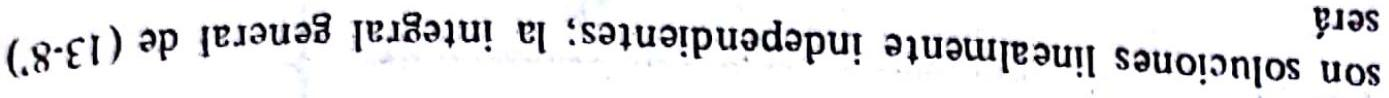
\includegraphics[max width=\textwidth, center]{2025_09_05_adecef5eb2053bc129b5g-331(8)}\\
$(6-\varepsilon \mathrm{I}) \quad(x)^{n} \Lambda^{\prime} \cdots{ }^{\prime}(x)^{2} X^{\prime}(x)^{1} X$\\
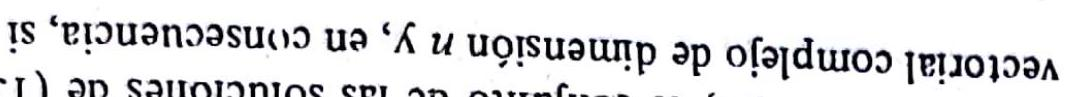
\includegraphics[max width=\textwidth, center]{2025_09_05_adecef5eb2053bc129b5g-331(3)}\\
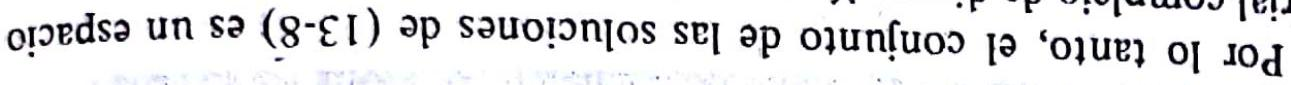
\includegraphics[max width=\textwidth]{2025_09_05_adecef5eb2053bc129b5g-331(5)} นา о เวอยdsa [ว $\Lambda$ ' ( $8-\varepsilon I$ ) บวอยJS! เยs\\
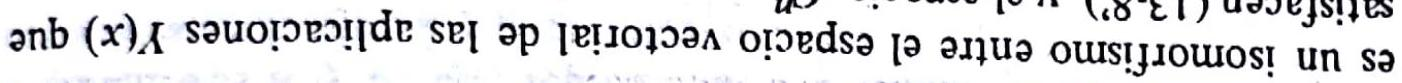
\includegraphics[max width=\textwidth, center]{2025_09_05_adecef5eb2053bc129b5g-331(10)}

$$
x \leftarrow(x)_{X}
$$

иотэвว![de р] әnb ләл soưәроd ' $u$ иәрло әр [とәи![ [ए!ว\\
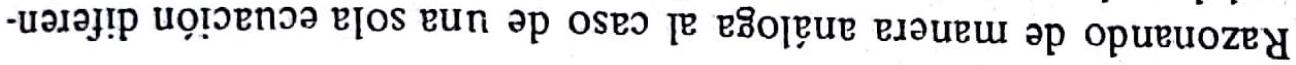
\includegraphics[max width=\textwidth, center]{2025_09_05_adecef5eb2053bc129b5g-331(1)}\\
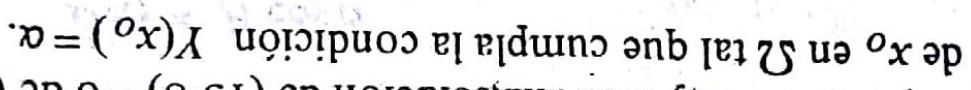
\includegraphics[max width=\textwidth, center]{2025_09_05_adecef5eb2053bc129b5g-331(7)}\\
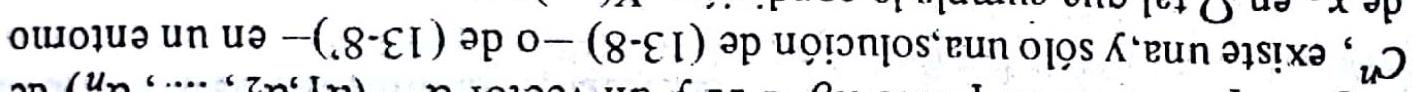
\includegraphics[max width=\textwidth, center]{2025_09_05_adecef5eb2053bc129b5g-331}\\
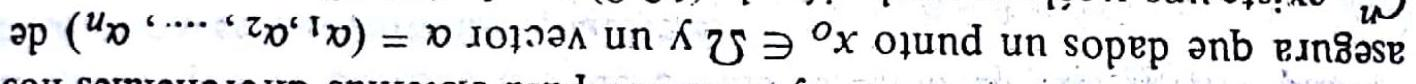
\includegraphics[max width=\textwidth, center]{2025_09_05_adecef5eb2053bc129b5g-331(4)}\\
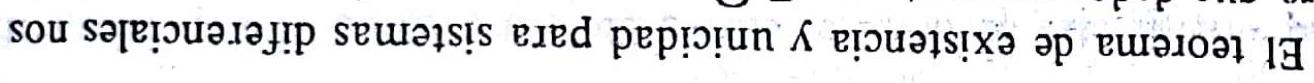
\includegraphics[max width=\textwidth, center]{2025_09_05_adecef5eb2053bc129b5g-331(2)}\\
(8-દI) IEłuวSaIdәI e.xed\\
(. $8-\varepsilon \mathrm{I}$ )

$$
(x)_{X}(x)_{V}=(x)_{C}
$$

sourspuod\\
'(8-EI) әр sәциә!!yәол sol sod epreunof zingur el sa $(x) V$ !S

$$
u \mathcal{D}^{\text {แ } \vartheta} \mho \text { әр }\left[(x)^{u} K^{\prime} \cdots(x)^{\prime} K\right] \leftarrow x
$$

$(x)_{X}$ นọlovo! $\mathrm{d}^{\mathrm{d} \mathrm{e}}$ ణ]\\
Opuriәр!Suos e1วeduos sęu eurof eun ọeq ( $8-\varepsilon 1$ ) sourresәrdxy\\
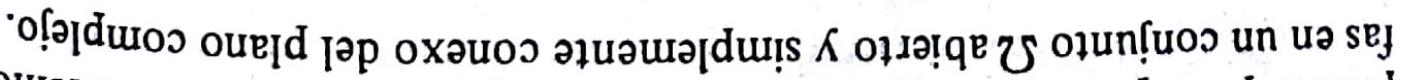
\includegraphics[max width=\textwidth, center]{2025_09_05_adecef5eb2053bc129b5g-331(6)}\\
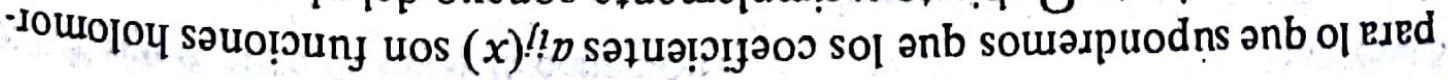
\includegraphics[max width=\textwidth, center]{2025_09_05_adecef5eb2053bc129b5g-331(9)}

Si cada una de las (13-9) es de la forma

$$
Y_{k}(x)=\left[y_{1 k}(x), y_{2 k}(x), \ldots, y_{n k}(x)\right] \text { para } 1 \leqslant k \leqslant n,
$$

su independencia lineal equivale a que el determinante

\[
\left|\begin{array}{cccc}
y_{1}^{1}(x) & y_{1}^{2}(x) & \ldots & y_{1}^{n}(x)  \tag{13-10}\\
\ldots \ldots \ldots \ldots \ldots \ldots \ldots \ldots \ldots \ldots \ldots \ldots \ldots \ldots \ldots \ldots \ldots \ldots \ldots \ldots \ldots \ldots \ldots \ldots \ldots \ldots \ldots & y_{n}^{n}(x)
\end{array}\right|
\]

sea no nulo en $\Omega$.\\
Procediendo de manera análoga a lo hecho en el teorema 3 del parágrafo 6 podemos demostrar que es nulo en $\Omega$ si, y sólo si, existe un punto $a \in \Omega$ en que lo sea.

Diremos que un sistema diferencial lineal es no homogéneo si tiene la forma


\begin{equation*}
Y^{\prime}-A(x) Y=B, \tag{13-11}
\end{equation*}


donde $B$ es una aplicación

$$
x \rightarrow\left[b_{1}(x), b_{2}(x), \ldots, b_{n}(x)\right]
$$

de $\Omega$ en $C^{n}$.\\
Podemos extender a este caso todos los resultados válidos para las ecuaciones lineales. Por ejemplo, la solución general de un sistema no homogéneo será la suma de una solución particular y de la solución general del homogéneo.

También es posible extender al caso de los sistemas (13-11) los métodos ya conocidos para el cálculo de soluciones particulareş.

Veamos ahora el caso en que $B=0$ y la matriz $A(x)$ tiene elementos constantes, es decir, el de sistemas


\begin{equation*}
Y^{\prime}(x)=A \quad Y(x), \tag{13-12}
\end{equation*}


llamados de coeficientes constantes.\\
Supongamos entonces que (13-12) admite soluciones de la forma


\begin{equation*}
Y(x)=e^{r x} y_{0} \tag{13-13}
\end{equation*}


donde $r$ es un número complejo e $y_{0}=\left(\alpha_{1}, \alpha_{2}, \ldots, \alpha_{n}\right)_{1}$ un vector de $C^{n}$.\\
Derivando obtenemos $Y^{\prime}(x)=r e^{r x} y_{0}$ y reemplazando en (13-12) es

$$
r e^{r x} y_{0}=A e^{r x} y_{0}=e^{r x} A y_{0}
$$

De otra manera, el número $r$ y el vector $y_{0}$ deben ser tales que


\begin{equation*}
A y_{0}=r y_{0} \tag{13-14}
\end{equation*}


La igualdad anterior prueba que (13-13) es solución de (13-12) si, y sólo si, $r$ es autovalor de la matriz $A$, con autovector $y_{0}$.

También podemos probar --no lo haremos-- que podemos obtener una base de soluciones del sistema si la matriz $A$ admite $n$ autovalores distintos. Si esto no sucede el método anterior puede emplearse efectuando algunas modificaciones.

Finalmente observemos que siempre es posible reducir el sistema a una sola ecuación aumentando su orden.

\section*{Ejemplo}
Sea el sistema

$$
\left\{\begin{array}{l}
y^{\prime}=y+4 z \\
z^{\prime}=2 y-z
\end{array}\right.
$$

de dos funciones incógnitas $y(x), z(x)$.\\
La matriz de sus coeficientes es

$$
A=\left(\begin{array}{cc}
1 & 4 \\
2 & -1
\end{array}\right)
$$

cuyos autovalores son las raíces de la ecuación

$$
\operatorname{det}\left(\begin{array}{cc}
1-r & 4 \\
2 & -1-r
\end{array}\right)=r^{2}-9=0
$$

es decir, $r_{1}=3$ y $r_{2}=-3$. Los autovectores correspondientes son

$$
V_{1}=(2 \alpha, \alpha) \quad, \quad V_{2}=(\beta,-\beta) .
$$

La solución general busčada resulta $(y, z)=e^{3 x} V_{1}+e^{-3 x} V_{2}$ o sea

$$
\left\{\begin{array}{l}
y(x)=2 \alpha e^{3 x}+\beta e^{-3 x}, \\
z(x)=\alpha e^{3 x}-\beta e^{-3 x}
\end{array}\right.
$$

\section{Ecuaciones en derivadas parciales casilineales de primer orden}
Diremos que una ecuación en derivadas parciales es casilineal de primer orden si es de la forma


\begin{equation*}
F_{1}\left(x_{1}, \ldots, x_{n}, y\right) \frac{\partial y}{\partial x_{1}}+\cdots+F_{n}\left(x_{1}, \ldots, x_{n}, y\right) \frac{\partial y}{\partial \dot{x}_{m}}=G\left(x_{1}, \ldots, x_{n}, y\right) \tag{14-1}
\end{equation*}


es decir, si es lineal con respecto a las derivadas parciales de la función incógnita $y\left(x_{1}, \ldots, x_{n}\right)$ aunque puede no serlo con respecto a ella misma.

Haremos un tratamiento geométrico del problema limitándonos al caso $n=2$ es decir a la ecuación



\begin{equation*}
F_{1}(x, y, z) \frac{\partial \varphi}{\partial x}+F_{2}(x, y, z) \frac{\partial \varphi}{\partial y}=G(x, y, z) . \tag{14-2}
\end{equation*}


Suponiendo que las funciones $F_{1}, F_{2}$ y $G$ son continuas y no simul. táneamente nulas en un abierto $U$ del espacio.

Si consideramos el campo vectorial

$$
\vec{V}(x, y, z)=F_{1}(x, y, z) \vec{i}+F_{2}(x, y, z) \vec{y}+G(x, y, z) \vec{k},
$$

y tenemos en cuenta que las soluciones de (14-2) son superficies $z=\varphi(x, y)$, probaremos el siguiente

\section*{Teorema}
Una superficie S de ecuación $\mathrm{z}=\varphi(\mathrm{x}, \mathrm{y})$ es solución de (14-2) si, $y$ sólo si, es una superficie vectorial del campo V; es decir, si, y sólo si, S contiene a todas las lineas de fuerza del campo V que pasen por alguno de sus puntos.\\
a) Supongamos que $S$ sea una superficie vectorial del campo $V$; es decir, que si $P=\left(x_{0}, y_{0}, z_{0}\right)$ es un punto de $S$, y $\Gamma$ una línea de fuerza que pasa por $P$, entonces debe ser $\Gamma \subseteq S$. Luego, la recta tangente a $\Gamma$ en $P$ y la recta normal a $S$ en $P$ deben ser perpendiculares.

Como $\Gamma$ es una línea de fuerza, el vector

$$
\left[F_{1}(P), F_{2}(P), G(P)\right]
$$

es tangente a $\Gamma$ en $P$.\\
El vector

$$
\left[\frac{\partial \varphi}{\partial x}\left(x_{0}, y_{0}\right), \frac{\partial \varphi}{\partial y}\left(x_{0}, y_{0}\right),-1\right]
$$

es normal a $S$ en $P$ y por lo tanto su producto escalar con el anterior debe ser nulo

$$
F_{1}\left(x_{0}, y_{0}, z_{0}\right) \frac{\partial \varphi}{\partial x}\left(x_{0}, y_{0}\right)+F_{2}\left(x_{0}, y_{0}, z_{0}\right) \frac{\partial \varphi}{\partial y}\left(x_{0} y_{0}\right)=G\left(x_{0}, y_{0}, z_{0}\right)
$$

Como $P$ es arbitrario, esto prueba que $z=\varphi(x, y)$ es solución de (14-2) en todo el abierto $U$.\\
b) Llamemos $S$ a la superficie de ecuación $z=\varphi(x, y)$ y supongamos que $\varphi$ satisface la ecuación (14-2). Sea $P=\left[x_{0}, y_{0}, \varphi\left(x_{0}, v_{0}\right)\right]$ un punto de $S$, y $P^{\prime}=\left(x_{0} y_{0}\right)$ su proyección sobre el plano $X Y$.

Sea $\Gamma$ ' la curva plana que pasa por $\left(x_{0}, y_{0}^{\prime}\right)$ y que satisface la ecuación diferencial


\begin{equation*}
\frac{d x}{F_{1}[x, y, \varphi(x, y)]}=\frac{d y}{F_{2}[x, y, \varphi(x, y)]} . \tag{14-3}
\end{equation*}


Como esta igualdad equivale a

$$
\frac{\frac{\partial \varphi}{\partial x} d x}{\frac{\partial \varphi}{\partial x} F_{1}[x, y, \varphi(x, y)]}=\frac{\frac{\partial \varphi}{\partial y} d y}{\frac{\partial \varphi}{\partial y} F_{2}[x, y, \varphi(x, y)]}
$$

y de ella puede obtenerse


\begin{gather*}
\frac{d x}{F_{1}[x, y \cdot \varphi(x, y)]}=\frac{d y}{F_{2}[x, y, \varphi(x, y)]}= \\
=\frac{\frac{\partial \varphi}{\partial x} d x+\frac{\partial \varphi}{\partial y} d y}{\frac{\partial \varphi}{\partial x} F_{1}[x, y, \varphi(x, y)]+\frac{\partial \varphi}{\partial y} F_{2}[x, y, \varphi(x, y)]} \tag{14-4}
\end{gather*}


Deducimos así que si $\Gamma$ es la curva sobre $S$ cuya proyección sobre el plano $X Y$ es $\Gamma^{\prime}$, para los puntos de $\Gamma^{\top}$ se satisface

$$
z=\varphi(x, y),
$$

y también la (14-4), que por lo tanto podemos poner en la forma


\begin{equation*}
\frac{d x}{F_{1}(x, y, z)}=\frac{d y}{F_{2}(x, y, z)}=\frac{d z}{G(x, y, z)} . \tag{14.5}
\end{equation*}


Esto prueba que $\Gamma$ es una línea de fuerza del campo $\vec{V}$ que pasa por $P$ y está totalmente contenida en $S$.

Toda línea de fuerza que pase por $P$ debe coincidir con $\Gamma$, en virtud 'del teorema que nos da la unicidad de la solución de (14-5).

En consecuencia $S$ resulta unà superficie vectorial del campo $\vec{V}$.\\
Las soluciones de (14-2) pueden obtenerse entonces de la siguiente manera: se resuelve (14-5) expresando su integral general en la forma

\[
\left\{\begin{array}{l}
\Phi_{1}(x, y, z, \alpha, \beta)=0,  \tag{14-6}\\
\Phi_{2}(x, y, z, \alpha, \beta)=0,
\end{array}\right.
\]

que representa una familia de curvas en el espacio.\\
Si ahora establecemos una dependencia continua


\begin{equation*}
\Psi(\alpha, \beta)=0 \tag{14-7}
\end{equation*}


entre los parámetros, la familia uniparamétrica que resulta de (14-6) es una superficie $S$ cuya ecuación obtendremos eliminando $\alpha$ y $\beta$ del sistema formado por (14-6) y (14-7).

La superficie $S$ es solución de (14-2), ya que está constituida por líneas de fuerza de $\vec{V}$.

En la práctica resulta más conveniente tener la integral general de (14-5) en la forma

$$
\left\{\begin{array}{l}
u(x, y, z)=\alpha, \\
\nu(x, y, z)=\beta,
\end{array}\right.
$$

que puede obtenerse a partir del sistema (14-6), resolviéndolo respecto de las variables $\alpha$ y $\beta$. Si $\psi$ es entonces continua y con derivadas primeras continuas, la solución general de (14-2) tendrá entonces la forma

$$
\psi[u(x, y, z), v(x, y, z)]=0
$$

Si $\psi$ no es implícita, sino que adopta la forma $\beta=\varphi(a)$, la integral general es

$$
v(x, y, z)=\varphi[u(x, y, z)] .
$$

El procedimiento anterior de resolución de (14-2) puede justificarse analíticamente cualquiera sea el número de variables contenidas en la ecuación.

Este se precisa en el siguiente resultado, que no demostraremos:

\section*{Teorema}
Supongamos que

$$
F_{1}\left(x_{1}, \ldots, x_{n}, u\right) \frac{\partial u}{\partial x_{1}}+\cdots+F_{n}\left(x_{1}, \ldots, x_{n}, u\right) \frac{\partial u}{\partial x_{n}}=G\left(x_{1}, \ldots, x_{n}, u\right)
$$

es una ecuación casilineal en las derivadas parciales de primer orden de la función incógnita $\mathrm{u}\left(\mathrm{x}_{1}, \mathrm{x}_{2}, \ldots, \mathrm{x}_{\mathrm{n}}\right)$.

Entonces su integral general es de la forma

$$
\psi\left[u_{1}\left(x_{1}, \ldots, x_{n}\right), \ldots, u_{n}\left(x_{1}, \ldots, x_{n}\right)\right]=0
$$

donde las funciones


$$
\left\{\begin{array}{l}
u_{1}\left(x_{1}, \ldots, x_{n}\right)=\alpha_{1}, \\
u_{2}\left(x_{1}, \ldots, x_{n}\right)=\alpha_{2}, \\
\ldots \ldots \ldots \ldots \ldots \ldots \ldots \ldots \ldots \ldots \ldots \ldots \ldots \ldots \\
u_{n}\left(x_{1}, \ldots, x_{n}\right)=\alpha_{n},
\end{array}\right.
$$

son una base de soluciones del sistema diferencial


\begin{align*}
& \frac{d x_{1}}{F_{1}\left(x_{1}, \ldots, x_{n}, u\right)}=\frac{d x_{2}}{F_{2}\left(x_{1}, \ldots, x_{n}, u\right)}=\cdots= \\
& =\frac{d x_{n}}{F_{n}\left(x_{1}, \ldots, x_{n}, u\right)}=\frac{d u}{G\left(x_{1}, \ldots, x_{n}, u\right)} \tag{14-8}
\end{align*}


$y$ donde $\psi$ es una función arbitraria con derivadas primeras continuas.

\section*{OBSERVACION}
Si alguno de los coeficientes $F_{i}\left(x_{1}, \ldots, x_{n}, u\right)$ que aparecen en (14-8) es nulo, la igualdad debe interpretarse como exigiendo la supresión del cociente correspondiente, agregando además la ecuación $d x_{i}=0$.

\subsection{Ejemplos}
$1^{0}$ ) Resolvamos la ecuación casilineal de primer orden


\begin{equation*}
x^{2} \frac{\partial z}{\partial x}+y^{2} \frac{\partial z}{\partial y}=(x+y) z \tag{14-9}
\end{equation*}


las lineas de fuerza del campo

$$
V(x, y, z)=x^{2} \vec{i}+y^{2} \vec{j}+(x+y) z \vec{k}
$$

serán las soluciones del sistema diferencial

\section*{ECUACIONES DIFERENCIALES}
$$
\frac{d x}{x^{2}}=\frac{d y}{y^{2}}=\frac{d z}{(x+y) z}
$$

La integración de la primera ecuación nos da

$$
\frac{1}{x}-\frac{1}{y}=\alpha
$$

Como la zgunda se puede poner en la forma

$$
\frac{d y-d x}{y^{2}-x^{2}}=\frac{d z}{z(x+y)}
$$

o bien

$$
\frac{d(y-x)}{y-x}=\frac{d z}{z} ;
$$

su integral resulta

$$
\frac{z}{y-x}=\beta .
$$

Luego la integral general (14-9) es


\begin{equation*}
\psi\left(\frac{y-x}{x y}, \frac{z}{y-z}\right)=0 \tag{14-10}
\end{equation*}


en donde $\psi$ es una relación arbitraria entre los parámetros $\alpha$ y $\beta$.\\
La integral general de una ecuación en derivadas parciales puede presentarse bajo formas distintas.

Por ejemplo, a partir de


$$
\frac{1}{x}-\frac{1}{y}=\alpha \quad, \quad \frac{z}{y-x}=\beta
$$

de finimos el parámetro $\gamma=\alpha . \beta$. Entonces la integral general de (14-9) puede escribirse en la forma

$$
z=x y \Phi\left(\frac{y-x}{x y}\right)
$$

\section*{OBSERVACION}
Con este primer resultado ya encontramos la diferencia, de gran importancia, entre ecuaciones diferenciales ordinarias y en derivadas parciales. En las primeras la integral general depende de los valores numéricos de uno o varios parámetros. En la integral general de la ecuación en derivadas parciales que acabamos de obtener aparecen funciones arbitrarias.\\
$2^{0}$ ) Sea la ecuación

$$
a \frac{\partial z}{\partial x}+b \frac{\partial z}{\partial y}=0
$$

con $a$ y $b$ constantes no nulas. Para resolverla consideramos el sistema diferencial

$$
\left\{\begin{array}{l}
\frac{d x}{a}=\frac{d y}{b} \\
d z=0
\end{array}\right.
$$

cuya integral general es

$$
\left\{\begin{array}{l}
b x-a y=\alpha, \\
z=\beta .
\end{array}\right.
$$

Por lo tanto las soluciones de (14-5) son rectas paralelas al plan0\\
$z=0$, cuyos cosenos directores son múltiplos de los números $a, b$ y 0 ; ${ }_{0}$ sea rectas paralelas a la recta $\Delta$ de ecuaciones

$$
\Delta:\left\{\begin{array}{l}
b x-a y=0 \\
z=0
\end{array}\right.
$$

La integral general --de acuerdo con el teorema anterior- tendrá la forma

$$
z=\varphi(b x-a y)
$$

con $\varphi$ una función arbitraria. Entonces las soluciones son cilindros generales, que tienen como curvas directrices a las de ecuación $z=\varphi(x)$ contenidas en el plano $X Z$, y cuyas generatrices son paralelas a la recta $\Delta$.\\
$3^{0}$ ) Finalmente, consideremos la ecuación en derivadas parciales


\begin{equation*}
(y-z) \frac{\partial u}{\partial x}+(z-x) \frac{\partial u}{\partial y}+(x-y) \frac{\partial u}{\partial z}=0 . \tag{14-11}
\end{equation*}


El sistema diferencial (14-8) asociado es

\[
\left\{\begin{array}{l}
\frac{d x}{y-z}=\frac{d y}{z-x}=\frac{d z}{x-y}  \tag{14-12}\\
d u=0
\end{array}\right.
\]

Como la suma de todos los denominadores del sistema es nula, debe serlo también la de los numeradores; luego

$$
d x+d y+d z=0
$$

Operando de la misma manera sobre el sistema


$$
\left\{\begin{array}{l}
\frac{x d x}{x y-x z}=\frac{y d y}{y z-x y}=\frac{z d z}{x z-y z} \\
d u=0
\end{array}\right.
$$

equivalente a (14-12), resulta

$$
x d x+y d y+z d z=0
$$

De aquí, la integral general del sistema es

$$
\left\{\begin{array}{l}
x+y+z=\alpha, \\
x^{2}+y^{2}+z^{2}=\beta, \\
u=\gamma .
\end{array}\right.
$$

Luego, la solución general de (14-11) se escribe

$$
u=\Phi\left(x+y+z, x^{2}+y^{2}+z^{2}\right)
$$

a partir de $\gamma=\Phi(\alpha, \beta)$.\\
Para determinar integrales particulares de una ecuación diferencial ordinaria es necesario dar la condición inicial de que la curva pasa por un punto ( $x_{0}, y_{0}$ ) del plano.

En cambio, cuando se trata de una ecuación en derivadas parciales, la condición inicial no es numérica, sino funcional.

Limitándonos al caso de una ecuación casilineal (14-2), el problema de resolverla con una condición inicial se denomina problema de Cauchy', y se enuncia de la manera siguiente:

Dadas la ecuación (14-2) y una curva $\Gamma$ del espacio que no sea solución del sistema diferencial (14-5), se pide hallar la única superficie $S$, solución de la ecuación tal que $\Gamma \subset S$.

Como por cada punto de $\Gamma$ pasa una única línea de fuerza, la superficie $S$ estará formada por todas las líneas de fuerza soluciones de (14-5) que corten a $\Gamma$.

Obsérvese que si $\Gamma$ es una línea de fuerza del campo $\vec{V}$, asociado a la ecuación, entonces la superficie $S$ puede no ser única. Basta verlo tomando $\Gamma=\Delta$ en el segundo ejemplo. Entonces, cualquier función $\varphi$ que cumpla $\varphi(0)=0$ nos proporcionará una superficie solución de la ecuación propuesta.

Si la curva I'está dada por

\[
\left\{\begin{array}{l}
f(x, y, z)=0  \tag{14-13}\\
g(x, y, z)=0
\end{array}\right.
\]

la relación que debe establecerse entre los parámetros $\alpha$ y $\beta$ de (14-6), para que la superficie pase por $\Gamma$, es la siguiente: $\alpha$ y $\beta$ deben ser tales que (146) y (14-13) se satisfagan simultáneamente. Eliminando $x, y, z$ de este sistema conjunto resulta la ecuación


\begin{equation*}
F(\alpha, \beta)=0 . \tag{14-14}
\end{equation*}


Si finalmente se eliminan $\alpha$ y $\beta$ del sistema formado por (14-6) y (14-14) tenemos la ecuación de $S$ en la forma

$$
X(x, y, z)=0
$$

\section*{Ejemplo}
Hallar la ecuación de la superficie $S$ solución de


\begin{equation*}
\left(3 z^{2}+z\right)\left(\frac{\partial z}{\partial x}+\frac{\partial z}{\partial y}\right)=x+y \tag{14-15}
\end{equation*}


que pasa por la circunferencia

$$
\left\{\begin{array}{l}
x^{2}+y^{2}=1 \\
z=1
\end{array}\right.
$$

Resolvemos el sistema


$$
\frac{d x}{3 z^{2}+z}=\frac{d y}{3 z^{2}+z}=\frac{d z}{x+y} .
$$

La primera ecuación se escribe $d x=d y$ y tiene solución


\begin{equation*}
x=y+\alpha_{\bullet} . \tag{14-16}
\end{equation*}


Reemplazando en la segunda obtenemos

$$
(2 x-\alpha) d x=\left(3 z^{2}+z\right) d z,
$$

que integrada es


\begin{equation*}
2 x^{2}-2 \alpha x+\beta=2 z^{3}+z^{2} . \tag{14-17}
\end{equation*}


Eliminando $x, y, z$ del sistema

$$
\left\{\begin{array}{l}
2 z^{3}+z^{2}=2 x^{2}-2 \alpha x+\beta \\
y=x-\alpha \\
x^{2}+y^{2}=1 \\
z=1
\end{array}\right.
$$

resulta $\beta-\alpha^{2}=2$.\\
Como hay que eliminar $\alpha$ y $\beta$ entre esta ecuación, (14-16) y (14-17) llegamos a

$$
x^{2}+y^{2}+2=2 z^{3}+z^{2}
$$

Si $\Gamma$ viene dada por sus ecuaciones paramétricas, un razonamiento análogo nos muestra que (14-14) se obtiene eliminando $t$ en el sistema

$$
\begin{aligned}
& \Phi_{1}[x(t), y(t), z(t), \alpha, \beta]=0 ; \\
& \Phi_{2}[x(t), y(t), z(t), \alpha, \beta]=0 .
\end{aligned}
$$

\section{Ecuaciones en derivadas parciales}
Este parágrafo tiene como objeto dar algunos métodos de resolución, casi siempre el de separación de variables, de problemas de contorno para las ecuaciones en derivadas parciales más usadas en las aplicaciones.

Consideraremos sólo ecuaciones lineales de segundo orden, es decir de la forma


\begin{equation*}
\sum_{i, j=1}^{n+1} A_{i j} \frac{\partial^{2} u}{\partial x_{i} \partial x_{J}}+\sum_{i=1}^{n+1} B_{i} \frac{\partial u}{\partial x_{i}}+C u=F, \tag{15-1}
\end{equation*}


donde la función incógnita $u$ y los coeficientes $A_{i j}, B_{i}, C$ y $F$ dependen de las $n+1$ variables reales $x_{1}, \ldots, x_{n+1}$.

Por ser la ecuación (15-1) lineal, su integral general se obtiene sumando a la solución general de la ecuación homogénea, una solución particular de la no homogénea.

En nuestro estudio nos limitaremos al caso homogéneo, o sea cuando $F=0$.

El concepto de integral general tiene menos importancia que en el caso de las ecuaciones diferenciales ordinarias. En efecto, en el parágrafo 14 se probó que la solución general de las ecuaciones de primer orden depende de funciones arbitrarias.

Esto también ocurre con las ecuaciones de orden superior.\\
Por ejemplo, la integral general de

$$
\frac{\partial^{2} z}{\partial x \partial y}=0
$$

es

$$
z\left(x, y^{\prime}\right)=\alpha(x)+\beta(y),
$$

donde $\alpha$ y $\beta$ son funciones derivables cualesquiera.\\
No siempre es posible obtener a partir de la integral general soluciones que verifiquen determinadas condiciones. Más aún: salvo en casos particulares tampoco se pueden obtener las integrales generales.

\section*{MATEMATICA AVANZADA PARA LA FIBICA}
Por esta razón, es preferible buscar no una solución general, sino una familia de soluciones dependiente de ciertos parámetros.

Estos parámetros pueden ser discretos o continuos.\\
En el primer caso, la familia se escribe como

$$
\left\{u_{i_{1}, \ldots, i_{r}}\left(x_{1}, \ldots, x_{n+1}\right)\right\} i_{1, \ldots, i_{r}}=1,2, \ldots
$$

y a partir de ella se busca una solución de la forma sumatoria múltiple:

$$
\sum_{i_{k}=1}^{\infty} A_{i_{1}, \ldots, i_{r}} \cdot u_{i_{1}, \ldots, i_{r}}\left(x_{1}, \ldots, x_{n+1}\right) \quad \text { para } k=1,2, \ldots, r . \text { (15-2) }
$$

En cambio, si los parámetros que describen a la familia de soluciones son continuos, por ejemplo $r$ variables reales ( $\alpha_{1}, \ldots, \alpha_{r}$ ) que toma valores en un subconjunto $\Omega \subset R^{r}$, suponiendo que la familia es

$$
\left\{u\left(x_{1}, \ldots, x_{n}, \alpha_{1}, \ldots, \alpha_{r}\right)\right\}\left(a_{1}, \ldots, a_{r}\right) \in \Omega
$$

se plantea una solución


\begin{equation*}
\int_{\Omega} f\left(\alpha_{1}, \ldots, \alpha_{r}\right) u\left(x_{1}, \ldots, x_{n}, \alpha_{1}, \ldots, \alpha_{r}\right) d \alpha_{1} \ldots d \alpha_{r} \tag{15-3}
\end{equation*}


Tanto los coeficientes numéricos $A_{i_{1} \ldots, i_{r}}$ comola función $f\left(\alpha_{1}, \ldots, \alpha_{r}\right)$ se determinan de manera que (15-2) y (15-3), además de satisfacer la ecuación diferencial, cumplan las condiciones impuestas en el problema.

Este es el llamado método de superposición de soluciones, cuya aplicación exige que sea posible derivar bajo el signo de suma o de integración.

Aceptaremos que esto se verifica en todos los casos que vamos a analizar.

Las distintas condiciones que pueden imponerse a la solución de una ecuación en derivadas parciales, dan origen a dos tipos fundamentales de problemas: el problema de Cauchy y el problema de Dirichlet, que trataremos en el caso más simple.

Consideremos una ecuación de la forma (15-1), homogénea, que escribiremos abreviadamente $D u=0$. Supondremos que $u$ es función de\\
las $n+1$ variables $x_{1}, \ldots, x_{n}, t$.\\
El problema de Cauchy consiste en hallar una solución $u_{0}$ de la ecuación en un entorno de $t=0$, que cumpla las condiciones iniciales

\[
\left.\begin{array}{l}
u_{0}\left(x_{1}, \ldots, x_{n}, 0\right)=f\left(x_{1}, \ldots, x_{n}\right)  \tag{15-4}\\
\frac{\partial u_{0}}{\partial t}\left(x_{1}, \ldots, x_{n}, 0\right)=g\left(x_{1}, \ldots, x_{n}\right)
\end{array}\right\}
\]

Si la ecuación no contiene la derivada segunda de $u$ respecto de $t$, y sí la derivada primera, hay que suprimir la segunda de las condiciones (15-4).

Consideremos la ecuación (15-1) también homogénea, pero ahora función de las $n$ variables reales $x_{1}, \ldots, x_{n}$. Sea $\Omega$ un abierto de $R^{n}$ y $\Gamma$ su frontera.

El problema de Dirichlet es encontrar una función $u_{0}$, que satisfaga la ecuación en $\Omega$ y cumpla la condición de contorno: $u_{0}$ restringida a $\Gamma$ igual a $h$, donde $h$ es una función definida sobre $\Gamma$.

Naturalmente, para que estos problemas admitan solución, deben agregarse hipótesis sobre las funciones que se dan como dato y sobre la frontera del abierto $\Omega$.

Estudiaremos ahora la resolución de algunos casos particulares de estos problemas.

\section*{ECUACION DE LA DIFUSION}
Se denomina ecuación de la difusión o del calor a la ecuación diferencial


\begin{equation*}
\frac{\partial^{2} u}{\partial x_{1}^{2}}+\cdots+\frac{\partial^{2} u}{\partial x_{n}^{2}}-\frac{1}{a^{2}} \frac{\partial u}{\partial t}=0 \quad \text { para } a>0 \tag{15-5}
\end{equation*}


Nos proponemos resolver por el método de superposición de soluciones el siguiente problema de Cauchy:

Encontrar una solución de (15-5) válida para $t \geqslant 0$ y que cumpla la condición inicial

$$
u\left(x_{1}, \ldots, x_{n}, 0\right)=f\left(x_{1}, \ldots, x_{n}\right) \quad \forall\left(x_{1}, \ldots, x_{n}\right) \in R^{n},
$$

siendo $f$ una función dada.\\
Como el método a emplear no depende del número de variables, haremos el cálculo para $n=1$.

Es decir, vamos a resolver la ecuación


\begin{equation*}
\frac{\partial^{2} u}{\partial x^{2}}-\frac{1}{a^{2}} \frac{\partial u}{\partial t}=0 \tag{$15\cdot6$}
\end{equation*}


con la condición inicial

$$
u(x, 0)=f(x)
$$

Para ello observemos que la función


\begin{equation*}
u(x, t, \xi)=\frac{1}{\sqrt{t}} e^{-\frac{(x-\xi)^{2}}{4 a^{2} t}} \tag{15-7}
\end{equation*}


satisface la ecuación (15-5) para cualquier $\xi \in R$.\\
En efecto, basta derivar la función $u$ y comprobar que se cumple (15-6).

Superponiendo la familia de soluciones

$$
\{u(x, t, \xi)\}_{\xi \in R}
$$

obtenemos la función


\begin{equation*}
u(x, t)=\int_{-\infty}^{\infty} F(\xi) \cdot \frac{1}{\sqrt{t}} e^{-\frac{(x-\xi)^{2}}{4 a^{2} t}} d \xi \tag{15-8}
\end{equation*}


que es solución de (15-6), suponiendo que la función $F$ cumple las condiciones necesarias para asegurar la convergencia de la integral y la posibilidad de derivar bajo el signo de integración. Por el rápido decrecimiento\\
de la exponencial cuando $\boldsymbol{\xi}$ tiende a $\pm \infty$, esas condiciones se cumplen si $\boldsymbol{F}$ no crece demasiado rápidamente.

Es necesario ahora seleccionar la función $F$ de tal manera que se verifique la condición inicial.

Haciendo en (15-8) el cambio de variable $\xi=x+2 a t \lambda$, obtenemos

$$
u(x, t)=2 a \int_{-\infty}^{\infty} F(x+2 a \sqrt{t} \lambda) e^{-\lambda^{2}} d \lambda
$$

que para $t=0$ debe cumplir

$$
u(x, 0)=2 a F(x) \int_{-\infty}^{\infty} e^{-\lambda^{2}} d \lambda=f(x)
$$

Si tenemos en cuenta que $\int_{-\infty}^{\infty} e^{-\lambda^{2}} d \lambda$ vale $\sqrt{\pi}$, resulta

$$
F(x)=\frac{f(x)}{2 a \sqrt{\pi}},
$$

y entonces para asegurar que la integral converge $y$ que puede derivarse bajo el signo de integración, deben imponerse condiciones a la función $J$

Resulta entonces que el problema de Cauchy admite la solución

$$
\begin{aligned}
u(x, t) & =\frac{1}{2 a \sqrt{\pi t}} \int_{-\infty}^{\infty} f(\xi) e^{-\frac{(x-\xi)^{2}}{4 a^{2} t}} d \xi= \\
& =-\frac{1}{\sqrt{\pi}} \int_{-\infty}^{\infty} f(x+2 a \sqrt{t} \lambda) e^{-\lambda^{2}} d \lambda
\end{aligned}
$$

El caso de $n$ variables se trata de manera análoga usando la función

$$
u\left(x_{1}, \ldots, x_{n}, t, \xi_{1}, \ldots, \xi_{n}\right)=\frac{1}{t^{n_{1}^{2}}} e^{-\frac{\left(\xi_{1}-x_{1}\right)^{2}+\ldots+\left(\xi_{n}-x_{n}\right)^{2}}{4 a^{2} t}}
$$

que cs solución de $(15-5)$ para todo $\left(\xi_{1}, \ldots, \xi_{n}\right) \in R^{\prime \prime}$ y siguiendo el mismo razonamiento.

Vamos a estudiar otro problema de Cauchy relativo a la ecuación (15-6):

Se trata de encontrar una solución de esa ecuación definida en $0 \leqslant x \leqslant L, t \geqslant 0$ y que cumpla

\begin{enumerate}
  \item la condición inicial $u(x, 0)=f(x) \forall 0 \leqslant x \leqslant L$;
  \item las condiciones en los límites $u(0, t)=u(L, t)=0 \quad \forall t \geqslant 0$.
\end{enumerate}

Usaremos el metodo de separación de variables que consiste en buscar soluciones de la forma $u(x, t)=X(x) . T(t)$ y superponer luego las soluciones obtenidas.

Reemplazando en la ecuación (15-6) es

$$
X^{\prime \prime}(x) \cdot T(t)=\frac{1}{a^{2}} \quad X(x) \cdot T^{\prime}(t)
$$

o bien


\begin{equation*}
\frac{X^{\prime \prime}(x)}{X(x)}=\frac{1}{a^{2}} \frac{T^{\prime}(t)}{T(t)} . \tag{15.9}
\end{equation*}


El primer miembro de la igualdad (15-9) depende de $x$ y el segundo de $t$. Como se supone que ambas variables son independientes, resulta que debe existir una constante $\lambda$ tal clue

$$
\frac{X^{\prime \prime}}{X}=\lambda \quad \cdot \quad \frac{T^{\prime \prime}}{T}=a^{2} \lambda .
$$

Luego, cualquiera que sea $\lambda$. las soluciones de las ecuaciones diferenciales ordinarias

$$
\begin{aligned}
& X^{\prime \prime}-\lambda X=0, \\
& T^{\prime \prime}-a^{2} \lambda T=0,
\end{aligned}
$$

nos dan, al multiplicarlas, una solución de la ecuación en derivadas parcia. les (15-6). Ahora bien, las condiciones de contorno

$$
X(0) \cdot T(t)=X(L) \cdot T(t)=0 \quad \text { para } 0 \leqslant t
$$

exigen que $X$, además de verificar la ecuación diferencial $X^{\prime \prime}-\lambda X=0$, cumpla

$$
X(0)=X(L)=0
$$

Queda así planteado un problema del tipo Sturm-Liouville, cuyos autovalores y autovectores son. como ya vimos,

$$
\begin{array}{ll}
\lambda_{n}=-\left(\frac{n \pi}{L}\right)^{2} & \text { para } n=1,2, \ldots \\
X_{n}(x)=\operatorname{sen} \frac{n \pi}{L} x &
\end{array}
$$

Poniendo $\lambda=\lambda_{n}$, la ecuación diferencial

$$
T^{\prime}-a^{2} \lambda T=0
$$

admite la solución

$$
T(t)=e^{-\left(\frac{n \pi a}{L}\right)^{2}} t
$$

En resumen, cualquier función de la forma

$$
u_{n}(x, t)=e^{-\left(\frac{n \pi a}{L}\right)^{2}} t \operatorname{sen} \frac{n \pi}{L} x \quad \text { para } n=1,2 \cdots
$$

es solución de la ecuación (15-6) y cumple las condiciones en los límites.\\
Por lo tanto, bajo las hipótesis de convergencia que se requieran, la\\
función

$$
u_{n}(x, t)=\sum_{n=1}^{\infty} A_{n} e^{-\left(\frac{n \pi a}{L}\right)^{2} t} \operatorname{sen} \frac{n \pi}{L} x
$$

también verifica (15-6) y las condiciones en los límites. Para que $u$ cumpla la condición inicial debe ser

$$
f(x)=u(x, 0)=\sum_{n=1}^{\infty} A_{n} \operatorname{sen} \frac{n \pi}{L} x .
$$

$A_{n}$ resulta entonces el enésimo coeficiente del desarrollo de la función $f$ en serie de senos, en el intervalo $[0, L]$.

Es decir,

$$
A_{n}=\frac{2}{L} \int_{0}^{L} f(x) \operatorname{sen} \frac{n \pi}{L} x d x
$$

con lo que queda resuelto al problema.\\
La ecuación (15-6) en coordenadas polares es de la forma:


\begin{equation*}
\frac{\partial u}{\partial t}=k\left(\frac{\partial^{2} u}{\partial r^{2}}+\frac{1}{r} \frac{\partial u}{\partial r}\right) \quad \text { para } k>0 \tag{15-10}
\end{equation*}


Vamos a resolver para esta ecuación el siguiente problema:\\
Encontrar una función $u(r, t)$ definida en $0 \leqslant r \leqslant r_{0}$ que cumpla:

\begin{enumerate}
  \item es solución de (15-10) para $0 \leqslant r<r_{0}, t \geqslant 0$;
  \item satisface la condición en los límites $u\left(r_{0}, t\right)=0 \mathrm{~V} t \geqslant 0$ y la condición inicial $u(r, 0)=f(r)$.
\end{enumerate}

Aplicamos nuevamente el método de separación de variable, y escribimos $u(r, t)=R(r), T(t)$.

Razonando como antes, se llega a que existe una constante $\mu$ tal que

$$
\frac{T^{\prime}}{k T}=\frac{R^{\prime \prime}+\frac{1}{r} R^{\prime}}{R}=\mu
$$

Entonces $R$ debe ser solución de la ecuaciọn


\begin{equation*}
R^{\prime \prime}+\frac{1}{r} R^{\prime}-\mu R=0 \tag{$15\cdot11$}
\end{equation*}


Tomando $\mu=-\alpha^{2}, y$ mediante el cambio de variable $r \rightarrow \alpha . r$, (15-11) queda reducida a una ecuación de Bessel de orden cero, cuya integral general es

$$
A \cdot J_{0}(\alpha, r)+B \cdot N_{0}(\alpha r)
$$

Como la función de Neumann $N_{0}(\alpha, r)$ es no acotada para $r \rightarrow 0$, debe $\operatorname{ser} B=0$.

La condición $R\left(r_{0}\right)=0$ dice que debe ser

$$
\alpha=\alpha_{n}=\frac{\lambda_{n}}{r_{0}}
$$

donde $\left\{\lambda_{n}\right\}$ es la sucesión de ceros de $J_{0}(r)$.\\
Por lo tanto, la función

$$
u_{n}(r, t)=e^{-k \alpha_{n}^{2}} \quad J_{0}\left(\alpha_{n} . r\right) \quad \text { para } n=1,2, \ldots,
$$

es solución de (15-10) y cumple la condición en los límites.\\
Bajo ciertas hipótesis de convergencia, la superposición de soluciones

$$
u(r, t)=\sum_{n=1}^{\infty} A_{n} e^{-k a_{n}^{2} t} J_{0}\left(\alpha_{n} r\right)
$$

será solución del problema planteado si

$$
f(r)=\sum_{n=1}^{\infty} A_{n} J_{0}\left(\alpha_{n} r\right)
$$

Es decir, si $A_{n}$ es el enésimo coeficiente del desarrollo de $f(r)$ en serie de Fourier-Bessel:

$$
A_{n}=\frac{2}{r_{0}^{2}\left|J_{0}^{\prime}\left(\alpha_{n} r_{0}\right)\right|^{2}} \int_{0}^{r_{0}} r f(r) J\left(\alpha_{n} r\right) d r
$$

\section*{ECUACION DE LAS CUERDAS}
La ecuación de las cuerdas vibrantes es


\begin{equation*}
\frac{\partial^{2} u}{\partial x^{2}}-\frac{1}{c^{2}} \frac{\partial^{2} u}{\partial t^{2}}=0 \quad \text { para } .>0 \tag{$15\cdot12$}
\end{equation*}


Hagamos el cambio de variable $\xi=x+c t ; y=x-c t$.\\
Aplicando la regla de la derivación compuesta se tiene:

$$
\begin{gathered}
\frac{\partial u}{\partial x}=\frac{\partial u}{\partial \xi}+\frac{\partial u}{\partial y^{\prime}} ; \quad \frac{\partial u}{\partial t}=c \frac{\partial u}{\partial \xi}-c \frac{\partial u}{\partial y} . \\
\frac{\partial^{2} u}{\partial x^{2}}=\frac{\partial^{2} u}{\partial \xi^{2}}+2 \frac{\partial^{2} u}{\partial \xi \partial!}+\frac{\partial^{2} u}{\partial y^{\prime 2}} ; \quad \frac{\partial^{2} u}{\partial t^{2}}=c^{2}\left(\frac{\partial^{2} u}{\partial \xi^{2}}-2 \frac{\partial^{2} u}{\partial \xi \partial y^{\prime}}+\frac{\partial^{2} u}{\partial y^{2}}\right)
\end{gathered}
$$

Reemplazando en (15-12) resulta la ecuación

$$
4 \frac{\partial^{2} u}{\partial \xi \partial y}=0,
$$

cuya integral es $\alpha(\xi)+\beta(y)$, donde $\alpha$ y $\beta$ son funciones cualesquiera, derivables hasta el orden dos.

Luego, la integral general de (15-12) es


\begin{equation*}
u(x, t)=\alpha(x+c t)+\beta(x-c t) . \tag{15-13}
\end{equation*}


La ecuación (15-12) es uno de los casos particulares en que se puede encontrar fácilmente la solución general.

Ahora resolveremos a partir de (15-13) el siguiente problema de Cauchy:

Encontrar una solución de (15-12) válida para todo $x$ y para todo $t$, que satisfaga las condiciones iniciales

$$
u(x, 0)=f(x) \quad, \quad \frac{\partial u}{\partial t}(x, 0)=g(x)
$$

Se supondrá que $g(x)$ es una función localmente integrable.\\
De acuerdo con las condiciones impuestas, las funciones $\alpha$ y $\beta$ deben cumplir:


\begin{align*}
& \alpha(x)+\beta(x)=f(x) \\
& c\left[\alpha^{\prime}(x)-\beta^{\prime}(x)\right]=g(x) \tag{15-14}
\end{align*}


Integrando esta última igualdad se obtiene


\begin{equation*}
\alpha(x)-\beta(x)=\frac{1}{c} \int_{0}^{x} g(\tau) d \tau+K \tag{15-15}
\end{equation*}


A partir de (15-14) y (15-15) se despejan las funciones $\alpha(x)$ y $\beta(x)$ :

$$
\begin{aligned}
& \alpha(x)=\frac{1}{2}\left[f(x)+\frac{1}{c} \int_{0}^{x} g(\tau) d \tau+K\right] \\
& \beta(x)=\frac{1}{2}\left[f(x)-\frac{1}{c} \int_{0}^{x} g(\tau) d \tau-K\right]
\end{aligned}
$$

Luego la solución (15-13) puede escribirse en la forma $u(x, t)=\frac{1}{2}\left\{f(x+c t)+f(x-c t)+\frac{1}{c}\left[\int_{0}^{x+c t} g(\tau) d \tau-\int_{0}^{x-c t} g(\tau) d \tau\right]\right\}$ o equivalentemente:


\begin{equation*}
u(x, t)=\frac{f(x+c t)+f(x-c t)}{2}+\frac{1}{2 c} \int_{x-c t}^{x+c t} g(\tau) d \tau \tag{15-16}
\end{equation*}


Es interesante estudiar la forma en que esta solución depende de las condiciones iniciales:

En un punto $P=(x, t)$ del plano, la función (15-16) toma el valor

$$
u(P)=\frac{f(N)+f(M)}{2}+\frac{1}{2 c} \int_{M}^{N} g(\tau) d \tau
$$

\begin{figure}[h]
\begin{center}
  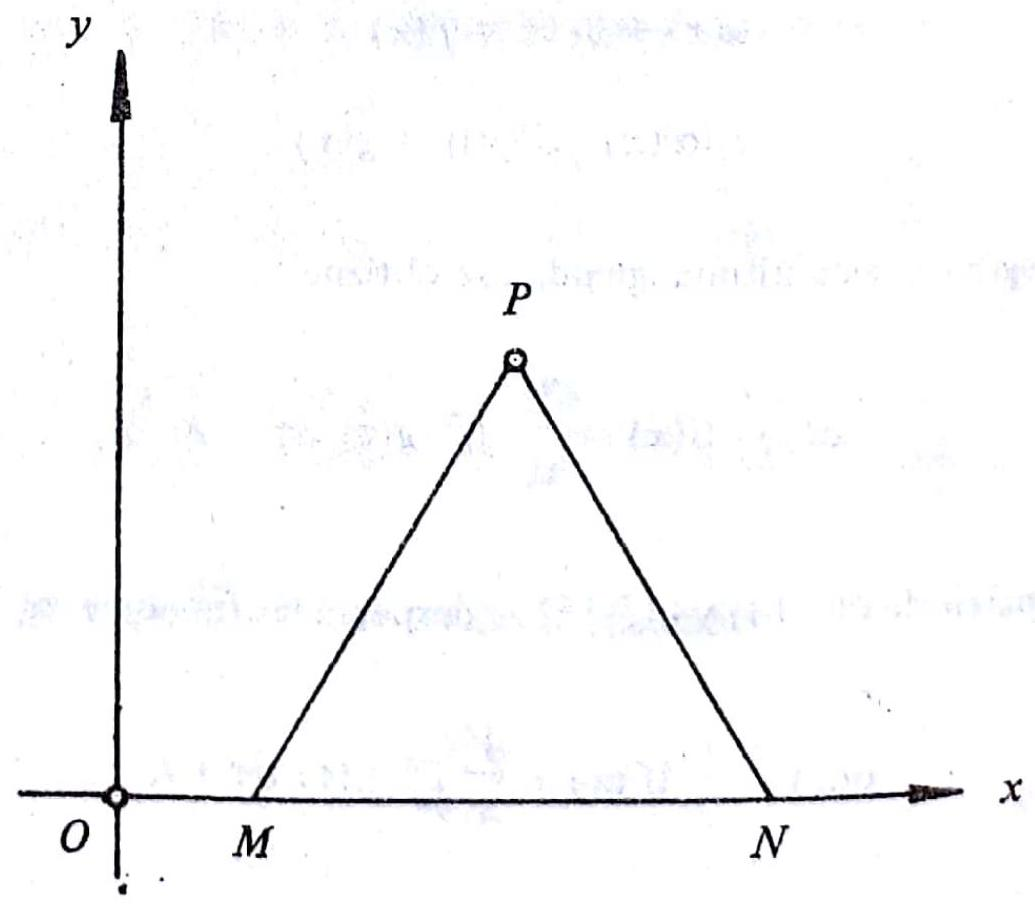
\includegraphics[width=\textwidth]{2025_09_05_adecef5eb2053bc129b5g-357}
\captionsetup{labelformat=empty}
\caption{Figura 16}
\end{center}
\end{figure}

donde $M$ y $N$ son los puntos $(x-c t, 0)$ y $(x+c t, 0)$, respectivamente.\\
Es decir, el valor de la función $u$ en el punto $P$ depende de los valores de $g$ en el segmento $\overline{M N}$ y de los de $f$ en $M$ y $N$.

Una variación de $f$ en los puntos $M$ o $N$ se propagará según las rectas $\overline{M P}$ o $\overline{N P}$, llamadas características de la ecuación.

El problema de Cauchy anterior, corresponde al caso de una cuerda libre de longitud infinita.

Si se supone ahora que la cuerda tiene un extremo fijo debe plantearse otro problema que es el siguiente:

Encontrar una solución de (15-12) válida para $x \geqslant 0$, y que verifique

\begin{enumerate}
  \item condición en los límites: $u(0, t)=0$;
  \item condiciones iniciales: $u(x, 0)=f(x), \frac{\partial u}{\partial t}(x, 0)=g(x)$.
\end{enumerate}

Debe ser entonces $f(0)=0$.\\
Prolonguemos $f$ y $g$ a toda la recta por imparidad, y llamemos $F$ y $G$ a esas prolongaciones. Entonces, según (15-16) la función


\begin{equation*}
u(x, t)=\frac{F(x+c t)+F(x-c t)}{2}+\frac{1}{2 c} \int_{x-c t}^{x+c t} G(\tau) d \tau \tag{15-17}
\end{equation*}


es solución de (15-12) y cumple la condición 1). Pero también verifica 2), pues teniendo en cuenta la imparidad de $F$ y $G$, es

$$
u(0, t)=\frac{F(c t)+F(-c t)}{2}+\frac{1}{2 c} \int_{-c t}^{c t} G(\tau) d \tau=0
$$

Luego (15-17) es la solución del problema planteado, para $x \geqslant 0$.\\
Una variante que se aplica en el estudio de los tubos sonoros, es la siguiente:

Encontrar una función $u(x, t)$, solución de (15-17) en $x \geqslant 0$, que cumpla


\begin{enumerate}
  \item condición en los límites: $\frac{\partial u}{\partial t}(0, t)=0$;
  \item condiciones iniciales: $u(x, 0)=f(x) ; \frac{\partial u}{\partial t}(x, 0)=g(x)$.
\end{enumerate}

Un cálculo análogo al anterior prueba que (15-17) es una solución del problema cuando $F$ y $G$ son las prolongaciones de $f$ y $g$ respectivamente, a toda la recta, por paridad.

El caso más importante es el de la cuerda vibrante con dos extremos fijos, que corresponde al siguiente problema de Cauchy:

\begin{enumerate}
  \item $u(x, t)$ debe ser solución de (15-17) en $C<x<l$, cumpliendo:
  \item condiciones en los límites: $u(0, t)=0 ; u(l, t)=0$;
  \item condiciones iniciales: $u(x, 0)=f(x) ; \frac{\partial u}{\partial t}(x, 0)=g(x)$.
\end{enumerate}

Vamos a resolver este problema por separación de variables.\\
Para simplificar, supondremos que en la ecuación (15-12), es $c=1$.\\
Buscamos una solución de la forma $u(x, t)=X(x) . T(t)$, que por lo tanto debe verificar

$$
\frac{X^{\prime \prime}}{X}=\frac{T^{\prime \prime \prime}}{T}=\lambda,
$$

para alguna constante $\lambda$.\\
Esto da origen a las dos ecuaciones

$$
\left\{\begin{array}{l}
X^{\prime \prime}-\lambda X=0 \\
T^{\prime \prime}-\lambda T=0
\end{array}\right.
$$

$X$ debe satistacer además las condiciones $X(0)=X(l)=0$.

Es decir, se obtiene un problema de Sturm-Liouville, análogo al que resultaba en la ecuación de la difusión.

Entonces sus autovalores y autovectores son, respectivamente:\\
$\lambda_{n}=-\left(\frac{n \pi}{l}\right)^{2} \quad ; X_{n}(x)=\operatorname{sen} \frac{n \pi}{l} x \quad$ para $n=1,2, \ldots$\\
Reemplazando $\lambda$ por $\lambda_{n}$ en la ecuación diferencial para $T$, resulta

$$
T_{n}(x)=A_{n} \cos \frac{n \pi}{l} t+B_{n} \operatorname{sen} \frac{n \pi}{l} t
$$

Si se multiplica $X_{n}$ por $T_{n}$, se obtiene una familia de soluciones $\left\{u_{n}(x, t)\right\}$, cuya superposición da\\
$u(x, t)=\sum_{n=1}^{\infty}\left[A_{n} \cos \frac{n \pi}{l} t+B_{n} \operatorname{sen} \frac{n \pi}{l} t\right] \operatorname{sen} \frac{n \pi}{l} x \cdot(15 \cdot 18)$

Para que esta función, además de ser solución de (15-12) y cumplir las condiciones iniciales satisfaga también las condiciones en los límites debe imponerse

$$
\begin{aligned}
& f(x)=u(x, 0)=\sum_{n=1}^{\infty} A_{n} \operatorname{sen} \frac{n \pi}{l} x \\
& g(x)=\frac{\partial u}{\partial t}(x, 0)=\sum_{n=1}^{\infty} B_{n} \frac{n \pi}{l} \operatorname{sen} \frac{n \pi}{l} x .
\end{aligned}
$$

Luego

$$
A_{n} \quad y \quad \frac{\pi n}{l} \cdot B_{n}
$$

SUn los coeficientes de los desarrollos en serie de senos en $[0, I]$ de $f(x)$ y $8(x)$, respectivamente.

En resumen, la solución del problema es la función (15-18) con

$$
A_{n}=\frac{2}{l} \int_{0}^{l} f(x) \cdot \operatorname{sen} \frac{n \pi x}{l} d x \quad ; \quad B_{n}=\frac{2}{n \pi} \int_{0}^{l} g(x) \operatorname{sen} \frac{n \pi x}{l} d x .
$$

\section*{ECUACION DE LAPLACE O DEL POTENCIAL}
Se llama ecuación de Laplace a la ecuación


\begin{equation*}
\frac{\partial^{2} u}{\partial x_{1}^{2}}+\cdots+\frac{\partial^{2} u}{\partial x_{n}^{2}}=0 \quad \text { o abreviadamente } \Delta u=0 . \tag{15-19}
\end{equation*}


Las funciones que satisfacen la ecuación de Laplace se denominan armónicas. Vamos a establecer algunas propiedades de las mismas.

Supondremos para fijar las ideas $n=3$; los razonamientos son análogos para cualquier dimensión. Se dará por conocida la fórmula de Green:


\begin{equation*}
\iiint_{\Omega}(f \Delta \varphi-\varphi \Delta f) d x d y d z=\iint_{S}\left(f \frac{\partial \varphi}{\partial \eta_{e}}-\varphi \frac{\partial f}{\partial \eta_{e}}\right) d \sigma \tag{15-20}
\end{equation*}


Si $u$ y $v$ son dos funciones armónicas cualesquiera, (15-20) se reduce


\begin{equation*}
\iint_{S}\left(u \frac{\partial y}{\partial \eta_{e}}-v \frac{\partial u}{\partial \eta_{e}}\right) d \sigma=0 \tag{15-21}
\end{equation*}


Poniendo en (15-21) $\nu=1$, resulta


\begin{equation*}
\iint_{S} \frac{\partial u}{\partial \eta_{e}} d \sigma=0 \tag{15-22}
\end{equation*}


válida para cualquier función armónica $u$.

En (15-20) suponemos ahora $f=1$ y $\varphi=u^{2}$, siendo $u$ una función armónica. Se tiene

$$
\begin{aligned}
& \frac{\partial \varphi}{\partial x}=2 u \frac{\partial u}{\partial x} ; \frac{\partial^{2} \varphi}{\partial x^{2}}=2 u \frac{\partial^{2} u}{\partial x^{2}}+2\left(\frac{\partial u}{\partial x}\right)^{2} . \\
& \Delta \varphi=2 u \Delta u+2\|\operatorname{grad} u\|^{2}=2\|\operatorname{grad} u\|^{2} .
\end{aligned}
$$

Reemplazando en (15-20) queda


\begin{equation*}
\iiint_{\Omega}\|\operatorname{grad} u\|^{2} d x d y d z=\iint_{S} u \frac{\partial u}{\partial \eta_{c}} d \sigma \tag{15-23}
\end{equation*}


Sea $P=(x, y, z)$ un punto genérico y $P_{0}=\left(x_{0}, y_{0}, z_{0}\right)$ un punto fijo del espacio. Consideremos la función

$$
v(x, y, z)=\left\|P-P_{0}\right\|^{-1}=\left[\left(x-x_{0}\right)^{2}+\left(y-y_{0}\right)^{2}+\left(z-z_{0}\right)^{2}\right]^{-1 / 2}
$$

que como se comprueba por simple derivación, es armónica en el complementario de $P_{0}$.\\
(Esta propiedad es característica de la dimensión 3. Para $n>3$ hay que reemplazar $\left\|P-P_{0}\right\|^{-1}$ por $\left\|P-P_{0}\right\|^{n-2}$ y para $n=2$, por $\log \left\|P-P_{0}\right\|$ Con estas modificaciones, los resultados que vamos a establecer siguen siendo válidos.)

Sean $\Omega$ un volumen de $R^{3}$ que contenga en su interior una esfera $S(r)$ de centro $P_{0}$. y $\Gamma$ la frontera de $\Omega$. Sea además $u$ una función cualquiera armónica en $\Omega$. Si aplicamos (15-21) al volumen intersección de $\Omega$ con el complementario de $S(r)$, tendremos que la integral sobre 「 más la integral sobre la superficie interior $S(r)$ (exterior respecto al volumen considerado) es cero:

\begin{figure}[h]
\begin{center}
  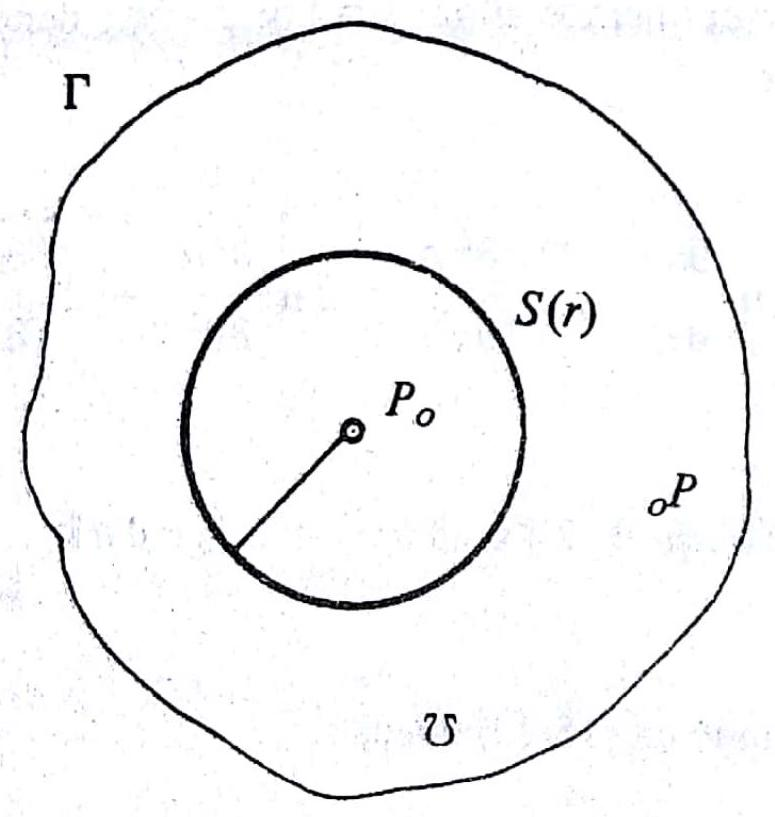
\includegraphics[width=\textwidth]{2025_09_05_adecef5eb2053bc129b5g-363}
\captionsetup{labelformat=empty}
\caption{Figura 17}
\end{center}
\end{figure}

$$
\begin{gathered}
\iint_{\Gamma}\left\{\left\|P-P_{0}\right\|^{-1} \frac{\partial u}{\partial \eta_{c}}-u \frac{\partial}{\partial \eta_{e}}\left\|P-P_{0}\right\|^{-1}\right\} d \sigma= \\
=\iint_{S(r)} \frac{1}{r} \frac{\partial u}{\partial \eta_{e}} d \sigma+\iint_{S(r)} \frac{1}{r^{2}} u d \sigma
\end{gathered}
$$

Pero la primera integral del segundo miembro, por (15-22) vale cero. Aplicando el teorema del valor medio, la segunda integral resulta

$$
\frac{1}{r^{2}} \iint_{S(r)} u d \sigma=\frac{1}{r^{2}} 4 \pi r^{2} u(Q)
$$

donde $Q$ es un punto de $S(r)$. Como para $r \rightarrow 0, \quad u(Q) \rightarrow u\left(P_{0}\right)$ podemos finalmente escribir la fórmula


\begin{equation*}
u\left(P_{0}\right)=\frac{1}{4 \pi} \iint_{\Gamma}\left\{\left\|P-P_{0}\right\|^{-1} \frac{\partial u}{\partial \eta_{e}}-u \frac{\partial}{\partial \eta_{e}}\left\|P-P_{c}\right\|^{-1}\right\} d \sigma \tag{$15\cdot-24$}
\end{equation*}


que nos da los valores de una función armónica en el interior de un da minio, en función de los valores que toman la función y su derivada en la frontera.

Apliquemos ahora (15-24) al caso en que $\Omega$ sea una bola de centro $P_{0}$ y radior. Resulta:

$$
u\left(P_{0}\right)=\frac{1}{4 \pi}\left(\frac{1}{r} \iint_{\Gamma} \frac{\partial u}{\partial \eta_{c}}+\frac{1}{r^{2}} \iint_{\Gamma} u d \sigma\right)
$$

Teniendo en cuenta (15-22) obtenemos la fórmula de la media para las funciones armónicas:

$$
u\left(P_{0}\right)=\frac{1}{4 \pi r^{2}} \iint_{1} u d \sigma
$$

En el caso de la ecuación de Laplace, el problema que interesa resolver es el de Dirichlet. De acuerdo con lo dicho, este problema se enuncia así:

Dado un volumen $\Omega$ en el espacio $R^{n}$ y una función $f(P)$ definida sobre la frontera $\Gamma$ de $\Omega$, se trata de encontrar una función $u$ armónica en $\Omega$ y que coincida con $f$ en $\Gamma$.

Admitiremos la existencia de una solución de este problema y demostraremos la unicidad.

Esto es equivalente a decir que si $u$ es armónica en $\Omega$ y nula es $\Gamma$ es nula en todo $\Omega$. Ahora bien, la fórmula (15-23) nos dice que


\begin{equation*}
\iiint_{\Omega 2}\|\operatorname{grad} u\|^{2} d x d y d z=\iint_{\Gamma} u \frac{\partial u}{\partial \eta_{c}}=0 \tag{15-25}
\end{equation*}


Luego en $\Omega$ es $\|\operatorname{grad} u\|=0$, lo que implica que $u$ es constante en $\Omega y$ como esta función es nula en $\Gamma$, debe ser $u=0$.

Una variante del problema de Dirichlet es el denominado problema de Neumann.

Con las hipótesis anteriores se trata de encontrar una función $u$ armónica en $\Omega$ y tal que $\delta u / \delta \eta_{e}$ coincida con $f^{\prime}$ en $\Gamma$.


En virtud de (15-22), $f$ debe ser tal que

$$
\int j_{\Gamma} f d \sigma=0 .
$$

Vamos a demostrar que esta condición es también suficiente.\\
La fórmula (15-25) nos dice que

$$
\frac{\partial \mu}{\partial \eta_{e}}=0 \text { en } \Gamma \Rightarrow\|\operatorname{grad} u\|=0 \text { en } \Omega \Rightarrow u \text { es constante en } \Omega .
$$

Luego, salvo por adición de una constante, la solución del problema de Neumann es única; es decir, que si $u_{1}$ y $u_{2}$ son soluciones, se tiene $u_{1}-u_{2}=$ constante en $\Omega$.

Vamos ahora a resolver por separación de variables algunos problemas de Dirichlet, asociados a la ecuación de Laplace.

\section*{PROBLFMA DE DIRICHLET PARA EL RECTANGULO}
Sea $R$ el rectángulo $[0, a] \times[0, b]$ en $R^{2}$. Vamos a encontrar una función $u(x, y)$ que sea armónica en el interior de $R$ y tal que sobre el contorno del rectángulo se tenga

\[
\begin{array}{ll}
u(x, 0)=0 ; u(x, b)=f(x) & \text { para } 0 \leqslant x \leqslant a ; \\
u(0, y)=u\left(a, y^{\prime}\right)=0 & \text { para } 0 \leqslant y \leqslant b . \tag{15-26}
\end{array}
\]

Busquemos una solución de la forma $X(x) . Y(y)$\\
Reemplazando en (15-19) es

$$
X^{\prime \prime} \cdot Y+X \cdot Y^{\prime \prime}=0
$$

Luego, debe existir una constante $\lambda$, tal que

$$
\frac{X^{\prime \prime}}{X}=-\frac{Y^{\prime \prime}}{Y}=\lambda
$$

0 equivalent emente

$$
\left\{\begin{array}{l}
X^{\prime \prime}-\lambda X=0 \\
Y^{\prime \prime}+\lambda Y=0
\end{array}\right.
$$

De (15-26) resulta $X(0)=X(a)=0$; luego $X$ debe satisfacer un problema de Sturm-Liouville ya conocido,

$$
X^{\prime \prime}-\lambda X=0 \quad, \quad X(0)=X(a)=0
$$

cuyos autovalores y autovectores son, respectivamente:

$$
\begin{aligned}
\lambda_{n} & =-\left(\frac{n \pi}{a}\right)^{2} \\
X_{n}(x) & =\operatorname{sen} \frac{n \pi}{a} x
\end{aligned} \quad \text { para } n=1,2, \ldots
$$

En cuanto a la ecuación para $Y$, reemplazando $\lambda$ por $\lambda_{n}$, su integral general es

$$
Y_{n}(y)=A_{n} \operatorname{sh} \frac{n \pi}{a} y+B_{n} \operatorname{ch} \frac{n \pi}{a} y .
$$

La condición (15-26) implica $Y_{n}(0)=0$, luego $B_{n}=0$.\\
Superponiendo soluciones obtenemos la función


\begin{equation*}
u(x, y)=\sum_{n=1}^{\infty}\left(A_{n} \operatorname{sh} \frac{n \pi}{a} y\right) \quad \operatorname{sen} \frac{n \pi}{a} x . \tag{15-27}
\end{equation*}


Para que cumpla las condiciones (15-26) impuestas, debe ser

$$
f(x)=u(x, b)=\sum_{n=1}^{\infty}\left(A_{n} \operatorname{sh} \frac{n \pi}{a} b\right) \operatorname{sen} \frac{n \pi}{a} x .
$$

Es decir,

$$
A_{n} \operatorname{sh} \frac{n \pi}{a} b
$$

es el enésimo coeficiente del desarrollo en serie de senos de $f(x)$ en $[0, a]$.\\
Por lo tanto, la solución del problema de Dirichlet planteado es la función (15-27) con

$$
A_{n}=\frac{2}{a \operatorname{sh} \frac{n \pi b}{a}} \int_{0}^{n} f(x) \operatorname{sen} n \frac{\pi}{a} x d x
$$

\section*{PROBLEMA DE DIRICHLET PARA EL PARALELEPIPEDO}
Sea $P$ el paralelepípedo $[0, a] \times[0, b] \times[0, c]$ en $R^{3}$. Se pide determinar una función armónica en el interior de $P$ y tal que sobre la frontera $\operatorname{de} P$ se tenga

\[
\begin{array}{ll}
u(0, y, z)=0 & \\
u(a, y, z)=0 & 0 \leqslant y \leqslant b ; 0 \leqslant z \leqslant c \\
u(x, 0, z)=0 & \\
u(x, b, z)=0 & 0 \leqslant x \leqslant a ; 0 \leqslant z \leqslant c \\
u(x, y, 0)=0 & \\
u(x, y, c)=f(x, y) & 0 \leqslant x \leqslant a ; 0 \leqslant y \leqslant b \tag{15-29}
\end{array}
\]

Vamos a aplicar el método de separación de variables.\\
Busquemos una solución de la forma

$$
u(x, y, z)=X(x) Y(y) Z(z)
$$

puesto que $u$ ha de ser una función armónica, debe cumplir:

$$
X^{\prime \prime} Y Z+X Y^{\prime \prime} Z+Z Y Z^{\prime \prime}=0
$$

Dividiendo por $u$ queda

$$
\frac{X^{\prime \prime}}{X}+\frac{Y^{\prime \prime}}{Y}+\frac{Z^{\prime \prime}}{Z}=0
$$

Por lo tanto cualesquiera que sean $\alpha$ y $\beta$, si $X, Y, Z$ son soluciones de las ecuaciones

$$
X^{\prime \prime}-\alpha X=0 ; Y^{\prime \prime}-\beta Y=0 ; Z^{\prime \prime}+(\alpha+\beta) Z=0
$$

la función $u=X . Y . Z$ será armónica en $P$.\\
De (15-29) resulta:

$$
\begin{aligned}
& X(0)=X(a)=0 \\
& Y(0)=Y(b)=0
\end{aligned}
$$

Luego $X$ e $Y$ deben ser soluciones del mismo problema de SturnLiouville que en el caso del rectángulo.

Es entonces

$$
\begin{array}{ll}
\alpha_{n}=-\left(\frac{n \pi}{a}\right)^{2}: X_{n}(x)=\operatorname{sen} \frac{n \pi}{a} x \quad \text { para } n=1,2, \ldots: \\
\beta_{m}=-\left(\frac{m \pi}{b}\right)^{2}: Y_{m}(y)=\operatorname{sen} \frac{m \pi}{h}, \quad \text { para } m=1,2 \ldots .
\end{array}
$$

Reemplazando $\alpha_{n}$ y $\beta_{m}$ en la ecuación diferencial que debe cumplir $Z$. se tiene como solución:


$$
Z_{m}^{n}(z)=A_{m}^{n} \operatorname{sh}\left[\pi\left(\frac{n^{2}}{a^{2}}+\frac{m^{2}}{b^{2}}\right)^{1 / 2} z\right]+B_{m}^{n} \operatorname{ch}\left[\pi\left(\frac{n^{2}}{a^{2}}+\frac{m^{2}}{b^{2}}\right)^{1 / 2} z\right]
$$

$$
\text { Como } Z_{m}^{n}(0)=0 \text { se tiene } B_{m}^{n}=0 .
$$

Superponiendo soluciones obtenemos


\begin{gather*}
u(x, y, z)= \\
=\sum_{m, n=1}^{\infty}\left\{A_{m}^{n} \operatorname{sh}\left[\pi\left(\frac{n^{2}}{a^{2}}+\frac{m^{2}}{b^{2}}\right)^{1 / 2} z\right] \operatorname{sen} \frac{n \pi}{a} x \operatorname{sen} \frac{m \pi}{b}\right\} \tag{15-30}
\end{gather*}


Aplicando ahora las condiciones que figuran en (15-29) sobre la variable $z$, resulta


\begin{gather*}
f(x, y)=u(x, y, c)= \\
=\sum_{m, n=1}^{\infty}\left\{A_{m}^{n} \operatorname{sh}\left[\pi\left(\frac{n^{2}}{a^{2}}+\frac{m^{2}}{b^{2}}\right)^{1 / 2} c\right] \operatorname{sen} \frac{n \pi}{a} x \operatorname{sen} \frac{m \pi}{b} x .\right\} \tag{15-31}
\end{gather*}


Esto significa que

$$
A_{m}^{n} \operatorname{sh}\left[\pi\left(\frac{n^{2}}{a^{2}}+\frac{m^{2}}{b^{2}}\right)^{1 / 2} c\right]
$$

es el ( $\mathrm{m}, \mathrm{n}$ )ésimo coeficiente del desarrollo de la función $f(x, y)$ en serie doble de senos en el rectángulo $[0, a] \times[0, b]$.*

Entonces la solución del problema de Dirichlet planteado es la función (15-30), con

$$
A_{m}^{n}=\frac{2}{a \cdot b \cdot \operatorname{sh}\left[\pi\left(\frac{n^{2}}{a^{2}}+\frac{m^{2}}{b^{2}}\right)^{1 / 2} c\right]} \int_{0}^{a} \int_{0}^{b} f(x, y) \operatorname{sen} \frac{n \pi}{a} x \operatorname{sen} \frac{n \pi}{b} y d x d y^{*}
$$

\begin{itemize}
  \item Admitiremos esta fórmula, generalización de la del desarrollo en serie simple de senos.
\end{itemize}

ECUACION DE LAPLACE EN COORDENADAS CURVILINEAS\\
En los problemas de teoría del potencial sobre cilindros, conos o esferas, es preferible utilizar coordenadas curvilíneas.

La expresión del laplaciano en coordenadas cilíndricas y esféricas es respectivamente:


\begin{gather*}
\Delta(r, \varphi, z)=\frac{1}{r}\left[\frac{\partial}{\partial r}\left(r \frac{\partial u}{\partial r}\right)+\frac{1}{r} \frac{\partial^{2} u}{\partial \varphi^{2}}\right]+\frac{\partial^{2} u}{\partial z^{2}}  \tag{15-32}\\
\Delta(r, \varphi, \theta)=\frac{1}{r^{2}}\left[\frac{\partial}{\partial r}\left(r^{2} \frac{\partial u}{\partial r}\right)+\frac{1}{\operatorname{sen} \theta} \frac{\partial}{\partial \theta}\left(\operatorname{sen} \theta \frac{\partial u}{\partial \theta}\right)+\frac{1}{\operatorname{sen}^{2} \varphi} \frac{\partial^{2} u}{\partial \varphi^{2}}\right] . \tag{15-33}
\end{gather*}


Si en (15-32) suponemos que $u$ no depende de $z$, obtendremos la fórmula del laplaciano en coordenadas polares. Vamos a estudiar el problema de Dirichlet en este caso.

Se trata entonces del estudio del problema de Dirichlet asociado a la ecuación

$$
\frac{1}{r}\left[\frac{\partial}{\partial r}\left(r \frac{\partial u}{\partial r}\right)+\frac{1}{r} \frac{\partial^{2} u}{\partial \varphi^{2}}\right]=0
$$

o lo que es lo mismo, multiplicando por $r^{2}$ :


\begin{equation*}
r^{2} \frac{\partial^{2} u}{\partial r^{2}}+r \frac{\partial u}{\partial r}=-\frac{\partial^{2} u}{\partial \varphi^{2}} \tag{15-34}
\end{equation*}


Apliquemos el método de separación de variables a (15-34).\\
Sea $u(r, \varphi)=R(r) \Phi(\varphi)$.\\
Para que $u$ verifique (15-34) se deberá cumplir

$$
r^{2} \Phi R^{\prime \prime}+r \Phi R^{\prime}=-R \Phi^{\prime \prime}
$$

$\mathrm{E}_{S}$ decir, existe una constante $\lambda$ tal que


$$
\frac{r^{2} R^{\prime \prime}+r R^{\prime}}{R}=-\frac{\Phi^{\prime \prime}}{\Phi}=\lambda .
$$

Luego $\Phi$ tiene que ser solución de la ecuación $\Phi^{\prime \prime}+\lambda \Phi=0$.\\
Pero como $\varphi$ es un ángulo, las soluciones de esta ecuación deberán ser funciones de período $2 \pi$. Por lo tanto queda planteado un problema de Sturm-Liouville con condiciones de periodicidad en los límites:

$$
\Phi(-\pi)=\Phi(\pi) \quad ; \quad \Phi^{\prime}(-\pi)=\Phi^{\prime}(\pi) .
$$

Ya vimos que los autovalores y autovectores eran

$$
\begin{aligned}
\lambda_{n} & =n^{2} & & \text { para } n=0,1,2, \ldots ; \\
\Phi_{0}(\varphi) & =1 & & \\
\Phi_{n}(\varphi) & =\operatorname{sen} n \varphi, \cos n \varphi & & \text { para } n=1,2, \ldots
\end{aligned}
$$

Para $n=0$, la ecuación en $r$ es

$$
r^{2} R^{\prime \prime}+r R^{\prime}=0 .
$$

Su integral general resulta ser

$$
R(r)=a_{u}+b_{0} \log r .
$$

Para $n>0$, la ecuación en $r$ es, en cambio,

$$
r^{2} R^{\prime \prime}+r R^{\prime}-n^{2} R=0 .
$$

0 sea, es una ecuación de Euler, con integral general

$$
R(r)=C_{n}^{1} r^{n}+C_{n}^{2} r^{n} .
$$

Por to tanto siempre que se cumplan las condiciones necesarias de\\
convergencia, toda función de la forma


\begin{align*}
u(r, \varphi)= & a_{0}+b_{0} \log r+\sum_{n=1}^{\infty}\left(a_{n} \cos n \varphi+b_{n} \operatorname{sen} n \varphi\right) r^{n}+ \\
& +\sum_{n=1}^{\infty}\left(A_{n} \cos n \varphi+B_{n} \operatorname{sen} n \varphi\right) r^{-n} \tag{15-35}
\end{align*}


es solución de (15-34).\\
Vamos ahora a imponer tres tipos distintos de condiciones sobre la función, dando origen así a tres problemas de Dirichlet diferentes.\\
I) $u(r, \varphi)$ debe ser solución de (15-34) en el disco $r<R$ y además tiene que cumplir $u(r, \varphi)=f(\varphi)$.

Puesto que para $r \rightarrow 0$ los términos donde figuran $\log r$ y $r^{-n}$ no están acotados, debe ser

$$
b_{0}=A_{n}=B_{n}=0 \quad \text { para } n=1,2, \ldots
$$

Entonces (15-35) se reduce a


\begin{equation*}
u(r, \varphi)=a_{0}+\sum_{n=1}^{\infty}\left(a_{n} \cos n \varphi+b_{n} \operatorname{sen} n \varphi\right) r^{n} \tag{15-36}
\end{equation*}


Debe cumplirse

$$
f(\varphi)=u(R, \varphi)=a_{0}+\sum_{n=1}^{\infty}\left(a_{n} \cos n \varphi+b_{n} \operatorname{sen} n \varphi\right) R^{n}
$$

Los coeficientes son entonces los del desarrollo en serie de Fourier de $f$. Por lo tanto la solución del problema viene dada por la función (15-36) con

$$
a_{0}=\frac{1}{2 \pi} \int_{-\pi}^{\pi} f(\varphi) d \varphi ;
$$


$$
\begin{aligned}
& a_{n}=\frac{1}{\pi R^{n}} \int_{-\pi}^{\pi} f(\varphi) \cos n \varphi d \varphi \quad \text { para } n=1,2, \ldots, \\
& b_{n}=\frac{1}{\pi R^{n}} \int_{-\pi}^{\pi} f(\varphi) \operatorname{sen} n \varphi d \varphi .
\end{aligned}
$$

II) $u(r, \varphi)$ debe ser solución de (15-34) en el exterior de un disco de radio $R$, cumpliendo

$$
\begin{aligned}
& \lim _{r \rightarrow \infty} u(r, \varphi)=0 \\
& u(R, \varphi)=f(\varphi)
\end{aligned}
$$

A $f$ le imponemos además la condición

$$
\int_{-\pi}^{\pi} f(\varphi) d \varphi=0
$$

La condición de anulación en el infinito nos sugiere tomar en (15-35) $a_{0}=b_{0}=a_{n}=b_{n}=0$.

La solución será entonces de la forma


\begin{equation*}
u(r, \varphi)=\sum_{n=1}^{\infty}\left(A_{n} \cos n \varphi+B_{n} \operatorname{sen} n \varphi\right) r^{-n} \tag{15-37}
\end{equation*}


Debe cumplirse

$$
f(\varphi)=\sum_{n=1}^{\infty}\left(A_{n} \cos n \varphi+B_{n} \operatorname{sen} n \varphi\right) R^{-n}
$$

Entonces (15-37) es la solución del problema planteado, con

$$
A_{n}=\frac{R^{n}}{\pi} \int_{-\pi}^{\pi} f(\varphi) \cos n \varphi d \varphi ; B_{n}=\frac{R^{n}}{\pi} \int_{-\pi}^{\pi} f(\varphi) \operatorname{sen} n \varphi d \varphi
$$

III) $u(r, \varphi)$ debe ser solución de (15-34) en la corona $R_{1} \leqslant r \leqslant R_{2} y^{\text {se }}$ deben cumplir las condiciones

$$
u\left(R_{1}, \varphi\right)=f_{1}(\varphi) \quad, \quad u\left(R_{2}, \varphi\right)=f_{2}(\varphi), \quad-\pi \leqslant \varphi \leqslant \pi
$$

En este caso será necesario usar todos los términos de (15-35), y los coeficientes deberán cumplir las condiciones:

$$
\begin{aligned}
f_{1}(\varphi) & =a_{0}+b_{0} \log R_{1}+ \\
& +\sum_{n=1}^{\infty}\left[\left(R_{1}^{n} a_{n}+R_{1}^{-n} A_{n}\right) \cos n \varphi+\left(R_{1}^{n} b_{n}+R_{1}^{-n} B_{n}\right) \operatorname{sen} n \varphi\right]
\end{aligned}
$$

$$
\begin{aligned}
f_{2}(\varphi) & =a_{0}+b_{0} \log R_{2}+ \\
& +\sum_{n=1}^{\infty}\left[\left(R_{2}^{n} a_{n}+R_{2}^{-n} A_{n}\right) \cos n \varphi+\left(R_{2}^{n} b_{n}+R_{2}^{n} B_{n}\right) \cos n \varphi\right] .
\end{aligned}
$$

Obtenemos así dos desarrollos en serie de Fourier, de los cuales resulta


\begin{align*}
& \left\{\begin{array}{l}
a_{0}+b_{0} \log R_{1}=\frac{1}{2 \pi} \int_{-\pi}^{\pi} f_{1}(\varphi) d \varphi \\
a_{0}+b_{0} \log R_{2}=\frac{1}{2 \pi} \int_{-\pi}^{\pi} f_{2}(\varphi) d \varphi
\end{array}\right.  \tag{15-38}\\
& \left\{\begin{array}{l}
a_{n} R_{1}^{n}+A_{n} R_{1}^{-n}=\frac{1}{\pi} \int_{-\pi}^{\pi} f_{1}(\varphi) \cos n \varphi d \varphi \\
a_{i n} R_{2}^{n}+A_{n} R_{2}^{-n}=\frac{1}{\pi} \int_{-\pi}^{\pi} f_{2}(\varphi) \cos n \varphi d \varphi
\end{array}\right. \tag{15-39}
\end{align*}



\[
\left\{\begin{array}{l}
\quad \quad \text { para } n=1,2, \ldots \\
b_{n} R_{1}^{n}+B_{n} R_{1}^{-n}=\frac{1}{\pi} \int_{-\pi}^{\pi} f_{1}(\varphi) \operatorname{sen} n \varphi d \varphi  \tag{15-40}\\
b_{n} R_{2}^{n}+B_{n} R_{2}^{-n}=\frac{1}{\pi} \int_{-\pi}^{\pi} f_{2}(\varphi) \operatorname{sen} n \varphi d \varphi
\end{array}\right.
\]

En cada uno de los sistemas, el determinante de los coeficientes es no nulo; luego estos sistemas son siempre resolubles. Por lo tanto la solución del problema es la función (15-35) cuando los coeficientes son las soluciones de los sistemas (15-38), (15-39) y (15-40).

Volvamos ahora a la ecuación (15-32) y supongamos que $u$ no depende de $\varphi, 0$ lo que es lo mismo, que el potencial se toma con simetría radial; la ecuación (15-31) es entonces de la forma

$$
\frac{1}{r}\left[\frac{\partial}{\partial r}\left(r \frac{\partial u}{\partial r}\right)\right]+\frac{\partial^{2} u}{\partial z^{2}}=0
$$

o equivalentemente,


\begin{equation*}
\frac{\partial^{2} u}{\partial r^{2}}+\frac{1}{r} \frac{\partial u}{\partial r}+\frac{\partial^{2} u}{\partial z^{2}}=0 . \tag{15-41}
\end{equation*}


El problema de Dirichlet que vamos a estudiar es el siguiente:\\
Encontrar una función $u(z, r)$ que sea solución de (15-41) en $z>0$, $0 \leqslant r<a$ y que cumpla además las condiciones


\begin{equation*}
\lim _{z \rightarrow \infty} u(z, r)=0 \quad ; \quad u(z, a)=0 \quad ; \quad u(0, r)=f(r) . \tag{15-42}
\end{equation*}


Aplicando el método de separación de variables, hay que buscar una solución de (15-41) de la forma $u(z, r)=Z(z) R(r)$.

Se tiene

$$
\left(R^{\prime \prime}+\frac{1}{r} R^{\prime}\right) Z=-Z^{\prime \prime} R .
$$

Luego es

$$
\frac{R^{\prime \prime}+\frac{1}{r} R^{\prime}}{-R}=\frac{Z^{\prime \prime}}{Z}=\lambda .
$$

Si ponemos $\lambda=k^{2}$, la ecuación en $R$ es la de Bessel

$$
R^{\prime \prime}+\frac{1}{r} R^{\prime}+k^{2} R=0,
$$

que tiene como solución acotada en $r=0$ a $J_{0}(k r)$.\\
La segunda de las condiciones (15-42) implica que debe ser $J_{0}(k a)=0$.

Por lo tanto, los valores de $\lambda$ que hay que tomar son

$$
\lambda=\lambda_{n}=\left(\frac{\alpha_{n}}{a}\right)^{2}
$$

donde $\left\{\alpha_{n}\right\}$ es la sucesión de las raíces positivas de $J_{0}(r)$.\\
La ecuación en $A$ es de la forma $Z$ " $-\lambda_{n}^{2} Z=0$, cuya integral general es

$$
Z(z)=A_{n} e^{-a_{n} z}+B_{n} e^{a_{n} z} .
$$

Como $\alpha_{n}>0$, la primera de las condiciones (15-42) implica $B_{n}=0$. Superponiendo las soluciones, se obtiene la función


\begin{equation*}
u(z, r)=\sum_{n=1}^{\infty} A_{n} J_{0}\left(\alpha_{n} r\right) e^{-a_{n} z}, \tag{15-43}
\end{equation*}


que cumple las dos primeras condiciones de (15-42). Cumplirá la tercera si

$$
f(r)=u(0, r)=\sum_{n=1}^{\infty} A_{n} J_{0}\left(\alpha_{n} r\right),
$$

es decir, si $A_{n}$ es el enésimo coeficiente de Fourier-Bessel de $f$.\\
Luego la solucióni del problema es la función (15-43), cuando los coeficientes $A_{n}$ vienen dados por

$$
A_{n}=\frac{2}{a^{2}\left[J_{0}^{\prime}\left(\alpha_{n} a\right)\right]^{2}} \int_{0}^{a} r f(r) J_{0}\left(\alpha_{n} r\right) d r .
$$

Consideremos ahora el caso de un potencial en coordenadas esféricas con simetría radial; es decir, independiente de $\varphi$.

La ecuación (15-33), después de multiplicar por $r^{2}$ toma la forma


\begin{equation*}
r^{2} \frac{\partial^{2} u}{\partial r^{2}}+2 r \frac{\partial u}{\partial r}+\frac{\partial^{2} u}{\partial \theta^{2}}+\operatorname{ctg} \theta \frac{\partial u}{\partial \theta}=0 . \tag{15-44}
\end{equation*}


Vamos a resolver esta ecuación por el metodo de separación de variables. Busquemos una solución de la forma $u(r, \theta)=R(r) T(\theta)$.

Se debe cumplir

$$
T\left[r^{2} R^{\prime \prime}+2 r R^{\prime}\right]=-R\left[T^{\prime \prime}+\operatorname{ctg} \theta T^{\prime}\right] .
$$

Cualquiera que sea $\lambda, u(r, \theta)$ será solución de la ecuación (15-44) si $T$ y $R$ son soluciones de

$$
"+\operatorname{ctg} \theta T^{\prime}+\lambda T=0 ; r^{2} R^{\prime \prime}+2 r R^{\prime}-\lambda R=0 .
$$

en 0 yen $\pi$.

La función $u$ es solución para $0 \leqslant \theta \leqslant \pi$; luego $T$ debe ser acotada

La ecuación diferencial en $T$ es por lo tanto, la ecuación de Legendre en forma angular.

La solución debe ser acotada en $\pm 1=\cos \theta$. Luego se debe tener

$$
\begin{array}{rlr}
\alpha_{n} & =n(n+1), & \\
T_{n}(\theta) & =P_{n}(\cos \theta), & \text { para } n=0,1,2, \ldots
\end{array}
$$

La ecuación en $R$ es ahora $r^{2} R^{\prime \prime}+2 r R^{\prime}-n(n+1) R=0$, que es una ecuación de Euler. Su infegral general es

$$
R_{n}=C_{n}^{1} r^{n}+\frac{C_{n}^{2}}{r^{n+1}} .
$$

Por lo tanto, siempre que se cumplan las condiciones de convergencia de la serie, la función


\begin{equation*}
u(r, \theta)=\sum_{n=0}^{\infty}\left(a_{n} r^{n}+B_{n} \frac{1}{r^{n+1}}\right) P_{n}(\cos \theta) \tag{15-45}
\end{equation*}


es una solución de la ecuación (15-44).

Apliquemos esto para resolver el siguiente problema de Dirichlet: $u(r, \theta)$ debe ser solución de (15-44) en la esfera $r<R$ y se debe tener sobre la superficie esférica

$$
u(R, \theta)=f(\theta)
$$

Como debe ser solución para $r=0$ tendremos que tomar $B_{n}=0$, para todo $n$. Entonces la solución es de la forma

$$
u(r, \theta)=\sum_{0}^{\infty} A_{n} r^{n} P_{n}(\cos \theta)
$$

Como tiene que cumplirse


$$
f(\theta)=u(R, \theta)=\sum_{0}^{\infty} A_{n} R^{n} P_{n}(\cos \theta) .
$$

$A_{n} R^{n}$ es el enésimo coeficiente del desarrollo en serie de Fourier. Legendre de $f$. La solución es pues la (15-46) con

$$
A_{n}=\frac{2 n+1}{2 R^{n}} \int_{0}^{\pi} f(\theta) P_{n}(\cos \theta) \operatorname{sen} \theta d \theta
$$

Se puede considerar también el siguiente problema de Dirichlet: $u(r ; \theta)$ debe ser solución de (15-44) en el exterior de una esfera de radio $R$, y cumplir las condiciones

$$
\lim _{r \rightarrow \infty}(r, \theta)=0 \quad, \quad u(R, \theta)=f(\theta)
$$

La primera de estas condiciones nos dice que en (15-45) los coeficientes $a_{n}$ : deben ser nulos. Entonces la solución es una función de la forma

$$
u(r, \theta)=\sum_{0}^{\infty} B_{n} \frac{P_{n}(\cos \theta)}{r^{n+1}} .
$$

Por un razonamiento análogo al del problema anterior, resulta

$$
B_{n}=\frac{(2 n+1) R^{n+1}}{2} \int_{0}^{\pi} f(\theta) P_{n}(\cos \theta) \operatorname{sen} \theta d \theta
$$

\section*{PROBLEMA DE CAUCHY PARA LAS ECUACIONES DE LAS ONDAS Y DE LA DIFUSION: CASO DE LAS MEMBRANAS VIBRANTES}
En lo que sigue, los datos entre paréntesis indican las modificaciones que hay que hacer para pasar de la ecuación de las ondas a la de la difusión.

Consideremos la ecuación de las ondas (resp. de la difusión)

$$
\frac{\partial^{2} v}{\partial x_{1}^{2}}+\cdots+\frac{\partial^{2} v}{\partial x_{n}^{2}}=\frac{1}{c^{2}} \frac{\partial^{2} v}{\partial t^{2}} ; \quad\left(\text { resp. } \frac{1}{c^{2}} \frac{\partial v}{\partial t}\right),(15.46)
$$

y el siguiente problema de Cauchy:\\
$\Omega$ es un volumen de $R^{n}$, y $S$ su frontera. Se pide determinar $v$ de forma que\\
a) sea solución de (15-46) para $x=\left(x_{1} \ldots x_{n}\right) \in \Omega$ y para todo $t$ (resp. para todo $t>0$ );\\
b) se anule para $x \in S$;\\
c) cumpla las condiciones iniciales, (resp. sólo la primera)

$$
v(x, 0)=f(x) \quad ; \quad \frac{\partial v}{\partial t}(x, 0) \quad g(x) .
$$

Si tratamos de resolver este problema buscando una solución de la forma $v(x, t)=u(x) T(t)$ se tiene que cumplir

$$
\frac{\Delta u}{u}=\frac{1}{C^{2}} \frac{T^{\prime \prime}}{T} ; \quad\left(\text { resp. } \frac{\Delta u}{u}=\frac{1}{C^{2}} \frac{T^{\prime}}{T}\right)
$$

0 lo que es equivalente, para algún valor de $\lambda$, debe tenerse


\begin{align*}
& \left\{\begin{array}{l}
\Delta u-\lambda u=0 \\
u(x)=0 \quad \text { para } \quad x \in S .
\end{array}\right.  \tag{15-47}\\
& T^{\prime \prime}-\lambda c^{2} T=0 \quad\left(\text { resp. } T^{\prime}-\lambda c^{2} T=0\right)
\end{align*}


Observemos que la condición (15-47) indica que $u$ debe ser solución de un problema de Sturm-Liouville en varias variables.

Vamos a resolver algunos problemas para $n=2$ : en el caso de la ecuación de las ondas, esto corresponde a las membranas vibrantes.


\section*{I) Membrana cuadrada}
Aquí es $\Omega=[0, \pi] \times[0, \pi]$ y las condiciones iniciales tienen la forma

$$
v(x, y, 0)=f(x, y) \quad, \frac{\partial}{\partial t} v(x, y, 0)=g(x, y) .
$$

Entonces (15-47) se escribe

\[
\begin{array}{ll}
\frac{\partial^{2} u}{\partial x^{2}}+\frac{\partial^{2} u}{\partial y^{2}}=\lambda u & \\
u(x, 0)=u(x, \pi)=0 & \text { para } 0 \leqslant x \leqslant \pi \\
u(0, y)=u(\pi, y)=0 & \text { para } 0 \leqslant y \leqslant \pi \tag{15-48}
\end{array}
\]

Resolvamos este problema mediante separación de variables. Busquemos una solución de la forma $u(x, y)=X(x) . Y(y)$.

Se tiene

$$
X^{\prime \prime} Y+Y^{\prime \prime} X=\lambda X Y,
$$

o bien, dividiendo por $u$ :

$$
\lambda=\frac{X^{\prime \prime}}{X}+\frac{Y^{\prime \prime}}{Y} .
$$

Por lo tanto, si $X$ e $Y$ son soluciones de las ecuaciones diferenciales

$$
X^{\prime \prime}-\alpha X=0 \quad ; \quad Y^{\prime \prime}-\beta Y=0
$$

y si suponemos $\lambda=\alpha+\beta$, tendremos una solución de la ecuación.\\
Pero las condiciones en la frontera de (15-48), nos dan como condiciones para $X$ e $Y$

$$
X(0)=X(\pi)=0 \quad ; \quad Y(0)=Y(\pi)=0
$$

Es decir, se obtienen problemas de Sturm-Liouville para $X$ y para $Y$.\\
Los autovalores y autovectores serán

$$
\alpha_{n}=-n^{2} ; \beta_{m}=-m^{2} ; X_{n}(x)=\operatorname{sen} n x ; Y_{m}(y)=\operatorname{sen} m y
$$

para $n, m=1,2, \ldots$\\
La ecuación en $T$ resulta:


\begin{equation*}
T^{\prime \prime}+c^{2}\left(m^{2}+n^{2}\right) T=0 \tag{15-49}
\end{equation*}


Su integral general es

$$
T_{m}^{n}(t)=A_{m}^{n} \operatorname{sen}\left[c\left(m^{2}+n^{2}\right)^{1 / 2} t\right]+B_{m}^{n} \cos \left[c\left(m^{2}+n^{2}\right)^{1 / 2} t\right]
$$

Por lo tanto, siempre con hipótesis de convergencia, la función


\begin{align*}
v(x, y, t) & =\sum_{m, n=1}^{\infty}\left\{A_{n}^{m} \operatorname{sen}\left[c\left(m^{2}+n^{2}\right)^{1 / 2} t\right]+\right. \\
& \left.+B_{m}^{n} \cos \left[c\left(m^{2}+n^{2}\right)^{1 / 2} t\right]\right\} \operatorname{sen} n x \operatorname{sen} m y \tag{15-50}
\end{align*}


cumple las condiciones a) y b).\\
Para que cumpla c) se debe tener

$$
\begin{aligned}
& v(x, y, 0)=f(x, y)=\sum_{n, m=1}^{\infty} B_{m}^{n} \operatorname{sen} n x \operatorname{sen} m y ; \\
& \frac{\partial y}{\partial t}(x, y, 0)=g(x, y)=\sum_{m, n=1}^{\infty} c\left(n^{2}+m^{2}\right)^{1 / 2} A_{m}^{n} \operatorname{sen} n x \operatorname{sen} m y .
\end{aligned}
$$

\section*{MATEMATICA AVANZADA PAFA LA FISICA}
Los coeficientes se deducen de los desarrollos en series dobles de senos de $f$ y $g$ en $[0 . \pi] \times[0, \pi]$.

Por lo tanto la solución del problema es la función (15-50) con

$$
\begin{aligned}
& B_{n}^{m}=\frac{4}{\pi^{2}} \int_{0}^{\pi} \int_{0}^{\pi} f(x, y) \operatorname{sen} n x \operatorname{sen} m y d x d y \\
& A_{n}^{m}=\frac{4}{\pi^{2} c\left(n^{2}+m^{2}\right)^{1 / 2}} \int_{0}^{\pi} \int_{0}^{\pi} g(x, y) \operatorname{sen} n x \operatorname{sen} m y d x d y
\end{aligned}
$$

Si en lugar de considerar la ecuación de las membranas hubiéramos considerado la ecuación de la difusión, en lugar de la ecuación (15-49) se hubiera tenido

$$
T^{\prime}+\left(n^{2}+m^{2}\right) c^{2} T=0
$$

cuya solución es

$$
T(t)=e^{-c^{2}\left(m^{2}+n^{2}\right) t}
$$

La solución del problema es ahora la función

$$
v(x, y, t)=\sum_{m, n=1}^{\infty} A_{n}^{m} \operatorname{sen}(n x) \cdot \operatorname{sen}(m \cdot) e^{-c^{2}\left(m^{2}+n^{2}\right) t}
$$

con

$$
A_{n}^{m}=\frac{4}{\pi^{2}} \int_{0}^{\pi} \int_{0}^{\pi} f(x, y) \operatorname{sen} n x \operatorname{sen} m y d x d y
$$

II) Membrana circular\\
$\Omega$ es el disco de centro 0 y radio $a$.

Tomando coordenadas polares, la ecuación (15-46) es de la forma

$$
\frac{1}{r}\left[\frac{\partial}{\partial r}\left(r \frac{\partial v}{\partial r}\right)+\frac{1}{r} \frac{\partial^{2} v}{\partial \varphi^{2}}\right]=\frac{1}{c^{2}} \frac{\partial^{2} v}{\partial t^{2}}
$$

Se trata de buscar una función $\nu(r, \varphi, t)$ solución en $\Omega$, con la condición en los límites $\nu(r, \varphi, a)=0$ y las condiciones iniciales

$$
v(r, \varphi, 0)=f(r, \varphi) \quad ; \quad \frac{\partial v}{\partial t}(r, \varphi, 0)=g(r, \varphi)
$$

Como la resolución de este problema es bastante complicada, trataremos el caso más simple en que hay una simetría radial, es decir cuando $u$ no depende de $\varphi$.

Tenemos entonces la ecuación:


\begin{equation*}
\frac{\partial^{2} v}{\partial r^{2}}+\frac{1}{r} \frac{\partial v}{\partial t}=\frac{1}{c^{2}} \frac{\partial^{2} v}{\partial t^{2}} \tag{15-51}
\end{equation*}


Hay que encontrar una solución de la ecuación (15-51) en $r \leqslant a$ y todo $t$, que cumpla\\
a) la condición de los límites: $\quad v(a, t)=0$,\\
b) las condiciones iniciales: $\quad v(r, 0)=f(r) ; \frac{\partial v}{\partial t}(r, 0)=g(r)$.

Apliquemos el método de la separación de variables; sea

$$
v(r, t)=R(r) \cdot T(t)
$$

Se tiene

$$
\frac{R^{\prime \prime}+1 / r R^{\prime}}{R}=\frac{1}{c^{2}} \frac{T^{\prime \prime}}{T}=\lambda
$$

La ecuación $R^{\prime \prime}+1 / r R^{\prime}-\lambda R=0$, es para $\lambda=-k^{2}$, la ecuación de

Bessel de orden cero en la variable $k r$. Su única solución acotada en el origen, salvo multiplicación por constantes, es $J_{0}(k, r)$.

La condición en los límites implica

$$
\lambda_{n}=-\left(\frac{\alpha_{n}}{a}\right)^{2} \quad \text { con } J_{0}\left(\alpha_{n}\right)=0
$$

En cuanto a la ecuación en $T$, su solución es

$$
T(t)=A_{n} \cos \left(\lambda_{n} c t\right)+B_{n} \operatorname{sen}\left(\lambda_{n} c t\right)
$$

Luego una solución de la ecuación que cumple a) es


\begin{equation*}
v(r, t)=\sum_{n=1}^{\infty}\left\{\left[A_{n} \cos \left(\lambda_{n} c t\right)+B_{n} \operatorname{sen}\left(\lambda_{n} c t\right)\right]\right\} J_{0}\left(\alpha_{n} r\right) \tag{15-52}
\end{equation*}


Para que también se cumpla b) debe ser

$$
\begin{aligned}
& f(r)=v(r, 0)=\sum_{n=1}^{\infty} A_{n} J_{0}\left(\alpha_{n} r\right) \\
& g(r)=\frac{\partial v}{\partial t}(r, 0)=\sum_{n=1}^{\infty} B_{n} \lambda_{n} c J_{0}\left(\alpha_{n} r\right)
\end{aligned}
$$

Luego la solución del problema es la función (15-52) con

$$
\begin{aligned}
& A_{n}=\frac{2}{a^{2}\left[J_{0}^{\prime}\left(\alpha_{n} a\right)\right]^{2}} \int_{0}^{a} r f(r) J_{0}\left(\alpha_{n} r\right) d r \\
& B_{n}=\frac{2}{a^{2}\left[J_{0}^{\prime}\left(\alpha_{n} a\right)\right]^{2} \lambda_{n} c} \int_{0}^{a} r g(r) J_{0}\left(\alpha_{n} r\right) d r
\end{aligned}
$$

\section*{Ejercicios}
\begin{enumerate}
  \item Resolver la ecuación diferencial
\end{enumerate}

$$
y^{\prime}=x y\left(1+x^{2}\right)^{-1}\left(1+y^{2}\right) .
$$

Respuesta:

$$
x^{2} y^{2}+x^{2}+k y^{2}+1=0 .
$$

\begin{enumerate}
  \setcounter{enumi}{1}
  \item Resolver la ecuación diferencial
\end{enumerate}

$$
2 x y d x-\left(x^{2}-y^{2}\right) d y=0
$$

y comprobar la solución obtenida.\\
3. Resolver la ecuación diferencial

$$
x\left(3 y^{4}+1\right) d x+\left(6 x^{2} y^{3}-2 y^{2}+7\right) d y=0
$$

y comprobar la solución obtenida.\\
4. Resolver, buscando un factor integrante de la forma $x^{m} y^{n}$, la ecuación diferencial

$$
\left(2 y+3 x^{2} y^{3}\right) d x+\left(3 x+5 x^{3} y^{2}\right) d y=0
$$

\section*{Respuesta:}
$$
x^{-8} y^{-12}-2 x^{-6} y^{-10}=C
$$

\begin{enumerate}
  \setcounter{enumi}{4}
  \item Resolver la ecuación diferencial .
\end{enumerate}

$$
(x-2 y+1) d x+(2 x-y-1) d y^{\prime}=0
$$

haciendo el cambió de variable $x=t+a$ y el de función $z=y+b$. donde $a$ y $b$ son constantes a determinar.

\section*{Respuesta:}
$$
(x+y-2)^{3}=k(x-y)
$$

\begin{enumerate}
  \setcounter{enumi}{5}
  \item Resolver la ecuación diferencial
\end{enumerate}

$$
(6 x y+5 y) d x+\left(3 x^{2}+5 x+3 y^{2}\right) d y=0
$$

y comprobar la solución.\\
7. Resolver la ecuación diferencial

$$
x y^{2} d x+(1-x) d y=0
$$

\section*{Respuesta:}
$$
\log |1-x|+x+y^{-1}=C .
$$

\begin{enumerate}
  \setcounter{enumi}{7}
  \item Resolver las ecuaciones diferenciales
\end{enumerate}

$$
\begin{gathered}
\left(y-x^{2}+x e^{y}\right) y^{\prime}=2 x y-x-e^{y} \\
y^{\prime}-2 x y=e^{x^{2}}
\end{gathered}
$$

y comprobar los resultados.\\
9. Resolver la ecuación diferencial

$$
2 x y y^{\prime}+x^{2}+y^{2}=0
$$

y comprobar la solución obtenida.\\
10. Encontrar la familia de curvas $y=f(x)$, tales que la integral

$$
\int_{0}^{x} f(t) d t
$$

sea igual a la longitud del arco de curva de extremos $[0 f(0)]$ y $[x, f(x)]$; comprobar el resultado.\\
11. Encontrar la familia de trayectorias ortogonales a la familia de curvas $y=a x^{5}$.

\section*{Respuesta:}
$$
x^{2}+5 y^{2}=k^{2}
$$

\begin{enumerate}
  \setcounter{enumi}{11}
  \item Se da la ecuación diferencial $y^{\prime}=x^{2}+y^{2}$; sea $y(x)$ la solución de la ecuación que cumple con la condición $y(0)=1$. Determinar los cinco primeros términos del desarrollo de $y$ en serie de potencias de la variable $x$.
\end{enumerate}

\section*{Respuesta:}
$$
1+x+x^{2}+4 / 3 x^{3}+7 / 6 x^{4}
$$

\begin{enumerate}
  \setcounter{enumi}{12}
  \item Se da la ecuación diferencial $y^{\prime \prime \prime}=x^{2}+y^{2}$; sea $y(x)$ la solución de la ecuación que cumple las condiciones: $y(1)=1, y^{\prime}(1)=0, y^{\prime \prime}(1)=2$. Determinar los cinco primeros términos del desarrollo en serie de potencias de $x-1$ de $y(x)$.
\end{enumerate}

\section*{Respuesta:}
$$
1+(x-1)^{2}+1 / 3(x-1)^{3}+1 / 12(x-1)^{4}+1 / 20(x-1)^{5}
$$

\begin{enumerate}
  \setcounter{enumi}{13}
  \item Resolver la ecuación diferencial
\end{enumerate}

$$
2 y \operatorname{sen} 3 x+3 y^{2} \cos 3 x y^{\prime}=0
$$

Respuesta:

$$
9 y^{2}=4 \log (\cos 3 x)+C
$$

\begin{enumerate}
  \setcounter{enumi}{14}
  \item Encontrar la solución que pasa por el punto $(0,1)$ de la ecuación diferencial
\end{enumerate}

$$
\left(x^{2}+1\right) y^{\prime}+y^{2}+1=0 .
$$

\begin{enumerate}
  \setcounter{enumi}{15}
  \item Resolver la ecuación diferencial
\end{enumerate}

$$
x^{2} y^{\prime}-2 x y=1 / x
$$

y comprobar el resultado.\\
17. Resolver, usando el método del factor integrante, la ecuación diferencial

$$
y e^{x} d x+\left(y-2 e^{x}\right) d y=0
$$

Respuesta:

$$
e^{x}-y-C y^{2}=0 .
$$

\begin{enumerate}
  \setcounter{enumi}{17}
  \item Demostrar que la ecuación diferencial
\end{enumerate}

$$
y(y-x-1) d x+x d y=0
$$

admite un factor integrante de la forma $y^{-2} f(x)$. Resolver la ecuación y comprobar el resultado obtenido.\\
19. Determinar las trayectorias ortogonales a la familia de rectas

$$
y+1=a x .
$$

Respuesta:

$$
(y+1)^{2}+x^{2}=r^{2} .
$$

\begin{enumerate}
  \setcounter{enumi}{19}
  \item Resolver, por separación de variables, la ecuación $y^{\prime}=2 x y$. Comprobar el resultado aplicando el método de desarrollo en serie.
  \item Encontrar la solución de la ecuación diferencial
\end{enumerate}

$$
(x+1) y^{\prime}-(x+2) y=0
$$

que cumple la condición inicial $y(0)=1$ por el desarrollo en serie $y$ por el método de separación de variables.\\
22. Sea $f(z)=u(x, y)+v(x, y) i$ una función holomorfa en un\\
abierto y conexo del plano tal que en él no se anulen simultáneamente las derivadas parciales de las partes real e imaginaria. Probar que las dos familias de curvas $u(x, y)=C, v(x, y)=K$ son ortogonales.\\
23. Resolver las ecuaciones diferenciales que siguen y comprobar en cada caso los resultados obtenidos:

$$
\begin{aligned}
& 2 y^{\prime \prime \prime}-5 y^{\prime \prime}-y^{\prime}+6 y=0 ; \\
& y^{\prime \prime \prime}-3 y^{\prime \prime}+7 y^{\prime}-5 y=0 ; \\
& y^{\prime \prime \prime}-3 y^{\prime \prime}+2 y^{\prime}=0 ; \\
& y^{\prime \prime \prime}+2 y^{\prime \prime}+y=0 .
\end{aligned}
$$

\begin{enumerate}
  \setcounter{enumi}{23}
  \item Determinar la solución de la ecuación diferencial
\end{enumerate}

$$
y^{\prime \prime}-2 y^{\prime}+y=0
$$

que cumple las condiciones $y(0)=1, y^{\prime}(0)=0$. Comprobar el resultado.\\
25. Resolver las ecuaciones diferenciales que siguen y comprobar para cada una de ellas los resultados obtenidos:

$$
\begin{aligned}
& y^{\prime \prime}+y=\operatorname{sen} 3 x \\
& y^{\prime \prime}+5 y^{\prime}+4 y=\cos 2 x \\
& y^{\prime \prime}+4 y^{\prime}+4 y=3 x e^{-2 x} \\
& y^{\prime \prime}+3 y^{\prime}+2 y=6 e^{x} \\
& y^{\prime \prime}-3 y^{\prime}+2 y=\operatorname{sen}\left(e^{-x}\right) \\
& y^{\prime \prime}+4 y=12 \operatorname{sen} 2 x \\
& y^{\prime \prime}-2 y^{\prime}+y=x+e^{x} \\
& \left(y^{\prime \prime}+y\right) \cos x-1=0 \\
& y^{\prime \prime}+4 y^{\prime}+3 y=4 \operatorname{sen} x+8 \cos x
\end{aligned}
$$


$$
\begin{aligned}
& x^{2} y^{\prime \prime}-2 y=\log x \\
& x^{2} y^{\prime \prime}-2 x y^{\prime}+2 y=x^{2}+2 .
\end{aligned}
$$

\begin{enumerate}
  \setcounter{enumi}{25}
  \item Encontrar la solución de la ecuación diferencial
\end{enumerate}

$$
y^{\prime \prime}+y^{\prime} / x+y / x^{2}=0
$$

que cumple las condiciones $y(1)=1, y^{\prime}(1)=0$.\\
27. Resolver las ecuaciones diferenciales siguientes:

$$
\begin{aligned}
& x^{2} y^{\prime \prime}+x y^{\prime}-y=x \\
& x^{2} y^{\prime \prime}+\left(x^{2}+x\right) y^{\prime}-y^{\prime}=0 \\
& \left(1-x^{2}\right) y^{\prime \prime}-2 x y^{\prime}+2 y^{\prime}=0 \\
& x^{2} y^{\prime \prime}-x(x+2) y^{\prime}+(x+2) y^{\prime}=0 \\
& x(x-1) y^{\prime \prime}+\lambda(3 x-1) y^{\prime}+y^{\prime}=0
\end{aligned}
$$

\begin{enumerate}
  \setcounter{enumi}{27}
  \item Demostrar que la llamada ecuaciön hipergeométrica
\end{enumerate}

$$
\left(x-x^{2}\right) y^{\prime \prime}+[c-(a+b+1) x] y^{\prime \prime}-a b_{y}=0
$$

es regular en el sentido de Fuchs.\\
29. Sea la ecuación diferencial . $y^{\prime \prime}+p(x) y^{\prime}+q(x) y^{\prime}=0$, donde se supone que todos los puntos (incluido el del intinito) son puntos de holomorifismo de $p$ y de $q$, con la posible excepción de $n$ puntos en los cuales hay regularidad en el sentido de Fuchs.

Demostrar que para $n=1$ la ecuación puede reducirse a la forma . $\varphi^{\prime \prime}=0$ y que para $n=2$ la ecuación puede reducirse a una ecuación de Fuler.\\
30. Sea la ecuación diererencial

$$
x^{2}(x+1) y^{\prime \prime}+x(a x+4) y^{\prime}+(6 x+2) y=0
$$

Mediante el estudio de las solucionès en un entorno de cero, determinar el valor de $a$ para el cual todas las soluciones de la ecuación sean funciones racionales y calcular para ese valor la integral general.

\section*{Respuesta:}
$$
a=6 \quad Y(x)=A x^{-2}+B\left(x^{3}+x^{2}\right)^{-1}
$$

\begin{enumerate}
  \setcounter{enumi}{30}
  \item Se considera la ecuación diferencial
\end{enumerate}

$$
y^{\prime \prime}+\left(p+1 / 2-x^{2} / 4\right) y=0
$$

donde $p$ es un entero positivo.\\
Demostrar que esta ecuación admite una solución de la forma

$$
H_{p}(x) e^{-x^{2} / 4},
$$

donde $H_{p}$ es un polinomio de grado $p$ y de la paridad de $p$.

\section*{Indicación:}
Se recomienda hacer el cambio de función $y(x)=z(x) e^{-x^{2} / 4}$\\
32. Se considera la ecuación diferencial $x y^{\prime \prime}+2 y^{\prime}+a x y^{\prime}=0$, donde $a$ es un número real arbitrario.

Demostrar que, cualquiera que sea $a$, la ecuación admite una solución $Y_{a}(x)$ que es una función entera y que, salvo la multiplicación por una constante, es la única solución que tiene dicha propiedad. Escribir $Y_{a}(x)$ como el cociente por $x$ de una función sencilla.\\
33. Resolver la siguiente ecuación diferencial:

$$
x^{2} y^{\prime \prime}-x(x+2) y^{\prime}+(x+2) y=x^{3 / 2}
$$

\begin{enumerate}
  \setcounter{enumi}{33}
  \item Hacer el cambio de función $y(x)=x^{a} z(x)$ en la ecuación
\end{enumerate}

$$
9 x y^{\prime \prime}+21 y^{\prime}+16 x y=0
$$

y resolverla mediante una adecuada elección del parámetro $a$.\\
34. Se da la ecuación diferencial $x y^{\prime \prime}+(1-x) y^{\prime}-a y^{\prime}=0$ y se pide


determinar para qué valores de $a$ la ecuación tiene una solución polinómica. ¿Puede haber para algún $a$ una base de soluciones formada por dos polinomios?\\
35. Mediante el cambio de variable $x=1 / t$ resolver las ecuaciones

$$
\begin{aligned}
& x^{2} y^{\prime \prime}+(1+2 x) y^{\prime}=0 \\
& x^{4} y^{4}+2 x^{3} y^{\prime}+y=0
\end{aligned}
$$

y comprobar los resultados obtenidos.\\
36. Demostrar que una solución de la ecuación de coeficientes constantes no homogénea $a y^{\prime \prime}+b y^{\prime}+c y=f(x)$ es la función

$$
\varphi(x)=\int_{0}^{x} f(t) y(x-t) d t,
$$

donde $y$ es una solución de la ecuación homogénea que cumple las condiciones $y(0)=0, y^{\prime}(0)=1 / a$.\\
37. Se da la ecuación diferencial $x(x-1) y^{\prime \prime}+(a x+b) y^{\prime}+c y=0$, donde $a, b$ y $c$ son números reales. Se pide estudiar cuál es el tipo de Fuchs en el origen de esta ecuación, el cual podrá depender de los valores que se den a los parámetros $a, b$ y $c$.\\
38. Demostrar que la ecuación diferencial

$$
\left[x^{-1} f(x) y^{\prime}\right]^{\prime}+g(x) y=0,
$$

donde $f$ y $g$ son holomorfas en el origen con $f$ no nula en el origen, es siempre del primer tipo de Fuchs en $x=0$.\\
39. Demostrar que si $u(x, y)$ es una función armónica radial, es decir, que depende solamente del valor de $r=\left(x^{2}+y^{2}\right)^{1 / 2}$, entonces es solución de la ecuación diferencial ordinaria

$$
\frac{d^{2} u}{d r^{2}}+\frac{1}{r} \frac{d u}{d r}=0
$$

Determinar las funciones $f$ holomorfas en $R(z)>0$ y tales que su parte real dependa solamente de $|z|$.\\
40. Utilizando la función generatriz de los polinomios de Legendre comprobar la fórmula $P_{n}(1)=1$ y calcular los valores de $P_{n}(0)$ y $P_{n}^{\prime}(0)$.

Demostrar usando la función generatriz las fórmulas de recurrencia

$$
\begin{aligned}
& P_{n}(x)=P_{n+1}^{\prime}(x)-2 x P_{n}^{\prime}(x)+P_{n-1}^{\prime}(x) \\
& (2 n+1) P_{n}(x)=P_{n+1}^{\prime}(x)-P_{n-1}^{\prime}(x)
\end{aligned}
$$

Demostrar la fórmula

$$
(n+3) I_{n+1}+(n-2) I_{n-1}=0
$$

donde $I_{n}$ es

$$
I_{n}=\int_{0}^{1} x P_{n}(x) d x
$$

Calcular el desarrollo en serie de Fourier-Legendre de la función $|x|$. Respuesta:

$$
x=\frac{1}{2}+\sum_{m=1}^{\infty} \frac{(4 m+1)(-1)^{m+1}(2 m-2)!}{2^{2 m}(m+1)!(m-1)!} P_{2 m}(x)
$$

\begin{enumerate}
  \setcounter{enumi}{40}
  \item En el intervalo $(-1,1)$ se define $f$ de la manera siguiente: $f(x)=-1$ para $-1 \leqslant x<0$ y $f(x)=1$ para $0<x \leqslant 1$. Se pide determinar entre todos los polinomios $p$ de grado menor o igual que tres el polinomio que haga mínima la integral
\end{enumerate}

$$
\int_{-1}^{1}[f(x)-p(x)]^{2} d x
$$

Respuesta:

$$
-\frac{35}{16} x^{3}+\frac{45}{16} x
$$

\begin{enumerate}
  \setcounter{enumi}{41}
  \item A partir de la fórmula de Rodrigues para los polinomios de Legendre, demostrar la fórmula siguiente para $n>1$ :
\end{enumerate}

$$
n P_{n}(x)-(2 n-1) x P_{n-1}(x)=Q(x)
$$

donde $Q$ es un polinomio de grado menor que $n-1$.\\
Mediante la expresión de $Q$ como combinación lineal de polinomios de Legendre, deducir la fórmula de recurrencia

$$
n P_{n}(x)-2(n-1) P_{n-1}(x)+(n-1) P_{n-2}(x)=0
$$

\begin{enumerate}
  \setcounter{enumi}{42}
  \item Calcular el desarrollo en serie de Fourier-Legendre de la función $f$ definida de la forma siguiente: $f(x)=0$ en $-1 \leqslant x<0 ; f(x)=1$ en $0<x \leqslant 1$.
\end{enumerate}

Respuesta:

$$
f(x)=\frac{1}{2}+\sum_{m=0}^{\infty} \frac{(-1)^{m}(2 m)!(4 m+3)}{4^{m+1} m!(m+1)!} P_{2 m+1}(x)
$$

\begin{enumerate}
  \setcounter{enumi}{43}
  \item Sea $g$ una solución de la ecuación no homogénea de Legendre
\end{enumerate}

$$
\left(1-x^{2}\right) y^{\prime \prime}-2 x y^{\prime}+n(n+1) y=f(x)
$$

suponemos que $g$ tiene derivadas continuas en todo el intervalo $(: 1,1)$.\\
Demostrar que $g$ es ortogenal al polinomio de Legendre $P_{n}$.\\
45. Demostrar que $x J_{1}(x)$ es una solución de la ecuación diferencial

$$
x y^{\prime \prime}-y^{\prime}+x y=0
$$

\begin{enumerate}
  \setcounter{enumi}{45}
  \item Se considera la ecuación diferencial $x y^{\prime \prime}+3 y^{\prime}+4 x y=0$.
\end{enumerate}

Determinar las soluciones de la ecuación que son holomorfas en el origen, obteniendo los coeficientes del desarrollo en serie y procurar después expresar dichas soluciones mediante funciones de Bessel.\\
¿Hay soluciones de la ecuación anterior que tengan un polo en el origen?

Comprobar los resultados anteriores haciendo en la ecuación el cambio de variable $2 x=t$ y el de función $t y=z$.\\
47. Demostrar que si $f(x)$ y $g(x)$ son dos soluciones de la ecuación de Bessel de índice $r$ se tiene

$$
x\left[f(x) g^{\prime}(x)-f^{\prime}(x) g(x)\right]=C
$$

donde $C$ es una constante. Calcular el valor de $c$ cuando se pone $f(x)=J_{r}(x)$ y $g(x)=J_{-r}(x)$.\\
48. Utilizando la representación integral de la función $J_{0}$

$$
J_{0}(x)=\frac{1}{2 \pi} \int_{-\pi}^{\pi} e^{i x \operatorname{sen} t} d t
$$

demọstrar la fórmula

$$
\int_{0}^{\infty} e^{-a x} J_{0}(b x) d x=\left(a^{2}+b^{2}\right)^{-1 / 2}
$$

donde $a$ y $b$ son dos números reales mayores que cero.\\
49. Mediante un cambio de función de la forma $y(x)=x^{n} z(x)$ calcular la integral general de la ecuación

$$
y^{\prime \prime}+\frac{7}{3 x} y^{\prime}+\frac{16}{9} y=0
$$

\begin{enumerate}
  \setcounter{enumi}{49}
  \item Demostrar que la solución general de la ecuación
\end{enumerate}

$$
x y^{\prime \prime}-(2 a-1) y^{\prime}+b^{2} y=0
$$

es $y=x^{a} \Phi_{a}(b x)$, donde $\Phi_{a}$ es la solución general de la ecuación de Bessel de orden $a$ y $b$ es distinto de cero.

Aplicando esta propiedad demostrar la fórmula

$$
J_{1 / 2}(x)=(2 / \pi x)^{1 / 2} \operatorname{sen} x
$$

\begin{enumerate}
  \setcounter{enumi}{50}
  \item Resolver el sistema de ecuaciones diferenciales
\end{enumerate}

$$
\begin{array}{lll}
x^{\prime}=x+y-z-w & , & y^{\prime}=2 x+y-z-w \\
z^{\prime}=x+2 y-z-2 w & , & w^{\prime}=x+y-w,
\end{array}
$$

donde $x, y, z, w$ son funciones de $t$.


Se recomienda hacer el cambio de funciones $(x, y, z, w)$ en $(x, y, u, v)$, siendo $u=x-z, v=y-w$.

Comprobar los resultados obtenidos.\\
52. Resolver el sistema de ecuaciones diferenciales

$$
x^{\prime}=y \quad y^{\prime}=z \quad z^{\prime}=x-y+z,
$$

en donde $x, y, z$ son funciones de la variable $t$.\\
Comprobar los resultados obtenidos.\\
53. Determinar la solución del sistema de ecuaciones diferenciales

$$
x^{\prime}=x+2 y+t \quad, \quad y^{\prime}=2 x+y+t,
$$

en donde $x$ e $y$ son funciones de $t$ y tal que cumpla las condiciones

$$
x(0)=2 \quad, \quad y(0)=4 .
$$

Comprobar los resultados obtenidos.\\
54. Determinar la solución del sisterna de ecuaciones diferenciales,

$$
x^{\prime}=-y+z, y^{\prime}=x+w, z^{\prime}=-w+x, w^{\prime}=z+y,
$$

en donde $x, y, z, w$ son funciones de $t$, que cumpla las condiciones

$$
x(0)=1, \quad y(0)=z(0)=w(0)=0 .
$$

Comprobar los resultados obtenidos.\\
55. Resolver el sistema de ecuaciones diferenciales

$$
2 x^{\prime}=-3 x+4 y-z \quad, \quad y^{\prime}=-x+z \quad, 2 z^{\prime}=3 x-12 y+9 z .
$$

Comprobar los resultados obtenidos.\\
56. Encontrar la solución general de la siguiente ecuación en derivadas parciales:

$$
\left(y^{\prime}+z x\right) z_{x}^{\prime}-(x+y z) z_{y}^{\prime}=x^{2}-y^{2} .
$$

\begin{enumerate}
  \setcounter{enumi}{56}
  \item Determinar la superficie solución de la ecuación en derivadas parciales
\end{enumerate}

$$
(x-y) z_{x}^{\prime}+(y-x-z) z_{y}^{\prime}=z,
$$

que contiene la circunferencia de ecuaciones $z=1 ; x^{2}+y^{2}=1$.\\
58. Encontrar la solución general en derivadas parciales de la ecuación

$$
2(4 y-z-3) z_{x}^{\prime}+2(z-x) z_{y}^{\prime}=3 x-12 y+9 z
$$

y la solución particular que contiene el eje $\overline{O X}$.\\
59. Determinar la solución general en derivadas parciales de la ecuación

$$
\left(3 z^{2}+z\right)\left(z_{x}^{\prime}+z_{y}^{\prime}\right)=x+y .
$$

\begin{enumerate}
  \setcounter{enumi}{59}
  \item Utilizando los resultados del ejercicio 32, resolver el siguiente problema:
\end{enumerate}

Encontrar una función $u(r, t)$ que cumpla las condiciones siguientes:\\
$u$ es solución de la ecuación en derivadas parciales

$$
\begin{array}{ll}
r u_{r r}^{\prime \prime}+2 u_{r}^{\prime}=r u_{t}^{\prime} & \text { para } 0 \leqslant r<a \text { y } t<0, \\
u(a, t)=0 & \text { para } t \geqslant 0, \\
u(r, 0)=\cos (\pi r / 2 a) & \text { para } 0 \leqslant r \leqslant a .
\end{array}
$$

Respuesta:

$$
u(r, t)=\frac{1}{r} \sum_{1}^{\infty} \frac{(-1)^{n+1} 32 a n}{\left(4 n^{2}-1\right)^{2} \pi^{2}} \operatorname{sen}(n \pi r / a) e^{\left.-a^{-2} n^{2} \pi^{2} t\right] .}
$$

\begin{enumerate}
  \setcounter{enumi}{60}
  \item Resolver el siguiente problema de Cauchy:
\end{enumerate}

Encontrar una función $u(x, t)$ que sea solución de la ecuación de las cuerdas $c^{2} u_{x x}^{\prime \prime \prime}=u_{t t}^{\prime \prime}$ para $0<x<h$, y para todo $t$.

La función $u$ cumple las condiciones en los límites

$$
u_{x}^{\prime}(0, t)=u_{x}^{\prime}(h, t)=0
$$

y las condiciones iniciales

$$
u(x, 0)=f(x) \quad, \quad u_{t}^{\prime}(x, 0)=g(x) .
$$

\begin{enumerate}
  \setcounter{enumi}{61}
  \item Sea $g$ una función de período $2 \pi$, definida de la manera siguiente:
\end{enumerate}

$$
\begin{array}{ll}
g(x)=-\pi-x & \text { para }-\pi \leqslant x \leqslant-\pi / 2 ; \\
g(x)=x & \text { para }-\pi / 2 \leqslant x \leqslant \pi / 2 ; \\
g(x)=\pi-x & \text { para } \pi / 2 \leqslant x \leqslant \pi .
\end{array}
$$

Calcular la serie de Fourier trigonométrica de $g$ y estudiar la convergencia puntual de dicha serie.

Sea ahora una función $f$ definida como la suma de la serie, convergente en todo punto,

$$
f(x)=\sum_{0}^{\infty} b_{n} \operatorname{sen}(2 n+1) x .
$$

Demostrar que si $f(x)=g(x)$ en el intervalo $0<x \leqslant \pi / 2$, entonces se tiene $f(x)=g(x)$ en todos los puntos.

Resolver el siguiente problema de Cauchy: Encontrar una función $u(x, t)$ definida para todo $t$ y para $0 \leqslant x \leqslant \pi / 2$ tal que\\
a) sea solución de la ecuación $c^{2} u_{x x}^{\prime \prime}=u_{t t}^{\prime \prime}$.\\
b) cumpla con las condiciones iniciales $u(x, 0)=x ; u_{t}^{\prime}(x, 0)=0$,\\
c) satisfaga a las condiciones en los límites $u(0, t)=u_{x}^{\prime}(\pi / 2, t)=0$.

Se obtendrá primeramente la solución bajo la forma de un desarrollo en serie y luego se expresará en forma finita utilizando la función $g$ definida con anterioridad,\\
63. Sea $u(x, t)$ la solución del siguiente problema de Cauchy:.\\
a) $u$ es solución de la ecuación de las cuerdas $u_{t t}^{\prime \prime}=u_{x x}^{\prime \prime}$ para todo $t$ урага $0 \leqslant x \leqslant \pi$,\\
b) $u(x, 0)=f(x) \quad, \quad u_{t}^{\prime}(x, 0)=g(x)$,\\
c) $u(0, t)=u(\pi, t)=0$.

Demostrar que la función

$$
E(t)=\int_{0}^{\pi}\left[u_{x}^{\prime}(x, t)^{2}+u_{t}^{\prime}(x, t)^{2}\right] d x
$$

es constante.\\
64. Resolver el siguiente problema de Sturm-Liouville: Hallar los autovalores y autovectores del operador $L(y)=y^{\prime \prime}$, cuando el intervalo es $(0, \pi)$ y las condiciones en los límites son $y(0)=y^{\prime}(\pi)=0$.

Resolver el siguiente problema de Cauchy: Encontrar una función $u(x, t)$ que sea solución de la ecuación $u_{t}^{\prime}=k u_{x x}^{\prime \prime}$ para todo $t$ y para $0<x<\pi$ con las condiciones en los límites $u(0, t)=u_{x}^{\prime}(\pi, t)=0$ y conla condición inicial $u(x, 0)=\operatorname{sen}(5 x / 2)$.

Comprobar el resultado obtenido.\\
65. Resolver el siguiente problema de Dirichlet: Encontrar una función $u(x, y)$ definida para $0 \leqslant x \leqslant \pi ; 0 \leqslant y \leqslant \pi$, que sea solución de la ecuación de Laplace y que cumpla además con las condiciones

$$
\begin{aligned}
& u(0, y)=u(\pi, y)=u(x, 0)=0 \\
& u(x, \pi)=\operatorname{sen} 3 x+\operatorname{sen} 5 x
\end{aligned}
$$

Comprobar el resultado obtenido.

INDICE ALFABETICO DE MATERIAS

Scanned by CamScanner

Adherencia, 182\\
Armónica, función, 11, 386\\
Argumento de un número complejo, 1\\
Banach, espacio de, 186\\
Barrow, fórmula de, 22\\
Bessel, función de, 327, 330, 331\\
Bessel, funciones modificadas de, 339\\
Bessel-Parseval, desigualdad de, 209\\
Bessel-Parseval, igualdad de, 214, 223\\
Bola abierta, 172\\
Bola cerrada, 172\\
Calor, ecuación del, 373, 404\\
Cassorati-Weierstrass, teorema de, 72\\
Cauchy, criterio de, 24, 26\\
Cauchy, criterio generalizado de, 28\\
Cauchy, fórmula de, 21\\
Cauchy, fórmula generalizada de, 43\\
Cauchy-Goursat, teorema de, 18\\
Cauchy, problema de, 368, 372, 404\\
Cauchy, sucesión de, 177\\
Cauchy-Riemann, condiciones de, 9\\
Cauchy, teorema de, 18\\
Complejo, número, 1\\
Condiciones en los límites, 340\\
Condiciones iniciales, 252\\
Congruencia de curvas, 353\\
Conjunto abierto, 180\\
Conjunto cerrado, 181\\
Continua, función, 6, 173\\
Cuerdas vibrantes, ecuación de las, 380, 384\\
Convergencia en media cuadrática, 216\\
Convergencia uniforme, 29\\
D'Alembert, criterio de, 26\\
Denso, subconjunto, 184\\
Derivada, 8\\
Derivada logarítmica, 117\\
Derivación de series, 54\\
Desarrollo en serie de potencias, 38, 41\\
Difusión, ecuación de la, 373, 404\\
Dimi, criterio de, 230

Distancia, 171\\
Dirichlet, integral de, 226\\
Dirichlet, problema de, 372, 390, 392, 397, 400, 403

Ecuación asociada de Laguerre. 307\\
Ecuación asociada de Legendre, 321\\
Ecuación de Bessel, 326\\
Ecuación de Euler, 274\\
Ecuación de Laguerre, 303\\
Ecuación de Laplace, 386, 395\\
Ecuación de Legendre, 308\\
Ecuación de Legendre, forma trigonométrica de la, 318\\
Ecuación diferencial con variables separadas, 261\\
Ecuación diferencial exacta, 265\\
Ecuación diferencial homogénea, 262\\
Ecuación diferencial lineal, 263, 283\\
Ecuación lineal con coeficientes constantes, 268\\
Ecuación lineal no homogénea, 276\\
Ecuaciones en derivadas parciales de primer orden, 359\\
Ecuaciones en derivadas parciales de segundo orden, 371\\
Entorno, 174\\
Esfera, 173\\
Espacio C(a,b), 172\\
Espacio completo, 178\\
Esyacio métrico, 171\\
Espacio prehilbertiano, 190\\
Factor integrante, 266\\
Fourier-Bessel, serie de, 336\\
Fourier, coeficiente de, 208\\
Fourier-Lpgendre, serie de, 316\\
Fourier, suma parcial de, 208\\
Fourier, serie de, 212\\
Fuchs, punto de, 293, 301\\
Fuchs, teorema de, 294\\
Fuchs, tipo de, 297\\
Función armónica, 11, 386\\
Función compleja de variable compleja, 3

Función continua, 6\\
Función de Legendre de segunda especie, 319\\
Función entera, 44\\
Función exponencial, 45\\
Función gamma, 323\\
Función generalmente continua, 200\\
Función generatriz, 306, 313, 332\\
Función meromorfa, 80\\
Función multiforme, 111\\
Función potencial, 120\\
Función primitiva, 22\\
Funciones hiperbólicas, 47\\
Funciones trigonométricas, 46\\
Gutzmer, fórmula de, 165\\
Hankel, funciones de, 331\\
Hermite, polinomios de, 207\\
Hilbert, espacio de, 193\\
Hipergeométrica, ecuación, 416\\
Holomorfa, función, 10\\
Identidad, principio de, 39, 43\\
Integral, 14\\
Integral general, 252\\
Laguerre, ecuación de, 303\\
Laguerre, ecuación asociada de, 307\\
Laguerre, funciones, 307\\
Laguerre, polinomios de, 206, 304\\
Laguerre, polinomios asociados de, 307\\
Laplace, ecuación de, 386, 395\\
Laplace, fórmula de, 313\\
Laurent, desarrollo de, 65\\
Legendre, ecuación de, 308\\
Legendre, ecuación asociada de, 321\\
Legendre, funciones asociadas de, 322\\
Legendre, polinomios de, 205, 309\\
Límite superior, 27\\
Líneas de fuerza, 259, 353\\
Liouville, teorema de. 53\\
Logaritmo complejo, 114\\
Mayoración de una integral, 17\\
Media, fórmula de la, 61, 389\\
Mejor aproximación, 210\\
Membranas, ecuación de las, 405\\
Método de coeficientes indeterminados, 254\\
Metrica discreta, 172\\
Meromorfa, función, 80\\
Módulo de un complejo, 1\\
Monógena, función, 10

Moivre, fórmula de, 2\\
3\\
Neumann, funciones de, 330\\
Normado, espacio, 185\\
Ondas, ecuación de las, 404\\
Ortogonales, vectores, 194\\
Peano-Picard, teorema de, 253\\
Picard, teorema de, 71\\
Pitágoras, teorema de, 194\\
Plano complejo compactificado, 75\\
Polar, forma, 2\\
Polinomio característico, 272\\
Polinomio indicial, 295\\
Polinomios ortogonales, 205\\
Polo, 69\\
Poisson, fórmula de, 61\\
Primitiva, función, 22\\
Principio de identidad, 39, 43\\
Principio del máximo, 52\\
Producto escalar, 190\\
Problema de Cauchy, 368, 372, 404\\
Problema de Dirichlet, 372, 390, 392, 397, 400, 403\\
Punto del infinito, 75\\
Punto fijo, teorema del, 179\\
Punto singular aislado, 68\\
Radio de convergencia, 34\\
Reducción del orden de una ecuación diferencial, 288\\
Residuo, 83\\
Residuo en el infinito, 89\\
Residuos, teorema de los, 88, 91\\
Resolución por series de ecuaciones diferenciales, 254\\
Riemann, esfera de, 80\\
Riemann-Lebesgue, lema de, 224\\
Riemann, teorema de localización de, 228\\
Riemann, suma de, 14\\
Rouché, teorema de. 118\\
Rodrigues, formula de, 305, 310\\
Schläfli, fórmula de, 312\\
Schmidt, ortogonalización de, 196\\
Schwarz, desigualdad de, 191\\
Schwarz, fórmula de, 62\\
Separación de variables, 376\\
Serie absolutamente convergente, 188\\
Serie convergente, 25\\
Serie de cosenos, 239\\
Serie de funciones, 29

\section*{INDICE ALFABETICO}
Serie de potencias, 33\\
serie de senos, 239\\
serie entera, 33\\
Seric en un normado, 187\\
Serie exponencial, 219\\
Serie trigonométrica, 220\\
Singularidad esencial, 69\\
Singularidad evitable, 69\\
Sistema diferencial, 349\\
Sistema diferencial lineal, 355\\
Sistema ortogonal, 195\\
Sistema ortonormal, 195\\
Sistema ortonormal trigonométrico, 203\\
Solución de una ecuación diferencial, 251\\
Solución singular, 252\\
Stirling, fórmula de, 35\\
Sturm-Liouville, operador de, 342\\
Sturm-Liouville, problema de, 342

Subespacio normado, 189\\
Sucesión, 24, 174\\
Taylor, serie de, 40\\
Teorema de existencia, 252\\
Teorema fundamental del álgebra, 54\\
Total, subconjunto, 189\\
Trayectorias ortogonales, 260\\
Unicidad de series de Fourier, 213\\
Valor principal, 97\\
Variación de las constantes, 290\\
Weierstrass, criterio de la mayorante de, 30\\
Wronskiano, 29, 285

El doctor Manuel Balanzat estudió Matemáticas en las Universidades de Madrid y de París. Se radicó en la Argentina en 1933 y a partir de esa fecha desarrolló una intensa y dilatada actividad como investlgador y profesor universitario.

Su tarea de investigación se centró en los dominios de la Geometría Integral, la Topología General y el Análisis Funcional, hablendo publlcado sobre dichas materias unos treinta trabajos.

Fue profesor titular en las Universidades de San Luis y de Buenos Aires y fundador del Instituto de Física de Bariloche (actualmente Instituto Balseiro).

En la actualidad es Profesor Emérito de la Universidad de Buenos Aires y Académico Titular de la Academia Nacional de Ciencias Exactas, Físicas y Naturales. En 1992 la Universidad de San Luis lo distinguió con el nombramiento de Profesor Honorario. Es también Miembro Honorario de la Unión.Matemática Argentina (UMA), entidad en la que se desempeńó con anterioridad en carácter de Secretario y luego de Vice Presidente. Perteneció asimismo al Centre National de la Recherche Scientifique de Francia y a la Comisión Nacional de la Energía Atómica, de la República Argentina.

Es autor de varios textos para la enser - - na universitaria, destacándose entre ellos: Introducción a la Nial: Hica Moderna, El número natural y sus generalizaciones, Lecciones breteorías de distribuciones, Espaces de Hilbert y Geometría anaitica (éste, en colaboración con Julio Rey Pastor y Luis A. Santaló).

ISBN 950-23-0550-7\\
MA 1350


\end{document}